\documentclass[11pt,a5paper,twoside,openany]{book}

\usepackage[T2A]{fontenc}
\usepackage[utf8]{inputenc}
\usepackage[russian]{babel}

% ============================================================================
% Макет по образцу серии «МЗ Пресс — МФТИ» (Натан, Горбачёв, Гуз, 2007 и др.):
% A5, Times, 11 pt, одинарный интервал, абзац 10 mm, поля ~1,6–1,8 cm.
% ============================================================================

\usepackage{tempora}

\usepackage{amsmath}
\usepackage{newtxmath}  % не подключать amssymb/amsfonts --- дублируют \Bbbk и др.

\usepackage[
  a5paper,
  twoside,
  inner=1.8cm,
  outer=1.8cm,
  top=1.7cm,
  bottom=2.3cm,
  bindingoffset=3mm,
  headheight=12pt,
  headsep=8pt,
  footskip=20pt
]{geometry}

\usepackage{setspace}
\singlespacing

\setlength{\parindent}{1.0cm}
\setlength{\parskip}{0pt plus 0pt minus 0pt}

\usepackage{fancyhdr}
\pagestyle{fancy}
\fancyhf{}
\fancyfoot[C]{\normalsize\thepage}
\renewcommand{\headrulewidth}{0pt}
\fancypagestyle{plain}{%
  \fancyhf{}%
  \fancyfoot[C]{\normalsize\thepage}%
  \renewcommand{\headrulewidth}{0pt}%
}

\usepackage{microtype}
\usepackage{array}
\usepackage{tabularx}
\usepackage{ragged2e}
\usepackage{indentfirst}
\usepackage{natbib}
\usepackage{graphicx}
\usepackage{grffile}
\usepackage{subcaption}
\usepackage{booktabs}
\usepackage{longtable}
\usepackage{hyperref}
\usepackage{xcolor}
\usepackage{tcolorbox}
\tcbuselibrary{skins,breakable,listings}

\hypersetup{colorlinks=true,linkcolor=blue!60!black,citecolor=blue!60!black,urlcolor=blue!60!black}

% Арабская нумерация с титула; без сброса счётчика при \mainmatter.
\makeatletter
\renewcommand\frontmatter{%
  \if@twoside
    \cleardoublepage
  \else
    \clearpage
  \fi
  \@mainmatterfalse
  \pagenumbering{arabic}%
}
\renewcommand\mainmatter{%
  \if@twoside
    \cleardoublepage
  \else
    \clearpage
  \fi
  \@mainmattertrue
}
\makeatother

% Оглавление: главы и \section, без \subsection и \subsubsection.
\setcounter{tocdepth}{1}

\DeclareMathOperator*{\plim}{\mathop{plim}}
\DeclareMathOperator{\prob}{\mathbf{P}\!}
\DeclareMathOperator{\cov}{cov}
\DeclareMathOperator{\corr}{corr}
\DeclareMathOperator{\med}{med}
\DeclareMathOperator{\rank}{rank}
\DeclareMathOperator{\arctanh}{arctanh}
\DeclareMathOperator*{\argmin}{arg\,min}
\DeclareMathOperator*{\argmax}{arg\,max}
\DeclareMathOperator{\diag}{diag}

\DeclareMathOperator{\logit}{logit}
\DeclareMathOperator{\FWER}{FWER}
\DeclareMathOperator{\FDR}{FDR}
\DeclareMathOperator{\FDP}{FDP}

\newtheorem{definition}{Определение}[chapter]
\newtheorem{remark}{Замечание}[chapter]

\newtcblisting{codefragment}{
  listing only,
  listing options={
    basicstyle=\small\ttfamily,
    breaklines=true,
    language=Python,
  },
  colback=gray!10,colframe=gray!50,breakable
}

\newcommand{\FigDir}{figures}
\newcommand{\FigWidth}{0.92\linewidth}  % полная ширина иллюстрации на A5

% Репозиторий курса ПСАД (данные лабораторных работ).
\newcommand{\PSADRepo}{\url{https://github.com/andriygav/PSAD}}
\newcommand{\PSADPath}[1]{\url{https://github.com/andriygav/PSAD/tree/master/#1}}

% Карточка критерия (формат слайдов лекции: выборка, H_0, T, null, p).
\newenvironment{critcard}[1]{%
  \par\medskip\noindent\textbf{#1}\par\smallskip
  \begingroup\footnotesize
  \setlength{\tabcolsep}{4pt}%
  \begin{tabular}{@{}>{\raggedright\arraybackslash}p{0.24\linewidth}>{\raggedright\arraybackslash}p{0.71\linewidth}@{}}%
}{%
  \end{tabular}\endgroup\par\medskip
}

% Таблица обозначений: обычный tabular (tabularx ломается при \begin/\end в макросах).
\newcommand{\NotationTableBegin}{%
  \par\addvspace{0.35\baselineskip}%
  \footnotesize
  \setlength{\tabcolsep}{3pt}%
  \setlength{\extrarowheight}{1.5pt}%
  \begin{tabular}{@{}>{\raggedright\arraybackslash}p{0.26\linewidth}>{\raggedright\arraybackslash}p{0.70\linewidth}@{}}%
}
\newcommand{\NotationTableEnd}{%
  \end{tabular}%
  \normalsize
  \par\addvspace{0.25\baselineskip}%
}


\title{Прикладной статистический анализ данных}
\author{А.\,В.~Грабовой}
\date{2026}

\begin{document}

\frontmatter
\begin{titlepage}
    \centering
    \vspace*{0.5cm}
    {\small
    Федеральное государственное автономное образовательное учреждение\\
    высшего образования\\
    «Московский физико-технический институт\\
    (национальный исследовательский университет)»\par}
    \vfill
    Учебное пособие\par
    \vspace{1.2cm}
    {\bfseries\large «Прикладной статистический анализ данных»\par}
    \vspace{1.2cm}
    А.\,В.~Грабовой\par
    \vfill
    Москва~--- 2026\par
\end{titlepage}

\chapter*{Предисловие}
\addcontentsline{toc}{chapter}{Предисловие}

Настоящее учебное пособие предназначено для студентов курса прикладного статистического анализа данных на старших курсах бакалавриата и в магистратуре.
Материал издания основан на одноимённом лекционном курсе, читаемом на четвёртом курсе бакалавриата Московского физико-технического института (МФТИ).
Основная цель данного издания заключается не в систематизации формул и критериев, а в формировании навыка связного статистического рассуждения.
Читатель последовательно проходит путь от постановки задачи и визуального осмысления данных к обоснованному выбору метода, проверке предпосылок и содержательной интерпретации результата в предметной области.

На протяжении всего текста неоднократно обсуждаются три взаимосвязанных вопроса, без учёта которых численный вывод теряет научную состоятельность.
Первый касается того, что именно измеряется и какие допущения о случайности и независимости наблюдений принимаются в постановке.
Второй относится к применимости выбранной процедуры, к проверке её предпосылок и к тому, насколько выводы подкреплены графиками, а не одним лишь p-value.
Третий затрагивает величину и практическую значимость эффекта, а также правдоподобность альтернативных объяснений.
Такая структура изложения призвана приучить к единому стилю анализа данных, а не к набору разрозненных вычислительных рецептов.

Материал организован в виде последовательного повествования.
Каждая глава развивает одну тему от постановки к интерпретации, а иллюстративные примеры включены в текст рассуждения, а не сведены в отдельный перечень формул.

Изложение начинается с общего языка статистики, включая описание выборки, распределения, оценивание неопределённости и проверку гипотез в параметрической и непараметрической постановке.
Далее рассматриваются множественные сравнения и описание зависимостей между признаками, от корреляции и таблиц сопряжённости до сравнения групп в дисперсионном анализе.
Затем вводится регрессионное моделирование, включая линейные модели, их диагностику и обобщения для счётных, бинарных и иных типов отклика.
Следующий этап посвящён данным, упорядоченным во времени, разложению ряда, прогнозированию, стационарности и моделям авторегрессии со скользящим средним.
Завершающий теоретический раздел охватывает причинные графы и условную независимость, последовательные модели со скрытыми состояниями, байесовское обновление сведений о параметрах и сравнение моделей с учётом неопределённости.
Практические задания курса собраны в заключительной главе и воспроизводят указанную логику от первого знакомства с данными до самостоятельного отчёта, содержащего графики, обоснованный выбор метода и выводы, сформулированные на естественном языке.

Рекомендуется читать пособие в том порядке, в котором темы излагаются в семестровом курсе.
При повторном обращении к материалу удобно пользоваться таблицей обозначений и контрольными вопросами в конце теоретических глав.
В каждой теоретической главе раздел \emph{Практика и семинар} содержит разобранные задачи с иллюстрациями: постановка, графики, числа и вывод словами.
Повторить расчёты и сдать домашнее задание можно по материалам курса в репозитории PSAD (\PSADRepo{}); в книге язык программирования не фиксируется.

Текст шире слайдов лекций за счёт пояснений из лекционных материалов и разборов семинаров.

Пособие рассчитано на самостоятельную работу с текстом.
Табличные данные практических задач и их описание приведены в приложении.
Тексты, изображения и аудиозаписи, объём которых не позволяет включить их в книгу, указаны сносками к соответствующим задачам.
Для освоения теоретического материала и задач с табличными данными достаточно этого издания.
В конце каждой теоретической главы даны контрольные вопросы по теме, которые помогают закрепить определения, интерпретации и типичные ошибки постановки.
В заключительной части книги приведён список литературы по темам курса для тех, кто захочет углубить отдельные разделы.

\chapter*{Обозначения}
\addcontentsline{toc}{chapter}{Обозначения}

{\footnotesize
\setlength{\tabcolsep}{4pt}
\setlength{\extrarowheight}{2pt}
\begin{longtable}{@{}>{\raggedright\arraybackslash}p{0.30\linewidth}>{\raggedright\arraybackslash}p{0.66\linewidth}@{}}
\toprule
Обозначение & Краткое пояснение \\
\midrule
\endfirsthead
\toprule
Обозначение & Краткое пояснение \\
\midrule
\endhead
\midrule
\endfoot
\bottomrule
\endlastfoot
$X$, $Y$, $Z$, \ldots & заглавные латинские буквы обозначают случайные величины. \\
$x$, $y$, $z$, \ldots & строчные латинские буквы обозначают реализации случайных величин. \\
$n$ & объём выборки. \\
$i$ & индекс наблюдения. \\
$j$ & индекс признака или гипотезы. \\
$X^n$ & случайная выборка $(X_1,\ldots,X_n)$. \\
$x^n$ & реализация выборки $(x_1,\ldots,x_n)$. \\
$\prob(\cdot)$ & вероятность события. \\
$\prob(A\mid B)$ & условная вероятность. \\
$F_X(x)$ & функция распределения с.\,в.~$X$. \\
$f_X(x)$ & плотность с.\,в.~$X$. \\
$\mathbb{E}X$ & математическое ожидание с.\,в.~$X$. \\
$\mathbb{D}X$ & дисперсия с.\,в.~$X$. \\
$\mathbb{E}(X\mid Y)$ & условное математическое ожидание. \\
$\mathbb{D}(X\mid Y)$ & условная дисперсия. \\
$\theta$ & неизвестный параметр. \\
$\hat\theta$ & точечная оценка параметра $\theta$. \\
$\bar X_n$ & выборочное среднее. \\
$S_n^2$ & несмещённая выборочная дисперсия. \\
$\mathrm{CI}_{1-\alpha}$ & доверительный интервал уровня $100(1-\alpha)\%$. \\
$H_0$ & нулевая гипотеза. \\
$H_1$ & альтернативная гипотеза. \\
$T(X^n)$ & статистика критерия. \\
$T(x^n)$ & значение статистики на данных. \\
$p$ & p-value. \\
$\alpha$ & уровень значимости. \\
$\beta$ & вероятность ошибки II рода. \\
$1-\beta$ & мощность критерия. \\
$\Phi(x)$ & функция распределения $N(0,1)$. \\
$\phi(x)$ & плотность $N(0,1)$. \\
$N(\mu,\sigma^2)$ & нормальное распределение. \\
$\chi^2_\nu$ & распределение хи-квадрат с $\nu$ степенями свободы. \\
$t_\nu$ & распределение Стьюдента с $\nu$ степенями свободы. \\
$F_{\nu_1,\nu_2}$ & распределение Фишера. \\
\end{longtable}
}

\tableofcontents

\mainmatter

\chapter{Распределения, статистики, оценки и введение в гипотезы}
\label{ch:basics}

Курс прикладного статистического анализа данных опирается на три опоры~--- специфические методы для конкретных постановок, границы их применимости и статистическое мышление.
Численные процедуры не превращают таблицу автоматически в научный факт. Если результат противоречит содержательному представлению о данных и не виден на графике, его следует проверить особенно тщательно \citep{marriott1974}.

В настоящей главе закладывается язык всего последующего материала. Речь идёт о случайных величинах и распределениях, выборочных статистиках, точечных и интервальных оценках и проверке гипотез.
С первых страниц полезно возвращаться к трём вопросам из предисловия~--- постановке, применимости и интерпретации~--- и удерживать их в каждой следующей главе.

\section{Случайность, выборка и описательная статистика}
\label{sec:descriptive}

\begin{definition}
Генеральная совокупность~--- множество объектов, свойства которых интересуют в задаче. Выборка $X^n=(X_1,\ldots,X_n)$~--- конечное подмножество, по которому делаются выводы.
\end{definition}

\begin{definition}
Выборка называется простой, если наблюдения независимы и одинаково распределены, i.i.d.
\end{definition}

Основная задача описательной статистики~--- хотя бы приближённо восстановить закон $F_X(x)$ по реализации $x^n$.

\begin{definition}
Статистика $T(X^n)$~--- любая измеримая функция выборки.
\end{definition}

Наиболее часто используются выборочное среднее $\bar X=\frac1n\sum X_i$, несмещённая выборочная дисперсия $S^2=\frac1{n-1}\sum(X_i-\bar X)^2$, вариационный ряд $X_{(1)}\le\cdots\le X_{(n)}$ и производные от него квантили и медиана.

Одной средней или дисперсии недостаточно для описания распределения.
Среднее, медиана и мода в общем случае не совпадают. Для мультимодальных или асимметричных данных одно число $\bar x$ может вводить в заблуждение.
Перед выбором метода всегда строят гистограммы, ящики с усами и эмпирическую функцию распределения.
Полезно мысленно пройти маршрут от сырых чисел к выводу на одном наборе данных. Сначала оценить симметрию, выбросы и моды, затем выбрать центральную меру и меру разброса и только после этого решать, уместен ли параметрический критерий из следующих глав.
Такая последовательность не требует новых формул~--- она дисциплинирует интерпретацию. Если график противоречит среднему, доверять среднему нельзя, даже при малом p-value.
Статистика в прикладном смысле~--- это сжатое описание выборки, а не самодостаточный вывод из одной ячейки таблицы. Она должна отражать тот аспект распределения, который важен для вопроса исследования — центра, разброса и формы хвостов.
Если вопрос касается типичного значения при симметричных данных~--- достаточно $\bar x$. Если данные асимметричны или с выбросами~--- медиана и квантили информативнее, а среднее может вводить в заблуждение. Непараметрические критерии главы~\ref{ch:hypothesis} дают ту же картину для асимметричных распределений.

Квартет Энскомба \citep{anscombe1973}~--- четыре пары выборок $(x_i,y_i)$, у которых совпадают выборочные средние, дисперсии и корреляция с точностью до округления.

\begin{center}
\footnotesize
\begin{tabular}{|>{$}l<{$}|>{$}c<{$}|>{$}c<{$}|>{$}c<{$}|>{$}c<{$}|}
\hline
\text{№} & 1 & 2 & 3 & 4 \\ \hline
\bar{x} & 9 & 9 & 9 & 9 \\ \hline
S_x & 11 & 11 & 11 & 11 \\ \hline
\bar{y} & 7{,}5 & 7{,}5 & 7{,}5 & 7{,}5 \\ \hline
S_y & 4{,}127 & 4{,}127 & 4{,}128 & 4{,}128 \\ \hline
r_{xy} & 0{,}816 & 0{,}816 & 0{,}816 & 0{,}816 \\ \hline
\end{tabular}
\end{center}

Таблица создаёт впечатление одинаковых данных, тогда как на графиках на рис.~\ref{fig:anscombe} видны линейная зависимость, нелинейность, выброс и вертикальная полоса точек. Отсюда следует, что на сводные числа без визуализации полагаться нельзя.
Типичная ошибка~--- сравнить сводные статистики по нескольким проектам, заключить об их идентичности и объединить отчёт.
Квартет Энскомба показывает, что такое решение может быть содержательно неверным. В одном случае нужна линейная регрессия, в другом~--- полиномиальная, в третьем~--- робастная процедура из-за выброса. Совпадение $\bar x$, $S_x$ и $r_{xy}$ не означает, что выборки описывают одну и ту же предметную ситуацию или порождены одной моделью.

\begin{figure}[htbp]
    \centering
    
\includegraphics[width=\FigWidth]{{figures/chapter-1/Anscombe's_quartet}}
    \caption{Квартет Энскомба. Одинаковые $\bar x$, $S_x$, $\bar y$, $S_y$, $r_{xy}$ при разной геометрии.}
    \label{fig:anscombe}
\end{figure}

Набор ирисов Фишера содержит четыре морфологических признака трёх видов ирисов. На рис.~\ref{fig:iris-box} показано, что среднее, медиана и мода в общем случае не совпадают, а разные виды дают разные центры распределений.

\begin{figure}[htbp]
    \centering
    
\includegraphics[width=\FigWidth]{\FigDir/chapter-1/mmm.png}
    \caption{Среднее, медиана и мода. Различие центральных характеристик.}
    \label{fig:iris-box}
\end{figure}

\section{Эмпирическая функция распределения и оценка плотности}

\begin{definition}
Эмпирическая функция распределения, ЭФР, для выборки $X^n$ задаётся как
\[ F_n(x)=\frac1n\sum_{i=1}^n [X_i\le x].
\]
Это статистика, оценивающая $F(x)$. По закону больших чисел $F_n(x)\to F(x)$ при $n\to\infty$.
\end{definition}

\begin{definition}
Оценка плотности строится по выборке ядерным сглаживанием или гистограммой и приближает истинную плотность $f(x)$.
\end{definition}

Для синтетической нормальной выборки ЭФР приведена на рис.~\ref{fig:ecdf}, оценка плотности~--- на рис.~\ref{fig:iris-hist}. Сглаженная плотность может выявлять мультимодальность, скрытую за $\bar x$.

\begin{figure}[htbp]
    \centering
    
\includegraphics[width=\FigWidth]{\FigDir/chapter-1/epdf.png}
    \caption{Оценка плотности распределения по выборке.}
    \label{fig:iris-hist}
\end{figure}

\begin{figure}[htbp]
    \centering
    
\includegraphics[width=\FigWidth]{\FigDir/chapter-1/ecdf.png}
    \caption{Эмпирическая функция распределения.}
    \label{fig:ecdf}
\end{figure}

ЭФР и оценка плотности не заменяют параметрическую модель, но задают эмпирическую картину данных без предположений о семействе $F$.
На одном рисунке удобно совместить гистограмму, ядерную оценку плотности и ЭФР в отдельных панелях~--- так видно, совпадает ли форма с предполагаемой моделью. Ступень ЭФР в точке $x_0$ равна доле наблюдений $\le x_0$, резкий скачок указывает на кластер значений, который гистограмма с грубым числом корзин может размазать.
ЭФР и оценку плотности используют при первичном анализе, при построении критериев согласия в гл.~\ref{ch:hypothesis} и как основу бутстрепа. Псевдовыборки с возвращением эквивалентны сэмплированию из $F_n$. Ступенчатая ЭФР показывает накопленные вероятности, сглаженная плотность~--- локальные особенности вроде мод и асимметрии.
Для одной числовой переменной типична такая последовательность. Строят гистограмму и ЭФР. Если форма близка к колоколу и выбросов нет, приводят $\bar x$ и $S$ и планируют $t$-интервал. Если хвост тяжёлый, добавляют медиану, квантили и готовят ранговый критерий в гл.~\ref{ch:hypothesis}. На одном графике сразу видно, уместна ли нормальная модель или нужна робастная альтернатива.

\section{Распределения случайных величин}

\begin{definition}
Дискретная с.\,в.\ задаётся функцией вероятности $f_X(a_i)=\prob(X=a_i)$. Непрерывная~--- функцией распределения $F_X(x)=\prob(X\le x)$ или плотностью $f_X$, для которой $\prob(a\le X\le b)=\int_a^b f_X(x)\,dx$.
\end{definition}

В прикладной статистике снова и снова встречаются несколько параметрических семейств. Нормальное распределение и законы, производные от него ($\chi^2$, Стьюдента, Фишера), получают точный вывод при проверке средних и дисперсий. Биномиальное и распределение Пуассона естественны для бинарных и редких счётных наблюдений. Связи между этими семействами, в частности $Z/\sqrt{V/\nu}\sim St(\nu)$, объясняют появление именно этих законов в формулах критериев.

Среди непрерывных семейств центральное место занимает нормальное $N(\mu,\sigma^2)$, $\sigma^2>0$. \[ f(x)=\frac1\sigma\phi\!\left(\frac{x-\mu}{\sigma}\right),\quad F(x)=\Phi\!\left(\frac{x-\mu}{\sigma}\right), \] где $\phi$, $\Phi$~--- плотность и функция распределения $N(0,1)$.
Для него $\mathbb EX=\med X=\mu$, $\mathbb DX=\sigma^2$, линейная комбинация нормальных снова нормальна. ЦПТ утверждает, что при i.i.d.\ с конечной дисперсией $\bar X_n \approx N\!\bigl(\mathbb EX,\mathbb DX/n\bigr)$ при большом $n$.

$\chi^2_k$. Если $Z_1,\ldots,Z_k$ i.i.d.\ $N(0,1)$, то $\sum_{i=1}^k Z_i^2\sim\chi^2_k$. \[ f(x)=\frac{1}{2^{k/2}\Gamma(k/2)}\,x^{k/2-1}e^{-x/2},\quad x>0.
\] При $X_i\sim N(\mu,\sigma^2)$ величина $(n-1)S^2/\sigma^2$ имеет распределение $\chi^2_{n-1}$.

Стьюдента $St(\nu)$. $T=Z/\sqrt{V/\nu}$, $Z\sim N(0,1)$, $V\sim\chi^2_\nu$ независимы. \[ f(t)=\frac{\Gamma\bigl(\frac{\nu+1}{2}\bigr)}{\sqrt{\nu\pi}\,\Gamma\bigl(\frac{\nu}{2}\bigr)} \left(1+\frac{t^2}{\nu}\right)^{-(\nu+1)/2}.
\] При $\nu\to\infty$ распределение сходится к $N(0,1)$.

Фишера $F(d_1,d_2)$. $F=\dfrac{X_1/d_1}{X_2/d_2}$, $X_i\sim\chi^2_{d_i}$ независимы. Возникает в ANOVA и сравнении дисперсий.
\begin{figure}[htbp]
    \centering
    \begin{subfigure}[b]{\FigWidth}
        \centering
        
\includegraphics[width=\linewidth]{\FigDir/chapter-1/norm.png}
        \caption{Нормальное $N(0,1)$}
    \end{subfigure}\\[0.6em]
    \begin{subfigure}[b]{\FigWidth}
        \centering
        
\includegraphics[width=\linewidth]{\FigDir/chapter-1/chi2.png}
        \caption{$\chi^2_k$ при разных $k$}
    \end{subfigure}\\[0.6em]
    \begin{subfigure}[b]{\FigWidth}
        \centering
        
\includegraphics[width=\linewidth]{\FigDir/chapter-1/stud.png}
        \caption{Стьюдента $St(\nu)$}
    \end{subfigure}
    \caption{Плотности нормального, $\chi^2$ и Стьюдента~--- распределения, из которых
 складываются $t$-, $F$- и $\chi^2$-критерии.}
    \label{fig:cont-dists}
\end{figure}

\begin{figure}[htbp]
    \centering
    
\includegraphics[width=\FigWidth]{\FigDir/chapter-1/fish.png}
    \caption{Распределение Фишера при разных числах степеней свободы.}
    \label{fig:fish}
\end{figure}

Для дискретных наблюдений естественны Бернулли $Ber(p)$, $p\in(0,1)$. Случайная величина $X\in\{0,1\}$, \[ \prob(X=1)=p,\quad \prob(X=0)=1-p.
\]

Биномиальное $Bin(N,p)$ описывает число успехов в $N$ независимых испытаниях. \[ \prob(X=k)=C_N^k p^k(1-p)^{N-k},\quad k=0,\ldots,N.
\] Если $X_i\sim Ber(p)$ i.i.d., то $\sum X_i\sim Bin(n,p)$.
При $N>20$ и $p$, отличном от нуля и единицы, возможна нормальная аппроксимация.

Пуассона $Pois(\lambda)$, $\lambda>0$. \[ \prob(X=k)=e^{-\lambda}\frac{\lambda^k}{k!},\quad k=0,1,2,\ldots, \quad \mathbb EX=\mathbb DX=\lambda.
\] Моделирует число редких независимых событий в интервале. При $n\to\infty$, $np\to\lambda$ выполняется $Bin(n,p)\to Pois(\lambda)$.
Связь биномиального и Пуассона часто используют на практике как эвристику выбора модели. Если $n$ велико, а $p$ мало, биномиальное распределение близко к Пуассоновскому с тем же $\lambda=np$, и формулы упрощаются. Обратная ситуация~--- малые $n$ и $p$ у края $(0,1)$~--- требует точного биномиального критерия из гл.~\ref{ch:hypothesis}, а не нормальной аппроксимации по привычке.
\begin{figure}[htbp]
    \centering
    \begin{subfigure}[b]{\FigWidth}
        \centering
        
\includegraphics[width=\linewidth]{\FigDir/chapter-1/ber.png}
        \caption{Бернулли}
    \end{subfigure}\\[0.6em]
    \begin{subfigure}[b]{\FigWidth}
        \centering
        
\includegraphics[width=\linewidth]{\FigDir/chapter-1/bin.png}
        \caption{Биномиальное}
    \end{subfigure}\\[0.6em]
    \begin{subfigure}[b]{\FigWidth}
        \centering
        
\includegraphics[width=\linewidth]{\FigDir/chapter-1/poiss.png}
        \caption{Пуассона}
    \end{subfigure}
    \caption{Дискретные распределения для счётных и бинарных данных.}
    \label{fig:disc-dists}
\end{figure}

Нормальность~--- рабочая модель, а не свойство реальных данных.
Тяжёлые хвосты и асимметрия нарушают выводы t-критерия и доверительных интервалов, построенных только на ЦПТ.
Для счётных данных сначала проверяют применимость Пуассона или биномиальной модели, а не нормальную аппроксимацию по умолчанию.
При переходе от описательной статистики к параметрическим распределениям полезно выстраивать последовательность шагов. Гистограмма $\to$ гипотеза о семействе $F$ $\to$ оценка параметров $\to$ проверка согласия.
Если на первом шаге видны две моды или тяжёлый хвост, нормальное распределение может служить лишь грубым приближением для $\bar X$ при большом $n$, но не оправдывает $t$-критерий на малых выборках без диагностики.

\section{Описательные статистики и робастность}

Среднее и дисперсия, введённые в разд.~\ref{sec:descriptive}, описывают центр и разброс, но не фиксируют форму распределения. Здесь количественно вводятся асимметрия, эксцесс и робастные меры центра, которые определяют выбор между $\bar x$ и медианой при построении интервалов и критериев.

Медиана и квантили устойчивее среднего к выбросам. Мода полезна при мультимодальных данных. Коэффициент асимметрии \[ \gamma_1 = \mathbb{E}\left(\frac{X-\mathbb{E}X}{\sqrt{\mathbb{D}X}}\right)^3 \] и коэффициент эксцесса \[ \gamma_2 = \frac{\mathbb{E}(X-\mathbb{E}X)^4}{(\mathbb{D}X)^2}-3 \] описывают скошенность и тяжесть хвостов. Условие $\gamma_1=0$ необходимо, но не достаточно для симметрии, см.~рис.~\ref{fig:skew-kurt}.
Коэффициенты $\gamma_1$ и $\gamma_2$ удобны для количественного сравнения с нормалью, но не заменяют визуальный осмотр. Распределение может быть симметричным по $\gamma_1$ и при этом иметь мультимодальность или локальные аномалии, невидимые в двух числах.
На практике робастность~--- это не замена среднего медианой во всех случаях, а осознанный выбор. Если выбросы содержательны как реальный экстремальный случай, их нельзя исключить из анализа только статистикой. Если это ошибки измерения, медиана и квантили дают устойчивую картину центра и разброса.
Сравнение $\bar x$ и медианы на одном графике часто быстрее любого формального теста на асимметрию. Расхождение на 10--20\% при умеренном $n$ уже сигнал, что $t$-интервал для среднего может вводить в заблуждение.

\begin{figure}[htbp]
    \centering
    \begin{subfigure}[b]{\FigWidth}
        \centering
        
\includegraphics[width=\linewidth]{\FigDir/chapter-1/skewness.png}
        \caption{Асимметрия по $\gamma_1$}
    \end{subfigure}\\[0.6em]
    \begin{subfigure}[b]{\FigWidth}
        \centering
        
\includegraphics[width=\linewidth]{\FigDir/chapter-1/kurtosis.png}
        \caption{Эксцесс по $\gamma_2$}
    \end{subfigure}
    \caption{Форма распределения относительно нормального. Скошенность и тяжесть хвостов.}
    \label{fig:skew-kurt}
\end{figure}

\section{Точечное и интервальное оценивание}

\begin{definition}
Пусть $F(x)=F(x,\theta)$. Статистика $\hat\theta_n=\hat\theta(X^n)$ называется точечной оценкой неизвестного параметра $\theta$.
\end{definition}

\begin{definition}
Оценка $\hat\theta_n$ называется состоятельной, если $\plim\hat\theta_n=\theta$. Она несмещённа, если $\mathbb{E}\hat\theta_n=\theta$. Среди несмещённых оценок эффективной называют оценку с минимальной дисперсией.
\end{definition}

Ни одно свойство не выполняется изолированно от постановки. Несмещённая оценка может иметь большую дисперсию, состоятельная на малых $n$ может быть смещённой, как $\hat\sigma^2_{MLE}$ с делителем $n$ вместо $n-1$. Выбор оценки зависит от постановки и формы данных, а не от абстрактной таблицы достоинств.

\begin{definition}
Пусть $X_i\sim f(x,\theta)$ i.i.d. Функция правдоподобия $L(\theta)=\prod_i f(X_i,\theta)$, логарифм правдоподобия $\ell(\theta)=\sum_i \log f(X_i,\theta)$. Оценка максимального правдоподобия, ОМП, $\hat\theta_{MLE}=\argmax_\theta \ell(\theta)$ удовлетворяет уравнению правдоподобия $S(\theta)=\partial\ell/\partial\theta=0$.
\end{definition}

Для $X_i\sim N(\mu,\sigma^2)$ при известной $\sigma^2$ из $S(\mu)=0$ получают $\hat\mu_{MLE}=\bar X$. При неизвестной $\sigma^2$ величина $\hat\sigma^2_{MLE}=\frac1n\sum(X_i-\bar X)^2$ смещена, несмещённой служит $S^2$ с делителем $n-1$. Для $X_i\sim Ber(p)$ аналогично $\hat p_{MLE}=\bar X$. При стандартных регулярных условиях ОМП состоятельна, асимптотически нормальна и эффективна, а $g(\hat\theta_{MLE})$ является ОМП для $g(\theta)$.

ОМП выбирает параметры, при которых наблюдённые данные наиболее правдоподобны, но не освобождает от проверки модели. При неверном семействе $f(\cdot,\theta)$ она остаётся лучшей оценкой внутри неправильного класса распределений, поэтому оценивание всегда сопровождают графиками и критериями согласия в гл.~\ref{ch:hypothesis}. Для нормальной выборки $\hat\mu_{MLE}=\bar x$, 95\%-й $t$-интервал для $\mu$ и одновыборочный $t$-критерий $H_0\colon\mu=\mu_0$ используют одну и ту же стандартизацию. Если Q--Q график противоречит $N(\mu,\sigma^2)$, пересматривают все три вывода, а не только p-value.

\begin{definition}
Интервал $[C_L,C_U]$ называется доверительным уровня $1-\alpha$, если $\prob(\theta\in[C_L,C_U])\ge 1-\alpha$ как свойство процедуры построения, а не отдельного числового отрезка для данной выборки.
\end{definition}

Корректная частотная интерпретация такова. При многократном повторении эксперимента с тем же $n$ и той же процедурой примерно $(1-\alpha)\cdot 100\%$ построенных интервалов накроют $\theta$. Это не утверждение о том, что «параметр с вероятностью $1-\alpha$ лежит в уже построенном интервале». Та же логика отличает доверительный интервал от байесовского достоверного интервала в гл.~\ref{ch:bayes}.

Для $N(\mu,\sigma^2)$ при известной $\sigma$ \[ \bar X \pm z_{1-\alpha/2}\,\frac{\sigma}{\sqrt n}.
\] При неизвестной $\sigma$ и нормальных данных берут $t_{n-1}$, для больших $n$ и произвольных $F$~--- приближение по ЦПТ с заменой $\mathbb DX$ на $S^2$. При малых $n$ замена $t$ на $z$ при неизвестной дисперсии может завышать уверенность.

\begin{definition}
Бутстреп \citep{efron1979,efron1993} строит эмпирическое распределение статистики $\hat\theta^{*}$ по $N$ псевдовыборкам объёма $n$, взятых из исходных данных с возвращением. Доверительный интервал получают по квантилям этого распределения, по студентизированной формуле или по поправке BCa.
\end{definition}

Схема бутстрепа на рис.~\ref{fig:boot} напрямую связана с ЭФР. Псевдовыборка с возвращением~--- новая реализация из $F_n$. Наивный перцентильный интервал берёт квантили порядка $\alpha/2$ и $1-\alpha/2$ бутстреп-распределения $\hat\theta^{*}$. Бутстреп полезен, когда аналитический закон $T(X^n)$ неизвестен, но не исправляет неверную модель и плохо работает для статистик, определяемых малым числом наблюдений, например для медианы при $n=15$. Число псевдовыборок $N$ задаёт точность оценки квантилей, а не заменяет рост $n$. Схему на данных семинара см. в разд.~\ref{sec:practice-ch1}.

\begin{figure}[htbp]
    \centering
    
\includegraphics[width=\FigWidth]{\FigDir/chapter-1/boot3.png}
    \caption{Схема бутстрепа. Псевдовыборки и бутстреп-распределение статистики.}
    \label{fig:boot}
\end{figure}

Полный каталог параметрических и непараметрических критериев, критериев согласия и асимптотических процедур развивается в главе~\ref{ch:hypothesis}.
В настоящей главе закрепляются язык проверки гипотез (p-value, ошибки I и II рода, мощность, размер эффекта) и типичные ошибки интерпретации.
При чтении курса подряд сначала освойте этот блок, затем перейдите к выбору конкретной статистики $T$ и её нулевому распределению.

\section{Введение в проверку гипотез}

\begin{definition}
Статистическая гипотеза~--- утверждение о распределении или его параметрах. $H_0$~--- нулевая гипотеза, $H_1$~--- альтернатива. p-value~--- вероятность при $H_0$ получить значение статистики $T$ не менее экстремальное, чем наблюдаемое $T_{\text{obs}}$. Что считать экстремальным, задаёт $H_1$.
\end{definition}

$H_0$ нельзя отвергать механически по одному только сравнению с порогом $\alpha$. Если p-value $<\alpha$, гипотезу отвергают на уровне $\alpha$, но p-value $\neq\prob(H_0)$. Пример осьминога, угадавшего 11 из 13 исходов, даёт p-value $\approx 0{,}011$, хотя при верной $H_0$ говорить об угадывании наугад некорректно.

\begin{definition}
Ошибка I рода~--- ложное отвержение $H_0$, её вероятность равна уровню значимости $\alpha$. Ошибка II рода~--- неотвержение $H_0$ при истинной $H_1$, $\beta=\prob(\text{не отвергнуть}\mid H_1)$. Мощность критерия $1-\beta$~--- вероятность отвергнуть $H_0$, когда верна $H_1$.
\end{definition}

Мощность растёт с $n$, с величиной отклонения от $H_0$ и с чувствительностью статистики. При планировании эксперимента задают минимальный размер эффекта $\delta$ и требуемую мощность, часто $1-\beta=0{,}8$, по кривым мощности подбирают $n$ до сбора данных. Слишком маленькая выборка ведёт к частым ошибкам II рода, слишком большая~--- к отвержению $H_0$ при несущественных отличиях.

p-value отражает совместимость наблюдения с $H_0$, но не измеряет величину эффекта. С ростом $n$ даже микроскопические отклонения становятся статистически значимыми, поэтому всегда оценивают размер эффекта в единицах предметной области. Три характерных ситуации иллюстрируют различие статистической и содержательной значимости.

\begin{itemize}
 \item Исследование физической активности Lee et al., 2010. При p-value $<0{,}001$
 разница в наборе веса за три года составила 150~г~--- статистически значимо, практическая польза сомнительна.
 \item Клинические испытания. Рост риска инфаркта на 0{,}07\% может быть
 малым для одного человека, но при массовом применении препарата~--- тысячи дополнительных случаев.
 \item Исследование при болезни Альцгеймера. Разница в IQ на 13 пунктов
 может быть клинически важной даже при p-value $>\alpha$ на малой выборке~--- имеет смысл увеличить $n$, а не только смотреть на p-value.
\end{itemize}

При интерпретации тестов повторяются типичные ошибки.

\begin{itemize}
 \item Путать p-value с вероятностью истинности $H_0$.
 \item Считать p-value, близкий к порогу $\alpha$, доказательством отсутствия эффекта.
 Отсутствие доказательств не равно доказательству отсутствия.
 \item Проводить множество тестов без поправки, см.~гл.~\ref{ch:multiple}.
 \item Выбирать одностороннюю альтернативу после просмотра данных.
\end{itemize}

Завершающий пример главы связывает введённые блоки. Для времени отклика службы поддержки при $n=120$ гистограмма и ЭФР показывают правоскошение и пик у нуля. Среднее $\bar x=42{,}3$~с и медиана $18$~с дают разную типичную картину. Q--Q график отклоняется на хвостах, при нормальной модели 95\%-й $t$-интервал для $\mu$ равен $[35{,}1,\,49{,}5]$, проверка $H_0\colon\mu=30$~с даёт p-value $\approx 0{,}002$. Интерпретация требует и p-value, и медианы, и, при необходимости, бутстреп-интервала для робастного центра. SLA по среднему и по медиане~--- разные KPI, статистика обязана показать обе картины.

К любой сводной статистике полезно вернуться к трём вопросам из предисловия. Репрезентативна ли выборка? Не вводит ли одно число в заблуждение из-за формы распределения? Подходит ли выбранная мера для описания, интервала или теста? Если форма сомнительна, переходят к робастным и непараметрическим методам гл.~\ref{ch:hypothesis}, не меняя $\alpha$ постфактум.

\section{Непараметрические интервалы, BCa-бутстреп и мощность критерия}

Для медианы и произвольного квантиля непрерывного распределения существуют точные непараметрические интервалы по порядковым статистикам. Они дополняют параметрические интервалы для $\mu$ при нормальности и перцентильный бутстреп, введённый ранее в этой главе.

Пусть $X^n=(X_1,\ldots,X_n)$, $X_{(1)}\le\cdots\le X_{(n)}$~--- вариационный ряд.
Для медианы $\med X$ при непрерывном $F$ \[ \prob\bigl(\med X \in [X_{(r)},\, X_{(n-r+1)}]\bigr) =\frac1{2^n}\sum_{i=r}^{n-r+1} C_n^i.
\] Индексы $r$ и $n-r+1$ подбирают так, чтобы эта вероятность была $\ge 1-\alpha$. При дискретности распределения порядковых статистик интервал может быть чуть консервативнее.

При $n>10$ удобна нормальная аппроксимация \[ \prob\Bigl(\med X \in \Bigl[ X_{\bigl(\lfloor (n-\sqrt{n}\,z_{1-\alpha/2})/2\rfloor\bigr)},\, X_{\bigl(\lceil (n+\sqrt{n}\,z_{1-\alpha/2})/2\rceil\bigr)} \Bigr]\Bigr) \approx 1-\alpha.
\]

Аналогично для $\alpha$-квантиля $X_\alpha$, $\alpha\in(0,1)$, \[ \prob\bigl(X_\alpha \in [X_{(l)},\, X_{(u)}]\bigr) =\sum_{i=l}^{u} C_n^i\,\alpha^i(1-\alpha)^{n-i}.
\] Границы $l$ и $u$ выбирают по той же логике покрытия $1-\alpha$.
На практике такие интервалы особенно полезны при асимметрии и выбросах, когда $t$-интервал для $\bar X$ вводит в заблуждение.

Для BCa-бутстрепа \citep{efron1993} пусть $\hat\theta_n=\hat\theta(X^n)$~--- оценка параметра, $X^{1*},\ldots,X^{N*}$~--- $N$ псевдовыборок с возвращением объёма $n$, $\hat\theta_n^{i*}$~--- значения статистики на них, $F_{\hat\theta_n}^{\mathrm{boot}}$~--- их эмпирическая функция распределения.
 Несмещённый ускоренный BCa доверительный интервал уровня $1-\alpha$ задаётся как \[ \prob\Bigl( \bigl(F_{\hat\theta_n}^{\mathrm{boot}}\bigr)^{-1}(\alpha_1) \le \theta \le \bigl(F_{\hat\theta_n}^{\mathrm{boot}}\bigr)^{-1}(\alpha_2) \Bigr)\approx 1-\alpha, \] где
\begin{align*}
\alpha_1 &= \Phi\!\left(
\hat{z}_0 + \frac{\hat{z}_0 + z_{\alpha/2}}{1 - \hat{a}\,(\hat{z}_0 + z_{\alpha/2})}
\right), \\
\alpha_2 &= \Phi\!\left(
\hat{z}_0 + \frac{\hat{z}_0 + z_{1-\alpha/2}}{1 - \hat{a}\,(\hat{z}_0 + z_{1-\alpha/2})}
\right), \\
\hat{z}_0 &= \Phi^{-1}\!\left(
\frac1N\sum_{i=1}^N \mathbf{1}\bigl[\hat\theta_n^{i*} < \hat\theta_n\bigr]
\right).
\end{align*}
Поправка смещения $\hat{z}_0$ сдвигает квантили бутстреп-распределения с учётом асимметрии. Параметр ускорения $\hat{a}$ оценивают по джекнайфу при последовательном исключении одного наблюдения, \[ \hat{a} =\frac{\sum_{i=1}^n (\bar{\theta}_{(\cdot)}-\theta_{(i)})^3} {6\left[\sum_{i=1}^n (\bar{\theta}_{(\cdot)}-\theta_{(i)})^2\right]^{3/2}}, \quad \bar{\theta}_{(\cdot)}=\frac1n\sum_{i=1}^n\theta_{(i)}, \] где $\theta_{(i)}$~--- значение $\hat\theta$ на выборке без $i$-го элемента.
BCa часто точнее наивного перцентильного интервала при смещённых и асимметричных бутстреп-распределениях.

Количественную иллюстрацию мощности и ошибок II рода даёт классический пример теста Джеймса Бонда на предпочтение взболтанного мартини.
Пусть ненаблюдаемая вероятность выбора взболтанного мартини равна $51\%$. После $100$ испытаний взболтанный выбран $49$ раз. Для односторонней альтернативы о предпочтении взболтанного мартини p-value $\approx 0{,}62$~--- $H_0$ не отвергается, хотя мартини выбирают несимметрично.

При истинной вероятности $75\%$ и критерии на долю успехов с двусторонней альтернативой и отвержением при экстремальных $t$ мощность при $n=100$ составляет лишь $(1-\beta)\approx 0{,}62$. Даже при заметном отклонении от $H_0$ критерий пропустит эффект в $\approx 38\%$ повторений эксперимента. Отсюда следует необходимость планирования выборки до сбора данных. Фиксируют минимальный детектируемый эффект, например $p\ge 0{,}75$, и требуемую мощность $1-\beta$, часто $0{,}8$, по кривым мощности подбирают $n$. Статистическая мощность и содержательная постановка риска здесь неразделимы.

\section{Практика и семинар}
\label{sec:practice-ch1}


\PracticeIntro{1}
Данные Boston Housing: медианная стоимость жилья и признаки районов (набор семинара~1).

\paragraph{Boston: распределение \texttt{medv}.}
\textbf{Данные и вопрос.} $n=506$ наблюдений, отклик \texttt{medv} --- медианная стоимость жилья (тыс.\ долл.).
Вопрос семинара: каков типичный уровень цен и насколько разброс велик; уместен ли $t$-интервал для среднего?

\textbf{График.} Гистограмма и boxplot (рис.~\ref{fig:p1-shape}) показывают правоскошение и плотный хвост дорогих районов.
На графике видно: медиана ниже среднего, выбросы справа --- среднее чувствительно к элитным районам.

\begin{figure}[htbp]
\centering
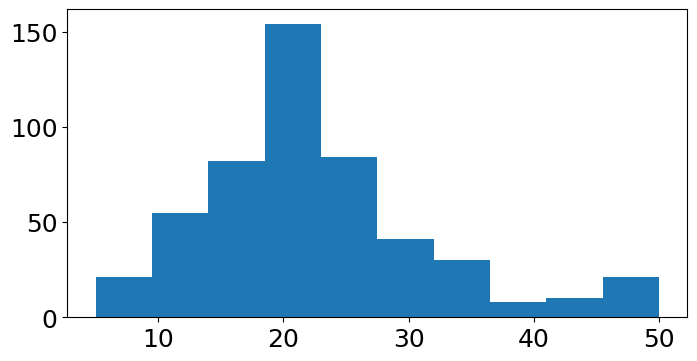
\includegraphics[width=\FigWidth]{figures/practice/chapter-1/sem1-cell36-out0.png}
\caption{Семинар~1: \texttt{medv}. Обратите внимание на правоскошение и отдельные дорогие наблюдения в хвосте.}
\label{fig:p1-shape}
\end{figure}

\begin{figure}[htbp]
\centering
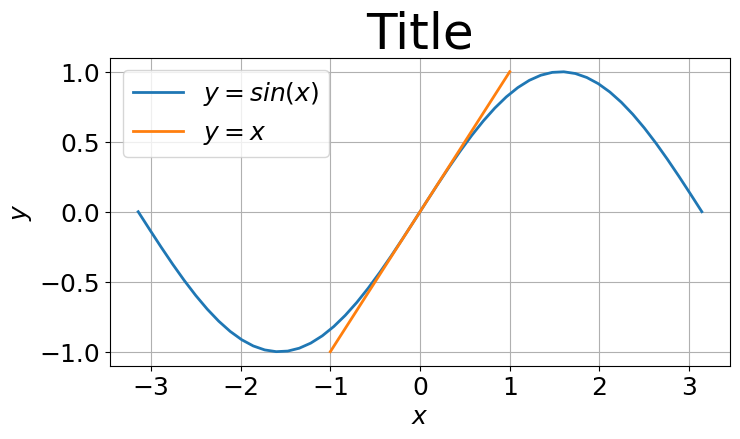
\includegraphics[width=\FigWidth]{figures/practice/chapter-1/sem1-cell09-out0.png}
\caption{Семинар~1: эмпирическая функция распределения \texttt{medv}. На графике видно пологий подъём в левой части и длинный хвост справа.}
\label{fig:p1-ecdf}
\end{figure}

\textbf{Метод и числа.} $\bar x\approx 22{,}5$, медиана $\approx 21{,}2$, $s\approx 9{,}2$.
95\%-й $t$-интервал для $\mathbb E X$: примерно $[20{,}2,\,24{,}8]$; перцентильный бутстреп для $\bar x$ даёт близкий интервал (схема --- рис.~\ref{fig:boot} выше).

\medskip\noindent\textbf{Три вопроса.} \textit{Постановка:} цена жилья в выборке Boston, одна непрерывная переменная.
\textit{Применимость:} сначала форма распределения (гистограмма, ECDF); $t$-ДИ --- при умеренной асимметрии как приближение, медиана и бутстреп --- при сомнении.
\textit{Вывод:} типичная цена около 21--22 тыс.; разброс большой; в отчёте указать асимметрию и не трактовать $t$-ДИ как точный для сильно скошенных данных.\medskip
\paragraph{Связь \texttt{medv} с \texttt{lstat}.}
\textbf{Данные и вопрос.} Предиктор \texttt{lstat} --- доля населения низкого соц.\ статуса; ожидаем отрицательную связь с ценой.

\textbf{График.} Диаграмма рассеяния (рис.~\ref{fig:p1-scatter}) --- почти линейное падение; на pairplot по числовым признакам (рис.~\ref{fig:p1-pair}) видно, что \texttt{lstat} сильнее прочих коррелирует с \texttt{medv}.

\begin{figure}[htbp]
\centering
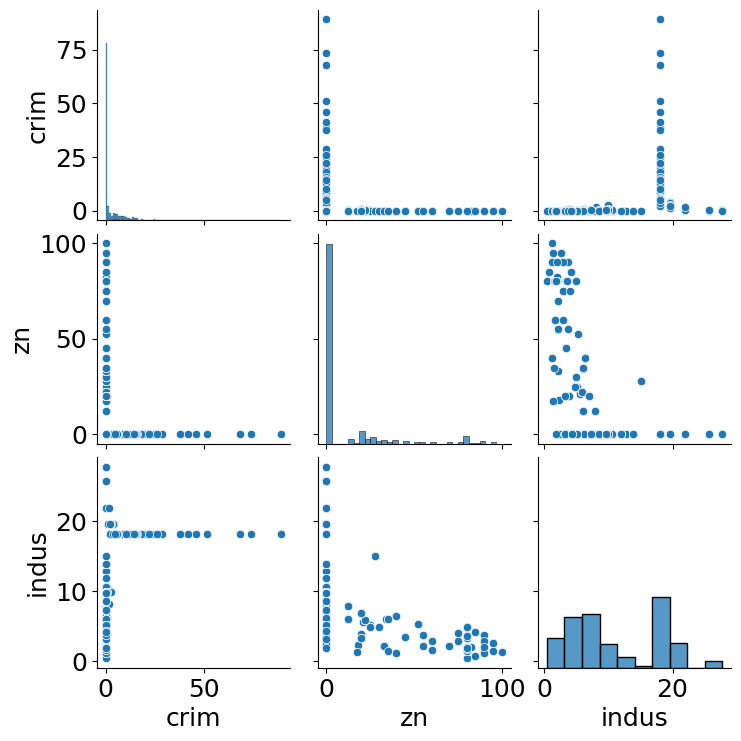
\includegraphics[width=\FigWidth]{figures/practice/chapter-1/sem1-cell45-out0.png}
\caption{Семинар~1: \texttt{medv} и \texttt{lstat}. На графике видно монотонное снижение цены при росте \texttt{lstat}.}
\label{fig:p1-scatter}
\end{figure}
\begin{figure}[htbp]
\centering
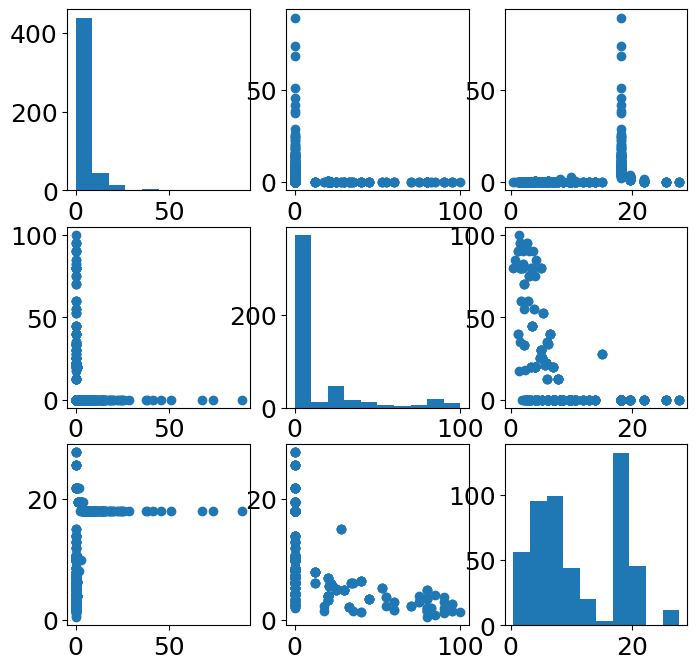
\includegraphics[width=\FigWidth]{figures/practice/chapter-1/sem1-cell47-out0.png}
\caption{Семинар~1: pairplot числовых признаков. Обратите внимание на насыщенный столбец/строку для \texttt{medv}--\texttt{lstat}.}
\label{fig:p1-pair}
\end{figure}

\medskip\noindent\textbf{Три вопроса.} \textit{Постановка:} две непрерывные переменные, исследуем ассоциацию, не причинность.
\textit{Применимость:} scatter и корреляция Пирсона после визуального осмотра; при выбросах --- Спирмен (гл.~\ref{ch:anova}).
\textit{Вывод:} чем выше \texttt{lstat}, тем ниже \texttt{medv}; для отчёта нужна регрессия (гл.~\ref{ch:regression}), здесь --- разведка.\medskip
\paragraph{Домашнее задание sem1.}
Персональная выборка по почте: шаги те же (график $\to$ центр/разброс $\to$ интервал), числа свои; сверяйте форму распределения с рис.~\ref{fig:p1-shape}, а не только с $\bar x$.
\medskip\noindent\textbf{Три вопроса.} \textit{Постановка:} своя непрерывная переменная из задания.
\textit{Применимость:} гистограмма или ECDF, затем центр и ДИ; при асимметрии --- медиана и бутстреп (гл.~\ref{ch:basics}).
\textit{Вывод:} типичный уровень, разброс и оговорка о форме; не цитировать только $\bar x$ без графика.\medskip

По итогам раздела: для каждой задачи --- объекты измерения, график, процедура, 1--3 числа, вывод словами; типичная ошибка --- $t$-интервал при сильной асимметрии без проверки формы.

\section{Контрольные вопросы по теме}

\begin{enumerate}
 \item Чем отличается доверительный интервал от байесовского достоверного интервала, см.~гл.~\ref{ch:bayes}?
 \item Почему выборочная медиана робастнее среднего?
 \item Запишите функцию правдоподобия для $Bin(n,p)$ и ОМП $\hat p$.
 \item Выведите $\hat\mu_{MLE}$ для нормальной выборки через $S(\mu)=0$.
 \item Когда $t$-интервал для среднего предпочтительнее $z$-интервала?
 \item Сравните перцентильный, студентизированный и BCa бутстреп.
 \item Почему бутстреп медианы может быть неточен при $n=15$?
 \item Интерпретируйте p-value в словах, без формулы вероятности $H_0$.
 \item Чем статистическая значимость отличается от практической?
 \item Какие факторы увеличивают мощность критерия?
 \item Что такое статистика в смысле этой главы?
 \item Почему квартет Энскомба важен для практики, если сводные числа уже посчитаны?
 \item Верно ли, что «p-value $=0{,}03$ означает, что $H_0$ верна с вероятностью 3\%»? Объясните.
 \item Чем отличается доверительный интервал от утверждения «$\mu$ лежит в $[a,b]$ с вероятностью 95\%» для одной построенной пары $(a,b)$?
 \item При бутстрепе псевдовыборки берут с возвращением или без? Почему?
 \item Назовите ОМП доли успехов $p$ в модели $Ber(p)$.
 \item Если $n$ очень велико, а размер эффекта мал, может ли p-value быть меньше $\alpha$ при практически неважном эффекте?
 \item Назовите два фактора, от которых растёт мощность критерия при фиксированном $\alpha$.
 \item В каких случаях медиана предпочтительнее $\bar x$ как центральная характеристика?
 \item Связаны ли ЭФР $F_n$ и бутстреп? В чём суть связи?
\end{enumerate}

\chapter{Параметрические и непараметрические критерии}
\label{ch:hypothesis}

В главе~\ref{ch:basics} введена общая схема проверки гипотез: нулевая гипотеза $H_0$, альтернатива $H_1$, статистика $T$ с известным нулевым распределением и p-value как мера экстремальности наблюдения при $H_0$.
Там же показано, что выбор критерия начинается не с формулы, а с постановки вопроса: что именно считается отсутствием эффекта, какие наблюдения независимы, какая шкала у переменной и насколько данные по форме согласуются с предполагаемой моделью.
Настоящая глава развивает этот аппарат в двух направлениях, которые в прикладной работе дополняют друг друга, а не конкурируют.

В \S\ref{sec:parametric} рассматриваются параметрические критерии: предполагается, что выборка порождена распределением из заданного семейства (нормальное, Бернулли), а $H_0$ формулируется через неизвестные параметры.
Если предпосылки разумны, такие процедуры обычно обладают наибольшей мощностью: модель узкая, зато статистика $T$ и её нулевое распределение выводятся точно или асимптотически.
В \S\ref{sec:nonparametric} --- непараметрические методы, которые минимально ограничивают форму распределения и опираются на знаки, ранги или перестановки наблюдений.
Их применяют, когда нормальность сомнительна, хвосты тяжёлые, шкала ординальная или когда $H_0$ касается медианы и всей функции распределения, а не только среднего.

Оба блока опираются на одну идею из гл.~\ref{ch:basics}: при справедливости $H_0$ распределение $T$ известно (точно или асимптотически), что позволяет количественно сопоставить данные с моделью.
Практический маршрут часто выглядит так: сначала визуализация и описательная статистика, затем параметрический критерий при обоснованных предпосылках, и при нарушении предпосылок --- непараметрический аналог или перестановочная проверка.
Примеры с крысами, временем ремонта линий связи и диаметрами шайб в этой главе проиллюстрируют обе ветви этой схемы.

\section{Параметрические критерии}
\label{sec:parametric}

Параметрический критерий применим, когда генеральная совокупность описывается семейством $\{F(\cdot;\theta):\theta\in\Theta\}$ \citep{lehmann2005}; гипотеза касается значения $\theta$ или его подмножества.
Типичные задачи --- сравнение среднего с нормативом, контроль дисперсии, сравнение центров двух групп --- всё это сводится к ограничениям на $\theta$ при фиксированной форме $F$.
Наиболее разработан случай нормальных выборок; для бинарных исходов естественной моделью служит распределение Бернулли.
В обоих случаях p-value вычисляется по той же логике, что и в гл.~\ref{ch:basics}: находим $t_{\text{obs}}=T(x^n)$ и оцениваем, насколько редки такие или более экстремальные значения при $H_0$.

\begin{definition}
Выборка $X^n=(X_1,\ldots,X_n)$ называется нормальной, если $X_i$ независимы и $X_i\sim N(\mu,\sigma^2)$ с неизвестными $\mu$ и $\sigma^2$.
\end{definition}

Для нормальных данных выводятся точные критерии Стьюдента, Фишера и $\chi^2$; при больших $n$ и выполнении условий ЦПТ аналогичные процедуры используют как приближение и для иных распределений.
Общий шаблон повторяется: стандартизируем разность между оценкой параметра и значением под $H_0$, делим на оценку стандартной ошибки и сравниваем полученное $t_{\text{obs}}$ с табличным или вычисленным нулевым распределением.
Различие между конкретными критериями --- в том, какой параметр проверяется и что считается известным ($\sigma$ или только выборка).
Единый маршрут главы можно пройти на одном учебном наборе: сначала Q--Q график и тест Шапиро--Уилка, затем $t$-критерий на среднее, при сомнении~--- Манна--Уитни, при необходимости~--- перестановки.
Если все четыре шага дают согласованный качественный вывод, p-value $t$-критерия интерпретируется увереннее; расхождение (как у времени ремонта линий)~--- сигнал проверить предпосылки, а не подбирать критерий апостериорно.

Z-критерий (известна $\sigma$): это частный случай схемы из гл.~\ref{ch:basics}, когда дисперсия генеральной совокупности задана априори (калиброванный прибор, длительный исторический контроль). Статистика имеет точное стандартное нормальное распределение при $H_0$: \[ H_0\colon \mu=\mu_0,\qquad Z=\frac{\bar X-\mu_0}{\sigma/\sqrt n}\sim N(0,1)\ \text{при}\ H_0.
\] Двусторонний p-value: $2\bigl(1-\Phi(|z_{\text{obs}}|)\bigr)$; односторонние~--- $F_{N(0,1)}(z)$ или $1-F_{N(0,1)}(z)$.
На практике $\sigma$ известна редко; Z-критерий полезен как иллюстрация и в задачах контроля качества с жёстко заданной точностью линии.

Одновыборочный $t$-критерий ($\sigma$ неизвестна): здесь дисперсию оценивают по выборке ($S$), и знаменатель случаен.
Именно поэтому $T$ следует распределению Стьюдента с $n-1$ степенями свободы, а не нормальному: \[ H_0\colon \mu=\mu_0,\qquad T=\frac{\bar X-\mu_0}{S/\sqrt n}\sim St(n-1)\ \text{при}\ H_0.
\] Двусторонний p-value: $2\bigl(1-F_{St(n-1)}(|t_{\text{obs}}|)\bigr)$.
При малых $n$ хвосты $St(\nu)$ тяжелее, чем у $N(0,1)$ (рис.~\ref{fig:z-t-null}), поэтому нельзя подменять $t$-критерий Z-критерием ради упрощения.

Критерий $\chi^2$ на дисперсию: проверяет не центр, а разброс. При нормальности $(n-1)S^2/\sigma^2$ имеет $\chi^2$-распределение: \[ H_0\colon \sigma^2=\sigma_0^2,\qquad \chi^2=\frac{(n-1)S^2}{\sigma_0^2}\sim\chi^2_{n-1}\ \text{при}\ H_0.
\]

Двухвыборочный $t$-критерий (независимые выборки, равные дисперсии): сравнивает средние двух групп при предположении $\sigma_1^2=\sigma_2^2$.
Объединённая оценка дисперсию $S_p^2$ повышает эффективность, но делает критерий уязвимым при её нарушении: \[ H_0\colon \mu_1=\mu_2,\qquad T=\frac{\bar X_1-\bar X_2}{S_p\sqrt{1/n_1+1/n_2}},\quad S_p^2=\frac{(n_1-1)S_1^2+(n_2-1)S_2^2}{n_1+n_2-2}, \] нулевое распределение~--- $St(n_1+n_2-2)$.

Критерий Уэлча (неравные дисперсии): знаменатель $S_1^2/n_1+S_2^2/n_2$, число степеней свободы~--- по Satterthwaite.
Его предпочитают по умолчанию при сравнении групп с разным разбросом (см. примеры с крысами и рабочими часами в этой главе).

Парный $t$-критерий (связанные наблюдения $D_i=X_{1i}-X_{2i}$): сводит пару измерений к одной выборке разностей; типичен для схемы до и после (когнитивные тесты при СДВГ): \[ H_0\colon \mathbb ED=0,\qquad T=\frac{\bar D}{S_D/\sqrt n}\sim St(n-1).
\]

F-критерий (равенство дисперсий): предшествует pooled $t$-критерию: если $\sigma_1^2\neq\sigma_2^2$, объединённая дисперсию вводит систематическую ошибку в тест на средние.
\[ H_0\colon \sigma_1^2=\sigma_2^2,\qquad F=\frac{S_1^2}{S_2^2}\sim F(n_1-1,n_2-1)\ \text{при}\ H_0.
\] Чувствителен к отклонениям от нормальности.
\begin{figure}[htbp]
    \centering
    \begin{subfigure}[b]{\FigWidth}
        \centering
        
\includegraphics[width=\linewidth]{\FigDir/chapter-2/norm.png}
        \caption{$Z$-критерий: $N(0,1)$}
    \end{subfigure}\\[0.6em]
    \begin{subfigure}[b]{\FigWidth}
        \centering
        
\includegraphics[width=\linewidth]{\FigDir/chapter-2/stud.png}
        \caption{$t$-критерий: $St(\nu)$}
    \end{subfigure}
    \caption{Нулевые распределения $Z$- и $t$-критериев; при малых $\nu$ хвосты $t$ тяжелее.}
    \label{fig:z-t-null}
\end{figure}

$t$-критерии чувствительны к выбросам и устойчиво работают при умеренных отклонениях от нормальности, если $n$ достаточно велико (центральная предельная теорема для $\bar X$).
При малых $n$ и заметной асимметрии следует проверять нормальность (график QQ, критерий Шапиро--Уилка) или переходить к непараметрическим аналогам (\S\ref{sec:nonparametric}) --- как мы сделаем для времени ремонта линий связи, где $t$-критерий окажется на грани значимости, а ранговый метод даст более устойчивый вывод.
Критерий Уэлча заменяет объединённую дисперсию $S_p^2$ на $S_1^2/n_1+S_2^2/n_2$ и использует поправку Satterthwaite для числа степеней свободы.
Одностороннюю альтернативу выбирают только если знак эффекта известен до получения данных; иначе p-value можно подогнать под желаемый вывод (пример с упаковкой).

Следующие примеры иллюстрируют одну схему из гл.~\ref{ch:basics}: формулируем $H_0$, вычисляем $T$, сопоставляем с нулевым распределением и интерпретируем $p$ содержательно, не отрывая числа от графика.
Пример: контроль веса упаковки (Z-критерий). На линии расфасовки норма среднего веса~--- 4~г при $\sigma=1$~г (дисперсия стабильна по технологическому регламенту).
Инспекция $n=9$ упаковок дала $\bar x=4{,}6$~г --- заметное, но не очевидное превышение на глаз.
\[ z=\frac{4{,}6-4}{1/\sqrt 9}=1{,}8,\quad p_{\text{двуст.}}\approx 0{,}072,\quad p_{\text{верх.}}\approx 0{,}036.
\] Двусторонняя альтернатива не отвергает $H_0$ при $\alpha=0{,}05$; односторонняя альтернатива о превышении нормы~--- отвергает. Это иллюстрирует опасность выбора альтернативы постфактум: та же выборка и та же $z_{\text{obs}}$, но разные $p$ и разные решения.

Пример: дисперсия объёма инъекции ($\chi^2$). Стандарт требует $\sigma^2=9$~кв.\,мл; при $n=25$ получено $s^2=12$.
Здесь $H_0$ касается разброса, а не среднего --- типичная постановка контроля воспроизводимости дозирования.
\[ \chi^2_{\text{obs}}=\frac{24\cdot 12}{9}\approx 32,\quad p_{\text{двуст.}}\approx 0{,}25 \] --- отклонения от стандарта статистически незначимы, хотя точечная оценка превышает норму. Содержательный вывод: наблюдаемое превышение может быть случайной флуктуацией при текущем объёме выборки.

Пример: программа ведения беременности ($t$-критерий). Для женщин за чертой бедности базовое среднее веса новорождённых~--- 2800~г. После программы при $n=25$: $\bar x=3075$~г, $s=500$~г. Одновыборочный $t$-критерий --- прямое применение схемы сравнения среднего с нормативом при неизвестной $\sigma$.
\[ t=\frac{3075-2800}{500/\sqrt{25}}=2{,}75,\quad p_{\text{двуст.}}\approx 0{,}011.
\] Программа статистически значимо связана с увеличением веса; размер эффекта $\approx 275$~г следует оценивать содержательно.
Содержательный вопрос здесь шире p-value: клинически значим ли прирост 275~г для новорождённого в данной популяции? Статистика указывает на отличие от нулевого флуктуационного шума; врач и эпидемиолог решают, достаточен ли он для рекомендации программы.
Такой разделённый вывод~--- норма прикладного анализа, а не противоречие статистике.

Пример: измерения скорости света. В классическом эксперименте Michelson зафиксировано $n=100$ измерений скорости света методом вращающегося зеркала --- редкий случай большой выборки при лабораторной точности.
Выборочное среднее $\bar x\approx 2{,}9985\times 10^5$~м/с, стандартное отклонение $s\approx 79$~м/с. На рис.~\ref{fig:speed-ttest} показано распределение наблюдений и 95\%-й доверительный интервал для $\mu$ (см. гл.~\ref{ch:basics}).

\begin{figure}[htbp]
    \centering
    
\includegraphics[width=\FigWidth]{\FigDir/chapter-2/qqplot.png}
    \caption{Распределение измерений скорости света и интервал для среднего.}
    \label{fig:speed-ttest}
\end{figure}

Проверка $H_0\colon \mu=3{,}0000\times 10^5$ против двусторонней альтернативы даёт $t\approx -18{,}7$ и $p\approx 3\times 10^{-34}$: систематическое отклонение среднего от теоретического значения статистически значимо.
Содержательно это не опровержение физики, а сигнал о погрешности прибора или модели измерения; график подтверждает близость данных к нормальному распределению, что оправдывает $t$-критерий.
Важно: отклонение $H_0\colon\mu=\mu_0$ не означает отказ от нормальности --- отвергается конкретное значение среднего, а не форма $F$.

Пример: продолжительность жизни крыс. Зафиксирована продолжительность жизни крыс при двух режимах питания: restricted ($n_1=106$) и ad libitum ($n_2=89$).
Средние составляют $\bar x_1\approx 969$ и $\bar x_2\approx 684$~дней --- крупный содержательный сдвиг; вопрос в том, насколько он устойчив к предпосылкам $t$-критерия.

Двухвыборочный критерий Уэлча даёт $p\approx 3\times 10^{-16}$: ограничение калорийности ассоциировано с более длительной жизнью.
Ящики с усами на рис.~\ref{fig:mannwhitney} иллюстрируют сдвиг распределений; тот же вывод подтверждается ранговым критерием Манна--Уитни ($p\approx 8\times 10^{-17}$, см. \S\ref{sec:nonparametric}).
Этот пример связывает обе части главы: параметрический тест даёт убедительный результат, а непараметрический --- независимую проверку без предположения о нормальности сроков жизни.

Пример: рабочие часы (GSS, критерий Уэлча). Сравнение числа рабочих часов в неделю у работающих неполный день в 1974 ($n_1=108$) и 2014 ($n_2=196$) годах: среднее увеличилось примерно на 2{,}57~часа, $p\approx 0{,}027$ (критерий Уэлча).
Распределения асимметричны и с тяжёлыми хвостами; ящик с усами (рис.~\ref{fig:hpw}) полезен для интерпретации: медианы и квартили показывают сдвиг иначе, чем одно $\bar x$.

\begin{figure}[htbp]
    \centering
    
\includegraphics[width=\FigWidth]{\FigDir/chapter-2/hpw.png}
    \caption{Рабочие часы в неделю: сравнение двух лет.}
    \label{fig:hpw}
\end{figure}

Пример: когнитивные тесты при СДВГ. В исследовании СДВГ содержатся результаты теста внимания ($D0$~--- до лечения, $D60$~--- через 60~дней) для $n=24$ детей.
Среднее изменение $\bar d\approx 4{,}96$ балла, медиана~--- $5$.
Парная структура данных обязательна: каждое измерение после сопоставлено с до у того же ребёнка у того же ребёнка.

Парный $t$-критерий для $H_0\colon \mathbb ED=0$ даёт $p\approx 0{,}004$: метилфенидат статистически значимо улучшает показатель.
Парный критерий знаковых рангов Уилкоксона даёт $p\approx 0{,}004$ --- вывод устойчив к отказу от нормальности разностей; мы вернёмся к парным ранговым процедурам в \S\ref{sec:nonparametric}.

Пример: сравнение дисперсий (F-критерий). При сравнении прочности керамики из двух партий по 220 изделий критерий Фишера на $H_0\colon\sigma_1^2=\sigma_2^2$ может дать $p\approx 0{,}17$ при визуально близких дисперсиях.
F-критерий особенно чувствителен к отклонениям от нормальности, поэтому незначимый результат F-критерия не лицензирует pooled $t$ без графика.
Перед применением pooled $t$-критерия имеет смысл проверить равенство дисперсий; при отклонении $H_0$~--- критерий Уэлча.

\begin{figure}[htbp]
    \centering
    
\includegraphics[width=\FigWidth]{\FigDir/chapter-2/fish.png}
    \caption{Нулевое распределение F-критерия.}
    \label{fig:f-test}
\end{figure}

\label{sec:gof}
Многие параметрические процедуры предполагают нормальность.
Проверка $H_0\colon X\sim N(\mu,\sigma^2)$ --- частный случай критерия согласия (goodness-of-fit): $H_0$ задаёт полное распределение (возможно, с оцениваемыми параметрами).
Логика та же, что в гл.~\ref{ch:basics}: при $H_0$ статистика согласия имеет известное распределение; большие значения означают плохое совпадение данных с моделью.
На практике Q--Q график часто информативнее формального $p$: он показывает где именно модель расходится с выборкой (центр, хвосты, асимметрия).

Критерий Харке--Бера: ориентирован на асимметрию и тяжесть хвостов через моменты третьего и четвёртого порядка: \[ JB=\frac{n}{6}\left(\hat\gamma_1^2+\frac{\hat\gamma_2^2}{4}\right) \sim\chi^2_2\ \text{при}\ H_0, \] где $\hat\gamma_1$, $\hat\gamma_2$~--- выборочные асимметрия и эксцесс. Чувствителен к выбросам: один экстремальный $x_i$ может раздуть $\hat\gamma_2$.

Критерий согласия Пирсона ($\chi^2$ по ячейкам): классический подход для сгруппированных данных; разбиение области значений на $K$ интервалов, $n_i$~--- частоты, $p_i$~--- теоретические вероятности при $H_0$: \[ \chi^2=\sum_{i=1}^K\frac{(n_i-np_i)^2}{np_i}\sim\chi^2_{K-1-r}, \] $r$~--- число оценённых параметров. Требует $np_i\gtrsim 5$ в большинстве ячеек; иначе асимптотика $\chi^2$ ненадёжна.

Колмогорова--Смирнова (одновыборочный; Лиллиефорс~--- при подстановке $\hat\mu$, $\hat\sigma$): сравнивает эмпирическую и теоретическую функции распределения по максимальному вертикальному зазору: \[ D=\sup_x|F_n(x)-F_0(x)|; \] табличное нулевое распределение. Слабее чувствителен к хвостам, чем JB или Q--Q-диагностика на рис.~\ref{fig:qq-norm}.

Шапиро--Уилка: статистика $W$ на основе порядковых статистик и табличных коэффициентов; рекомендуется для формальной проверки нормальности при умеренных $n$, когда нужен одно числовое p-value дополнительно к графику.
\begin{figure}[htbp]
 \centering
 \begin{subfigure}[b]{\FigWidth}
 \centering
 
\includegraphics[width=\linewidth]{\FigDir/chapter-2/qqplot.png}
 \caption{Нормальная выборка}
 \end{subfigure}\\[0.6em]
 \begin{subfigure}[b]{\FigWidth}
 \centering
 
\includegraphics[width=\linewidth]{\FigDir/chapter-2/qq_tails.png}
 \caption{Отклонения на хвостах}
 \end{subfigure}
 \caption{Q--Q графики: согласие с нормалью и типичные отклонения на хвостах.}
 \label{fig:qq-norm}
\end{figure}

\begin{figure}[htbp]
 \centering
 
\includegraphics[width=\FigWidth]{\FigDir/chapter-2/qq_skewness.png}
 \caption{Q--Q график при асимметрии выборки.}
 \label{fig:qq-skew}
\end{figure}

Рекомендуемый порядок действий:
\begin{enumerate}
 \item если данные явно дискретны или бинарны~--- специализированный метод;
 \item построить Q--Q plot; при умеренных отклонениях можно применять
устойчивые процедуры ($t$-критерий);
 \item для критериев, чувствительных к форме (F на дисперсии), при сомнениях~---
Шапиро--Уилк;
 \item на очень малых $n$ формальные критерии малоинформативны;
 на очень больших~--- отвергают даже ничтожные отклонения от нормальности.
\end{enumerate}
Незначимый тест на нормальность не доказывает идеальную нормальность --- лишь отсутствие статистически различимых отклонений при данном $n$.
При сомнениях разумно дублировать вывод непараметрическим критерием (\S\ref{sec:nonparametric}), как в примере с временем ремонта.
Важно различать два типа расхождения с нормальностью: формальный тест может не отвергнуть $H_0$ при малом $n$, хотя график уже показывает асимметрию; при большом $n$~--- наоборот, отвергает при ничтожном отклонении. Поэтому критерии согласия~--- не пропуск к $t$-тесту, а элемент сочетания графика и формального теста: сначала глаз, затем статистика, затем робастная проверка при содержательных сомнениях.

Пусть $\ell(\theta)=\log L(X^n;\theta)$~--- логарифм функции правдоподобия, $\hat\theta$~--- ОМП при отсутствии ограничений, $\theta_0$~--- значение под $H_0\colon \theta=\theta_0$.
Идея LR повторяет логику гл.~\ref{ch:basics}: сравниваем, насколько сильно ограниченная модель ($H_0$) проигрывает полной в подгонке к данным.
\begin{definition}
Статистика отношения правдоподобия (LR) равна
\[
\Lambda(X^n)=-2\log\frac{L(X^n;\theta_0)}{L(X^n;\hat\theta)} =-2\bigl(\ell(\theta_0)-\ell(\hat\theta)\bigr).
\]
\end{definition}
При стандартных регулярных условиях и справедливости $H_0$ асимптотически $\Lambda\sim\chi^2_r$, где $r$~--- число независимых ограничений в $H_0$.
LR-критерий универсален: для нормальной выборки проверка $\mu=\mu_0$ при известной $\sigma$ эквивалентна $Z$-критерию; при неизвестной $\sigma$~--- $t$-критерию.
Пример LR: для $H_0\colon\mu=\mu_0$ в нормальной модели $\Lambda$ монотонно связана с $t^2$; большое $\Lambda$ означает, что ограниченная модель с $\mu=\mu_0$ существенно хуже подгоняет данные, чем полная. Эта логика переносится на регрессию (гл.~\ref{ch:regression}), где LR-тест сравнивает вложенные GLM.
Преимущество LR~--- единая схема для сложных вложенных моделей (регрессия, GLM; см. гл.~\ref{ch:regression}).
На уровне этой главы LR связывает разрозненные $t$- и $\chi^2$-формулы в один принцип: чем больше $\Lambda$, тем менее правдоподобна $H_0$.

Для $X_i\sim Ber(p)$ i.i.d. типична проверка доли успехов: \[ H_0\colon p=p_0,\qquad \hat p=\bar X,\qquad \Lambda=-2\log\frac{L(p_0)}{L(\hat p)}\ \dot\sim\ \chi^2_1\ \text{при}\ H_0.
\] Точный биномиальный критерий: при $S=\sum X_i$ под $H_0$ $S\sim Bin(n,p_0)$; двусторонний p-value~--- сумма вероятностей реализаций не более вероятных, чем наблюдаемая.
Биномиальный критерий предпочтителен при малых $n$ и экстремальных $p_0$; LR и асимптотика нормального приближения $\hat p$ согласуются при $np_0(1-p_0)\gtrsim 5$.
Бинарная модель напоминает эксперимент с мышами и зеркалом (\S\ref{sec:nonparametric}): там $H_0$ сформулирована через медиану доли времени, а здесь --- через параметр $p$ при явной модели Бернулли.

\begin{itemize}
 \item Применять двухвыборочный $t$-критерий с объединённой дисперсией
 при явно различных $S_1^2$ и $S_2^2$ без проверки или перехода к критерию Уэлча.
 \item Интерпретировать значимый одновыборочный $t$-критерий как
 доказательство ненормальности~--- отклоняется конкретное значение $\mu_0$, а не форма распределения.
 \item Заменять биномиальный критерий нормальным при $n<20$
 и $p$ близком к $0$ или $1$.
 \item Считать незначимый тест на нормальность доказательством
 идеальной нормальности данных.
\end{itemize}

\section{Непараметрические критерии}
\label{sec:nonparametric}

Непараметрические критерии не предполагают конкретного семейства распределений; $H_0$ формулируется через медианы, функции распределения или симметрию.
Цена универсальности~--- меньшая мощность при выполнении параметрических предпосылок: если данные действительно нормальны, $t$-критерий использует информацию о величине отклонений, а знаковый критерий --- только их направление.
Зато при асимметрии, выбросах и ординальных шкалах непараметрические процедуры часто дают единственный честный p-value.
Примеры с крысами, временем ремонта и шайбами показывают, когда параметрический и непараметрический ответ совпадают, а когда расходятся.

\begin{definition}
Критерий знаков использует число наблюдений по одну сторону от порога (или число положительных разностей) при $H_0$ о медиане; при непрерывности нулевое распределение биномиальное.
\end{definition}

Одновыборочный критерий знаков ($H_0\colon \med X = m_0$): статистика $S^+=\#\{i\colon X_i>m_0\}$; при $H_0$ и непрерывном $F_X$ $S^+\sim Bin(n,1/2)$.
Интуиция: при верной $H_0$ о пороге $m_0$ наблюдения по разные стороны порога должны встречаться примерно поровну.

Парный критерий знаков ($H_0\colon \med D=0$ для $D_i=X_i-Y_i$): $S^+=\#\{i\colon D_i>0\}\sim Bin(n,1/2)$ при симметрии $D$ относительно нуля.
Критерий знаков применим при цензурированных данных (известен только знак отклонения от порога), ординальных шкалах и тяжёлых хвостах, где ранговые методы нестабильны.
Используется лишь информация о знаке, поэтому мощность меньше, чем у ранговых критериев, но предпосылки слабее.

Пример: предпочтение зеркала у мышей. В эксперименте с зеркалом у мышей приведены доли времени ($n=16$), проведённые мышью в камере с зеркалом --- непрерывные доли на $(0,1)$, но без явной нормальной модели.
Средняя доля $\bar x\approx 0{,}475$; проверка $H_0\colon \med X=0{,}5$ критерием знаков (число наблюдений $>0{,}5$ равно $6$) даёт $p\approx 0{,}79$: данных против симметрии вокруг $0{,}5$ недостаточно.
При этом $\bar x<0{,}5$, что иллюстрирует различие среднего и медианы (см. гл.~\ref{ch:basics}): критерий знаков отвечает на вопрос о медиане, а не о среднем арифметическом.
Этот пример --- мост от бернуллиевской логики доли успехов к непараметрической формулировке без жёсткой модели $Ber(p)$.

Критерий Уилкоксона (одна выборка, $H_0\colon \med X=m_0$): ранги $R_i=\operatorname{rank}|X_i-m_0|$, статистика $W^+=\sum_{i\colon X_i>m_0} R_i$; нулевое распределение~--- табличное или точное перебором $2^n$ знаков.

Парный Уилкоксон для связанных выборок~--- то же для $D_i$.

Критерий Манна--Уитни (две независимые выборки, $H_0\colon F_1=F_2$): $U_1=\#\{(i,j)\colon X_{1i}>X_{2j}\}$; при $H_0$ распределение $U_1$ таблично; для больших $n_1,n_2$ применяют нормальное приближение.
Важно помнить: $H_0$ здесь шире равенства средних --- это полное совпадение распределений; значимый результат может отражать и разную форму.
\begin{figure}[htbp]
 \centering
 
\includegraphics[width=\FigWidth]{\FigDir/chapter-2/signrank.png}
 \caption{Нулевое распределение критерия знаковых рангов (иллюстрация).}
 \label{fig:signrank}
\end{figure}

Ранговые критерии требуют непрерывности (или мало совпадений) и для парного Уилкоксона~--- примерной симметрии распределения разностей при $H_0$.
Отклонение $H_0$ может отражать асимметрию, а не только сдвиг медианы; диагностика формы обязательна.
На рис.~\ref{fig:mannwhitney} сопоставлены распределения продолжительности жизни крыс (см. параметрический пример с крысами); ранговый критерий не предполагает нормальности и подтверждает различие групп тем же качественным выводом, что и критерий Уэлча, но другим путём вычисления $p$.

\begin{figure}[htbp]
 \centering
 
\includegraphics[width=\FigWidth]{\FigDir/chapter-2/mann.png}
 \caption{Сравнение групп питания крыс: гистограммы и ящики с усами.}
 \label{fig:mannwhitney}
\end{figure}

Пример: время ремонта линий связи. Зафиксировано время устранения неисправности (в часах) для операторов ILEC ($n_1=1664$) и CLEC ($n_2=23$) --- типичная прикладная задача с сильной асимметрией и множеством нулей (мгновенное устранение).
Средние: $\bar x_{\text{ILEC}}\approx 8{,}4$, $\bar x_{\text{CLEC}}\approx 16{,}5$.
Критерий Уэлча даёт $p\approx 0{,}06$ (на границе $\alpha=0{,}05$), тогда как Манна--Уитни~--- $p\approx 0{,}001$.

Распределение времени ремонта сильно асимметрично (много нулей и длинный правый хвост), что нарушает предпосылки $t$-критерия; ранговый критерий устойчивее к выбросам и указывает на систематически более длительное устранение неисправностей у CLEC.
Здесь непараметрический вывод не противоречит параметрическому --- он уточняет его: при сомнительной нормальности и асимметрии опираться на $t$ при $\alpha=0{,}05$ рискованно, тогда как ранги дают устойчивый сигнал.
Ящик с усами (рис.~\ref{fig:boxplot}) показывает сдвиг медианы и хвостов нагляднее, чем одна пара $\bar x$.

\begin{figure}[htbp]
 \centering
 
\includegraphics[width=\FigWidth]{\FigDir/chapter-2/boxplot.png}
 \caption{Ящик с усами: медиана, квартили и выбросы.}
 \label{fig:boxplot}
\end{figure}

Для проверки $H_0\colon F_1=F_2$ (полное совпадение распределений, не только средних) используют статистики, основанные на ЭФР.
Это ближе к духу гл.~\ref{ch:basics}: $H_0$ задаёт полную модель (здесь --- идентичность двух $F$), а $T$ измеряет расхождение данных с ней.

Критерий Смирнова (двухвыборочный Колмогоров--Смирнов): \[ D=\sup_x|F_{n_1}(x)-F_{n_2}(x)|; \] нулевое распределение табличное при $H_0$.

Критерий Андерсона (модификация Крамера--фон Мизеса для двух выборок): статистика на основе рангов объединённой выборки; чувствительнее к различиям в хвостах, чем Смирнов.
Отличие от Манна--Уитни: $H_0$ шире (равенство всей $F$), а не только сдвиг; при разных формах, но равных медианах, критерии согласия и ранговые критерии могут вести себя по-разному.
Для крыс и времени ремонта Манна--Уитни и $t$-критерий отвечали на вопрос о сдвиге; KS/Андерсон дополнили бы картину, если бы подозревали различие форм при близких медианах.

\begin{definition}
Перестановочный критерий строит нулевое распределение статистики $T$, перебирая перестановки или разбиения, равновероятные при $H_0$; p-value --- доля перестановок с не менее экстремальным $T$, чем наблюдаемое.
\end{definition}

Это тот же каркас, что в гл.~\ref{ch:basics}, но вместо табличного $F_T$ распределение $T$ симулируют из данных при верной $H_0$:
\begin{itemize}
 \item Одна выборка, $H_0\colon\mathbb EX=m_0$, симметрия $F$:
 $T=\sum(X_i-m_0)$; нулевое распределение~--- $2^n$ знаков.
 \item Связанные выборки: $D_i=X_{1i}-X_{2i}$, перебор знаков $D_i$.
 \item Независимые выборки, $H_0\colon F_1=F_2$:
 объединить выборки и всеми $\binom{n_1+n_2}{n_1}$ способами разбить на группы; $T=\bar X_1-\bar X_2$ (или функция рангов).
\end{itemize}
p-value~--- доля перестановок с $|T|\geq|t_{\text{obs}}|$ (или односторонне).
Выбор между перестановками, бутстрепом и табличным $t$-критерием зависит от того, что именно является $H_0$: равенство $F_1=F_2$, равенство медиан или только равенство средних при нормальности.
Перестановки наиболее строги по предпосылкам; бутстреп гибче, но не центрирует нулевое распределение при нарушении $F_1=F_2$.
На практике начинают с обоснованной параметрической процедуры и добавляют непараметрическую проверку, как в примерах с крысами и ADHD.
При большом $n_1+n_2$~--- случайная подвыборка из $10^4$--$10^5$ перестановок; СКО оценки $p$ порядка $\sqrt{p(1-p)/|G'|}$.
Перестановочный критерий при $H_0\colon F_1=F_2$ проверяет полное равенство распределений (сдвиг как частный случай), тогда как бутстреп для разности средних (гл.~\ref{ch:basics}) не требует равенства $F$, но даёт приближённый p-value. Перестановки~--- без возвращения; бутстреп~--- с возвращением; нулевое распределение перестановочного $T$ центрировано в значении при $H_0$, бутстреп-распределение~--- в $\hat\theta$.
Если предпосылки перестановочного критерия выполнены, он точнее и обычно мощнее бутстреп-аналога; бутстреп гибче при нарушении $F_1=F_2$.
\begin{figure}[htbp]
 \centering
 
\includegraphics[width=\FigWidth]{\FigDir/chapter-2/ranksum10.png}
 \caption{Нулевое распределение ранговой статистики (иллюстрация).}
 \label{fig:ranksum}
\end{figure}

Пример: диаметры шайб (перестановки и ранги). При проверке соответствия среднего диаметра шайб нормативу ($H_0\colon \mathbb EX=m_0$ при симметрии) критерий знаковых рангов может дать $p\approx 0{,}067$, перестановочный критерий с $T=\sum(X_i-m_0)$~--- $p\approx 0{,}10$: оба не отвергают $H_0$ при $\alpha=0{,}05$, но используют разную информацию (ранги против суммы отклонений).
Это напоминает пример с мышами: при близком к границе $p$ выбор статистики и предпосылок меняет решение сильнее, чем кажется из одной цифры.
Для шайб параметрический $t$-критерий был бы уместен при нормальности; перестановки и ранги дают проверку без жёсткой формы $F$.

\begin{itemize}
 \item Считать непараметрический критерий полностью свободным от предпосылок: симметрия, независимость и связь $H_0$ с медианой или $F$ остаются обязательными.
 \item Выбирать Манна--Уитни как проверку разности средних:
 $H_0$ формулируется как равенство функций распределения; при разных формах, но равных медианах критерий может давать значимый результат.
 \item Игнорировать связность пар в задаче ADHD: двухвыборочный
 критерий вместо парного завышает ошибку I рода.
 \item Путать двухвыборочный KS (равенство $F$) с критерием на сдвиг средних.
\end{itemize}
При написании отчёта по сравнению двух групп полезна явная таблица: цепочку предпосылки, параметрический тест, робастный тест и вывод. Для крыс обе колонки совпадают; для ремонта линий~--- нет; для шайб все три процедуры близки к границе $\alpha$. Такая таблица снимает соблазн цитировать только удобное p-value.

Сопоставление критериев на одной задаче. Рассмотрим сравнение времени сборки детали (с) на двух линиях ($n_1=n_2=35$).
Ящики с усами показывают сдвиг медиан и несколько выбросов на линии~B.
Q--Q графики по группам: линия~A близка к нормали, линия~B~--- с лёгкой асимметрией. Левена даёт $p=0{,}12$; F на дисперсии~--- $p=0{,}18$: объединённый $t$ допустим, но критерий Уэлча~--- безопаснее по умолчанию.

Численно: $\bar x_A=12{,}4$, $\bar x_B=14{,}1$, Уэлч $p=0{,}04$, Манна--Уитни $p=0{,}02$, разность медиан $\approx 1{,}5$~с. Перестановочный тест с $T=\bar x_A-\bar x_B$ даёт $p=0{,}05$. Картина согласованная: линия~B медленнее; ранги чуть увереннее параметрического теста на границе $\alpha=0{,}05$.

В отчёте фиксируем цепочку: (1)~независимость наблюдений (разные детали); (2)~диагностика формы; (3)~$H_0\colon\mu_A=\mu_B$; (4)~$T$ и $p$; (5)~размер эффекта 1{,}7~с и его стоимость в производстве.
Если бы Q--Q показал сильную ненормальность, в тексте доминировали бы Манна--Уитни и перестановки, а $t$-критерий~--- как чувствительность, не как единственный аргумент. Этот шаблон связывает параметрический и непараметрический блоки главы в одну историю.

\section{Асимптотические критерии и критерии согласия для распределений}
\label{sec:theory-ch2}

Асимптотические критерии Вальда и меток (score). Для регулярного параметрического семейства $F(x,\theta)$, $\ell(\theta)=\log L(X^n;\theta)$, $\hat\theta_{\mathrm{MLE}}=\argmax_\theta\ell(\theta)$, $S(\theta)=\partial\ell/\partial\theta$, $I(\theta)=-\partial^2\ell/\partial\theta^2$.

\begin{critcard}{Критерий Вальда}
выборка: &
$X^n=(X_1,\ldots,X_n)$, $X\sim F(x,\theta)$ \\
нулевая гипотеза: &
$H_0\colon\theta=\theta_0$ \\
альтернатива: &
$H_1\colon\theta<\neq>\theta_0$ \\
статистика: &
$Z_W(X^n)=\dfrac{\hat\theta_{\mathrm{MLE}}-\theta_0}{\sqrt{\mathbb{D}\hat\theta_{\mathrm{MLE}}}}$
(на практике $\mathbb{D}\hat\theta_{\mathrm{MLE}}\approx I^{-1}(\hat\theta_{\mathrm{MLE}})$) \\
нулевое распределение: &
$Z_W\sim N(0,1)$ при $H_0$ \\
\end{critcard}
Достигаемый уровень значимости (piecewise): \[ p(Z_W)=\begin{cases} 1-F_{N(0,1)}(Z_W), & H_1\colon\theta>\theta_0,\\[4pt] F_{N(0,1)}(Z_W), & H_1\colon\theta<\theta_0,\\[4pt] 2\bigl(1-F_{N(0,1)}(|Z_W|)\bigr), & H_1\colon\theta\neq\theta_0.
\end{cases}
\] Критерий Вальда использует информацию о правдоподобии только в $\hat\theta_{\mathrm{MLE}}$; на конечных $n$ часто хуже LR и score.

\begin{critcard}{Критерий меток (score, Лагранжа)}
выборка: &
$X^n=(X_1,\ldots,X_n)$, $X\sim F(x,\theta)$ \\
нулевая гипотеза: &
$H_0\colon\theta=\theta_0$ \\
альтернатива: &
$H_1\colon\theta<\neq>\theta_0$ \\
статистика: &
$Z_S(X^n)=\dfrac{S(\theta_0)}{\sqrt{I(\theta_0)}}$ \\
нулевое распределение: &
$Z_S\sim N(0,1)$ при $H_0$ \\
\end{critcard}
\[ p(Z_S)=\begin{cases} 1-F_{N(0,1)}(Z_S), & H_1\colon\theta>\theta_0,\\[4pt] F_{N(0,1)}(Z_S), & H_1\colon\theta<\theta_0,\\[4pt] 2\bigl(1-F_{N(0,1)}(|Z_S|)\bigr), & H_1\colon\theta\neq\theta_0.
\end{cases}
\] Для $X_i\sim\mathrm{Ber}(p)$: $Z_S=\dfrac{\hat p-p_0}{\sqrt{p_0(1-p_0)/n}}$, $Z_W=\dfrac{\hat p-p_0}{\sqrt{\hat p(1-\hat p)/n}}$ (асимптотически эквивалентны LR).

$Z$-критерии для двух долей. Независимые выборки $X_1^{n_1}$, $X_2^{n_2}$~--- независимые, $X_k\sim\mathrm{Ber}(p_k)$.
В таблице $2\times 2$: в первой выборке $a$ единиц из $n_1$, во второй $b$ из $n_2$; $\hat p_1=a/n_1$, $\hat p_2=b/n_2$, объединённая оценка $P=(\hat p_1 n_1+\hat p_2 n_2)/(n_1+n_2)$.

\begin{critcard}{$Z$-критерий: разность двух долей (независимые)}
выборки: &
$X_1^{n_1}$, $X_2^{n_2}$ независимы, $X_k\sim\mathrm{Ber}(p_k)$ \\
нулевая гипотеза: &
$H_0\colon p_1=p_2$ \\
альтернатива: &
$H_1\colon p_1<\neq>p_2$ \\
статистика: &
$Z=\dfrac{\hat p_1-\hat p_2}{\sqrt{P(1-P)\bigl(\frac1{n_1}+\frac1{n_2}\bigr)}}$ \\
нулевое распределение: &
$N(0,1)$ \\
\end{critcard}
p-value~--- по той же кусочно-заданной схеме, что для $Z_W$.
Пример: $n_1=100$, $t_1=3$ дефекта; $n_2=200$, $t_2=5$~--- $H_0$ о равенстве долей дефектных не отвергается ($p\approx 0{,}8$).

Связанные выборки. Одни и те же $n$ объектов, два бинарных признака; таблица $2\times 2$: $e,h$~--- совпадения, $f,g$~--- несовпадения ($f$~--- несовпадения знаков признаков).

\begin{critcard}{$Z$-критерий: разность двух долей (связанные)}
выборки: &
$X_1^n$, $X_2^n$ связаны, $X_k\sim\mathrm{Ber}(p_k)$ \\
нулевая гипотеза: &
$H_0\colon p_1=p_2$ \\
альтернатива: &
$H_1\colon p_1<\neq>p_2$ \\
статистика: &
$Z=\dfrac{f-g}{\sqrt{f+g-(f-g)^2/n}}
=\dfrac{\hat p_1-\hat p_2}{\sqrt{\dfrac{f+g}{n^2}-\dfrac{(f-g)^2}{n^3}}}$ \\
нулевое распределение: &
$N(0,1)$ \\
\end{critcard}
Используют только дискордантные пары $(f,g)$, совпадения $e,h$ не входят в $Z$.
Пример (одобрение премьер-министра, $n=1600$): $e=794$, $f=150$, $g=86$, $h=570$; $H_0$ о неизменности рейтинга~--- $p\approx 2{,}8\times 10^{-5}$ (связанная схема), против $p\approx 0{,}022$ при ошибочном анализе как двух независимых выборок.

Критерий Ансари--Брэдли. Сравнение дисперсий при равных медианах (или после центрирования).
Объединённый вариационный ряд $X_{(1)}\le\cdots\le X_{(N)}$, $N=n_1+n_2$; ранги $\widetilde{\rank}$ присваивают от краёв к центру: $1,2,3,\ldots,3,2,1$.
$R_1=\sum_{i=1}^{n_1}\widetilde{\rank}(X_{1i})$~--- сумма таких рангов в первой группе.

\begin{critcard}{Критерий Ансари--Брэдли}
выборки: &
$X_1^{n_1}$, $X_2^{n_2}$ независимы; $\med X_1=\med X_2$ \\
нулевая гипотеза: &
$H_0\colon \mathbb{D}X_1=\mathbb{D}X_2$ \\
альтернатива: &
$H_1\colon \mathbb{D}X_1<\neq>\mathbb{D}X_2$ \\
статистика: &
$R_1(X_1^{n_1},X_2^{n_2})=\sum_{i=1}^{n_1}\widetilde{\rank}(X_{1i})$ \\
нулевое распределение: &
табличное при $H_0$ \\
\end{critcard}
Пример: вес свинцовых слитков у двух поставщиков, средние в норме; $H_0$ о равенстве дисперсий отвергается ($p\approx 0{,}014$).
 Перед применением проверьте предпосылку о центрах; иначе значимый результат может отражать сдвиг, а не разброс.

Критерии согласия по ЭФР (одна выборка). Семейство статистик строится на различии $F_n(x)$ и $F_0(x)$ (при оцениваемых параметрах нулевое распределение корректируют, как у Лиллиефорса для нормали).

Крамера--фон Мизеса (интеграл Смирнова).\[ W^2=\int_{-\infty}^{\infty}\bigl(F_n(x)-F(x)\bigr)^2\,dF(x).
 \]

Андерсона--Дарлинга.\[ A^2=\int_{-\infty}^{\infty} \frac{\bigl(F_n(x)-F(x)\bigr)^2}{F(x)\bigl(1-F(x)\bigr)}\,dF(x).
\] Вес $[F(1-F)]^{-1}$ усиливает вклад хвостов: при подозрении на тяжёлые хвосты AD предпочтительнее Колмогорова--Смирнова, чувствительного прежде к центру распределения.

\begin{critcard}{Критерий Андерсона--Дарлинга (одна выборка)}
выборка: &
$X^n=(X_1,\ldots,X_n)$ \\
нулевая гипотеза: &
$H_0\colon X\sim F_0$ (параметры $F_0$ фиксированы или оценены по выборке) \\
альтернатива: &
$H_1\colon H_0$ неверна \\
статистика: &
$A^2$ (интеграл выше; в ПО~--- по $F_n$ и $F_0$) \\
нулевое распределение: &
табличное / с поправкой при подстановке $\hat\mu$, $\hat\sigma$ \\
\end{critcard}
На практике AD дополняют Q--Q график: формальный $p$ при большом $n$ может отвергнуть ничтожные отклонения, при малом $n$~--- не заметить асимметрию, видную на графике.

Связь с другими критериями. Колмогоров: $D=\sup_x|F_n(x)-F(x)|$; критерий Пирсона~--- по ячейкам гистограммы ($\chi^2$). AD и $W^2$~--- промежуточный класс по чувствительности к форме; двухвыборочный критерий Андерсона (модификация $W^2$ по рангам объединённой выборки) проверяет $H_0\colon F_1=F_2$ целиком, а не только сдвиг медианы (см. \S\ref{sec:nonparametric}).

\section{Практика и семинар}
\label{sec:practice-ch2}
 Следующий блок повторяет семинар 2--3 курса ПСАД: задачи на закрепление теории, типичный порядок вычислений и интерпретации.
Каждая задача проходит три шага: (1)~ручной расчёт по формулам лекции; (2)~проверка в \texttt{scipy.stats} / \texttt{statsmodels}; (3)~содержательная интерпретация вместе с графиком. Фиксируйте $H_0$, $H_1$, $T_{\mathrm{obs}}$, $p$ и размер эффекта в единицах задачи.

Пудра Kanji (Z-критерий). Линия расфасовки: норма $\mu_0=4$~г, $\sigma=1$~г известно по регламенту; $n=9$ упаковок, $\bar x=4{,}6$~г. $H_0\colon\mu=\mu_0$, $H_1\colon\mu\neq\mu_0$; $z=(\bar x-\mu_0)/(\sigma/\sqrt n)=1{,}8$, $p_{\mathrm{двуст.}}\approx 0{,}072$.
Вывод: при $\alpha=0{,}05$ перегруз не доказан; односторонняя альтернатива о превышении нормы дала бы $p\approx 0{,}036$~--- иллюстрация опасности выбора альтернативы апостериорный.
Повторите через \texttt{statsmodels.stats.weightstats.ztest} на сэмплированной выборке с тем же $\bar x$ и $s$.

Дефектная партия (биномиальный критерий) $p_0=0{,}05$, $n=20$, $T=2$ дефекта.
$H_0\colon p\le p_0$, $H_1\colon p>p_0$; $p(T)=1-F_{\mathrm{Bin}(20,p_0)}(T-1)\approx 0{,}26$.
Вывод: превышения нормы по выборке не видно.
Сверка: \texttt{scipy.stats.binomtest} и \texttt{statsmodels.stats.proportion.binom\_test}.

Джеймс Бонд (мощность и ошибки) $12$ из $16$~--- взболтанный мартини.
$H_0\colon p=0{,}5$ против двусторонней/односторонней альтернатив.
Сравните \texttt{binom\_test}, \texttt{proportions\_ztest}, \texttt{proportions\_chisquare}.
Симуляция: для $n\in\{5,10,20,100,1000\}$ постройте кривые мощности при истинных $p$ и уровне $\alpha=0{,}05$; отдельно~--- эмпирическую ошибку I рода при $p_{\mathrm{ист}}=0{,}5$, $n=10$, перебирая $p_0$.
Вывод: малый $n$ даёт низкую мощность даже при $p=0{,}75$; Wald/z и точный биномиальный близки, но дискретность $T$ важна на малых $n$.

Опыт Майкельсона ($n=100$). Классические $100$ измерений скорости света: гистограмма, Q--Q plot, критерии Лиллиефорса (KS), Шапиро--Уилка, Харке--Бера.
Ожидание: распределение близко к нормальному; одновыборочный $t$-критерий на $\mu=\mu_0$ даёт крайне малый $p$ из-за большого $n$, но это проверка среднего, а не идеальности формы.
Интерпретируйте отклонение $\mu_0$ как систематическую погрешность метода, а не как отказ от физики.

Разрушители легенд (доли, Spock). Часть 1 (тыльная сторона руки): $11$ из $12$ угадали свою фотографию среди $10$ чужих; $H_0\colon p=0{,}1$, $H_1\colon p>0{,}1$.
Биномиальный $p$ порядка $10^{-7}$; score-$Z$ и интервалом Уилсона согласуются.
Часть 2 (ладонь): $7$ из $12$; $p$ заметно больше, но часто $>0{,}05$ на малых $n$.
Сравнение долей на тыльной и ладонной сторонах как двух независимых $Z$-тестов (без таблицы связности) даёт $p\approx 0{,}03$~--- осторожная формулировка: тыл узнают лучше, но связанная схема была бы корректнее.
Аналог в лекции: дело Спока (90 женщин из 300 при $H_0\colon p=1/2$)~--- $p\sim 10^{-12}$.

Крысы (Уэлча, нормальность). Две группы: restricted и ad libitum; гистограммы, Шапиро--Уилка, Q--Q.
Усечение жизни $<400$ дней (смерть не от диеты) улучшает нормальность ($p_{\mathrm{Шапиро--Уилка}}\approx 0{,}05$ и $0{,}12$).
Уэлча на полных и усечённых данных: $p\ll 0{,}001$, разность средних $\approx 285$--$300$ дней.
Вывод: ограничение калорий связано с большей продолжительностью; ранговый контроль (гл.~\ref{ch:hypothesis}, пример с крысами) должен дать тот же качественный вывод.

Метилфенидат (парный $t$) $n=24$, парные разности $D_i$; Q--Q и Шапиро--Уилка на $D_i$.
Парный $t$-критерий: $p\approx 0{,}004$~--- эффект препарата значим. Вывод: средний прирост баллов положителен; без связности (ошибочный двухвыборочный $t$) выводы по $p$ и интервалу искажаются.
Дублируйте знаковым/ранговым критерием при отказе от нормальности.

Семинар~3: мыши и зеркало. Доли времени в камере с зеркалом ($n=16$); гистограмма.
$H_0\colon \med X=0{,}5$ или $\mathbb{E}X=0{,}5$ в зависимости от постановки.
Биномиальный тест ($6$ значений $>0{,}5$): $p\approx 0{,}79$.
Знаки, перестановки с $T=\sum(X_i-0{,}5)$, BCa-интервал для доли/среднего.
Вывод: данных против гипотезы о половине времени нет; $\bar x<0{,}5$ при неотвергаемой медиане~--- снова различие среднего и медианы.

Время ремонта Verizon (Манна--Уитни, KS). ILEC и CLEC: ящик с усами, гистограмма, Q--Q; много нулей и правый хвост. Уэлча: $p\approx 0{,}06$; Манна--Уитни: $p\approx 0{,}001$; перестановки и двухвыборочный KS согласуются с рангами.
Вывод: у CLEC систематически дольше устранение неисправностей; на границе $\alpha$ доверять только $t$-критерию рискованно.

Дополнительные задачи sem3 (кратко). Анорексия: парные веса; при отклонении от нормальности~--- знаки, Уилкоксон, перестановки; BCa-интервал прироста веса.
Недвижимость Сиэттл: $n_1=n_2=50$; $t$, Манна--Уитни, перестановки; бутстреп-интервалы средних $[246,330]$ и $[241,403]$, разности $[-52,115]$~--- сдвиг цен неочевиден.
Алюминий в тополях: $13$ клонов, парные концентрации; знаки, Уилкоксон, перестановки ($p\approx 0{,}03$ при $T=t$); BCa для разности сезонов.

\section{Контрольные вопросы по теме}

\begin{enumerate}
    \item Сформулируйте $H_0$ и $H_1$ для одновыборочного $t$-критерия
          в примере со скоростью света. Почему отклонение $H_0$ не означает, что данные ненормальны?
    \item Чем Z-критерий отличается от $t$-критерия? Когда различие существенно?
    \item Запишите статистику $\chi^2$ для проверки $\sigma^2=\sigma_0^2$
          и укажите нулевое распределение.
    \item Чем критерий Уэлча отличается от классического двухвыборочного
          $t$-критерия?
    \item Сравните JB, KS (Лиллиефорс) и Шапиро--Уилка: чувствительность
          и ограничения.
    \item Запишите статистику LR для $H_0\colon p=p_0$ в модели Бернулли.
    \item Почему критерий знаков для эксперимента с зеркалом у мышей не отвергает
          $H_0\colon \med X=0{,}5$, хотя $\bar x<0{,}5$?
    \item Сравните выводы $t$-критерия Уэлча и Манна--Уитни для
          задержек Verizon.
    \item Опишите алгоритм перестановочного p-value для независимых выборок.
          Чем он отличается от бутстрепа?
    \item Чем двухвыборочный критерий Смирнова отличается от Манна--Уитни?
    \item Верно ли, что «p-value $=0{,}03$ означает, что $H_0$ верна с вероятностью 3\%»? Объясните.
\end{enumerate}

\chapter{Множественная проверка гипотез}
\label{ch:multiple}

В главах~\ref{ch:basics}--\ref{ch:hypothesis} рассматривалась проверка одной гипотезы на уровне значимости $\alpha$.
Если выполнить $m$ независимых тестов при истинных $H_0$, вероятность хотя бы одной ошибки I рода растёт. При $\alpha=0{,}05$ и $m=20$ она уже превышает $0{,}64$.
Эта простая арифметика объясняет, почему значимые находки в массовых скринингах требуют отдельной интерпретации. Каждый отдельный тест контролирует вероятность ошибки I рода по одной гипотезе, тогда как исследователь зачастую интересуется семейством решений в целом.


На протяжении главы полезно возвращаться к трём вопросам из предисловия: постановка и допущения; применимость процедуры и графики; размер эффекта и альтернативные объяснения. 
Типичные ситуации множественной проверки --- сравнение нескольких алгоритмов классификации, скрининг дифференциальной экспрессии генов, поиск значимых корреляций в матрице признаков.
Настоящая глава вводит меры групповой ошибки~--- множественную ошибку первого рода (FWER) и ложную долю открытий (FDR)~--- и процедуры, которые контролируют эти величины.
Связь с главой~\ref{ch:hypothesis} прямая. Там изучались p-value и уровень значимости для одного теста. Здесь мы спрашиваем, что происходит, когда таких тестов десятки, тысячи или миллионы.
В главах~\ref{ch:anova} и~\ref{ch:regression} множественность снова возникнет при попарных сравнениях групп и при отборе предикторов. Процедуры настоящей главы задают общий язык для этих задач.

\section{Мотивирующие примеры}

Поиск экстрасенсов. В классическом эксперименте Джозефа Райна (Rhine, 1950) испытуемому предлагалось угадать цвет десяти карт, лежащих рубашкой вверх.
При $H_0$ (угадание наугад) число верных ответов $t$ имеет биномиальное распределение $Bi(10, 0{,}5)$.
Вероятность угадать $9$ или $10$ карт равна
\[ P(t\geq 9\mid H_0)=11\cdot 2^{-10}\approx 0{,}011.
\]
При одном испытании p-value $\approx 0{,}01$~--- основание для осторожного отклонения $H_0$, но не для сенсации.
Именно здесь важно различать уровень значимости одного теста и семейную ошибку. Если мы проводим тысячи экспериментов, редкое событие при $H_0$ становится почти неизбежным.

Из $1000$ испытуемых девять угадали $9$ карт и двое~--- все $10$. Ни один не подтвердил способности в повторных экспериментах.
Если экстрасенсов нет, вероятность найти хотя бы одного гениального случайно равна
\[ 1-\bigl(1-11\cdot 2^{-10}\bigr)^{1000}\approx 0{,}99998.
\]
Уже при $N=100$ эта вероятность превышает $1/2$.
Один значимый результат среди многих проверок~--- не доказательство эффекта, а типичное проявление множественной проверки.
Повторяемость, о которой шла речь в главе~\ref{ch:basics}, здесь критична. Без независимого подтверждения единичная значимость в массовом скрининге мало что доказывает.

Нейровизуализация и мёртвый лосось. В функциональной МРТ и ПЭТ-исследованиях гипотеза о различии активности мозга проверяется в каждом вокселе изображения. Их могут быть сотни тысяч или миллионы.
Без поправки на множественность значимые области возникают повсеместно, в том числе там, где биологически активности быть не может. Масштаб $m$ здесь принципиален. Даже при очень малом $\alpha$ произведение (много тестов) $\times$ (умеренный $\alpha$) даёт высокую семейную ошибку.

Команда Bennett и соавт. \citep{bennett2009} воспроизвела типичный fMRI-дизайн, где испытуемым служил мёртвый лосось. Ему показывали картинки с людьми в социальных ситуациях, затем сравнивали активность мозга с состоянием покоя.
Стандартный voxel-wise анализ без поправки выявил области, реагирующие на стимул.
Этот пример стал символом необходимости коррекции при массовом тестировании. Современные пакеты (SPM и аналоги) используют теорию гауссовых случайных полей и поправки на FWER/FDR.
Содержательный урок таков. Статистическая значимость в одном вокселе не эквивалентна научной значимости карты в целом. Без контроля семейной ошибки или FDR мы рискуем обнаружить активность там, где её быть не может.

С ростом $m$ растёт вероятность хотя бы одной ложной находки без поправки.
В нейровизуализации, геномике и скрининге алгоритмов множественная проверка~--- не опция, а обязательный этап интерпретации.
Типичный сценарий. Исследователь проводит $m=1000$ t-тестов, получает 47 значимых при $\alpha=0{,}05$ и хочет опубликовать список кандидатов. Без поправки ожидается $\approx 50$ ложных при полной $H_0$. BH с $\alpha=0{,}05$ сокращает список до устойчивых сигналов, а FWER-процедура (Холм) оставит лишь самые сильные находки.
Выбор между FDR и FWER~--- не технический, а этический. Допустима ли одна ложная регистрация лекарства среди десяти истинных?

\section{Проблема множественных сравнений}

Пусть имеются $m$ выборок (или $m$ подзадач), каждая со своей гипотезой.
Для гипотезы $H_i$ вычислена статистика $T_i$ и достигаемый уровень значимости $p_i$.
Важно. Величины $p_i$ сами по себе~--- случайные. При истинных $H_0$ они стремятся к равномерному распределению на $[0,1]$, а при ложных гипотезах смещаются к нулю. Множественная процедура~--- правило, которое по вектору $(p_1,\ldots,p_m)$ решает, какие индексы войдут в $\mathbf{R}$.
Обозначения.
\begin{itemize}
    \item $\mathbf{M}=\{1,\ldots,m\}$~--- множество всех индексов;
    \item $\mathbf{M}_0=\{i\colon H_i\ \text{верна}\}$, $|\mathbf{M}_0|=m_0$
(неизвестно исследователю);
    \item $\mathbf{R}=\{i\colon H_i\ \text{отвергнута}\}$, $|\mathbf{R}|=R$~---
множество отклонённых гипотез (управляемая величина);
    \item $V=|\mathbf{M}_0\cap\mathbf{R}|$~--- число ошибок I рода
          (ложных отклонений).
\end{itemize}

По аналогии с таблицей $2\times 2$ для одной гипотезы (глава~\ref{ch:basics}) составляют сводную таблицу (табл.~\ref{tab:mht-setup}).
Из всех её элементов исследователь знает только $m$. Остальные~--- случайные величины, зависящие от данных и выбранной процедуры.
Единственный рычаг~--- решить, какие гипотезы отвергать, то есть управлять $R$, стремясь удержать $V$ малым.
В отличие от одного теста, здесь нельзя одновременно наблюдать $V$ и $S$. Мы лишь выбираем пороги и правила отклонения, а истинное число ложных находок остаётся скрытым.

\begin{table}[htbp]
    \centering
    \caption{Сводная таблица множественной проверки гипотез}
    \label{tab:mht-setup}
    \footnotesize
    \begin{tabularx}{\linewidth}{|>{\raggedright\arraybackslash}X|>{\centering\arraybackslash}X|>{\centering\arraybackslash}X|>{\centering\arraybackslash}X|}
        \hline
        & Число верных $H_i$ & Число неверных $H_i$ & Всего \\
        \hline
        Число принятых $H_i$ & $U$ & $T$ & $m-R$ \\
        \hline
        Число отвергнутых $H_i$ & $V$ & $S$ & $R$ \\
        \hline
        Всего & $m_0$ & $m-m_0$ & $m$ \\
        \hline
    \end{tabularx}
\end{table}

Здесь $U$~--- верно принятые нулевые гипотезы, $T$~--- ошибки II рода (принятые ложные $H_0$), $S$~--- верно отвергнутые альтернативы.
Цель процедуры~--- дать гарантии на $V$ или на функцию от $V$ и $R$.
Выбор между FWER и FDR~--- это выбор между жёстким запретом хотя бы одной ложной находки и умеренным допуском нескольких ложных отклонений при контроле их доли среди всех отклонений.

\begin{definition}
Пусть проверяются гипотезы $H_1,\ldots,H_m$. Величина $V$~--- число ложных отклонений (отвергнутых истинных $H_0$), $R$~--- общее число отклонений.
Семейная ошибка первого рода (FWER) определяется как
\[ \FWER = \prob(V>0).
\]
\end{definition}

\begin{definition}
Ложная доля открытий (FDR) определяется как
\[ \FDR = \mathbb E\!\left[\frac{V}{\max(R,1)}\right].
\]
\end{definition}

FWER контролирует вероятность хотя бы одной ложной находки. FDR~--- ожидаемую долю ложных среди всех отклонённых гипотез.
Для любой процедуры $\FDR\leq\FWER$, поэтому контроль FDR менее консервативен и пропускает больше истинных эффектов.
Интуитивно. Если мы готовы терпеть, скажем, $5\%$ ложных среди списка кандидатов-генов, FDR-процедура уместна. Если же одна ложная регистрация лекарства недопустима, нужен контроль FWER.

\begin{remark}
При $m$ тестах без поправки ожидаемое число ложных отклонений составляет примерно $m_0\alpha$, где $m_0$~--- число истинных $H_0$.
На рис.~\ref{fig:bh-qq} видно типичное поведение p-value. Хвост малых значений смешивает истинные и ложные эффекты.
Без поправки мы не можем отделить случайный хвост от настоящих сигналов.
\end{remark}

\section{Контроль FWER}

Поправка Бонферрони. Одношаговая поправка Бонферрони отвергает $H_i$, если $p_i\leq \alpha/m$.

Эквивалентно. Сравнивают $p_i$ с $\alpha$ после замены $\tilde p_i=\min(1,\,m p_i)$.
Идея проста. Если все $H_i$ истинны, то при корректных $p_i$ вероятность ошибки по одной гипотезе не превышает $\alpha/m$, и неравенство Буля даёт $\FWER\leq\alpha$.
Практический смысл~--- разделить уровень значимости между $m$ тестами поровну, жертвуя мощностью ради жёсткого контроля ошибки.

Теорема. При любом совместном распределении $(p_1,\ldots,p_m)$ под истинными $H_0$ процедура обеспечивает $\FWER\leq\alpha$.
\begin{remark}[Эскиз доказательства]
Пусть $A_i=\{p_i\leq\alpha/m\}$ для $i\in\mathbf{M}_0$.
Тогда
\[ \FWER=\prob(V>0)=\prob\!\Bigl(\bigcup_{i\in\mathbf{M}_0} A_i\Bigr) \leq\sum_{i\in\mathbf{M}_0}\prob(A_i)\leq\sum_{i\in\mathbf{M}_0}\frac{\alpha}{m} =\frac{m_0}{m}\,\alpha\leq\alpha.
\]
Неравенство Буля завышает вероятность объединения событий, поэтому фактическая $\FWER$ часто существенно меньше $\alpha$. Процедура перестраховывается в отношении ошибки I рода и теряет мощность.
\end{remark}

Недостаток~--- консервативность. При росте $m$ мощность резко падает. Для двухвыборочного $t$-критерия ($\mu_1-\mu_2=1$, $\sigma=1$, целевая мощность $0{,}9$) требуемый объём выборки $n$ растёт с $m$.

\begin{table}[htbp]
    \centering
    \caption{Мощность при поправке Бонферрони ($\alpha=0{,}05$)}
    \label{tab:bonf-power}
    \begin{tabular}{|c|c|c|}
        \hline
        $m$ & $n$ & Мощность \\
        \hline
        $1$   & $23$  & $0{,}90$ \\
        $10$  & $23$  & $0{,}67$ \\
        $100$ & $23$  & $0{,}37$ \\
        $1000$& $23$  & $0{,}16$ \\
        $1000$& $62$  & $0{,}90$ \\
        \hline
    \end{tabular}
\end{table}

При $m=10^6$ и $n=10$ мощность $0{,}9$ достигается лишь при разнице средних порядка $5\sigma$.
Таблица~\ref{tab:bonf-power} наглядно показывает цену честности. При фиксированном $n$ рост $m$ превращает мощные одноразовые тесты в почти бесполезные. Восстановить мощность можно лишь увеличением объёма данных или переходом к менее консервативным процедурам.

Метод Холма. Метод Холма \citep{holm1979}~--- пошаговая нисходящая процедура.
Упорядочим $p_{(1)}\leq\cdots\leq p_{(m)}$ и отвергаем $H_{(i)}$ последовательно, пока $p_{(i)}\leq \alpha/(m-i+1)$.

Уровни значимости равны $\alpha_i=\alpha/(m-i+1)$, $i=1,\ldots,m$.

Модифицированные p-value задаются формулой
\[ \tilde p_{(i)}=\min\!\left(1,\;\max\!\bigl((m-i+1)p_{(i)},\,\tilde p_{(i-1)}\bigr)\right).
\]
Процедура контролирует $\FWER\leq\alpha$ без предположения о независимости $p_i$.
Метод Холма равномерно мощнее Бонферрони. При тех же данных он отвергает не меньше гипотез, поскольку $\alpha_i\geq\alpha/m$ для всех $i$.
Порядок имеет значение. Начиная с наименьших $p$, мы тратим часть бюджета $\alpha$ на самые убедительные отклонения, не применяя единый жёсткий порог $\alpha/m$ ко всем гипотезам сразу.
На практике скорректированные p-value Холма удобны для публикации. Гипотеза отвергается на уровне $\alpha$, если $\tilde p_i\leq\alpha$, при этом гарантия FWER сохраняется независимо от того, сколько гипотез исследователь просмотрел постфактум.
Для наглядности упорядочьте четыре p-value $(0{,}001,\ 0{,}03,\ 0{,}04,\ 0{,}08)$ при $m=4$, $\alpha=0{,}05$. Холм отвергает первые три гипотезы (пороги $0{,}0125$, $0{,}0167$, $0{,}025$), четвёртая остаётся. Бонферрони потребовал бы $p\leq 0{,}0125$ для каждой~--- отвергли бы только первую. Разница в мощности заметна на малом $m$ и усиливается при росте числа тестов.

Нисходящие и восходящие процедуры. Обобщённая схема stepwise-процедур использует вариационный ряд $p_{(1)}\leq\cdots\leq p_{(m)}$ и индивидуальные пороги $\alpha_i$.

Нисходящая процедура (Холм, Бонферрони) начиная с $p_{(1)}$ отвергает $H_{(i)}$, пока $p_{(i)}\leq\alpha_i$. При первом нарушении принимаются все оставшиеся гипотезы.

Восходящая процедура (BH, BY) начиная с $p_{(m)}$ принимает $H_{(i)}$, пока $p_{(i)}>\alpha_i$. При первом нарушении отвергаются $H_{(1)},\ldots,H_{(i)}$.

При одних и тех же $\alpha_i$ восходящая процедура отвергает не меньше гипотез, чем нисходящая.
FWER-процедуры~--- преимущественно нисходящие. FDR-процедуры~--- восходящие.
Уровни Холма ($\alpha_i=\alpha/(m-i+1)$) убывают по гиперболе. Уровни BH ($\alpha_i=\alpha i/m$) растут линейно от $\alpha/m$ до $\alpha$.
Эта асимметрия отражает различие целей. FWER останавливается при первой сомнительной гипотезе. FDR набирает отклонения от малых $p$ к большим, пока маленькие p-value оправдывают расширение списка открытий.
Stepwise-процедуры можно представить как последовательное применение правила отвергнуть или принять к упорядоченным p-value. Различие лишь в направлении обхода и в том, что происходит после первого нарушения порога.
При первом знакомстве с BH часто возникает вопрос, почему порог растёт с $i$. Ответ содержательный. Мы разрешаем больше отклонений среди гипотез с малыми $p$, но контролируем долю ложных среди всего списка отклонений, а не вероятность хотя бы одной ошибки. FWER-логика обратна. Первое сомнительное $p$ останавливает цепочку отвержений.

Модельный эксперимент. Сгенерированы $m=200$ выборок объёма $n=20$. $150$ из $N(0,1)$ (истинные $H_0$) и $50$ из $N(1,1)$ (истинные альтернативы).
Для каждой проверяется $H_i\colon\mathbb EX_i=0$ одновыборочным $t$-критерием (табл.~\ref{tab:model-mht}).
Эксперимент имитирует скрининг, где лишь четверть гипотез истинно альтернативна~--- типичная для геномики пропорция.

\begin{table}[htbp]
    \centering
    \caption{Результаты модельного эксперимента ($m=200$, $m_0=150$)}
    \label{tab:model-mht}
    \footnotesize
    \begin{tabularx}{\linewidth}{|>{\raggedright\arraybackslash}X|>{\centering\arraybackslash}X|>{\centering\arraybackslash}X|>{\centering\arraybackslash}X|}
        \hline
        & Верных $H_i$ & Неверных $H_i$ & Всего \\
        \hline
        \multicolumn{4}{|l|}{\textsc{Без поправки}} \\
        \hline
        Принято & $142$ & $0$ & $142$ \\
        Отвергнуто & $8$ & $50$ & $58$ \\
        \hline
        \multicolumn{4}{|l|}{\textsc{Бонферрони}} \\
        \hline
        Принято & $150$ & $27$ & $177$ \\
        Отвергнуто & $0$ & $23$ & $23$ \\
        \hline
        \multicolumn{4}{|l|}{\textsc{Холм}} \\
        \hline
        Принято & $150$ & $24$ & $174$ \\
        Отвергнуто & $0$ & $26$ & $26$ \\
        \hline
        \multicolumn{4}{|l|}{\textsc{BH ($\alpha=0{,}05$)}} \\
        \hline
        Принято & $148$ & $4$ & $152$ \\
        Отвергнуто & $2$ & $46$ & $48$ \\
        \hline
        \multicolumn{4}{|l|}{\textsc{BY ($\alpha=0{,}05$)}} \\
        \hline
        Принято & $150$ & $10$ & $160$ \\
        Отвергнуто & $0$ & $40$ & $40$ \\
        \hline
    \end{tabularx}
\end{table}

Без поправки восемь ложных отклонений среди $150$ истинных $H_0$ согласуются с ожиданием $m_0\alpha\approx 7{,}5$.
Бонферрони и Холм не допускают ни одной ошибки I рода, но пропускают часть истинных эффектов. BH находит компромисс, допуская две ложные находки при существенно большем числе верных отклонений.
Сравнение BY с BH в этом эксперименте показывает типичный компромисс. BY консервативнее (40 против 48 отклонений), но при зависимых тестах даёт более надёжную верхнюю границу FDR.
Эксперимент воспроизводят по той же схеме: матрица $200\times 20$, $t$-тест по каждому столбцу, затем поправки Бонферрони, Холма, BH и BY --- в любом статистическом пакете курса.

FWER-процедуры уместны, когда цена единственной ложной находки высока. Регистрация лекарства, юридические выводы, подтверждение единственной научной гипотезы среди многих второстепенных.
При чистом исследовательском скрининге (гены, SNP) допустима более мягкая FDR-процедура.

\section{Контроль FDR}

Процедура Бенджамини--Хохберга. Процедура BH \citep{benjamini1995} (Бенджамини--Хохберга, восходящая) находит наибольший $k$, для которого $p_{(k)}\leq \frac{k}{m}\alpha$, и отвергает $H_{(1)},\ldots,H_{(k)}$.

Эквивалентная формулировка через модифицированные p-value:
\[ \tilde p_{(i)}=\min\!\left(1,\;\min_{j\geq i}\frac{m}{j}\,p_{(j)}\right).
\]
При независимых (или с положительной регрессионной зависимостью) $p_i$ процедура обеспечивает $\FDR\leq\alpha$.
В отличие от Холма, BH не контролирует FWER безусловно. Она допускает несколько ложных отклонений, но ограничивает их ожидаемую долю среди всех отклонённых.
Условие контроля FDR~--- независимость $p_i$ или свойство положительной регрессионной зависимости (ПРЗ) на подмножестве истинных $H_0$. Для многомерного нормального распределения с неотрицательными корреляциями ПРЗ выполняется.
Практически BH часто применяют в геномике именно потому, что исследователь готов интерпретировать список кандидатов, зная, что лишь небольшая доля из них может оказаться ложной.
Пороговая линия $p_{(i)}=i\alpha/m$ на QQ-plot p-value наглядно показывает, сколько гипотез BH отвергает. Все точки под этой линией попадают в список отклонений.

Процедура Бенджамини--Йекутиели. Процедура BY \citep{benjamini2001}~--- восходящая процедура с уровнями
\[ \alpha_i=\frac{\alpha\, i}{m\sum_{j=1}^{m}1/j},\qquad \tilde p_{(i)}=\min\!\left(1,\;\min_{j\geq i}\frac{m\sum_{k=1}^{m}1/k}{j}\,p_{(j)}\right).
\]
Контролирует $\FDR\leq (m_0/m)\alpha\leq\alpha$ при любой зависимости между $p_i$. При отсутствии информации о зависимости метод неулучшаем среди FDR-процедур.
При малой доле ложных гипотез BY консервативнее BH и может отвергать меньше находок, чем даже FWER-процедура Холма.
Когда тесты сильно зависимы (соседние гены, коррелированные воксели), BY даёт теоретически обоснованную страховку там, где BH может завышать FDR.
Коэффициент $\sum_{j=1}^{m}1/j\approx \ln m + \gamma$ делает пороги BY существенно строже, чем у BH, при больших $m$. Это плата за универсальность гарантии при произвольной зависимости.

$q$-значения и оценка $m_0$. Процедура Storey оценивает долю истинных $H_0$ по хвосту распределения p-value:
\[ \hat\pi_0(\lambda)=\frac{1+\#\{i\colon p_i>\lambda\}}{(1-\lambda)m}, \qquad \hat m_0=m\,\hat\pi_0(\lambda),
\]
где $\lambda\in[0,1)$~--- порог (часто $\lambda=0{,}5$).
$q$-значение гипотезы $H_i$~--- минимальный уровень FDR, при котором $H_i$ ещё можно отвергнуть. Это FDR-аналог скорректированных p-value.
Оценка $\hat m_0$ имеет положительное смещение и большую дисперсию при коррелированных $p_i$, поэтому для контроля FWER напрямую не применяется. $q$-значения удобны при интерпретации списка кандидатов в геномике.
Интерпретация $q=0{,}05$ для гена такова. Если включить этот ген в список отклонённых при целевом FDR $5\%$, ожидаемая доля ложных среди всех отклонённых на этом уровне не превышает $5\%$. Это отличается от утверждения, что $p=0{,}05$ означает 5\% риска для этой гипотезы.
Пример с мутацией и фамилией показывает, что множественность~--- это не только много генов, но и любое семейство гипотез, сформулированных до просмотра данных. Включение заведомо лишней проверки в то же семейство ужесточает порог для содержательной гипотезы~--- аргумент за предварительную регистрацию протокола и за разделение подтверждающего и разведочного анализов.

Следующие ошибки интерпретации встречаются особенно часто при переходе от одиночных тестов (глава~\ref{ch:hypothesis}) к массовому скринингу.
\begin{itemize}
    \item Проводить $m$ тестов и отвергать все с $p_i<0{,}05$ без поправки,
          затем интерпретировать каждое отклонение как значимое открытие.
    \item Применять BH при сильной положительной корреляции статистик
          без проверки условий. FDR может быть завышен.
    \item Считать, что контроль FDR на уровне $0{,}05$ означает
          вероятность ошибки 5\% для каждой отвергнутой гипотезы. FDR~--- ожидание доли, а не маргинальная вероятность.
\end{itemize}

Ложные гипотезы маскируют истинные эффекты. Рассмотрим исследование связи болезни с мутацией и с фамилией на гласную (табл.~\ref{tab:mutation}).
Мутация встречается у $1$ из $100$ здоровых и $8$ из $100$ больных ($p\approx 0{,}035$). Фамилия на гласную~--- $p\approx 0{,}66$.

\begin{table}[htbp]
    \centering
    \caption{Две гипотезы в одном исследовании}
    \label{tab:mutation}
    \footnotesize
    \begin{tabularx}{\linewidth}{|>{\raggedright\arraybackslash}X|c|c|c|}
        \hline
        & Контроль ($100$) & Больные ($100$) & $p$ \\
        \hline
        Мутация & $1$ & $8$ & $0{,}035$ \\
        Фамилия на гласную & $36$ & $40$ & $0{,}66$ \\
        \hline
    \end{tabularx}
\end{table}

При $m=2$ любая FWER/FDR-процедура сравнивает наименьший p-value с $\alpha/2=0{,}025$. Мутация не проходит порог. Нелепая вторая гипотеза повышает цену первой~--- ещё один аргумент за предварительный отбор гипотез до сбора данных.
Содержательно. Включение заведомо бессмысленных проверок в одно семейство ухудшает шансы содержательных гипотез, даже если по ним есть реальный сигнал.

Анализ подгрупп. При сравнении выживаемости по $6$ подгруппам факторов (Lee et al., 1980) в одной подгруппе обнаружено значимое преимущество лечения~B, хотя оба лечения были идентичны (различались лишь названия).
При $\approx 50$ подгруппах (Ishitani, Lin, 2008, кофеин и рак груди) легко получить несколько открытий с $p$ около $0{,}02$--$0{,}08$ без поправки~--- аналог переобучения на подвыборках.
Здесь пересекаются две линии рассуждений из главы~\ref{ch:multiple}. Формальная поправка на $m$ подгрупп и содержательное ограничение числа подгрупп, заданных до просмотра данных.
Апостериорно найденные подгруппы почти неизбежно выглядят значимыми даже при отсутствии эффекта в генеральной совокупности.

Лучшая защита от множественности~--- проверять меньше гипотез, заранее отфильтровав содержательно неинтересные. Фильтрация после просмотра p-value недопустима.
При зависимых тестах (соседние гены, коррелированные признаки) используют BY или подходы на основе перестановок. При известном совместном нулевом распределении~--- параметрические процедуры (HSD Тьюки, критерий Даннета), которые мы встретим в главе~\ref{ch:anova}.
Множественность~--- свойство постановки, а не техническая поправка в конце. Если исследователь заранее ограничит число гипотез и разделит подтверждающий и разведочный анализ, формальная процедура работает в более благоприятном режиме, чем при тысяче тестов, сформулированных апостериорно.

\section{Примеры}
\label{sec:examples}

Сравнение классификаторов. В таблице AUC классификаторов приведены AUC четырёх вариантов дерева решений C4.5 на $m=14$ наборах данных.
Для каждого набора можно проверить $H_0\colon \text{AUC}_A=\text{AUC}_B$ (например, базовый C4.5 против C4.5+m).

При $m=14$ поправка Бонферрони требует $p\leq 0{,}05/14\approx 0{,}0036$.
Метод Холма последовательно ослабляет порог. BH допускает больше отклонений при контроле FDR.
Содержательный вывод. Улучшения на отдельных наборах (mushroom, iris) не обязаны обобщаться~--- множественная проверка защищает от cherry-picking лучших строк таблицы.
Задача типична для сравнительных исследований в главе~\ref{ch:basics}. Мы повторяем один и тот же статистический тест на множестве датасетов и должны отделить устойчивое преимущество от случайных всплесков AUC.
Содержательная интерпретация требует не только значимости на iris, но и вопроса. Если алгоритм лучше на $3$ из $14$ наборов после поправки, достаточно ли этого для рекомендации в продакшене?
Множественная проверка отвечает на статистическую часть вопроса. Принятие решения остаётся за экспертом по предметной области.
При сравнении классификаторов полезно явно разделить два уровня. (1)~Алгоритм A лучше B на наборе iris после поправки?~--- статистический вопрос с FWER/FDR. (2)~Стоит ли внедрять A в промышленную эксплуатацию?~--- вопрос о стабильности на новых данных и стоимости, который поправка на множественность не решает. Такой двухуровневый разбор предотвращает подмену бизнес-решения списком скорректированных p-value.

Дифференциальная экспрессия генов. В наборе p-value дифференциальной экспрессии приведены p-value для $m=50$ генов.
Без поправки $17$ генов значимы при $\alpha=0{,}05$. Это ожидаемо даже при полном отсутствии эффектов ($50\times 0{,}05=2{,}5$ ложных в среднем).

\begin{figure}[htbp]
    \centering
    
\includegraphics[width=\FigWidth]{\FigDir/chapter-3/ps_adj_bh.png}
    \caption{QQ-plot наблюдаемых p-value против равномерного
    распределения. Отклонение от диагонали у малых $p$ указывает
    на наличие истинных эффектов.}
    \label{fig:bh-qq}
\end{figure}

Применение процедур.
\begin{itemize}
    \item Бонферрони ($p_i\leq 0{,}001$). Отвергаются $4$ гипотезы.
    \item Холм. Отвергаются $4$ гипотезы (не меньше Бонферрони).
    \item BH ($\alpha=0{,}05$). Отвергаются $8$ гипотез,
          включая гены с наименьшими p-value.
\end{itemize}

На рис.~\ref{fig:bh-qq} видно, что часть p-value существенно меньше ожидаемых при полной нулевой гипотезе~--- именно их BH идентифицирует как кандидатов на дифференциальную экспрессию, контролируя ожидаемую долю ложных среди отклонённых.
QQ-plot~--- полезный диагностический шаг перед выбором процедуры. Если весь хвост лежит на диагонали, возможно, истинных эффектов нет и любая поправка лишь сократит ложные находки. Если хвост резко отклоняется к малым $p$, сигнал есть и FDR-процедура поможет отделить его от шума.
В биоинформатике список из восьми генов после BH часто передаётся на функциональную аннотацию (GO, KEGG). $q$-значение каждого гена ранжирует приоритеты для дорогостоящей экспериментальной валидации.

Скрининг 500 SNP. Пусть в case--control исследовании для $m=500$ SNP получены p-value (независимость~--- идеализация. На практике SNP коррелированы, но схема иллюстративна). Без поправки 31 SNP имеют $p<0{,}05$. При $m_0\approx 480$ истинных $H_0$ ожидаем $\approx 24$ ложных~--- число 31 лишь слегка превышает шум, но исследователь может ошибочно принять весь список за находки.

Бонферрони ($\alpha/500=0{,}0001$) оставляет 4 SNP. Холм~--- 5. BH при FDR $=0{,}05$~--- 11. QQ-plot показывает, что хвост заметно отклоняется от диагонали~--- есть сигнал сверх шума, но не все 31 значимость устойчивы. $q$-значение ранжирует SNP для дальнейшей валидации на независимой выборке.

FWER-процедура защищает от ложной публикации единичного SNP. FDR формирует список кандидатов с контролируемой долей ложных. Выбор зависит от цены ошибки. Для клинического отчёта об одном SNP разумен Холм. Для омикс-скрининга~--- BH и воспроизведение. Глава~\ref{ch:hypothesis} ввела p-value. Настоящая глава показывает, что семейство таких p-value требует отдельной логики. Иначе множественность превращает 5\%-й уровень в иллюзию.

В публикации указывают число тестов $m$, целевую величину (FWER или FDR) и уровень $\alpha$, метод (Холма, BH, BY), число отклонений до и после поправки, QQ-plot или гистограмму p-value.
Скорректированное $p$ или $q$-значение прикладывают к полному списку гипотез, а не только к значимым~--- иначе читатель не может воспроизвести процедуру. При подтверждающем анализе семейство гипотез фиксируют до сбора данных. Разведочный блок~--- отдельно, с более мягким FDR и без утверждения о доказанности.

Попарные сравнения после ANOVA (гл.~\ref{ch:anova}, HSD Тьюки) и отбор предикторов в регрессии (гл.~\ref{ch:regression}, пошаговые $t$-тесты)~--- те же семейства гипотез, что геномного скрининга SNP или сравнение классификаторов. Различие лишь в масштабе $m$ и в цене ошибки. Тьюки контролирует FWER для запланированных контрастов. BH~--- FDR для скрининга. Умение выбрать процедуру по постановке исследования~--- главный практический итог главы.

При $m\le 10$ разница Холма и BH часто мала. При $m\ge 10^3$ Бонферрони может обнулить мощность, а BH~--- единственный практичный FDR-контроль.
При коррелированных тестах (SNP, воксели) BY или методы на основе перестановок предпочтительнее наивного BH. QQ-plot p-value помогает отличить наличие сигнала от чистого шума. Запишите $m$ и процедуру в заголовке таблицы результатов.

Один значимый SNP после BH на выборке открытия требует воспроизведения на независимой когорте. Иначе FDR контролирует лишь ожидаемую долю ложных в списке, а не гарантию для каждого SNP. В мета-анализе p-value объединяют по схемам Фишера/Стаффера с отдельной поправкой на число исследований. Типичная цепочка~--- открытие, поправка, воспроизведение, содержательный механизм.

\section{Дополнительные процедуры FWER и FDR}

Одношаговая поправка Шидака. При независимых (или positive lower orthant dependent) статистиках $t_i$ одношаговая процедура Шидака задаёт общий уровень
\[ \alpha_i = 1-(1-\alpha)^{1/m},\qquad i=1,\ldots,m,
\]
и отвергает $H_i$, если $p_i\leq\alpha_i$.
Эквивалентно сравнивают модифицированные достигаемые уровни
\[ \tilde p_i = 1-(1-p_i)^m.
\]
Идея. При истинных $H_0$ и независимых $p_i$ вероятность хотя бы одной ошибки I рода равна $1-(1-\alpha_i)^m=\alpha$.
При больших $m$ пороги Шидака чуть мягче, чем у Бонферрони ($\alpha/m$), поэтому процедура менее консервативна, но требует независимости.

Поправка Шидака (одношаговая): пороги $\alpha_i = 1-(1-\alpha)^{1/m}$, отвергают $H_i$ при $p_i\leq\alpha_i$; модифицированные $p_i = \min(1,1-(1-p_i)^m)$; при независимых $p_i$ $\FWER\leq\alpha$.

Нисходящая процедура Шидака--Холма. Шидак--Холм~--- пошаговая нисходящая аналог Холма с уровнями
\[ \alpha_i = 1-(1-\alpha)^{1/(m-i+1)},\qquad \tilde p_{(i)} = \max\!\left( 1-(1-p_{(i)})^{m-i+1},\; \tilde p_{(i-1)} \right).
\]
При независимых $p_i$ это наиболее мощная известная FWER-процедура. На практике при $m\gtrsim 20$ пороги близки к Холму (см. рис.~порогов $\alpha_i$ в лекции~4).

Шидак--Холм: пошаговая нисходящая процедура с $\alpha_i = 1-(1-\alpha)^{1/(m-i+1)}$; при независимых $p_i$ наиболее мощная известная FWER-процедура.

Перестановочная множественная проверка. Когда $p_i$ сильно зависимы (соседние воксели, коррелированные гены), универсальные поправки (Холм, BY) теряют мощность.
Перестановочные методы \citep{westfall2008} строят совместное нулевое распределение вектора $(T_1,\ldots,T_m)$ эмпирически.
\begin{enumerate}
    \item Зафиксировать наблюдаемые $T_i^{\text{obs}}$.
    \item $B$ раз сгенерировать перестановки данных, сохраняющие
          структуру $H_0$ (перестановка меток классов, столбцов таблицы и~т.\,п.).
    \item Для каждой перестановки $b$ вычислить $T_i^{(b)}$.
    \item Оценить скорректированные p-value. Доля перестановок, где
          $\max_i T_i^{(b)}\geq\max_i T_i^{\text{obs}}$ (или пошаговая нисходящая max-$T$ по схеме Westfall--Young).
\end{enumerate}
Требуется subset pivotality. Нулевое распределение подмножества статистик не зависит от истинности остальных $H_0$.
Примеры. Попарные сравнения нормальных групп, линейные контрасты средних, коррелированные нормальные выборки (Bretz, гл.~5).

Перестановочный max-$T$: эмпирическое нулевое распределение $M=\max_i T_i$ по $B$ перестановкам, сохраняющих $H_0$; требуется subset pivotality.

Cherry-picking и FDP. В отличие от BH, где контролируется $\FDR=\mathbb E[V/\max(R,1)]$, подход cherry-picking \citep{goeman2011} позволяет после просмотра данных выбрать произвольное множество отклонений $\mathbf{R}\subseteq\{1,\ldots,m\}$ и оценить верхнюю границу ложной доли среди выбранных:
\[ \FDP = \frac{V}{R},\qquad R=|\mathbf{R}|.
\]
Оценка справедлива одновременно для всех $2^m-1$ возможных $\mathbf{R}$, что удобно, когда в список кандидатов (мутации, гены) входят и объекты с малыми $p_i$, и объекты по экспертным соображениям.
Важно не путать. FDP~--- доля в конкретном выбранном списке. FDR~--- ожидание доли по процедуре.
Cherry-picking в сравнении классификаторов (гл.~\ref{ch:multiple}, \S\ref{sec:examples}) означает отчёт только о лучших строках таблицы AUC без поправки~--- формально это апостериорный выбор $\mathbf{R}$, не контролирующий ни FWER, ни FDR.

\begin{remark}
Процедуры Goeman и соавт. дают одновременные верхние границы FDP для семейства подмножеств. Детали~--- в обзоре \citet{goeman2014}.
\end{remark}

\section{Практика и семинар}
\label{sec:practice-ch3}


\PracticeIntro{4}
$m=200$, $m_0=150$ истинных $H_0$.
Напоминание: $\FWER=\prob(V>0)$~--- хотя бы одна ложная находка среди истинных $H_0$; FDR~--- ожидаемая доля ложных среди всех отклонений (см. начало главы и табл.~\ref{tab:model-mht}).

\paragraph{Без поправки.}
\textbf{Постановка.} $m=200$ столбцов, у 150 --- чистый шум $N(0,1)$.
\textbf{График.} Гистограмма $p$-value (рис.~\ref{fig:p3-pval}): хвост малых $p$ при отсутствии эффектов в большинстве столбцов.
\begin{figure}[htbp]
\centering
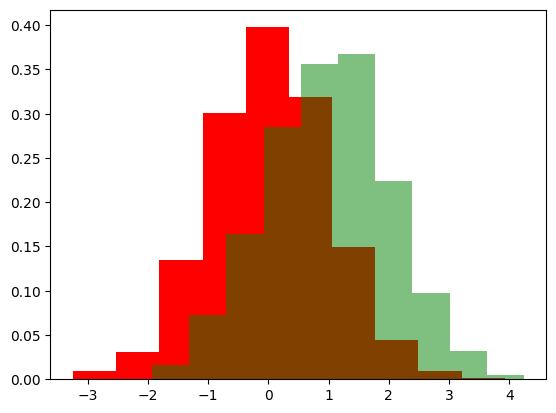
\includegraphics[width=\FigWidth]{figures/practice/chapter-3/sem4-cell10-out0.png}
\caption{Семинар~4: распределение $p$-value. На графике виден избыток малых $p$ слева.}
\label{fig:p3-pval}
\end{figure}
\textbf{Числа.} Без поправки отклоняют $\approx 50$ гипотез; ложных среди $H_0$ $\approx 7$--8 (ожидание $m_0\alpha\approx 7{,}5$).
\medskip\noindent\textbf{Три вопроса.} \textit{Постановка:} $m$ одновременных $t$-тестов. 
\textit{Применимость:} наивный порог $p<\alpha$ --- только иллюстрация; для отчёта нужна поправка. 
\textit{Вывод:} часть «значимостей» --- шум при множественности.\medskip

\paragraph{С поправкой.}
См. табл.~\ref{tab:model-mht} и пороги на рис.~\ref{fig:p3-thresh}: Holm/Bonferroni не допускают ложных среди $H_0$; BH --- компромисс FDR.
\begin{figure}[htbp]
\centering
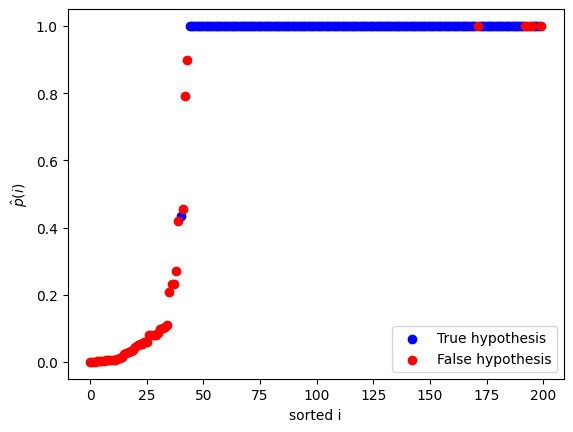
\includegraphics[width=\FigWidth]{figures/practice/chapter-3/sem4-cell27-out0.png}
\caption{Семинар~4: пороги Holm и BH. Обратите внимание, что BH отсекает больше малых $p$, чем строгий FWER.}
\label{fig:p3-thresh}
\end{figure}
\medskip\noindent\textbf{Три вопроса.} \textit{Постановка:} то же семейство из $m$ тестов. 
\textit{Применимость:} Holm при высокой цене ложной находки; BH при списке кандидатов. 
\textit{Вывод:} сообщить метод, число отклонений и смысл FDR.\medskip

\paragraph{Классификаторы (\S\ref{sec:examples}).}
Сравнение AUC на $m=14$ наборах: без поправки легко «найти» победу на iris; после Holm/BH устойчивых побед меньше --- тот же cherry-picking, что в таблице теории.
\medskip\noindent\textbf{Три вопроса.} \textit{Постановка:} $m$ парных сравнений алгоритмов. 
\textit{Применимость:} поправка на семейство до выбора «лучшего» датасета. 
\textit{Вывод:} одна строка таблицы AUC не лицензирует внедрение в прод.\medskip

По итогам: $m$, $\alpha$, метод, ложные без поправки, цена FWER, смысл BH.

\section{Контрольные вопросы по теме}

\begin{enumerate}
    \item При $m=100$ и $\alpha=0{,}05$ оцените вероятность хотя бы
          одной ошибки I рода без поправки, если все $H_i$ истинны и тесты независимы.
    \item Сформулируйте метод Холма для $m=4$ и порога $\alpha=0{,}05$
          с p-value $(0{,}001,\ 0{,}03,\ 0{,}04,\ 0{,}08)$.
          Сколько гипотез будет отвергнуто?
    \item Чем восходящая процедура BH принципиально отличается
          от нисходящей процедуры Холма?
    \item Почему $\FDR\leq\FWER$ для любой процедуры? Приведите
          содержательный пример, когда FDR-процедура предпочтительнее.
    \item Для дифференциальной экспрессии объясните, почему число
          отвержений BH ($8$) превышает число отклонений Холма ($4$).
    \item Сравните уровни значимости Холма и BH при $m=10$, $\alpha=0{,}05$.
          Сколько гипотез отвергнёт каждая процедура при p-value $(0{,}001,\ 0{,}02,\ 0{,}03,\ 0{,}04,\ 0{,}05,\ 0{,}06,\ 0{,}1,\ 0{,}2,\ 0{,}5,\ 0{,}8)$?
    \item Чем процедура BY отличается от BH? Когда BY предпочтительнее?
    \item Объясните, почему $q$-значение удобнее сырого p-value при
          скрининге $5000$ генов.
    \item Почему анализ $50$ подгрупп без поправки напоминает
          переобучение?
    \item Верно ли, что «p-value $=0{,}03$ означает, что $H_0$ верна с вероятностью 3\%»? Объясните.
    \item Сравните поправки Бонферрони и Шидака. При каких условиях Шидак менее консервативен?
    \item Чем FDP отличается от FDR? Почему cherry-picking без поправки не контролирует ни FWER, ни FDR?
\end{enumerate}

\chapter{Корреляция, таблицы сопряжённости и дисперсионный анализ}
\label{ch:anova}

Главы~\ref{ch:basics}--\ref{ch:multiple} посвящены сравнению распределений и контролю ошибок при множественных тестах.
Настоящая глава переходит к структуре зависимостей между признаками и к моделям с факторами, разбивающими выборку на группы.
Если в главе~\ref{ch:hypothesis} мы спрашивали, отличаются ли средние, то здесь добавляется вопрос о силе связи признаков и о том, как несколько факторов совместно объясняют отклик.

В \S\ref{sec:dependencies} рассматриваются связи между непрерывными и категориальными переменными~--- корреляция Пирсона и Спирмена, критерий $\chi^2$ для таблиц сопряжённости.
В \S\ref{sec:anova} вводится дисперсионный анализ (ANOVA) \citep{fisher1925}~--- однофакторный, двухфакторный и модель с повторными измерениями (within-subjects).
Методы ANOVA тесно связаны с линейной регрессией (глава~\ref{ch:regression}). F-критерий для групповых средних~--- частный случай проверки коэффициентов в модели с dummy-переменными. Понимание разложения суммы квадратов облегчит переход к множественной регрессии.

\section{Зависимости между признаками}
\label{sec:dependencies}

\begin{definition}
Коэффициент корреляции Пирсона $r_{X_1X_2}$ измеряет силу линейной связи: \[ r_{X_1X_2}=\frac{\cov(X_1,X_2)}{\sqrt{\mathbb DX_1\,\mathbb DX_2}}.
\] Выборочный аналог $\hat r$ вычисляется по парам $(X_{1i},X_{2i})$.
\end{definition}

Корреляция отвечает на вопрос о совместной изменчивости. Если $X_1$ превышает своё среднее, насколько предсказуемо $X_2$ окажется больше или меньше своего.
Пирсон естественен при примерной нормальности и линейной связи. В главе~\ref{ch:basics} мы уже видели, что оценка моментов чувствительна к выбросам, и корреляция наследует эту чувствительность.

Критерий Стьюдента для $r$ (связанные выборки, $(X_1,X_2)\sim N(\mu,\Sigma)$): \[ H_0\colon \rho=0,\qquad T=\frac{\hat r\sqrt{n-2}}{\sqrt{1-\hat r^2}}\sim St(n-2).
\] Корреляция Спирмена~--- коэффициент Пирсона для рангов. Устойчива к монотонным нелинейным связям и выбросам.
Выборочная формула через ранги $X_{1i}$, $X_{2i}$: \[ \hat\rho_{X_1X_2}=1-\frac{6}{n^3-n}\sum_{i=1}^n \bigl(\rank(X_{1i})-\rank(X_{2i})\bigr)^2.
\] Критерий Стьюдента для $H_0\colon\rho=0$ имеет тот же вид, что и для Пирсона, с $\hat\rho$ вместо $\hat r$.
Когда связь монотонна, но нелинейна (например, экспоненциальная), Спирмен часто обнаруживает зависимость там, где $\hat r\approx 0$.

Корреляция Кендалла $\tau$~--- доля согласованных пар минус доля несогласованных: \[ \hat\tau_{X_1X_2}=\frac{C-D}{C+D}, \] где $C$~--- число пар $(i,j)$ с одинаковым порядком $(X_{1i},X_{2i})$ и $(X_{1j},X_{2j})$, $D$~--- с разным.
При $H_0$ и $n>10$ используют нормальную аппроксимацию. $\hat\tau$ обычно меньше $|\hat\rho|$ по модулю, но устойчивее к большим разрывам рангов и точнее на малых $n$.
При нормальности $\mathbb E\hat\tau=\mathbb E\hat\rho= \frac{2}{\pi}\arcsin r$ асимптотически.

Преобразование Фишера для построения доверительного интервала для $\rho$. $z=\operatorname{arctanh}(\hat r)$ асимптотически нормально с дисперсией $1/(n-3)$.
Корреляция не подразумевает причинно-следственной связи. Высокий $r$ может быть следствием общего скрытого фактора или совпадения.
Пирсон чувствителен к выбросам и обнаруживает преимущественно линейные зависимости. При U-образной связи $\hat r\approx 0$ при сильной функциональной зависимости.
Перед формальным тестом $H_0\colon\rho=0$ разумно построить диаграмму рассеяния. Глаз часто замечает нелинейность и выбросы раньше, чем один числовой коэффициент их скроет.
Две переменные с U-образной связью дадут $\hat r\approx 0$ и незначимый t-тест, тогда как Спирмена или квадратичная регрессия (гл.~\ref{ch:regression}) обнаружат зависимость.
Корреляция~--- не универсальный детектор связи, а мера линейной совместной изменчивости.
Выбор между Пирсоном, Спирменом и Кендаллом~--- не формальность. При тяжёлых хвостах и монотонной, но нелинейной связи ранговые меры дают более надёжный тест $H_0\colon\rho=0$. При линейной нормальной зависимости Пирсон максимально эффективен.
На примере температуры и широты маргинально широта сильно связана с температурой. После учёта долготы частная связь ослабевает или меняет знак~--- тот же механизм, что контроль ковариат в ANOVA и регрессии (гл.~\ref{ch:regression}).
Перед публикацией $r=0{,}85$ всегда стоит проверить, не смешивает ли третий фактор два признака.

\begin{definition}
Частная корреляция $r_{X_1X_2|X_3}$ измеряет линейную связь $X_1$ и $X_2$ после учёта влияния $X_3$: \[ r_{X_1X_2|X_3}=\frac{r_{X_1X_2}-r_{X_1X_3}r_{X_2X_3}} {\sqrt{(1-r_{X_1X_3}^2)(1-r_{X_2X_3}^2)}}.
\] Для нескольких управляющих признаков $M$ используют обратную матрицу выборочных корреляций $R=\Omega^{-1}$: $r_{X_iX_j|M\setminus\{X_i,X_j\}}=-R_{ij}/\sqrt{R_{ii}R_{jj}}$.
\end{definition}

Проверка $H_0\colon r_{X_1X_2|X_3}=0$ при $(X_1,X_2,X_3)\sim N(\mu,\Sigma)$: \[ T=\frac{\hat r_{X_1X_2|X_3}\sqrt{n-M-2}} {\sqrt{1-\hat r_{X_1X_2|X_3}^2}}\sim St(n-M-2), \] где $M$~--- число управляющих признаков.

Множественная корреляция $R_{X,M}$ оценивает, какую долю дисперсии $X$ объясняют признаки из $M$ линейно. $R_{X,M}\in[0,1]$.
Высокая маргинальная корреляция может исчезнуть или усилиться после учёта третьего фактора.
Температура января в городах США сильно коррелирует с широтой ($r\approx -0{,}85$), слабо~--- с долготой. Частная корреляция температуры с долготой при фиксированной широте значима ($r\approx 0{,}28$), отражая континентальный климат.
Этот пример показывает, почему простая корреляция редко бывает окончательным ответом. Смешивающие переменные могут как маскировать, так и создавать ложное впечатление связи.
Частная корреляция~--- первый шаг к контролю ковариат, которую в главе~\ref{ch:regression} мы реализуем через включение предикторов в регрессионную модель. Формула через обратную корреляционную матрицу предвосхищает стандартизованные коэффициенты множественной регрессии.
На рис.~\ref{fig:correlation} показана диаграмма рассеяния двух непрерывных признаков с линией регрессии. Визуальная оценка предшествует формальному тесту $H_0\colon\rho=0$.

\begin{figure}[htbp]
    \centering
    
\includegraphics[width=\FigWidth]{\FigDir/chapter-4/corr_pearson.png}
    \caption{Диаграмма рассеяния и линейная регрессия.}
    \label{fig:correlation}
\end{figure}

Для таблицы $K_1\times K_2$ с частотами $n_{ij}$ и маргинальными суммами $n_{i+}$, $n_{+j}$, $n=\sum n_{ij}$: \[ H_0\colon \text{строка и столбец независимы},\qquad \chi^2=\sum_{i,j}\frac{\left(n_{ij}-\dfrac{n_{i+}n_{+j}}{n}\right)^2} {\dfrac{n_{i+}n_{+j}}{n}} =n\!\left(\sum_{i,j}\frac{n_{ij}^2}{n_{i+}n_{+j}}-1\right).
\] При $H_0$ и достаточных ожидаемых частотах ($\geq 5$ в большинстве ячеек) $\chi^2\sim\chi^2_{(K_1-1)(K_2-1)}$ асимптотически.
Условия~--- $n\geq 40$, ожидаемые частоты $<5$ не более чем в $20\%$ ячеек. Статистика измеряет отклонение наблюдаемых частот от ожидаемых при независимости. Большие значения указывают на систематическое совместное распределение категорий.

Точный критерий Фишера (таблица $2\times 2$). При фиксированных маргинальных суммах вероятность наблюдаемой таблицы \[ P=\frac{(a+b)!(c+d)!(a+c)!(b+d)!}{a!\,b!\,c!\,d!\,n!}.
\] p-value~--- сумма $P$ по всем таблицам с теми же суммами по строкам и столбцам, не более вероятных, чем наблюдаемая (двусторонний тест).
Для односторонней альтернативы $ad\ll bc$: \[ p=\sum_{i=0}^{a}\frac{C_{a+b}^{i}\,C_{c+d}^{a+c-i}}{C_n^{a+c}}.
\] На малых выборках асимптотический $\chi^2$ может быть ненадёжен. Точный критерий Фишера~--- стандартный выбор для таблиц $2\times 2$.
Для таблиц большего размера при нарушении условий на ожидаемые частоты используют точные перестановочные тесты или симуляцию. В прикладных пакетах (R, Python) выбор между асимптотическим и точным тестом обычно делается автоматически по правилам на минимальные ожидания.

\begin{definition}
Коэффициент $\phi$ (таблица $2\times 2$): $\phi=\sqrt{\chi^2/n}\in[-1,1]$.
Коэффициент V Крамера (общая $K_1\times K_2$): \[ V=\sqrt{\frac{\chi^2}{n\bigl(\min(K_1,K_2)-1\bigr)}}\in[0,1].
\] Нулевое значение~--- отсутствие связи. $V=1$~--- полное совпадение категорий (с точностью до переименования уровней).
\end{definition}

Корреляция Мэтьюса (бинарные признаки): $MCC=(ad-bc)/\sqrt{(a+b)(a+c)(b+d)(c+d)}$.
Значимый $\chi^2$ при большом $n$ не означает сильную связь. Коэффициенты $\phi$, $V$ и MCC измеряют силу ассоциации и должны сообщаться вместе с p-value, по аналогии с тем, как в главе~\ref{ch:hypothesis} важны не только значимость, но и величина эффекта.

Пример. Таблица образование~--- вера задаёт сопряжённость уровня образования (строки) и ответа на вопрос о религии (столбцы).
Критерий $\chi^2$ даёт $\chi^2\approx 76{,}1$, p-value $\ll 0{,}001$, степени свободы $(3-1)(6-1)=10$.

Распределение ответов зависит от образования. Например, доля ответа know God exists снижается с ростом образовательного уровня.
Остатки $(O-E)/\sqrt E$ показывают, какие ячейки вносят наибольший вклад в статистику.
Анализ остатков превращает глобальное отклонение от независимости в локальные содержательные утверждения о конкретных подгруппах.

Парадокс Симпсона. Разделим данные о лечении препаратом и плацебо по полу.
У мужчин препарат выигрывает ($\chi^2\approx 5{,}5$, p-value $\approx 0{,}02$), у женщин~--- тоже ($\chi^2\approx 17{,}6$, p-value $\ll 0{,}001$), но в объединённой таблице связи нет ($\chi^2\approx 0{,}4$, p-value $\approx 0{,}54$).
Препарат чаще давали мужчинам с тяжёлым течением, плацебо~--- женщинам с лёгким. Смешение пропорций переворачивает вывод.

Классический пример Беркли (1973). На уровне университета в целом мужчины поступали чаще женщин ($44{,}3\%$ против $34{,}6\%$, $\chi^2\approx 108$), но на каждом из крупнейших факультетов доля поступивших женщин не уступала мужчинам~--- женщины чаще подавали документы на конкурентные направления.
Содержательный вывод возможен только при согласованном разбиении или явном моделировании смешивающих факторов.
Парадокс Симпсона напоминает о роли частной корреляции. Маргинальная ассоциация может исчезнуть или сменить знак после учёта смешивающей переменной.
В прикладных исследованиях (медицина, социология, A/B-тестирование) таблицы сопряжённости часто сопровождают стратификацией по полу, возрасту или каналу трафика~--- именно чтобы не попасть в ловушку агрегированного вывода.
Пример лечения по полу с объединённой таблицей повторяет логику парадокса Симпсона на языке $\chi^2$. Значимость в подгруппах и отсутствие связи в агрегате~--- не противоречие формул, а следствие разных смешивающих пропорций.
Практический вывод~--- сначала стратификация по содержательным факторам, затем маргинальный тест, только если граф или предметная область оправдывает объединение.

При интерпретации таблиц сопряжённости следует избегать типичных ошибок.
\begin{itemize}
    \item Интерпретировать значимый $\chi^2$ как сильную связь.
          Для больших $n$ слабые отклонения от независимости значимы. Коэффициенты $\phi$, Cramér's $V$ измеряют силу связи.
    \item Применять асимптотический $\chi^2$ при малых ожидаемых
          частотах ($<5$) без точного критерия Фишера.
    \item Делать причинные выводы из таблицы сопряжённости
          без экспериментального дизайна.
\end{itemize}

\section{Дисперсионный анализ}
\label{sec:anova}

ANOVA разбивает общую вариабельность отклика на компоненты, обусловленные факторами и остаточную, и проверяет гипотезы о равенстве средних в группах при предположении нормальности и равенства дисперсий внутри групп.
Идея близка к $t$-критерию из главы~\ref{ch:hypothesis}. При двух группах однофакторный ANOVA эквивалентен двухвыборочному $t$-критерию, но при $K>2$ нужен единый общий критерий, прежде чем локализовать различия между парами.

Пусть $K$ групп, $n_k$ наблюдений в группе $k$, всего $N=\sum n_k$.
Разложение суммы квадратов: \[ \sum_{k,i}(Y_{ki}-\bar Y)^2= \underbrace{\sum_{k,i}(Y_{ki}-\bar Y_k)^2}_{\mathrm{SSW}}+ \underbrace{\sum_k n_k(\bar Y_k-\bar Y)^2}_{\mathrm{SSB}}, \] $\mathrm{SST}=\mathrm{SSW}+\mathrm{SSB}$.
Средние квадраты: $\mathrm{MSB}=\mathrm{SSB}/(K-1)$, $\mathrm{MSW}=\mathrm{SSW}/(N-K)$.
\[ H_0\colon \mu_1=\cdots=\mu_K,\qquad F=\frac{\mathrm{MSB}}{\mathrm{MSW}}\sim F(K-1,N-K)\ \text{при}\ H_0.
\] Межгрупповая сумма квадратов $\mathrm{SSB}$ отражает, насколько средние групп разбросаны вокруг общего среднего. Внутригрупповая $\mathrm{SSW}$~--- шум внутри групп. Большой $F$ означает, что междугрупповая вариация доминирует над внутригрупповой.
Предпосылки ANOVA~--- нормальность внутри групп и равенство дисперсий (гомоскедастичность)~--- проверяют до интерпретации. При их нарушении F-критерий может сохранять уровень значимости при больших $N$, но мощность и интервалы для разностей средних страдают.
Перед ANOVA имеет смысл построить ящики с усами по группам и проверить равенство дисперсий (Левена, F на $\sigma^2$). Нарушение гомоскедастичности при разных $n_k$ особенно опасно. F-тест может оставаться значимым, хотя различие средних объясняется смешением разброса и центра.
Робастная альтернатива~--- Крускала--Уоллиса с последующим апостериорным анализом по рангам.

\begin{definition}
Eta-squared (доля объяснённой дисперсии в выборке): $\eta^2=\mathrm{SSB}/\mathrm{SST}$.
Omega-squared (несмещённая оценка в популяции): \[ \hat\omega^2=\frac{\mathrm{SSB}-\mathrm{MSW}(K-1)} {\mathrm{SST}+\mathrm{MSW}/(N-K)}.
\] При отвержении $H_0$ важно сообщать не только p-value, но и $\eta^2$ или $\hat\omega^2$. При больших $N$ слабый эффект может быть статистически значимым.
\end{definition}

Критерий Крускала--Уоллиса (непараметрический общий). Ранжируем все $N$ наблюдений, $H_0\colon$ распределения в группах совпадают с точностью до сдвига. Без связок: \[ K=\frac{12}{N(N+1)}\sum_{k=1}^K n_k\bar r_k^2-3(N+1) \;\dot\sim\;\chi^2_{K-1}\quad (n_k>5).
\] HSD Тьюки (апостериорный, контролирует FWER попарных сравнений): \[ \mathrm{HSD}=\frac{q_\alpha(N-K)\,S}{\sqrt{\bar n}}, \quad S^2=\frac{\mathrm{SSW}}{N-K}, \quad \bar n=\frac{K}{\sum_k 1/n_k}.
\] Если $|\bar Y_i-\bar Y_j|>\mathrm{HSD}$, то $H_0\colon\mu_i=\mu_j$ отвергается. Ранговый аналог~--- критерий Неменьи.
При нарушении нормальности при больших $n$ F-критерий устойчив (robust). При неравных дисперсиях и разных $n_k$ предпочтителен критерий Уэлча или непараметрический Крускала--Уоллиса.
ANOVA проверяет наличие различий. Апостериорные тесты (HSD Тьюки) локализуют пары групп.
Связь с главой~\ref{ch:multiple} прямая. При $K$ группах попарных сравнений $K(K-1)/2$, и HSD Тьюки~--- один из способов контроля FWER без процедуры всех попарных $t$-тестов подряд.

Пример. В классическом примере ToothGrowth ($N=60$) измерена длина роста зубов (\texttt{len}) у крыс при двух типах добавки (\texttt{supp}: OJ, VC) и трёх дозах витамина~C (\texttt{dose}: 0.5, 1.0, 2.0).

На рис.~\ref{fig:anova-box} показаны ящики с усами по комбинациям факторов.
Однофакторный ANOVA по \texttt{supp} выявляет различие средних (p-value $\ll 0{,}001$). Апельсиновый сок (OJ) в среднем эффективнее аскорбата (VC).
По \texttt{dose} эффект дозы также значим. Рост увеличивается с дозой.
После значимого общего критерия HSD Тьюки локализует различия. Например, OJ превосходит VC, доза $2{,}0$~--- $0{,}5$ и $1{,}0$.
Ящики с усами помогают до формального теста увидеть, совпадают ли дисперсии и нет ли выбросов, нарушающих предпосылки ANOVA.
Класс ToothGrowth часто используют в учебных целях именно потому, что факторы \texttt{supp} и \texttt{dose} наглядны, а число наблюдений достаточно для устойчивого F-теста, но невелико~--- студент может наглядно увидеть различие между общим критерием и апостериорной локализацией.
Однофакторный ANOVA по \texttt{dose} отвечает на вопрос, есть ли эффект дозы вообще. HSD Тьюки отвечает, какие пары доз различаются.
Значимый общий критерий без апостериорного анализа лишь констатирует наличие различий.
Значимый апостериорный анализ при незначимом общем критерии при $K=2$ эквивалентен одному $t$-тесту. При $K>2$ он невозможен без предварительного F-теста (контроль FWER).

\begin{figure}[htbp]
    \centering
    
\includegraphics[width=\FigWidth]{\FigDir/chapter-4/drugs.png}
    \caption{Рост зубов по типу добавки и дозе витамина~C.}
    \label{fig:anova-box}
\end{figure}

Для факторов $A$ ($I$ уровней) и $B$ ($J$ уровней), по $n$ наблюдений в ячейке: \[ Y_{ijk}=\mu+\alpha_i+\beta_j+(\alpha\beta)_{ij}+\varepsilon_{ijk}, \quad \varepsilon_{ijk}\sim N(0,\sigma^2).
\] Разложение дисперсии (сбалансированный дизайн): \[ \mathrm{SS}_{total}=\mathrm{SS}_A+\mathrm{SS}_B+\mathrm{SS}_{AB}+\mathrm{SS}_{res}, \] \[ \mathrm{SS}_A=nJ\sum_i(\bar Y_{i\bullet}-\bar Y)^2,\quad \mathrm{SS}_B=nI\sum_j(\bar Y_{\bullet j}-\bar Y)^2, \] \[ \mathrm{SS}_{AB}=n\sum_{i,j} (\bar Y_{ij}-\bar Y_{i\bullet}-\bar Y_{\bullet j}+\bar Y)^2.
\] F-статистики: $F_A=\mathrm{MS}_A/\mathrm{MS}_{res}$, $F_B=\mathrm{MS}_B/\mathrm{MS}_{res}$, $F_{AB}=\mathrm{MS}_{AB}/\mathrm{MS}_{res}$.
Член $(\alpha\beta)_{ij}$ описывает взаимодействие. Эффект одного фактора зависит от уровня другого.
Интерпретировать main effects при значимом $A\times B$ без осторожности нельзя. Средний эффект фактора может не представлять ни одной реальной комбинации уровней.
Двухфакторный дизайн ToothGrowth естественно расширяется до модели с \texttt{supp}, \texttt{dose} и их произведением. Именно взаимодействие может объяснить, почему OJ эффективнее VC на одних дозах и нет на других, если такая картина видна на рис.~\ref{fig:anova-box}.

Пример. В данных об артериальном давлении измерено артериальное давление (\texttt{pressure}) при комбинациях биологической обратной связи (\texttt{biofeedback}: present/absent), диеты (\texttt{diet}) и препарата (\texttt{drug}: 1, 2, 3).

Двухфакторный ANOVA (biofeedback $\times$ diet) внутри \texttt{drug=1} даёт значимый эффект biofeedback ($F\approx 5{,}9$, p-value $\approx 0{,}024$). Присутствие обратной связи снижает давление.
Для \texttt{drug=2} эффект не значим (p-value $\approx 0{,}44$), что иллюстрирует взаимодействие препарата с не медицинским вмешательством.
Раздельный анализ по уровням \texttt{drug} здесь не прихоть, а содержательная необходимость. Объединённый ANOVA смешал бы разные механизмы действия препаратов.
Интуиция взаимодействия $A\times B$. Эффект фактора $A$ измеряется по-разному на разных уровнях $B$.
На графике \texttt{supp} $\times$ \texttt{dose} линии для OJ и VC могут пересекаться~--- тогда main effect \texttt{supp} без учёта взаимодействия вводит в заблуждение. Утверждение, что в среднем OJ лучше, не описывает ни одну конкретную дозу.
Такой график~--- обязательное дополнение к таблице F-тестов.

Within-subjects (повторные измерения). Один и тот же объект наблюдается во всех уровнях фактора $A$.
Модель: \[ Y_{ij}=\mu+\alpha_i+\gamma_j+\varepsilon_{ij}, \] где $\gamma_j$~--- эффект объекта $j$, $\sum\alpha_i=0$.
Разложение: \[ \mathrm{SS}_{total}=\mathrm{SS}_A+\mathrm{SS}_{subj}+\mathrm{SS}_{err}, \] \[ F=\frac{\mathrm{SS}_A/(K-1)} {(\mathrm{SS}_{wg}-\mathrm{SS}_{subj})/\bigl((n-1)(K-1)\bigr)} \sim F\bigl(K-1,(n-1)(K-1)\bigr)\ \text{при}\ H_0, \] где $\mathrm{SS}_{wg}$~--- общая внутрисубъектная вариабельность, $\mathrm{SS}_{subj}=K\sum_j(\bar Y_{\cdot j}-\bar Y)^2$~--- между субъектами.
Сферичность (Mauchly). Для $K>2$ все попарные разности $Y_{ik}-Y_{il}$ имеют одинаковую дисперсию при любом $i$.
Нарушение сферичности завышает вероятность ошибки I рода.
Поправки. Greenhouse--Geisser и Huynh--Feldt умножают числитель и знаменатель $F$ на коэффициент $\varepsilon\in(0,1]$, оцениваемый по ковариационной матрице. $\varepsilon=1$ при сферичности.
При сильном нарушении используют критерий Фридмана (ранговый общий) или multivariate подход.
Повторные измерения повышают мощность за счёт контроля межиндивидуальной вариабельности, но требуют выполнения сферичности ковариационной матрицы (критерий Mauchly).
При нарушении сферичности применяют поправки Greenhouse--Geisser или Huynh--Feldt. При $K=2$ сферичность выполняется автоматически.
Содержательно мы сравниваем изменение отклика у одних и тех же субъектов, а не смешиваем межиндивидуальные различия с эффектом условия.
Repeated-measures ANOVA~--- частный случай смешанной модели (глава~\ref{ch:regression}). Фиксированный эффект условия и случайный эффект субъекта разделяют два источника вариабельности, что особенно ценно, когда межсубъектный разброс велик (как в экспериментах с временем реакции).

Пример. Таблица данных о времени реакции на каннабис содержит время реакции ($\mu$с) для $12$ испытуемых при трёх условиях. Без воздействия (\texttt{None}), лёгком (\texttt{Light}) и умеренном (\texttt{Moderate}) употреблении марихуаны (столбцы). Строки~--- субъекты.

Это классическая схема repeated measures. Каждый испытуемый измерен трижды.
Однофакторный ANOVA с фактором условие и блоком субъект позволяет проверить $H_0\colon$ среднее время реакции не зависит от дозы, контролируя индивидуальные различия.
Профильные графики показывают рост времени реакции с дозой у большинства субъектов. При $K=3$ условиях имеет смысл проверить сферичность и при необходимости применить поправку G--G.
Ошибка~--- трактовать $36=12\times 3$ наблюдений как независимые. Это завышает мощность и искажает p-value, поскольку три измерения одного человека не независимы.
Парный подход из главы~\ref{ch:hypothesis} (критерий для разностей после минус до внутри субъекта) даёт эквивалент repeated-measures выводу при двух условиях. При $K>2$ нужна полная ANOVA-модель с блоком субъект.
Профиль до, лёгкое и умеренное у одного испытуемого~--- связанные наблюдения. Игнорирование субъекта эквивалентно завышению $n$ и занижению p-value.
Содержательно мы спрашиваем, меняется ли реакция внутри человека, а не отличаются ли 36 независимых измерений.
Repeated-measures ANOVA формализует этот вопрос через блок субъект и F-тест на эффект условия.

При планировании ANOVA следует помнить о типичных ловушках.
\begin{itemize}
    \item Применять однофакторный ANOVA к времени реакции без учёта
          субъекта, трактуя $36$ наблюдений как независимые~--- завышает мощность и искажает p-value.
    \item Игнорировать взаимодействие в гипертонии и
          интерпретировать main effects при значимом $A\times B$.
    \item Считать незначимый F-тест доказательством отсутствия эффекта
          без анализа мощности и доверительных интервалов для разностей.
\end{itemize}

Исследование связи между часами обучения ($X$) и баллом экзамена ($Y$) для $n=200$ студентов.
Диаграмма рассеяния показывает линейный тренд, $\hat r=0{,}52$, $t$-тест на $\rho=0$ даёт p-value $\ll 0{,}001$.
Известен фактор факультет (гуманитарный / технический). Частная корреляция $r_{XY|Z}$ падает до $0{,}21$~--- часть связи объясняется разным распределением часов по факультетам.

Параллельно однофакторный ANOVA балл по факультету ($K=3$ группы) даёт значимый $F$, $\eta^2=0{,}14$.
Апостериорный HSD локализует различие между гуманитарным и техническим.
Маргинальная корреляция часов и баллов завышена из-за смешивания групп. ANOVA и частная корреляция согласуются в том, что факультет~--- смешивающий фактор в регрессионном смысле (гл.~\ref{ch:regression}).

Если бы мы игнорировали $Z$ и строили только регрессию часов на балл, политика больше часов всем могла бы не работать внутри факультета.
Такой пример связывает \S~\ref{sec:dependencies} и \S~\ref{sec:anova}. Разные инструменты, один вопрос о структуре зависимостей.
График (диаграмму рассеяния с цветом по факультету) следует построить до любого из формальных тестов.

Прикладной отчёт часто смешивает типы переменных. Непрерывные предикторы (корреляция, регрессия), категориальные (таблицы $\chi^2$), групповые средние (ANOVA).
Ошибка~--- применить один тест по привычке. $\chi^2$ к дискретизированному непрерывному признаку без обоснования интервалов. ANOVA к парным данным без блока субъект. Корреляцию Пирсона к монотонной нелинейной связи.
Явная строка тип переменной и метод в начале анализа предотвращает такие подмены и связывает \S~\ref{sec:dependencies} и \S~\ref{sec:anova} в единую методологию.

Dummy-кодирование фактора с $K$ уровнями и однофакторный ANOVA эквивалентны линейной модели с $K-1$ индикаторами.
F-тест на все dummy~--- общий ANOVA. t-тест на один коэффициент~--- contrast.
Понимание ANOVA через регрессию (гл.~\ref{ch:regression}) снимает ощущение другого предмета. $\mathrm{SSB}$~--- объяснённая регрессией доля $TSS$ при групповых предикторах.
Two-way ANOVA с interaction соответствует модели с произведениями dummy.

Значимый общий F или $\chi^2$ при большом $n$ совместим с малым $\eta^2$ или Cramér's $V$.
В отчёте указывают p-value, меру силы ($\eta^2$, $\phi$, $d$ Коэна для контрастов), график (ящики, мозаичная диаграмма).
Апостериорный анализ только после значимого общего критерия (кроме запланированных контрастов).
Repeated measures требуют явно указать субъект в модели.

\section{G-критерий, перестановочная корреляция и робастный ANOVA}

G-критерий для таблиц сопряжённости. Логарифмическое отношение правдоподобия для независимости в таблице $K_1\times K_2$: \[ G^2 = 2\sum_{i,j} n_{ij}\ln\frac{n_{ij}n}{n_{i+}n_{+j}} = 2n\!\left(\sum_{i,j}\frac{n_{ij}}{n}\ln\frac{n_{ij}n}{n_{i+}n_{+j}}\right).
\] При $H_0$ и больших ожидаемых частотах $G^2\dot\sim\chi^2_{(K_1-1)(K_2-1)}$, как и статистика Пирсона $\chi^2$. Численно $G^2\approx\chi^2$.
G-критерий удобен в логлинейных и GLM-моделях (гл.~\ref{ch:regression}).

\begin{critcard}{G-критерий независимости}
Выборка & связанные $(X_{1i},X_{2i})$, $X_1\in\{1,\ldots,K_1\}$, $X_2\in\{1,\ldots,K_2\}$ \\
$H_0$ & $X_1$ и $X_2$ независимы \\
Статистика & $G^2 = 2\sum_{i,j} n_{ij}\ln\bigl(n_{ij}n/(n_{i+}n_{+j})\bigr)$ \\
Нулевое распр. & $\chi^2_{(K_1-1)(K_2-1)}$ (асимптотика) \\
p-value & хвост $\chi^2$; те же условия на ожидаемые частоты, что у $\chi^2$ Пирсона \\
\end{critcard}

Перестановочный критерий для корреляции $r$. Для связанных выборок $(X_{1i},X_{2i})$ при $H_0\colon\rho=0$ переставляют индексы одной из выборок ($n!$ вариантов).
На каждой перестановке $g$ вычисляют $\hat r(X_1^n, gX_2^n)$. p-value~--- доля перестановок с $|\hat r|\geq|\hat r_{\text{obs}}|$ (двусторонний тест).

\begin{critcard}{Перестановочный тест $H_0\colon\rho=0$}
Выборки & связанные $X_1^n$, $X_2^n$ \\
$H_0$ & $\rho=0$ (линейная корреляция Пирсона) \\
Статистика & $T=\hat r_{X_1X_2}$ \\
Нулевое распр. & эмпирическое по перестановкам $X_2^n$ \\
p-value & $\#\{g\colon|\hat r_g|\geq|\hat r_{\text{obs}}|\}/n!$ (или Монте-Карло) \\
\end{critcard}

Критерий Джонкхеера--Терпстра. Omnibus для упорядоченных групп. $H_0\colon F_1=\cdots=F_K$ против $H_1\colon F_1\preceq\cdots\preceq F_K$ (стохастический порядок).
Статистика $S=\sum_{k,i} a_{ki}$, где $a_{ki}$~--- число наблюдений в группах $1,\ldots,k-1$, меньших $X_{ki}$.
При $n_k>10$: $S\sim N(\mu,\sigma^2)$ с формулами $\mu,\sigma$ из лекции~6.

\begin{critcard}{Джонкхеер--Терпстра (тренд по группам)}
Выборки & $K$ независимых групп, размеры $n_k$ \\
$H_0$ & $\med X_1=\cdots=\med X_K$ (равные распределения) \\
$H_1$ & $\med X_1\leq\cdots\leq\med X_K$ (не все равны) \\
Статистика & $S=\sum_{k,i}a_{ki}$ (число меньших слева) \\
Нулевое распр. & табличное; нормальная аппроксимация при больших $n_k$ \\
\end{critcard}

Критерий Даннета. Сравнение $K-1$ лечений с одной контрольной группой (индекс~1): \[ D_i = \frac{\bar X_i-\bar X_1}{S\sqrt{1/n_i+1/n_1}},\quad S^2=\frac{1}{N-K}\sum_k (n_k-1)S_k^2.
\] При нормальности и $\mu_1=\cdots=\mu_K$ вектор $(D_2,\ldots,D_K)$ имеет многомерное $t$-распределение. Пороги дают FWER для семейства каждая группа против контроля.

\begin{critcard}{Даннет (все группы против контроля)}
Выборки & $K$ нормальных групп, общая $\sigma^2$ \\
$H_0$ & $\mu_1=\cdots=\mu_K$ \\
Частные $H_0^{(i)}$ & $\mu_i=\mu_1$, $i=2,\ldots,K$ \\
Статистика & $D_i$ как выше \\
Нулевое распр. & многомерное $t$ (таблицы Даннета) \\
Гарантия & контроль FWER для семейства сравнений с контролем \\
\end{critcard}

LSD Фишера. После значимого общего ANOVA попарно сравнивают \[ \frac{\bar X_i-\bar X_j}{S\sqrt{1/n_i+1/n_j}}\sim St(n_i+n_j-2).
\] Наименьшая значимая разность: \[ \mathrm{LSD}_{ij}=\frac{t_{\alpha,\,n_i+n_j-2}\,S}{\sqrt{1/n_i+1/n_j}}.
\] Если $|\bar X_i-\bar X_j|>\mathrm{LSD}_{ij}$, отвергают $H_0\colon\mu_i=\mu_j$.

\begin{remark}
LSD не контролирует FWER при множественных попарных сравнениях. Использовать только как исследовательский инструмент после $F$-теста, не как замену HSD Тьюки или Холма.
\end{remark}

Критерий Бартлетта (однородность дисперсий). Проверка $H_0\colon\sigma_1^2=\cdots=\sigma_K^2$ перед ANOVA: \[ B = \frac{\ln 10}{C}\left((N-K)\ln S^2 - \sum_k (n_k-1)\ln S_k^2\right), \quad C = 1+\frac{1}{3(K-1)}\left(\sum_k\frac{1}{n_k-1}-\frac{1}{N-K}\right), \] $S^2$~--- объединённая дисперсия. При $n_k>6$: $B\dot\sim\chi^2_{K-1}$.
Критерий чувствителен к ненормальности. При сомнениях~--- Левена.

\begin{critcard}{Бартлетт (гомогенность $\sigma^2$)}
Выборки & $X_{ki}\sim N(\mu_k,\sigma_k^2)$ \\
$H_0$ & $\sigma_1^2=\cdots=\sigma_K^2$ \\
Статистика & $B(X^N)$ как выше \\
Нулевое распр. & $\chi^2_{K-1}$ (аппроксимация) \\
\end{critcard}

Критерий Неменьи (CD). Ранговый апостериорный анализ после Крускала--Уоллиса. Критическая разность: \[ \mathrm{CD} = q'_\alpha\sqrt{\frac{K(K+1)}{6N}}, \] где $q'_\alpha$~--- квантиль стьюдентизированного размаха для рангов.
Если $|\bar r_i-\bar r_j|>\mathrm{CD}$, отвергают $H_0\colon$ сдвиг $i$-й и $j$-й групп совпадает.

\begin{critcard}{Неменьи (попарно по рангам)}
Предпосылка & значимый или плановый Крускала--Уоллиса \\
$H_0^{(ij)}$ & распределения в группах $i,j$ совпадают (по рангам) \\
Статистика & $|\bar r_i-\bar r_j|$ и $\mathrm{CD}$ \\
Гарантия & FWER для попарных сравнений в ранговой постановке \\
\end{critcard}

Критерии Фридмана и Пейджа (повторные измерения). Для $n$ субъектов и $K$ условий ранжируют отклик внутри каждой строки (субъекта). $r_{ki}$~--- ранг $k$-го условия у $i$-го субъекта, $R_k=\sum_i r_{ki}$.
\[ S = \frac{12}{nK(K+1)}\sum_{k=1}^K R_k^2 - 3n(K+1) \quad\text{(Фридман, общий)}.
\] Пейдж (тренд): $L=\sum_{k=1}^K k R_k$. При $H_0$ и больших $n,K$: $L\sim N(\mu_L,\sigma_L^2)$ с параметрами из лекции~6.

\begin{critcard}{Фридман (within-subjects, общий)}
Данные & матрица $X_{ki}$, $i=1,\ldots,n$, $k=1,\ldots,K$ \\
$H_0$ & $\alpha_1=\cdots=\alpha_K$ (эффект условия отсутствует) \\
Статистика & $S$ через ранги $r_{ki}$ в строках \\
Нулевое распр. & $\chi^2_{K-1}$ при $n>15$, $K>10$ \\
\end{critcard}

\begin{critcard}{Пейдж (тренд условий)}
$H_0$ & как у Фридмана \\
$H_1$ & $\alpha_1\leq\cdots\leq\alpha_K$ (монотонный тренд) \\
Статистика & $L=\sum_k k R_k$ \\
Нулевое распр. & $N(\mu_L,\sigma_L^2)$ (аппроксимация) \\
\end{critcard}

Критерий Крускала--Уоллиса (кратко). Ранговый общий для $K$ независимых групп (дополнение к \S~\ref{sec:anova}). Ранжировать все $N$ наблюдений, $\bar r_k$~--- средний ранг в группе $k$, \[ H = \frac{12}{N(N+1)}\sum_{k=1}^K n_k\bar r_k^2 - 3(N+1) \;\dot\sim\;\chi^2_{K-1}\quad (n_k>5).
\] После значимого $H$~--- апостериорный Неменьи. При упорядоченных уровнях фактора~--- Джонкхеер вместо $H$.

\begin{critcard}{Крускал--Уоллис}
Выборки & $K$ независимых групп, $N=\sum n_k$ \\
$H_0$ & распределения совпадают (сдвиг не отличается) \\
Статистика & $H$ (или $K$ в обозначениях лекции) через $\bar r_k$ \\
Нулевое распр. & $\chi^2_{K-1}$ \\
\end{critcard}

При сильной асимметрии или выбросах Крускала--Уоллиса заменяет F-тест. Попарные сравнения~--- по рангам (Немени).
Дисперсионный анализ Уэлча обобщает $t$-Уэлча на $K>2$ групп при неравных дисперсиях.
Выбор процедуры следует той же схеме, что в гл.~\ref{ch:hypothesis}. График, предпосылки, общий критерий, апостериорный анализ с поправкой.

\section{Практика и семинар}
\label{sec:practice-ch4}

Задания соответствуют семинарам~5--6. Для каждой задачи зафиксируйте тип переменных, $H_0/H_1$, предпосылки, числовой вывод (p-value, размер эффекта) и содержательную интерпретацию в 3--5 предложениях.

Корреляция и выброс (sem5). Модель $X_1\sim N(0,1)$, $X_2=X_1+\varepsilon$, $\varepsilon\sim N(0,\alpha^2)$, $n=10$ (затем $n=10^5$). Теоретически $r=1/\sqrt{1+\alpha^2}$.

Шаги.

\begin{enumerate}
    \item Сгенерировать пары. Вычислить $\hat r$, $t$-тест $H_0\colon\rho=0$
          и ДИ через преобразование Фишера. Сравнить с теорией.
    \item Для $\alpha\in\{0{,}1,0{,}5,\ldots,5\}$ (шум) в цикле $1000$ раз
          оценить долю принятий $H_0$ при истинном $r\neq 0$ (мощность/ошибка II рода для малых $n$).
    \item Выброс. При $n=10^5$, $\alpha=1$ добавить к одной точке
          сдвиг $+9999$ по $X_1$. Сравнить $\hat r$ Пирсона до/после. Повторить для Спирмена и Кендалла.
    \item Перестановочный тест. Для данных без выброса оценить
          $p_{\text{perm}}$ (перестановка $X_2$). Сравнить с $p_t$.
    \item Интерпретация. Объяснить, почему один выброс меняет
          вывод Пирсона, но почти не меняет ранговые коэффициенты. Когда перестановочный p-value заметно отличается от $t$.
\end{enumerate}

Гипертония. Трёхфакторный ANOVA (sem6). Данные.\texttt{biofeedback} $\times$ \texttt{diet} $\times$ \texttt{drug} $\to$ \texttt{pressure} ($N=72$, Maxwell \& Delaney).

Шаги.

\begin{enumerate}
    \item Построить ящики с усами по \texttt{drug} и фасетам
          \texttt{biofeedback}$\times$\texttt{diet}.
    \item Оценить трёхфакторную модель с взаимодействиями
          \texttt{drug*diet*biofeedback} (Type~II/III ANOVA).
    \item Если $A\times B\times C$ значимо~--- не интерпретировать
          main effects без графика. Разобрать простые эффекты (например, \texttt{biofeedback} внутри \texttt{drug=1}).
    \item Сопоставить с примером \S~\ref{sec:anova}. Почему отдельный ANOVA
          по уровням \texttt{drug} содержательно оправдан.
    \item Интерпретация. Сформулировать, какие комбинации лечения
          снижают давление. Указать $F$, p-value, $\eta^2$ для значимых членов.
\end{enumerate}

Хоровые певцы. Бартlett и Тьюки (sem6). Данные. Рост (дюймы) и регистр голоса (\texttt{voice}: bass, baritone, tenor, alto), $n=235$.

Шаги.

\begin{enumerate}
    \item Визуализация (ящики, violin plot).
    \item \texttt{scipy.stats.bartlett} по группам. $H_0\colon\sigma^2$
          одинаковы. При p-value $<0{,}05$~--- дисперсионный анализ Уэлча или Крускала--Уоллиса вместо классического $F$.
    \item Однофакторный ANOVA (или робастный аналог). При значимом общем критерии~---
          \texttt{pairwise\_tukeyhsd} / \texttt{multicomp}.
    \item Интерпретация. Есть ли систематическая связь роста
          с регистром? Указать, какие пары различаются по апостериорному анализу. Обсудить нарушение гомогенности дисперсий, если оно есть.
\end{enumerate}

Витамин~C и рост зубов морских свинок (sem6). Данные.\texttt{ToothGrowth}: \texttt{len}, \texttt{supp} (OJ/VC), \texttt{dose} (0.5, 1.0, 2.0).

Шаги.

\begin{enumerate}
    \item График \texttt{len} и \texttt{dose}, цвет по \texttt{supp}.
    \item Двухфакторный ANOVA \texttt{len ~ supp * dose}. Проверить
          взаимодействие на графике (параллельность линий).
    \item При значимом общем критерии по \texttt{dose}~--- HSD Тьюки для доз.
          Отдельно прокомментировать \texttt{supp}.
    \item Сравнить с табл.~лекции (HSD для жаропонижающих). Логика та же.
    \item Интерпретация. Какая добавка и доза максимальны.
          Есть ли пересечение кривых OJ/VC?
\end{enumerate}

Марихуана и время реакции (sem6). Данные $12$ субъектов $\times$ $3$ условия (\texttt{None}, \texttt{Light}, \texttt{Moderate}). Отклик~--- время реакции ($\mu$с).

Шаги.

\begin{enumerate}
    \item Профильный график. Субъект $\times$ условие (линии по испытуемым).
    \item Ошибка. Сравнить однофакторный ANOVA на $36$ точках
          без блока субъект с repeated-measures моделью (\texttt{AnovaRM} / mixed LM с случайным intercept).
    \item Проверить сферичность (Mauchly). При нарушении~--- поправка
          Greenhouse--Geisser.
    \item Апостериорный попарно (с поправкой) или контрасты доза и None.
    \item Интерпретация. Растёт ли время реакции с дозой?
          Почему $36$ наблюдений нельзя считать независимыми.
          Связь с \S~\ref{sec:anova} о дисперсионном анализе с повторными измерениями.
\end{enumerate}

\section{Контрольные вопросы по теме}

\begin{enumerate}
    \item Чем корреляция Пирсона отличается от Спирмена?
          Приведите пример нелинейной монотонной связи, где $\hat r_{\text{Пирсона}}\approx 0$, а $\hat r_{\text{Спирмена}}\neq 0$.
    \item Для таблицы образование--вера укажите число степеней свободы
          критерия $\chi^2$ и интерпретируйте результат в словах.
    \item Запишите разложение $Y_{ijk}=\mu+\alpha_i+\beta_j+(\alpha\beta)_{ij}+\varepsilon_{ijk}$
          для ToothGrowth. Какие факторы соответствуют \texttt{supp} и \texttt{dose}?
    \item Почему для гипертонии уместен отдельный ANOVA
          по каждому уровню \texttt{drug}?
    \item Объясните структуру времени реакции как repeated measures.
          Какой F-тест проверяет эффект условия?
    \item Сравните ANOVA и парный $t$-критерий при двух группах.
          Когда результаты совпадают?
    \item Почему корреляция между числом пожарных и ущербом от огня
          не доказывает, что пожарные «вызывают» ущерб?
    \item Вычислите $V$ Крамера для таблицы образование--вера
          при $\chi^2\approx 76{,}1$, $n$ известном из данных.
    \item Объясните парадокс Симпсона на примере лечения по полу.
    \item Запишите разложение $\mathrm{SST}=\mathrm{SSW}+\mathrm{SSB}$
          и интерпретируйте $\eta^2$ для ToothGrowth.
    \item Когда предпочтителен Крускал--Уоллис вместо F-критерия?
    \item Чем HSD Тьюки отличается от попарных $t$-критериев без поправки?
    \item Зачем при repeated measures проверять сферичность?
\end{enumerate}

\chapter{Линейная регрессия, диагностика и обобщённые линейные модели}
\label{ch:regression}

Главы~\ref{ch:basics}--\ref{ch:multiple} заложили аппарат распределений, доверительных интервалов и проверки гипотез. Мы научились спрашивать, отличается ли среднее двух групп и согласуются ли данные с $H_0$, опираясь на $t$-, $F$- и $\chi^2$-критерии при известных предпосылках.
Регрессионный анализ переносит эту логику на задачу описания зависимости. Как изменяется отклик $y$ при варьировании предикторов $x_1,\ldots,x_k$.
Вместо сравнения двух выборочных средних мы оцениваем параметры линейной (или обобщённой линейной) модели и проверяем, какие из них статистически значимы при заданном уровне $\alpha$.

Метод наименьших квадратов (МНК) даёт линейную аппроксимацию условного матожидания $\mathbb{E}(y\mid x)$ \citep{casella2002}. Обобщённые линейные модели (GLM) расширяют этот аппарат на бинарные и счётные отклики, где нормальность остатков уже неуместна, а связь между $\mathbb{E}(y\mid x)$ и $x^\top\beta$ задаётся через связующую функцию.
Без проверки предположений и содержательной интерпретации коэффициентов регрессия легко превращается в формальную подгонку чисел. $R^2$ растёт, p-value выглядят убедительно, а прогноз за пределами обучающей выборки оказывается бессмысленным.
Структура главы повторяет логику предыдущих. Сначала модель и оценивание, затем инференс (доверие к p-value при выполнении предпосылок), диагностика (проверка этих предпосылок) и обобщение на другие типы отклика.
Настоящая глава связывает оценивание, инференс и диагностику в единую цепочку. От постановки МНК через классические $t$- и $F$-тесты к проверке остатков и, наконец, к GLM для качественных и счётных данных.

\section{Постановка и метод наименьших квадратов}

Пусть $n$ объектов описываются матрицей предикторов $X\in\mathbb{R}^{n\times(k+1)}$ (первый столбец~--- единицы) и вектором отклика $y\in\mathbb{R}^n$.
Строка $x_i^\top$~--- признаки $i$-го объекта.
Интуитивно каждый $y_i$~--- реализация случайной величины с условным распределением, зависящим от $x_i$. Регрессия ищет простое правило, которое наилучшим образом предсказывает типичное значение $y_i$ при заданном $x_i$.

\begin{definition}
Линейная модель задаёт отклик как сумму линейной комбинации предикторов и случайной ошибки:
\[ y = X\beta + \varepsilon, \qquad \mathbb{E}(\varepsilon\mid X)=0.
\]
\end{definition}

\begin{definition}
Метод наименьших квадратов (МНК, OLS) минимизирует $\|y-X\beta\|_2^2$ и эквивалентен минимизации $\sum_i (y_i-\mathbb{E}(y_i\mid x_i))^2$ в классе линейных предикторов. Оценка $\hat\beta$ называется OLS-оценкой.
\end{definition}

Геометрически $\hat y=X\hat\beta$~--- ортогональная проекция $y$ на столбцовое пространство $X$. Остатки $y-\hat y$ перпендикулярны всем столбцам $X$, что и выражает условие первого порядка.
Условие первого порядка $2X^\top(y-X\beta)=0$ даёт нормальные уравнения $X^\top X\beta=X^\top y$ и при $\rank X=k+1$:
\[ \hat\beta = (X^\top X)^{-1}X^\top y, \qquad \hat y = Hy, \quad H=X(X^\top X)^{-1}X^\top.
\]
Матрица $H$ (hat matrix) проецирует $y$ на столбцовое пространство $X$. Диагональные элементы $h_{ii}$ измеряют рычаг $i$-го наблюдения~--- насколько сильно точка $(x_i,y_i)$ тянет подгонку к себе.
Следствие $H^2=H$. Повторная проекция не меняет результат. Сумма диагональных элементов $\sum_i h_{ii}=k+1$ связывает общий рычаг с числом параметров модели.

Разложение сумм квадратов $TSS=\sum(y_i-\bar y)^2$, $ESS=\sum(\hat y_i-\bar y)^2$, $RSS=\sum(y_i-\hat y_i)^2$, $TSS=ESS+RSS$.
Коэффициент детерминации $R^2=ESS/TSS=1-RSS/TSS$.
Приведённый $R^2_a$ $1-(1-R^2)\frac{n-1}{n-k-1}$~--- для сравнения моделей с разным числом регрессоров.
Следует помнить. Высокий $R^2$ не доказывает причинность и не гарантирует хороший прогноз на новых данных. Он лишь количественно описывает долю вариации $y$, объяснённую линейной комбинацией $x$ на данной выборке \citep{casella2002}.

\begin{definition}
(1)~линейность $y=X\beta+\varepsilon$. (2)~случайная выборка. $(x_i,y_i)$ независимы. (3)~полный ранг $\rank X=k+1$. (4)~$\mathbb{E}(\varepsilon\mid X)=0$. (5)~гомоскедастичность $\mathbb{D}(\varepsilon\mid X)=\sigma^2 I$.
При их выполнении МНК-оценки $\hat\beta$ несмещены, состоятельны и имеют наименьшую дисперсию среди линейных по $y$ несмещённых оценок (теорема Гаусса--Маркова).
\end{definition}

Предположения (2) и (4) связывают регрессию с i.i.d.-посылкой глав~1--2. Нарушение независимости (например, временные ряды или кластеры) требует робастных или специализированных процедур, которые мы затронем кратко и подробно разберём в гл.~\ref{ch:timeseries}.

Эскиз доказательства теоремы Гаусса--Маркова. Пусть $\tilde\beta=Ay$~--- произвольная линейная несмещённая оценка $\beta$ ($A$ не зависит от $y$, $AX=I_{k+1}$).
Тогда $\tilde\beta-\hat\beta=(A-(X^\top X)^{-1}X^\top)y$ не зависит от истинного $\beta$, а при $\mathbb{E}(\varepsilon\mid X)=0$ и $\mathbb{D}(\varepsilon\mid X)=\sigma^2 I$:
\[ \cov(\tilde\beta-\hat\beta\mid X) =\sigma^2\bigl(A-(X^\top X)^{-1}X^\top\bigr) \bigl(A-(X^\top X)^{-1}X^\top\bigr)^\top.
\]
Матрица $\cov(\hat\beta\mid X)=\sigma^2(X^\top X)^{-1}$.
Разность ковариаций $\cov(\tilde\beta\mid X)-\cov(\hat\beta\mid X)$ положительно полуопределена. Это следует из тождества $(A-(X^\top X)^{-1}X^\top)X=0$ и разложения $\cov(\tilde\beta\mid X)=\cov(\tilde\beta-\hat\beta\mid X)+\cov(\hat\beta\mid X)$.
Значит, $\hat\beta$ оптимален в классе линейных несмещённых оценок.
Замечание. Нелинейные или смещённые оценки (ridge, lasso) могут дать меньшую среднеквадратичную ошибку при мультиколлинеарности.
В терминах гл.~\ref{ch:basics} теорема отвечает на вопрос, какую линейную оценку выбрать, но не на вопрос, верна ли линейная модель вообще. Для этого нужна диагностика остатков.
Теорема не утверждает, что МНК~--- лучший метод вообще. Она ограничивает класс сравнения линейными несмещёнными оценками, что согласуется с частотной логикой глав~1--2, где мы ищем процедуры с контролируемым уровнем ошибки I рода при корректных предпосылках.

Дисперсия $\hat\beta_j$ растёт с $\sigma^2$ и мультиколлинеарностью $x_j$:
\[ \mathbb{D}(\hat\beta_j\mid X)=\frac{\sigma^2}{\mathrm{TSS}_j(1-R_j^2)}, \]
где $R_j^2$~--- $R^2$ регрессии $x_j$ на остальные столбцы $X$, $\mathrm{TSS}_j=\sum_i(x_{ij}-\bar x_j)^2$.
В матричной форме $\mathbb{D}(\hat\beta\mid X)=\sigma^2(X^\top X)^{-1}$. Почти линейно зависимые столбцы делают $X^\top X$ плохо обусловленной, и малые изменения $y$ могут сильно сдвигать $\hat\beta$. Это не ошибка метода, а сигнал о недостатке информации в данных.

VIF (variance inflation factor) для $j$-го предиктора:
\[ \mathrm{VIF}_j=\frac{1}{1-R_j^2}.
\]
$\mathrm{VIF}_j>10$ (иногда $>5$) сигнализирует о сильной мультиколлинеарности. Доверительные интервалы для $\beta_j$ расширяются примерно в $\sqrt{\mathrm{VIF}_j}$ раз. Лечение~--- отбор признаков, центрирование, регуляризация или содержательное объединение коррелированных факторов.
Важно не путать статистическую и содержательную проблему. Высокий VIF не доказывает, что один из предикторов лишний с точки зрения причинности, но предупреждает, что отдельные $t$-тесты для коэффициентов могут быть нестабильны при малом сдвиге данных.

Пример. Внешность и оценка курса. В исследовании красота и оценка курса измерены внешность преподавателя (\texttt{looks}) и итоговую оценку курса (\texttt{course\_eval}).
Простая линейная регрессия показывает положительную связь. На каждую единицу прироста \texttt{looks} ожидается изменение $\hat\beta_1$ баллов оценки при прочих равных (здесь других предикторов нет).
Интерпретация при прочих равных имеет смысл только в рамках линейной модели и при отсутствии смешивающих факторов, не включённых в $X$.
Даже при значимом $\hat\beta_1$ нельзя автоматически заключать причинность. Внешность может коррелировать с другими характеристиками преподавателя, не измеренными в данных.
График остатков (рис.~\ref{fig:reg-residuals}) позволяет проверить линейность и гомоскедастичность~--- первый шаг диагностики, без которого $t$- и $F$-критерии следующего раздела теряют обоснованность.

\begin{figure}[htbp]
    \centering
    
\includegraphics[width=\FigWidth]{\FigDir/chapter-5/goodres.png}
    \caption{OLS-подгонка и остатки (иллюстрация на синтетических данных).}
    \label{fig:reg-residuals}
\end{figure}

\section{Инференс в линейной модели}

При нормальности ошибок $\varepsilon\sim N(0,\sigma^2 I)$ (шестое предположение) МНК совпадает с МП. $\hat\beta\sim N(\beta,\sigma^2(X^\top X)^{-1})$, $\hat\sigma^2=RSS/(n-k-1)$, $(n-k-1)\hat\sigma^2/\sigma^2\sim\chi^2_{n-k-1}$.
Шестое предположение не входит в теорему Гаусса--Маркова, но необходимо для точных (не только асимптотических) интервалов и p-value в конечных выборках~--- ровно так же, как $t$-критерий в гл.~\ref{ch:basics} опирается на нормальность при малых $n$.
При больших $n$ центральная предельная теорема оправдывает асимптотические интервалы даже при умеренном отклонении от нормальности ошибок, но на малых выборках и при тяжёлых хвостах $y$ Q--Q график остатков остаётся обязательным.
Оценка $\hat\sigma^2=RSS/(n-k-1)$ несмещена при гомоскедастичности. Подстановка в $t$-статистику даёт распределение Стьюдента с $n-k-1$ степенями свободы~--- прямой аналог одновыборочного $t$-критерия, но для линейной комбинации коэффициентов $\hat\beta$.
Для $c\in\mathbb{R}^{k+1}$:
\[ \frac{c^\top(\hat\beta-\beta)}{\hat\sigma\sqrt{c^\top(X^\top X)^{-1}c}} \sim t_{n-k-1}.
\]
Отсюда $t$-интервалы для $\beta_j$ и для $\mathbb{E}(y_0\mid x_0)=x_0^\top\beta$:
\[ \hat\beta_j \pm t_{1-\alpha/2}\,\hat\sigma\sqrt{(X^\top X)^{-1}_{jj}}, \qquad x_0^\top\hat\beta \pm t_{1-\alpha/2}\,\hat\sigma\sqrt{x_0^\top(X^\top X)^{-1}x_0}.
\]
Предсказательный интервал для нового $y_0=x_0^\top\beta+\varepsilon_0$ шире на $\hat\sigma$ (под корнем появляется $+1$):
\[ x_0^\top\hat\beta \pm t_{1-\alpha/2}\,\hat\sigma\sqrt{1+x_0^\top(X^\top X)^{-1}x_0}.
\]
Различие доверительного и предсказательного интервалов принципиально. Первый отвечает на вопрос о среднем отклике при $x_0$, второй~--- о конкретном будущем наблюдении с учётом шума $\varepsilon_0$.
На практике путаница между ними приводит к завышенной уверенности в точечных прогнозах.
Если $x_0$ лежит далеко от центра облака предикторов (большой $x_0^\top(X^\top X)^{-1}x_0$), оба интервала резко расширяются~--- экстраполяция статистически и содержательно рискованна.
Различие интервала для $\mathbb{E}(y\mid x_0)$ и интервала для нового $y_0$ часто путают в отчётах. Первый отвечает, где проходит линия регрессии в среднем. Второй~--- куда попадёт следующее наблюдение.
На практике предсказательный интервал шире. Использование доверительного интервала для прогноза завышает уверенность в точечных прогнозах.

Частичный $F$-критерий. Разобьём $X=(X_1,X_2)$, $\beta^\top=(\beta_1^\top,\beta_2^\top)$, где $X_2$ содержит $k_1$ столбцов, подлежащих совместной проверке.
Частичный (nested) $F$-критерий для $H_0\colon\beta_2=0$:
\[ F=\frac{(RSS_r-RSS_{ur})/k_1}{RSS_{ur}/(n-k-1)} \sim F_{k_1,n-k-1}\quad\text{при }H_0, \]
$RSS_r$~--- остаточная сумма квадратов редуцированной модели (только $X_1$), $RSS_{ur}$~--- полной.
При $k_1=1$ $F$ эквивалентен двустороннему $t$-критерию для одного $\beta_j$.
При $k_1=k$ получаем общий $F$ для $H_0\colon\beta_1=\cdots=\beta_k=0$. $F=\frac{R^2/k}{(1-R^2)/(n-k-1)}$.
Несогласованность частичного $F$ и отдельных $t$-тестов часто объясняется мультиколлинеарностью или множественными сравнениями~--- напоминание о процедурах контроля FWER/FDR из гл.~\ref{ch:multiple}.
Совместная проверка группы регрессоров предпочтительна, когда они содержательно образуют единый блок (например, набор dummy для фактора).
Общий $F$ для $H_0\colon\beta_1=\cdots=\beta_k=0$ отвечает на вопрос, есть ли вообще линейная связь $y$ с $X$. Отдельные $t$-тесты спрашивают, значим ли каждый коэффициент при прочих фиксированных.

Категориальные предикторы кодируют dummy-переменными (базовый уровень~--- референс). One-hot с константой даёт мультиколлинеарность.
Категориальный фактор с $m$ уровнями включают или исключают целиком ($m-1$ dummy).
Пошаговая регрессия (вперёд/назад) удобна для отбора, но множественные сравнения требуют осторожности. Эксперимент Фридмана (1983) показывает риск ложных включений при $n\approx k$. На чистом шуме пошаговый отбор находит значимые предикторы, а $t$- и $F$-критерии, посчитанные на той же выборке, становятся антиконсервативны.
Сравнение невложенных моделей.~--- критерий Дэвидсона--Маккиннона $J$.

Критерий Дэвидсона--Маккиннона. Пусть конкурируют модели $M_1$ и $M_2$ с предсказаниями $\hat y$ и $\hat{\hat y}$.
Вложите прогноз соперника как регрессор. $M_1$~--- $y=X_1\beta_1+\gamma_1\hat{\hat y}+\varepsilon$, $M_2$~--- $y=X_2\beta_2+\gamma_2\hat y+\varepsilon$.
Проверьте $H_0\colon\gamma_1=0$ и $H_0\colon\gamma_2=0$ (критерий Стьюдента или $F$).
Если обе $H_0$ принимаются, модели неразличимы. Если отвергается только $\gamma_1=0$, $M_1$ предпочтительнее, и наоборот. Если обе отвергнуты, обе спецификации неполны.
Критерий $J$ переносит идею вложенного $F$-теста на случай, когда модели не вкладываются друг в друга~--- типичная ситуация при выборе между линейной и логарифмической спецификацией.
Практически сначала проверяют вложенные гипотезы (частичный $F$, критерий $G$ в GLM), и только при необходимости~--- $J$ для конкурирующих спецификаций.
Модель с одним предиктором даёт значимый $t$-тест для $\beta_1$. Добавление коррелированного $x_2$ раздувает SE($\hat\beta_1$) и ослабляет значимость~--- не потому что эффект исчез, а потому что мультиколлинеарность размывает вклад. Частичный $F$ на блок $(x_1,x_2)$ отвечает, нужны ли оба вместе. Это содержательнее двух отдельных $t$-тестов при коррелированных предикторах (см.~гл.~\ref{ch:multiple}).

\section{Диагностика регрессии}

Остатки $\hat\varepsilon_i=y_i-\hat y_i$. Стандартизованные $\tilde\varepsilon_i=\hat\varepsilon_i/\hat\sigma$.
Строят графики $\tilde\varepsilon$ от $\hat y$, от каждого $x_j$ и от индекса $i$.
Графический анализ дополняет формальные тесты. Глаз часто замечает систематические паттерны (воронка, кривизна), которые на малых $n$ не достигают значимости в критериях.
Диагностика~--- не формальность перед публикацией, а проверка того, что частотные гарантии $t$- и $F$-критериев (гл.~\ref{ch:basics}) применимы к конкретным данным.
Нарушение гомоскедастичности не делает $\hat\beta$ смещённым, но искажает стандартные ошибки и, следовательно, p-value и интервалы.

Линейность. Систематическая кривизна на графике остатков~--- добавить нелинейные члены или преобразование Бокса--Кокса для $y$.
Гомоскедастичность. Критерий Бройша--Пагана ($LM=nR^2$ регрессии $\hat\varepsilon_i^2$ на $X$, $\chi^2_k$). При нарушении~--- робастные стандартные ошибки Уайта (HC0--HC4) или взвешенный МНК.
Нормальность. Q--Q график, критерий Шапиро--Уилка (на малых $n$).
Влиятельные точки. Рычаг $h_{ii}$, расстояние Кука $D_i$. Большие $D_i$ и большие $|\tilde\varepsilon_i|$ требуют содержательной проверки.

Рычаг и расстояние Кука. Диагональ $h_{ii}$ матрицы $H$ лежит в $(0,1)$, $\sum_i h_{ii}=k+1$.
Большие $h_{ii}$ означают, что наблюдение далеко от центра облака $X$ (потенциально высокий рычаг).
Расстояние Кука измеряет суммарное влияние $i$-го пункта на все $\hat y_j$:
\[ D_i=\frac{\sum_{j=1}^n(\hat y_j-\hat y_{j(i)})^2}{(k+1)\hat\sigma^2} =\frac{\hat\varepsilon_i^2}{(k+1)\hat\sigma^2}\cdot\frac{h_{ii}}{(1-h_{ii})^2}, \]
где $\hat y_{j(i)}$~--- предсказание модели, обученной без $i$-го наблюдения.
Пороги. $D_i>1$, $D_i>4/n$, $D_i>3\bar D$ или визуальный анализ. Сочетайте с анализом остатков, а не удаляйте точки автоматически.
Точка может быть влиятельной без быть выбросом по $y$ (большой $h_{ii}$, малый остаток) и наоборот~--- содержательный контекст решает, является ли наблюдение ошибкой измерения или закономерным экстремумом.
Диагностика~--- не удаление выбросов до регрессии, а понимание механизма. Большое $D_i$ при малом остатке означает, что точка тянет наклон, но не противоречит модели. Большой остаток при умеренном $h_{ii}$~--- локальная аномалия $y$. Полный отчёт перечисляет оба типа точек и их влияние на $\hat\beta$, а не только $R^2$ до и после удаления.

Преобразование Бокса--Кокса. Для положительного $y$ семейство преобразований стабилизирует дисперсию:
\[ y^{(\lambda)}=
\begin{cases}
\dfrac{y^\lambda-1}{\lambda}, & \lambda\neq 0,\\[6pt] \ln y, & \lambda=0.
\end{cases}
\]
Подбор $\lambda$ по сетке на $[-2,2]$. Для каждого $\lambda$ строят регрессию на $y^{(\lambda)}$ и минимизируют приведённый $RSS(\lambda)$ (с поправкой Якобиана $\prod_i y_i^{\lambda-1}$ для $W$).
Доверительный интервал для $\lambda$~--- значения, где кривая $RSS(\lambda)$ не превышает $\min RSS\cdot \exp(\chi^2_{1,1-\alpha}/n)$. Если $1\in$ интервал, преобразование может не понадобиться.
Практически выбирают удобное $\lambda$ (0, $\pm\frac12$, 1).
Интерпретация коэффициентов после преобразования меняется. На шкале $\log y$ прирост предиктора интерпретируют как относительное изменение отклика, что часто содержательнее для положительных величин (доход, цена, объём).
Связь с гл.~\ref{ch:timeseries}. То же семейство применяют для стабилизации дисперсии временных рядов перед моделированием ARIMA.

\begin{itemize}
    \item Исключение неудобных точек без документирования смещает выводы.
    \item $R^2$ не измеряет качество прогноза на новых данных и растёт
          при любом добавлении регрессора.
    \item Корреляция предикторов не означает, что один из них лишний с точки
          зрения причинности, но доверительные интервалы расширяются.
    \item Экстраполяция за пределы диапазона $X$ опасна. Модель не проверена
          в новой области.
    \item Пошаговый отбор и классические p-value на той же выборке
          завышают значимость (Фридман).
\end{itemize}

Пример. Число визитов к врачу. В данных о визитах к врачу учтено число визитов (\texttt{DVISITS}) и демографические/медицинские предикторы.
Poisson-подобный отклик с избытком нулей мотивирует переход к GLM (раздел~\ref{sec:glm-ch5}) или моделям с hurdle. Линейная регрессия для счётного $y$ даёт предсказания вне $[0,\infty)$ и игнорирует дискретность распределения.
Типичная картина~--- положительный наклон на графике остатков от $\hat y$, завышенная дисперсия при больших $\hat\mu$~--- признаки неадекватности OLS.

Пример. Переломы и риск (GLOW500). В исследовании GLOW (переломы) бинарный отклик \texttt{FRACTURE} и факторы риска (\texttt{PRIORFRAC}, \texttt{BMI}, \texttt{SMOKE} и др.).
Логистическая регрессия оценивает $\logit P(y=1\mid x)=\log\frac{\pi}{1-\pi}=x^\top\beta$.
Бинарный отклик не может быть смоделирован нормальными остатками OLS. GLM задаёт правильное распределение и связь между вероятностью и предикторами.

\section{Обобщённые линейные модели}
\label{sec:glm-ch5}

\begin{definition}
GLM задаёт $\mathbb{E}(y\mid X)=\mu$ через связующую функцию $g$:
\[ g(\mu)=X\beta, \qquad \mu=g^{-1}(X\beta).
\]
Распределение $y$~--- из экспоненциального семейства:
\[ f(y,\theta,\phi)=\exp\!\left(\frac{y\theta-b(\theta)}{a(\phi)}+c(y,\phi)\right).
\]
Оценка $\hat\beta$~--- численный МП (Ньютон--Рафсон, scoring Фишера). Асимптотически $\hat\beta\sim N(\beta,I^{-1}(\beta))$, где $I(\beta)$~--- информационная матрица Фишера.
\end{definition}

OLS~--- частный случай GLM с нормальным распределением и тождественной связью. Логистическая и Poisson-регрессия~--- наиболее частые прикладные расширения.
Идея линейного предиктора $X\beta$ сохраняется. Меняются распределение $y$ и связь между $\mu=\mathbb{E}(y\mid x)$ и $X\beta$.
Таким образом, GLM~--- не отдельная дисциплина, а обобщение регрессии на отклики, для которых нормальные остатки заведомо неуместны.
Асимптотическая нормальность $\hat\beta$ позволяет использовать критерии Вальда и отношения правдоподобия по аналогии с $t$- и $\chi^2$-тестами гл.~\ref{ch:basics}, хотя конечновыборочные свойства могут отличаться.

Типичные связки:
\begin{center}
\footnotesize
\begin{tabularx}{\linewidth}{@{}>{\raggedright\arraybackslash}X>{\raggedright\arraybackslash}X>{\raggedright\arraybackslash}X>{\raggedright\arraybackslash}X@{}}
\toprule
Отклик & Распределение & $g(\mu)$ & Пример \\
\midrule
Непрерывный & $N(\mu,\sigma^2)$ & $\mu$ & МНК \\
Счётный & $Pois(\lambda)$ & $\log\lambda$ & визиты к врачу \\
Бинарный & $Ber(\pi)$ & $\logit\,\pi$ & перелом, отклик \\
\bottomrule
\end{tabularx}
\end{center}
Сравнение вложенных GLM $G=2(L_{ur}-L_r)\sim\chi^2_{k_1}$ при $H_0$.
При $k_1=1$ критерий Вальда и $G$ не эквивалентны (в отличие от $t$ и $F$ в OLS). При расхождении ориентируйтесь на $G$.

Deviance и остатки GLM. Остаточная deviance $D_{\mathrm{res}}=2(L_{\mathrm{sat}}-L_{\mathrm{fit}})$ аналогична $RSS$. При добавлении регрессоров не возрастает. Псевдо-$R^2_{\mathrm{DEV}}=1-D/D_0$, $D_0$~--- модель только с константой.
Остатки Пирсона $r_i^{(P)}=(y_i-\hat\mu_i)/\sqrt{V(\hat\mu_i)}$, для логистики $V(\mu)=\mu(1-\mu)$.
Deviance-остатки $r_i^{(D)}=\mathrm{sign}(y_i-\hat\mu_i)\sqrt{d_i}$, где $d_i$~--- вклад $i$-го наблюдения в $D_{\mathrm{res}}$.
Стандартизованные остатки deviance используют для выбросов и диагностики. Для бинарных $y$ точечная проверка нормальности остатков малоинформативна~--- смотрите бины по $\hat\mu$ или кривые калибровки.
Deviance играет роль $RSS$ в сравнении вложенных моделей. При $H_0$ статистика $G=2(L_{ur}-L_r)$ асимптотически $\chi^2$~--- тот же принцип, что у частичного $F$ в OLS, но через правдоподобие.

Логистическая регрессия и пробит. Для $y_i\in\{0,1\}$ логит-модель. $\pi_i=P(y_i=1\mid x_i)=\frac{e^{x_i^\top\beta}}{1+e^{x_i^\top\beta}}$.
Пробит $\pi_i=\Phi(x_i^\top\beta)$, где $\Phi$~--- функция стандартного нормального распределения, связь $g(\pi)=\Phi^{-1}(\pi)$.
Логit и пробit дают близкие вероятности в центральной области. Пробit толще в хвостах (экстремальные $P$ меняются быстрее).
Логit удобнее интерпретировать через отношение шансов $\mathrm{OR}=\exp(\beta_j)$. Пробit исторически связан с гауссовой латентной переменной $y^*=x^\top\beta+\varepsilon$, $\varepsilon\sim N(0,1)$.
Выбор связи редко меняет качество подгонки сильно. Важнее спецификация $X$.
Логистическая регрессия~--- естественное продолжение логлинейных моделей для таблиц сопряжённости (гл.~\ref{ch:anova}). Вместо сравнения частот в ячейках мы моделируем $\logit\pi$ как функцию предикторов.

Отношение шансов. При увеличении $x_j$ на~1 шанс умножается на $e^{\beta_j}$.
Проверка $H_0\colon\beta_j=0$. Критерий Вальда, $G$ или score.
Для проверки общей калибровки упоминают критерий Хосмера--Лемешоу. Наблюдения группируют по декилям $\hat\pi$, сравнивают наблюдаемые и ожидаемые частоты $y=1$ (на малых $n$ и при непрерывных $\hat\pi$ критерий спорен. Предпочтительны калибровочные кривые и Brier score).

Качество классификации. ROC-кривая (TPR и FPR при варьировании порога). Площадь под кривой (AUC). На рис.~\ref{fig:reg-roc}~--- типичный вид для бинарного GLM.
AUC измеряет ранжирующую способность модели, но не заменяет проверку калибровки. Модель может хорошо упорядочивать риски и систематически завышать или занижать вероятности.

\begin{figure}[htbp]
    \centering
    
\includegraphics[width=\FigWidth]{\FigDir/chapter-5/logit.png}
    \caption{ROC-кривая логистической модели.}
    \label{fig:reg-roc}
\end{figure}

Полная разделимость классов ведёт к бесконечным $\hat\beta$ и огромным стандартным ошибкам. Помогает регуляризация Фирта или штраф.
Порог 0{,}5 не обязан быть оптимален по бизнес-метрике (чувствительность/ специфичность).

Poisson-регрессия и отрицательное биномиальное. Для счётного $y$. $\log\mathbb{E}(y\mid x)=x^\top\beta$, $\mathbb{E}(y\mid x)=e^{x^\top\beta}$.
Poisson предполагает $\mathbb{D}(y\mid x)=\mathbb{E}(y\mid x)$ (экидисперсия).
При $\mathbb{D}(y\mid x)>\mathbb{E}(y\mid x)$ (overdispersion) стандартные ошибки Poisson-GLM занижены.
Отрицательное биномиальное $\mathbb{D}(y\mid x)=\mu+\alpha\mu^2$, $\alpha>0$~--- параметр сверхдисперсии. При $\alpha\to 0$ получаем Poisson.
Оценивают $\hat\alpha,\hat\beta$ МП и тестируют $H_0\colon\alpha=0$ критерием отношения правдоподобия.
Квазиправдоподобие с масштабом $\phi=\sum (y_i-\hat\mu_i)^2/(n-k-1)$ даёт робастные ошибки без полной NB-спецификации.
Underdispersion встречается реже (hurdle/zero-inflated модели).
Для данных \texttt{DVISITS} с избытком нулей типична цепочка. МНК (неадекватен), Poisson-GLM (заниженные ошибки при overdispersion), NB или hurdle-модель.
Содержательный выбор зависит от того, отражают ли нули истинное отсутствие событий или смесь двух подпопуляций.

Сравнение GLM $D_{\mathrm{res}}=2(L_{\mathrm{sat}}-L_{\mathrm{fit}})$. $AIC=-2L+2(k+1)$, $BIC=-2L+\ln n\,(k+1)$, $AICc$~--- поправка при малых $n$.
Разница AIC/BIC $\le 2$ у соседних моделей часто считают несущественной.
Устойчивая дисперсия QML для счётных данных. $\widehat{\cov}(\hat\beta)=(X^\top W X)^{-1}(X^\top D X)(X^\top W X)^{-1}$, $W=\diag(\mu_i)$, $D=\diag((y_i-\mu_i)^2)$.
GLM предполагает правильную спецификацию $g$ и распределения. Для тяжёлых хвостов счётных данных рассматривают zero-inflated модели.
Пропуски MCAR/MAR требуют imputation или моделей с неполными данными. MNAR без модели механизма пропусков~--- систематическое смещение.
Информативные пропуски кодируют индикатором $I[x_j=\mathrm{NA}]$ и заполняют $x_j$ константой вне диапазона.
В прикладных отчётах полезно явно указывать семейство распределения и связь, метод оценивания и сравнения моделей ($G$, AIC), меру качества, релевантную задаче (AUC и калибровка для классификации, средняя ошибка прогноза для счётных данных).

\section{Критерий J, робастные ошибки и расширения GLM}

Формулы и критерии этого раздела дополняют основной текст карточками критериев и деталями оценивания GLM.

Критерий Дэвидсона--Маккиннона для невложенных моделей. Пусть конкурируют спецификации $M_1$ и $M_2$ с прогнозами $\hat y$ и $\hat{\hat y}$ на одной выборке.
Вложите прогноз соперника как дополнительный регрессор:
\[ y = X_1\beta_1 + \gamma_1\hat{\hat y}+\varepsilon,\qquad y = X_2\beta_2 + \gamma_2\hat y+\varepsilon.
\]
Проверьте $H_{01}\colon\gamma_1=0$ и $H_{02}\colon\gamma_2=0$ ($t$- или $F$-критерий).
Таблица решений совпадает с критерием $J$ в основной главе. Карточка для одного вспомогательного теста:

\begin{critcard}{Вспомогательная регрессия Дэвидсона--Маккиннона ($M_1$ против $M_2$)}
Выборка & $(x_i,y_i)$, $i=1,\ldots,n$; $\hat{\hat y}_i$~--- прогнозы $M_2$ \\
Постановка & $y_i = x_{i1}^\top\beta_1 + \gamma_1\hat{\hat y}_i + \varepsilon_i$ \\
$H_0$ & $H_{01}\colon \gamma_1=0$ (дополнительная информация $M_2$ не нужна) \\
Статистика & $t=\hat\gamma_1/\mathrm{SE}(\hat\gamma_1)$ \\
Нулевое расп. & $t_{n-k_1-2}$ (при нормальных ошибках и корректной спецификации) \\
p-value & двустороннее; аналогично для $\gamma_2$ в регрессии с $\hat y$ \\
Интерпретация & оба $H_0$ приняты~--- модели неразличимы; одно отвергнуто~--- вторая предпочтительнее; оба отвергнуты~--- обе неполны
\end{critcard}

Гетероскедастичность. Критерий Бройша--Пагана и робастная ковариация Уайта.

\begin{critcard}{Критерий Бройша--Пагана (гомоскедастичность остатков МНК)}
Выборка & остатки $\hat\varepsilon_i$ регрессии $y$ на $X$ \\
$H_0$ & $\mathbb{D}(\varepsilon_i\mid X)=\sigma^2$ (гомоскедастичность) \\
Статистика & $LM = n\,R^2_{\hat\varepsilon^2}$, где $R^2_{\hat\varepsilon^2}$~--- $R^2$ регрессии $\hat\varepsilon_i^2$ на столбцы $X$ \\
Нулевое распр. & $\chi^2_k$ при $H_0$ ($k$~--- число предикторов без константы) \\
p-value & $P(\chi^2_k \geq LM)$; малый $p$~--- признак гетероскедастичности
\end{critcard}

При гетероскедастичности $\hat\beta$ остаётся несмещённым, но $\widehat{\cov}(\hat\beta\mid X)=\sigma^2(X^\top X)^{-1}$ неверна.
Оценка Уайта (HC0):
\[ \widehat{\cov}_{\mathrm{HC0}}(\hat\beta\mid X) = (X^\top X)^{-1} X^\top \diag(\hat\varepsilon_i^2)\, X (X^\top X)^{-1}.
\]
Модификации HC1--HC4 (MacKinnon, Cribari--Neto) улучшают конечновыборочные свойства. На практике часто используют HC3 при малых $n$.
Диагональ может задаваться $\hat\sigma^2$, $\hat\varepsilon_i^2$, $\hat\varepsilon_i^2/(1-h_{ii})$ и т.\,д.

Расстояние Кука. Расстояние Кука измеряет суммарное влияние $i$-го наблюдения на все подогнанные значения:
\[ D_i=\frac{\sum_{j=1}^n(\hat y_j-\hat y_{j(i)})^2}{(k+1)\hat\sigma^2} =\frac{\hat\varepsilon_i^2}{(k+1)\hat\sigma^2}\cdot\frac{h_{ii}}{(1-h_{ii})^2}, \]
где $\hat y_{j(i)}$~--- предсказание модели, обученной без $i$-го пункта, $h_{ii}$~--- рычаг (диагональ hat matrix $H$).
Пороги на практике. $D_i>1$, $D_i>4/n$, $D_i>3\bar D$, визуальный анализ $D_i$ от $\hat y_i$.
Большой $D_i$ при малом остатке~--- точка тянет наклон. Большой остаток при умеренном $h_{ii}$~--- локальная аномалия $y$.

Оценивание GLM. Scoring Фишера. В GLM $\hat\beta$ находят МП итерационно.
Scoring Фишера на шаге $t$:
\[ \beta^{(t+1)}=\beta^{(t)}+I^{-1}(\beta^{(t)})\,U(\beta^{(t)}), \]
$U(\beta)=\partial\ln L/\partial\beta$~--- score, $I(\beta)=-\mathbb{E}\,\partial^2\ln L/(\partial\beta\partial\beta^\top)$ ~--- информационная матрица Фишера.
Для экспоненциального семейства scoring совпадает с методом Ньютона--Рафсона по $\beta$. На практике используют одну и ту же итерацию с подстановкой $I(\hat\beta)$ после сходимости.
Асимптотически $\hat\beta\sim N(\beta,I^{-1}(\beta))$. Доверительные интервалы и критерий Вальда опираются на $I^{-1}(\hat\beta)$.

Нелинейность связи. LOESS и дробные полиномы. LOESS (локально взвешенная регрессия) для проверки линейности логита по $x_j$. Сглаженная доля успехов $\bar y_{\mathrm{sm}}(x_{ji})$ строится ядерным сглаживанием, затем $\bar\ell_{\mathrm{sm}}(x)=\ln\frac{\bar y_{\mathrm{sm}}}{1-\bar y_{\mathrm{sm}}}$.
График $\bar\ell_{\mathrm{sm}}(x_j)$ должен быть близок к прямой. Систематическая кривизна~--- сигнал добавить $x_j^p$ или заменить связь.

Дробные полиномы (fractional polynomials). Для каждого $x_j$ перебирают степени из набора $S=\{-2,-1,-0.5,0,0.5,1,2,3\}$ (при $p=0$~--- $\ln x_j$), сравнивают модели с одной и двумя степенями по правдоподобию. Если двухчлен не лучше линейной~--- оставляют $x_j$.

Порог классификации в логистической регрессии. Класс $\hat y=1$ при $\hat\pi(x)\geq p_0$.
По умолчанию $p_0=0{,}5$, но для медицинских тестов и контроля качества порог подбирают по целевой чувствительности, специфичности или стоимости ошибок (ROC и матрица ошибок).
Модель может хорошо ранжировать риски (высокий AUC) и плохо калибровать вероятности при $p_0=0{,}5$.

Poisson-GLM. Overdispersion, QML и сэндвич. При $\mathbb{E}(y\mid x)=\mu$ и $\mathbb{D}(y\mid x)=\mu$ (экидисперсия) стандартные ошибки Poisson-GLM состоятельны.
При $\mathbb{D}(y\mid x)=\mu+\alpha\mu^2$, $\alpha>0$ (overdispersion) они занижены. $\hat\beta$ остаётся состоятельным при верной связи $\log\mu=x^\top\beta$.

Диагностика. Отношение $\chi^2/\mathrm{df}_{\mathrm{res}}$ (или $\chi^2$ Пирсона) существенно больше~1. График остатков Пирсона против $\hat\mu$ показывает воронку.

Квазиправдоподобие (QML). При корректном $\mu$,
\[ \widehat{\cov}_{\mathrm{QML}}(\hat\beta) = (X^\top W X)^{-1}(X^\top D X)(X^\top W X)^{-1}, \]
$W=\diag(\mu_i)$, $D=\diag((y_i-\mu_i)^2)$.

Робастная сэндвич-оценка (под произвольную дисперсию $\omega_i$):
\[ \widehat{\cov}_{R}(\hat\beta) = \Bigl(\sum_i \mu_i x_i x_i^\top\Bigr)^{-1} \Bigl(\sum_i (y_i-\mu_i)^2 x_i x_i^\top\Bigr) \Bigl(\sum_i \mu_i x_i x_i^\top\Bigr)^{-1}.
\]
Лечение overdispersion. Отрицательная биномиальная модель, $H_0\colon\alpha=0$ критерием отношения правдоподобия. Quasi-Poisson с масштабом $\phi$ для робастных SE.

Пропуски в данных. MCAR, MAR и информативные.

\begin{itemize}
  \item MCAR (missing completely at random). Вероятность пропуска
        не зависит от данных. Complete-case анализ несмещён, но теряет $n$.
  \item MAR (missing at random). Пропуск в $x_j$ может зависеть
        от других наблюдённых столбцов, но не от скрытого $y$ при фиксированных $x$. Уместны imputation (mice, Amelia), EM, available-case для $X^\top X$.
  \item MNAR. Механизм пропуска зависит от ненаблюдаемого~---
        смещение без модели отбора. Нужны индикаторы и содержательная гипотеза.
\end{itemize}
Если пропуск информативен (отказ отвечать, признак неприменим), создают dummy $I[x_j=\mathrm{NA}]$ и подставляют в $x_j$ константу вне диапазона наблюдений.

\section{Практика и семинар}
\label{sec:practice-ch5}

Практика семинаров 7--8. От регрессионного разминки к GLM для визитов к врачу.

Семинар~7. Разогрев и шумовая регрессия. На семинаре~7 сначала отрабатывают МНК на синтетике. Генерируют $y=x_1+x_2+\varepsilon$ и отдельно вектор \texttt{noise} $\sim N(0,1)$.
Модель только по шуму (\texttt{y \textasciitilde\ noise}) даёт высокий $R^2$ и формально значимый коэффициент при чистом шуме~--- иллюстрация того, что подгонка и p-value на той же выборке не доказывают наличие связи.
Добавление \texttt{noise} в модель с настоящими $x_1,x_2$ не улучшает сравнение по LM-тесту вложенности. Лишний предиктор не нужен.

Далее~--- данные о зарплате и \texttt{looks}. Dummy-кодирование (группы относительно среднего \texttt{looks}), проверка предпосылок, VIF, диагностика остатков и влиятельных точек.
Содержательно это тот же маршрут, что пример красота и оценка курса в основной главе, но с полным циклом отбора признаков.

Эксперимент Фридмана (1983). На лекции~7 при $n\approx k$ пошаговая регрессия на матрице чистого шума находит значимые предикторы, а $t$- и $F$-критерии на той же выборке становятся антиконсервативны.
Семинарный разминка с \texttt{noise}~--- миниатюрная демонстрация той же идеи. Не интерпретируйте p-value без проверки, что сигнал не случаен.

Семинар~8. Число визитов к врачу (DVISITS). Данные Cameron--Trivedi (\texttt{dvi.txt}). Счётный отклик \texttt{DVISITS}, предикторы здоровья и социоэкономики.
Рекомендуемый маршрут анализа:
\begin{enumerate}
  \item Разведка. Гистограмма \texttt{DVISITS}, pairplot с
        \texttt{ILLNESS}, \texttt{ACTDAYS}, \texttt{INCOME}. Исключить редкие уровни (напр., \texttt{FREEPOOR} с малым числом визитов).
  \item МНК и Poisson-GLM на одной формуле. МНК даёт отрицательные
        прогнозы. Poisson~--- первый адекватный семейство.
  \item Диагностика экидисперсии. В \texttt{statsmodels} смотрят
        $\texttt{Pearson chi2 / Df Residuals}$ (или deviance/df).
        Значение $\gg 1$~--- overdispersion, стандартные ошибки Poisson занижены.
  \item Отрицательная биномиальная GLM. $\mathbb{D}(y\mid x)=\mu+\alpha\mu^2$.
        Сравнить AIC/deviance с Poisson. При необходимости упростить формулу (отбор по p-value и критерию $G$).
  \item Сравнение предсказаний. Диаграмму рассеяния \texttt{DVISITS} и $\hat\mu$,
        ранговая корреляция (Kendall). МНК и NB на тех же предикторах.
  \item GLOW500 (опционально). Логистическая регрессия для
        \texttt{FRACTURE}, OR, ROC и выбор порога классификации.
\end{enumerate}
Для счётных данных цепочка МНК $\to$ Poisson $\to$ NB~--- последовательное уточнение семейства, а не выбор одной формулы навсегда.

\section{Контрольные вопросы по теме}

\begin{enumerate}
    \item Запишите МНК-решение $\hat\beta$ и интерпретируйте $R^2$ для связи красоты и оценки курса.
    \item Сформулируйте идею доказательства теоремы Гаусса--Маркова.
    \item Чем частичный $F$-критерий отличается от $t$-критерия для одного $\beta_j$?
    \item Как связаны $h_{ii}$, $\hat\varepsilon_i$ и $D_i$?
    \item Чем отличается доверительный интервал для $\mathbb{E}(y_0\mid x_0)$
          от предсказательного для $y_0$?
    \item Интерпретируйте $\exp(\hat\beta_{\mathrm{SMOKE}})$ в логистической
          модели для GLOW.
    \item Когда Poisson-GLM для \texttt{DVISITS} предпочтительнее OLS?
          Когда нужна отрицательная биномиальная модель?
    \item Чем логит-модель отличается от пробита? Зачем упоминают Хосмера--Лемешоу?
    \item Почему при сравнении GLM рекомендуют критерий отношения правдоподобия,
          а не только Wald?
\end{enumerate}

\chapter{Временные ряды и последовательный анализ}
\label{ch:timeseries}

Главы~\ref{ch:basics}--\ref{ch:regression} опирались на предпосылку независимости (или, в регрессии, на некоррелированность остатков после учёта предикторов). Временной ряд~--- последовательность наблюдений, упорядоченных во времени. Зависимость между соседними отсчётами нарушает i.i.d.-модель и требует отдельного аппарата.
Прогнозирование требует явного учёта тренда, сезонности и автокорреляции. Простая регрессия на время $t$ часто оставляет структуру в остатках, и $t$-критерии для коэффициентов теряют обоснованность.

Последовательный анализ (SPRT) решает иную, но родственную задачу: как проверять гипотезы по мере поступления данных, не фиксируя объём выборки заранее. Это критично в A/B-тестах и мониторинге процессов, где подглядывание в накопленные результаты без поправки раздувает уровень ошибки I рода~--- та же частотная логика, что в гл.~\ref{ch:multiple}, но в динамической постановке.
Настоящая глава связывает классическое прогнозирование (декомпозиция, сглаживание, ARIMA) с последовательными процедурами Вальда и доверительными интервалами Стейна.
Читатель, освоивший регрессию, уже знаком с идеей остатков без структуры. Во временных рядах эта идея переносится на последовательные ошибки прогноза, а нарушение независимости~--- на автокорреляцию.

\section{Постановка прогнозирования}

Пусть $y_1,\ldots,y_T$~--- ряд с постоянным шагом между отсчётами, цель~--- прогноз $\hat y_{T+d}$ на горизонт $d\in\{1,\ldots,D\}$.
Ошибка прогноза $e_t=y_t-\hat y_{t\mid t-1}$. Хороший одношаговый прогноз даёт остатки, близкие к белому шуму~--- аналог хороших остатков в регрессии, но теперь проверяем отсутствие автокорреляции, а не только нулевое среднее.
Регрессия только на время $t$ часто оставляет структуру в остатках. Модели с лагами $y_{t-1},\ldots$ и сезонными компонентами учитывают автокорреляцию явно.
Критерий качества~--- не $R^2$ на обучении, а ошибка на отложенном хвосте или скользящая валидация. Переобучение на коротком ряду даёт оптимистичные прогнозы, сходное с переобучением в регрессии при $n\approx k$.
Разделение на обучающий и тестовый отрезки во времени должно уважать хронологию. Будущее не может попасть в обучение~--- иначе оценка точности прогноза будет завышена.

Наивные методы $\hat y_{T+d}=y_T$, $\hat y_{T+d}=\bar y$, $\hat y_{T+d}=y_{T+d-s}$ (сезонный наивный, период~$s$).
Наивные прогнозы~--- baseline. Любая сложная модель должна превосходить их на тестовом отрезке, иначе усложнение не оправдано.
Регрессия на лаги $y_t=\beta_0+\sum_{j=1}^p\beta_j y_{t-j}+\varepsilon_t$.
Выборочная ACF $r_\tau=\dfrac{\sum_{t=1}^{T-\tau}(y_t-\bar y)(y_{t+\tau}-\bar y)} {\sum_{t=1}^T(y_t-\bar y)^2}$.
ACF измеряет линейную связь ряда с его сдвигами~--- обобщение корреляции Пирсона (гл.~\ref{ch:anova}) на упорядоченные пары $(y_t,y_{t+\tau})$.
В отличие от корреляции в регрессии, здесь переменные~--- один и тот же процесс на разных лагах. Значимые $r_\tau$ указывают, что прошлое несёт информацию о настоящем.
Частная автокорреляция (PACF) отвечает на вопрос, какова связь $y_t$ и $y_{t-\tau}$ после учёта промежуточных лагов~--- ключ к идентификации порядка AR.

Пример: продажи вина. Ряд продаж австралийского вина содержит ежемесячные продажи вина (1980--1994). Видны тренд и годовая сезонность ($s=12$).
Автокорреляция на лагах 1, 12 и~24 отражает инерцию и годовой цикл (рис.~\ref{fig:ts-acf}).
Пики на лагах, кратных 12,~--- типичный отпечаток сезонности. Медленное затухание ACF на малых лагах указывает на нестационарность или длинную память, что направляет выбор дифференцирования и SARIMA.
Сравнение с корреляцией в регрессии (гл.~\ref{ch:anova}): там $r$ измеряет связь двух разных переменных по одному индексу $i$. Здесь~--- связь одного процесса с самим собой во времени, и нарушение независимости по $t$~--- норма, а не исключение.
Типовой маршрут для продаж вина: график ряда $\to$ декомпозиция $\to$ ADF/KPSS $\to$ SARIMA или Хольт--Уинтерс $\to$ прогноз на отложенном хвосте $\to$ Q Льюнга--Бокса на остатках. Если после подбора модели $Q$ значим, высокий на обучении $R^2$ не спасает. В остатках осталась структура, и прогноз на $d>1$ будет систематически смещён.

\begin{figure}[htbp]
    \centering
    
\includegraphics[width=\FigWidth]{\FigDir/chapter-6/wineacf.png}
    \caption{Автокорреляционная функция (ACF) ряда.}
    \label{fig:ts-acf}
\end{figure}

\section{Декомпозиция и стационарность}

Ряд часто представляют как сумму или произведение компонент: тренд $T_t$, сезонность $S_t$, цикл $C_t$, остаток $R_t$.
Декомпозиция~--- содержательный шаг. Отделить медленное (тренд, цикл) от быстрого (сезонность, шум) и понять, какая часть ряда подлежит прогнозированию, а какая~--- моделированию как случайный процесс.

Аддитивная декомпозиция задаёт $y_t=T_t+S_t+C_t+R_t$.
Уместна, когда амплитуда сезонных колебаний не зависит от уровня ряда.
Мультипликативная декомпозиция.~--- $y_t=T_t\cdot S_t\cdot C_t\cdot R_t$ (или $y_t=T_t S_t R_t$ без отдельного цикла).
После логарифмирования мультипликативная модель становится аддитивной: $\ln y_t=\ln T_t+\ln S_t+\ln R_t$.

STL-декомпозиция оценивает $T_t$, $S_t$, $R_t$ итеративно, допуская медленное изменение сезонного профиля.
Снятие сезонности: $y_t^{\mathrm{deseas}}=y_t-S_t$ (аддитив) или $y_t/S_t$ (мультипликатив) упрощает анализ тренда.
Преобразование Бокса--Кокса (гл.~\ref{ch:regression}) часто применяют до декомпозиции, если дисперсия растёт с уровнем ряда.

\begin{definition}
Ряд $\{y_t\}$ называется слабо стационарным, если $\mathbb{E}y_t$ и $\cov(y_t,y_{t-k})$ не зависят от~$t$ для всех $k$.
\end{definition}

Ряды с трендом, сезонностью или меняющейся дисперсией нестационарны.
Стационарность~--- аналог одинакового распределения для каждого момента времени. Среднее и автоковариации не плывут.
ARMA-модели строят для стационарного ряда. Нестационарность устраняют дифференцированием.
Практически ряд редко бывает строго стационарным на длинном горизонте (смена рынка, технологий), но локальная стационарность после дифференцирования~--- рабочая аппроксимация для прогноза на коротком горизонте.
Практически стационарность проверяют не одним тестом. ADF с $H_0$ о единичном корне и KPSS с $H_0$ о стационарности дополняют друг друга. Расхождение результатов~--- повод посмотреть на график дифференцированного ряда. Возможно, достаточно $\nabla_{12}$ без лишнего $\nabla$, или наоборот, сезонный тренд требует $D=1$.
Избыточное дифференцирование порождает лишнюю автокорреляцию и ухудшает долгосрочный прогноз.

Стабилизация дисперсии. Преобразование Бокса--Кокса $y^{(\lambda)}=\frac{y^\lambda-1}{\lambda}$ при $\lambda\neq 0$, $\log y$ при $\lambda=0$.
Устранение тренда $\nabla y_t=y_t-y_{t-1}$, сезонное $\nabla_s y_t=y_t-y_{t-s}$.
Чем меньше порядок дифференцирования, тем меньше дисперсия долгосрочного прогноза. Для сезонных рядов начинают с $\nabla_s$.
KPSS ($H_0\colon$ стационарность): \[ \mathrm{KPSS}=\frac{1}{T^2}\sum_{i=1}^T\Bigl(\sum_{t=1}^i\varepsilon_t\Bigr)^2\Big/\hat\lambda^2, \] $\varepsilon_t$~--- остатки тестовой регрессии, $\hat\lambda^2$~--- оценка спектра на нулевой частоте.
Отклонение $H_0$~--- признак нестационарности.
ADF и модификации (Дики--Фуллера, Филлипса--Перрона) проверяют $H_0\colon$ наличие единичного корня (нестационарность).
KPSS и ADF дополняют друг друга. Важно, что именно является $H_0$.
При расхождении результатов смотрят на график ряда и ACF. Формальные тесты~--- ориентир, а не единственный аргумент. Избыточное дифференцирование ($d$ или $D$ слишком велики) вводит лишнюю автокорреляцию в дифференцированный ряд и ухудшает прогноз. Поэтому предпочитают минимальный порядок, при котором KPSS не отвергает стационарность (или ADF отвергает единичный корень).
Для ряда меток времени событий перед моделированием агрегируют counts по интервалам. Неравномерная сетка требует специальных моделей (point process), здесь~--- иллюстрация подготовки данных.

\section{Экспоненциальное сглаживание}

Простое сглаживание (SES). Прогноз одного шага вперёд: \[ \hat y_{t+1\mid t}=\alpha y_t+(1-\alpha)\hat y_{t\mid t-1}, \quad \alpha\in(0,1].
\] Эквивалентно $\hat y_{t+1\mid t}=l_t$, где $l_t=\alpha y_t+(1-\alpha)l_{t-1}$.
Подходит для рядов без тренда и сезонности. Горизонт $d>1$~--- плоский прогноз $\hat y_{t+d\mid t}=l_t$.
Параметр $\alpha$ задаёт память модели. Большие $\alpha$~--- быстрая реакция на новые данные, малые~--- инерция.
SES можно рассматривать как простейший прогноз без явной модели автокорреляции. Экспоненциально убывающие веса прошлых наблюдений.

Метод Хольта (тренд).\[ \hat y_{t+d\mid t}=l_t+d\,b_t, \quad l_t=\alpha y_t+(1-\alpha)(l_{t-1}+b_{t-1}), \quad b_t=\beta(l_t-l_{t-1})+(1-\beta)b_{t-1}.
\] Мультипликативный тренд: $\hat y_{t+d\mid t}=l_t b_t^d$.
Компонента $b_t$~--- сглаженная скорость изменения уровня. При экстраполяции на большой $d$ линейный или мультипликативный тренд может давать нереалистичные прогнозы, если структура ряда сменилась.

Хольт--Уинтерс (сезонность). Аддитивная сезонность периода $m$: \[ \hat y_{t+d\mid t}=l_t+d\,b_t+s_{t-m+(d\bmod m)}, \] \[ l_t=\alpha(y_t-s_{t-m})+(1-\alpha)(l_{t-1}+b_{t-1}),\quad b_t=\beta(l_t-l_{t-1})+(1-\beta)b_{t-1},\quad s_t=\gamma(y_t-l_{t-1}-b_{t-1})+(1-\gamma)s_{t-m}.
\] Мультипликативная: $\hat y_{t+d\mid t}=(l_t+d b_t)\,s_{t-m+(d\bmod m)}$, $l_t=\alpha y_t/s_{t-m}+(1-\alpha)(l_{t-1}+b_{t-1})$, $s_t=\gamma y_t/(l_{t-1}+b_{t-1})+(1-\gamma)s_{t-m}$.
Для продаж вина сезонный метод даёт прогноз, повторяющий годовой профиль.

\begin{figure}[htbp]
    \centering
    
\includegraphics[width=\FigWidth]{\FigDir/chapter-6/fig_7_from_statsmodels.png}
    \caption{Наблюдения и прогноз на конце ряда.}
    \label{fig:ts-forecast}
\end{figure}

Параметры $\alpha,\beta,\gamma$ подбирают по минимуму SSE на обучающем отрезке. Переобучение на коротком ряду завышает точность на обучении.
Экстраполяция тренда за пределы истории ненадёжна.
Мультипликативная сезонность требует $y_t>0$. При нулях используют аддитивную форму или сдвиг ряда.
Сглаживание удобно для оперативных прогнозов и презентации тренда. ARIMA~--- когда нужна явная модель автокорреляции и статистические интервалы с обоснованием. На практике часто сравнивают оба подхода на отложенном хвосте и выбирают по RMSE или MAPE.
Сравнение SES, Хольта--Уинтерса и SARIMA на одном ряде~--- типовой пример выбора модели. Наивный прогноз задаёт baseline. Если Хольт--Уинтерс не бьёт последнее значение на тесте, сезонность или тренд моделируются неверно. Содержательный критерий~--- не минимум AIC на обучении, а ошибка на последних $h$ точках, которые модель не видела при подборе.

\section{ARIMA-модели}

Класс ARIMA \citep{box2015} обобщает авторегрессию и скользящее среднее.

Оператор запаздывания $B$: $By_t=y_{t-1}$, $\nabla=1-B$.

Стационарный AR($p$): \[ \phi(B)y_t=(1-\phi_1 B-\cdots-\phi_p B^p)y_t=\varepsilon_t, \quad \varepsilon_t\sim WN(0,\sigma_\varepsilon^2).
\] MA($q$): $y_t=\theta(B)\varepsilon_t=\varepsilon_t+\theta_1\varepsilon_{t-1}+\cdots+\theta_q\varepsilon_{t-q}$.
ARMA ($p,q$): \[ y_t=\phi_1 y_{t-1}+\cdots+\phi_p y_{t-p} +\varepsilon_t+\theta_1\varepsilon_{t-1}+\cdots+\theta_q\varepsilon_{t-q}, \] или $\phi(B)y_t=\theta(B)\varepsilon_t$.
Теорема Вольда: стационарный ряд аппроксимируется ARMA с любой точностью.
White noise $\varepsilon_t$~--- аналог хороших остатков регрессии. Нулевое среднее, постоянная дисперсия, отсутствие автокорреляции.
Контраст с регрессией: там хорошие остатки~--- i.i.d.
$N(0,\sigma^2)$ по $i$. Здесь~--- белый шум по $t$. Нарушение независимости по времени (автокорреляция остатков прогноза) означает, что модель не выжала всю предсказуемую информацию из прошлого ряда.
Условие стационарности AR($p$): корни характеристического многочлена $\phi(z)=0$ лежат вне единичного круга. Для MA($q$)~--- обратимость.
Нарушение стационарности означает, что дисперсия $y_t$ не ограничена или ряд взрывается~--- признак необходимости дифференцирования.

\begin{definition}
Модель ARIMA$(p,d,q)$ задаёт, что $\nabla^d y_t$ удовлетворяет ARMA$(p,q)$, то есть $\phi(B)(1-B)^d y_t=\theta(B)\varepsilon_t$, где $\varepsilon_t$~--- белый шум.
\end{definition}

SARIMA ($p,d,q$)$\times$($P,D,Q$)$_s$ добавляет сезонные операторы периода $s$: \[ \phi(B)\Phi(B^s)(1-B)^d(1-B^s)^D y_t =\theta(B)\Theta(B^s)\varepsilon_t, \] где $\Phi(B^s)=1-\Phi_1 B^s-\cdots-\Phi_P B^{Ps}$, $\Theta(B^s)=1+\Theta_1 B^s+\cdots+\Theta_Q B^{Qs}$.
Для месячных продаж вина типичны $s=12$, $D=1$ (сезонное дифференцирование).
Пара $(p,d,q)$ и $(P,D,Q)_s$ подбирают итеративно. Графики ACF/PACF дифференцированного ряда, затем минимизация AIC по сетке.
Переусложнение (слишком большие $p,q$) даёт нестабильные прогнозы на длинном горизонте, хотя на обучении подгонка улучшается.

ACF/PACF для идентификации. AR($p$)~--- PACF обрывается после лага $p$. MA($q$)~--- ACF обрывается после $q$.
ARIMA($p,d,0$): PACF значима до лага $p$. ARIMA($0,d,q$): ACF до $q$.
Подбор $p,q,P,Q$. Сетка по AIC/AICc. Стартовые $p,q$~--- последние значимые лаги ACF/PACF.
Прогноз ARIMA. В уравнении заменить $t$ на $T+h$, будущие $y$~--- на прогнозы, будущие $\varepsilon$~--- на 0, прошлые $\varepsilon$~--- на остатки. Минимизирует MSE при правильной спецификации.
Интервалы прогноза. При гауссовых $\varepsilon$ дисперсия ошибки на горизонте $h$ растёт. Интервалы $\hat y_{T+h\mid T}\pm z_{1-\alpha/2}\,\hat\sigma_h$.
После преобразования Бокса--Кокса точечный прогноз обратно преобразуют. Интервалы сильнее зависят от $\lambda$.
Диагностика. Q-критерий Льюнга--Бокса на остатках прогноза.

Критерий Льюнга--Бокса. Для остатков прогноза $\varepsilon_1,\ldots,\varepsilon_T$ проверяют $H_0\colon r_1=\cdots=r_L=0$: \[ Q=T(T+2)\sum_{\tau=1}^L\frac{r_\tau^2}{T-\tau}\sim\chi^2_{L-K}, \] $K$~--- число оценённых параметров модели.
Большое $Q$ указывает на неучтённую автокорреляцию (модель можно улучшить), но не гарантирует, что улучшение достижимо в выбранном классе.
Вычитание $K$ из степеней свободы~--- поправка на оценённые параметры, аналогичная использованию $n-k-1$ в регрессии вместо $n$.
Если $Q$ значим при разумном $L$, пробуют увеличить порядок AR или MA, добавить сезонные компоненты или внешние регрессоры. Если $Q$ мал, но прогноз на тесте плох, проблема может быть в структурном сдвиге, а не в порядке модели.

ARIMA плохо переносит структурные сдвиги (COVID, смена политики).
Календарные эффекты (праздники, число рабочих дней) добавляют регрессоры в рамках ARIMAX.
Остатки прогноза должны быть несмещёнными, стационарными и неавтокоррелированными. Нормальность желательна для интервалов, но не обязательна для точечного прогноза.
Сравнение с регрессией: там хорошие остатки~--- i.i.d. $N(0,\sigma^2)$. Здесь~--- белый шум $\varepsilon_t$ без автокорреляции. Нормальность $\varepsilon_t$ нужна для симметричных интервалов прогноза, но точечный прогноз $\hat y_{T+h\mid T}$ опирается на условное матожидание и состоятелен при более широких предпосылках.
Идентификация $(p,d,q)$ по ACF/PACF~--- эвристика, а не теорема. На коротком ряде пики могут быть шумом. Типовой приём: подобрать 2--3 кандидата по AIC, сравнить прогноз на отложенной выборке, затем Q-тест на остатках победителя. Если два кандидата близки по RMSE, предпочитают более простую модель (меньше $(p,q)$)~--- та же философия, что штраф $k$ в AIC/BIC (гл.~\ref{ch:regression}).

\section{Последовательный анализ (SPRT)}

Классический тест фиксирует $n$ заранее. Последовательный анализ Вальда накапливает данные до принятия решения, контролируя $\alpha$ и $\beta$.
В A/B-тестировании это позволяет остановить эксперимент, как только накоплено достаточно доказательств без подглядывания в фиксированный $t$-тест~--- ключевое отличие от наивного мониторинга p-value.
Связь с гл.~\ref{ch:multiple}: многократная проверка гипотез без поправки раздувает FWER. SPRT встроенно учитывает последовательность решений, если границы заданы до начала эксперимента.

SPRT для доли Бернулли $X_i\sim Ber(p)$ i.i.d., коридор $p_L\le p_0\le p_U$.
\[ H_0\colon p\le p_L, \qquad H_1\colon p\ge p_U.
\] Статистика $d_m=\sum_{i=1}^m X_i$, границы \[ A=\frac{1-\beta}{\alpha}, \quad B=\frac{\beta}{1-\alpha}, \] \[ a_m=\frac{\ln B+m\ln\frac{1-p_L}{1-p_U}}{\ln\frac{p_U}{p_L}-\ln\frac{1-p_U}{1-p_L}}, \quad r_m=\frac{\ln A+m\ln\frac{1-p_L}{1-p_U}}{\ln\frac{p_U}{p_L}-\ln\frac{1-p_U}{1-p_L}}.
\] Если $d_m\ge r_m$~--- отвергаем $H_0$. Если $d_m\le a_m$~--- принимаем $H_0$. Иначе $m\leftarrow m+1$.
Момент остановки $N$~--- случайная величина.
Ожидаемый объём выборки (оперативная характеристика $L(p)$): \[ \mathbb{E}_p(N)=\frac{L(p)\ln B+(1-L(p))\ln A} {p\ln\frac{p_U}{p_L}+(1-p)\ln\frac{1-p_U}{1-p_L}}, \] $L(p)=\dfrac{A^h-1}{A^h-B^h}$, $h$~--- корень уравнения для $p$.
При $p=p_L$ или $p=p_U$ средний $N$ существенно меньше фиксированного $n$ при тех же $\alpha,\beta$.
Коридор $[p_L,p_U]$ задаёт практически значимый эффект, а не точечное $p_0$~--- та же философия, что при выборе MDE в планировании эксперимента.
Отношение правдоподобий накапливается по мере поступления $X_i$. Границы $a_m,r_m$~--- логарифмические пороги для этого отношения, аналогичные критическим значениям $t$- или $F$-критерия в фиксированной выборке.

Усечение и группировка (batching). Если при $m=n_0$ решение не принято, применяют усечение. Сравнивают $d_m$ с серединой $(a_{n_0}+r_{n_0})/2$.
Это нарушает точный контроль $\alpha,\beta$, но ограничивает максимальный $n$.
В промышленном мониторинге усечение~--- компромисс между строгим SPRT и жёстким дедлайном по времени или объёму данных.

Группировка. Наблюдения поступают пачками по $v$ штук. Сравнение с $a_m,r_m$ только при $m=v,2v,\ldots$.
Увеличивает типичный $N$. Истинные ошибки могут превышать номинальные, но $\alpha'\le\alpha/(1-\beta)$, $\beta'\le\beta/(1-\alpha)$, что при малых $\alpha,\beta$ близко к номиналу.

SPRT для нормального среднего. При известной $\sigma^2$ используют $d_m=\sum X_i$ с границами \[ a_m=\frac{\sigma^2}{\mu_U-\mu_L}\ln B+m\frac{\mu_U+\mu_L}{2},\quad r_m=\frac{\sigma^2}{\mu_U-\mu_L}\ln A+m\frac{\mu_U+\mu_L}{2} \] для $H_0\colon\mu\le\mu_L$ против $H_1\colon\mu\ge\mu_U$.
При неизвестной $\sigma$~--- последовательные $t$-процедуры, группировка или подстановка пилотной оценки $\sigma$.

A/B-тестирование. Конверсия~--- SPRT Бернулли. Средний чек при нормальном приближении~--- SPRT для среднего.
Перед запуском фиксируют $p_L,p_U$ (практически значимый эффект), а не точечное $p_0$.
Типичные ошибки. Многократное подглядывание в фиксированный $t$-тест без поправки раздувает $\alpha$. Слишком узкий коридор увеличивает $\mathbb{E}N$. Игнорирование сезонности в метриках. A/A-тест для проверки инфраструктуры. Разные метрики (CTR, ARPU) требуют разных моделей. Нарушение порядка случайизации (SUTVA) ломает интерпретацию.
Последовательный мониторинг с SPRT или последовательными ДИ сохраняет частотный контроль при корректной постановке.
В отличие от фиксированного $n$-теста, где мощность известна до сбора данных, в SPRT момент остановки случаен. Отчёт должен указывать не только решение ($H_0$ или $H_1$), но и фактическое $N$, иначе воспроизводимость страдает. Типовой сценарий A/B-теста: фиксируем $p_L,p_U$ (MDE) до запуска, считаем границы SPRT, останавливаемся при пересечении~--- это альтернатива ежедневному мониторингу p-value $t$-теста без поправки.
Сравнение с гл.~\ref{ch:multiple}: оба подхода борются с многократной проверкой, но SPRT встроен в дизайн, а апостериорные поправки~--- в анализ.

Последовательные доверительные интервалы. Проблема фиксированного $n$. При неизвестной $\sigma^2$ нельзя построить интервал для $\mu$ фиксированной длины $2d$ с покрытием $1-\alpha$ для всех $\mu,\sigma$ (Данциг, 1940).

Двухэтапная процедура Стейна. Пилот $X_1,\ldots,X_m$, $m\ge 2$, $S_m^2$~--- выборочная дисперсия.
\[ \hat C=\frac{t_{1-\alpha/2,m-1}^2 S_m^2}{d^2},\quad N=\max(\lfloor\hat C\rfloor+1,m),\quad J_N=[\bar X_N-d,\bar X_N+d].
\] $P(\mu\in J_N)\ge 1-\alpha$. При $d\to 0$ покрытие $\to 1-\alpha$, но $\mathbb{E}(N)/C\to t_{1-\alpha/2,m-1}^2/z_{1-\alpha/2}^2>1$ (неэффективно).
Двухэтапная процедура разделяет оценку дисперсии и основную выборку. Полностью последовательная~--- экономит наблюдения, останавливаясь, как только накопленная информация достаточна для интервала длины $2d$.

Полностью последовательная процедура. Для $n=m,m+1,\ldots$ $\hat C_n=z_{1-\alpha/2}^2 S_n^2/d^2$. Остановка при $n\ge\hat C_n$.
Асимптотически эффективна: $\mathbb{E}(N)\le C+m$, $\mathbb{E}(N)/C\to 1$.

Разность двух средних ($\sigma_1=\sigma_2=\sigma$): пилотные выборки объёма $m$, $U_m^2=(S_{1m}^2+S_{2m}^2)/2$, \[ \hat C=\frac{2t_{1-\alpha/2,2m-2}^2 U_m^2}{d^2},\quad N=\max(\lfloor\hat C\rfloor+1,m), \] интервал $J_N=[T_N-d,T_N+d]$, $T_N=\bar X_{1N}-\bar X_{2N}$.
При $\sigma_1\neq\sigma_2$ используют квантиль $h_{m,1-\alpha/2}$ распределения разности двух $t$ и отдельные $\hat C_1,\hat C_2$ для объёмов двух групп (решение задачи Беренса--Фишера в последовательной постановке).

Пример: ADHD и реакция. Временной ряд активности (лабораторный пример) содержит измерения времени реакции. Для демонстрации SPRT можно тестировать, улучшает ли вмешательство среднее время относительно контроля, задавая $\mu_L,\mu_U$ как практически значимые границы эффекта, а не точечное $\mu_0$.
Связь с временными рядами здесь двойная. Данные упорядочены во времени, но SPRT предполагает i.i.d. внутри накопленной выборки~--- автокорреляцию остатков нужно учесть отдельно или агрегировать наблюдения в независимые блоки.
Если метрика A/B-теста~--- дневная конверсия с сильной недельной сезонностью, наивный SPRT по дням может увидеть ложный эффект. Агрегация по неделям или включение сезонных регрессоров~--- содержательная часть постановки.

\begin{itemize}
    \item Подглядывание (peeking) в классический t-тест без поправки~---
          ложные срабатывания.
    \item SPRT требует заранее заданных $p_L,p_U$ (или $\mu_L,\mu_U$). Слишком узкий
          коридор увеличивает $\mathbb{E}N$.
    \item Группировка уменьшает число взглядов, но снижает мощность.
    \item Сезонность в продаж вина игнорируется простым AR(1)~---
          систематические ошибки прогноза.
    \item Останавливать A/B-тест, когда уже видно победителя, без SPRT~---
          завышенная доля ложных побед.
\end{itemize}
Содержательный итог главы: временной ряд и SPRT решают одну проблему~--- данные приходят по порядку, и порядок нельзя игнорировать.
В прогнозе порядок задаёт автокорреляцию. В A/B-тесте~--- многократные взгляды на накопленную статистику. В обоих случаях формальная процедура (ARIMA-диагностика, SPRT) заменяет наивную экстраполяцию или наивный мониторинг p-value.

Пример: продажи и A/B-тест. Ежемесячные продажи ($T=60$) с трендом и $s=12$. STL выделяет сезонный профиль. ADF на исходном ряду не отвергает единичный корень, после $\nabla_{12}$~--- KPSS не отвергает стационарность. SARIMA$(1,0,1)\times(1,1,1)_{12}$ и Хольт--Уинтерс сравнивают на последних 12 точках. RMSE сопоставим, но SARIMA даёт более узкие интервалы прогноза. Q Льюнга--Бокса на остатках SARIMA не значим.

Параллельно продуктовая команда ведёт A/B-тест конверсии ($p_L=0{,}02$, $p_U=0{,}05$ по SPRT Бернулли). На 15-й день накоплено $d_{15}=3$ успехов из 120 визитов в варианте B против 1 из 118 в A. Границы SPRT ещё не пересечены~--- решение подождать корректно, в отличие от ежедневного подглядывания в p-value $z$-теста на разность двух долей.

Связь разделов: и ARIMA, и SPRT требуют заранее зафиксированной процедуры и уважения к порядку данных. В отчёте по ряду указывают RMSE на отложенной выборке и Q. По A/B~--- $p_L,p_U$, фактическое $N$ остановки и MDE. Обе линии главы~--- про контроль ложных выводов при последовательном поступлении информации.

\section{Расширенная диагностика рядов и SPRT}

Чеклист диагностики остатков прогноза. Остатки прогноза $\hat\varepsilon_t=y_t-\hat y_{t\mid t-1}$ должны вести себя как белый шум. После подбора ARIMA/SARIMA или ETS пройдите единый контрольный перечень:

\begin{enumerate}
  \item Несмещённость (необходимо): $\bar{\hat\varepsilon}\approx 0$.
        Формально~--- $t$-критерий или критерий Уилкоксона для среднего остатков.
  \item Стационарность (необходимо): график остатков без тренда
        и сезонной структуры. KPSS с $H_0\colon$ стационарность: \[ \mathrm{KPSS}=\frac{1}{T^2}\sum_{i=1}^T\Bigl(\sum_{t=1}^i\hat\varepsilon_t\Bigr)^2\Big/\hat\lambda^2, \] $\hat\lambda^2$~--- оценка спектра на нулевой частоте. Отклонение $H_0$~--- нестационарные остатки.
  \item Неавтокоррелированность (необходимо): коррелограмма остатков.
        Q Льюнга--Бокса для $H_0\colon r_1=\cdots=r_L=0$.
  \item Нормальность (желательно для симметричных интервалов):
        Q--Q график. Шапиро--Уилка на малых $T$.
\end{enumerate}

\begin{critcard}{Q Льюнга--Бокса (остатки прогноза)}
Ряд & $\hat\varepsilon_1,\ldots,\hat\varepsilon_T$ \\
$H_0$ & $r_1=\cdots=r_L=0$ (нет автокорреляции до лага $L$) \\
Статистика & $Q=T(T+2)\sum_{\tau=1}^L \dfrac{r_\tau^2}{T-\tau}$ \\
Нулевое распр. & $\chi^2_{L-K}$, $K$~--- число оценённых параметров модели \\
Интерпретация & большой $Q$~--- в остатках осталась предсказуемая структура
\end{critcard}

\begin{critcard}{KPSS (стационарность остатков)}
Ряд & $\hat\varepsilon_1,\ldots,\hat\varepsilon_T$ \\
$H_0$ & стационарность (в отличие от ADF, где $H_0$~--- единичный корень) \\
Статистика & $\mathrm{KPSS}=\dfrac{1}{T^2}\sum_{i=1}^T\bigl(\sum_{t=1}^i\hat\varepsilon_t\bigr)^2\big/\hat\lambda^2$ \\
Решение & отклонение $H_0$~--- тренд/сезонность в остатках. Доработать модель \\
Замечание & KPSS и ADF дополняют друг друга. Следите, что является $H_0$
\end{critcard}

\begin{critcard}{Шапиро--Уилка (нормальность остатков, малые $T$)}
Выборка & $\hat\varepsilon_1,\ldots,\hat\varepsilon_T$ \\
$H_0$ & остатки нормальны \\
Статистика & $W$ (корреляция с ожидаемыми порядковыми статистиками) \\
Интерпретация & малый p-value~--- тяжёлые хвосты. Точечный прогноз может оставаться приемлемым, интервалы~--- нет
\end{critcard}

Порядок на практике: график остатков $\to$ KPSS $\to$ Q по лагам $1\ldots L$ $\to$ Q--Q и Шапиро. Значимый Q при хорошем RMSE на отложенной выборке часто означает, что класс моделей исчерпан, а не что подгонка плохая.

Двусторонний SPRT для среднего нормального ряда. При известной $\sigma^2$ и симметричном коридоре вокруг $\mu_0$: $\bigl|(\mu-\mu_0)/\sigma\bigr|\leq\delta$ против $\bigl|(\mu-\mu_0)/\sigma\bigr|>\delta$.

\begin{critcard}{Двусторонний SPRT, $X_i\sim N(\mu,\sigma^2)$, $\sigma$ известна}
Выборка & $X_1,\ldots,X_m$ по мере поступления \\
$H_0$ & $\bigl|(\mu-\mu_0)/\sigma\bigr|\leq\delta$ \\
$H_1$ & $\bigl|(\mu-\mu_0)/\sigma\bigr|>\delta$ \\
Статистика & $d_m=\ln\cosh\!\left(\dfrac{\delta}{\sigma}\sum_{i=1}^m(X_i-\mu_0)\right)$ \\
Границы & $a_m=\ln B+m\dfrac{\delta^2}{2}$, \quad $r_m=\ln A+m\dfrac{\delta^2}{2}$ \\
Правило & $d_m\geq r_m$~--- $H_1$. $d_m\leq a_m$~--- $H_0$. Иначе $m:=m+1$ \\
Константы & $A=(1-\beta)/\alpha$, $B=\beta/(1-\alpha)$
\end{critcard}

Односторонний коридор $\mu_L\leq\mu_0\leq\mu_U$ (раздел SPRT в этой главе): $d_m=\sum_{i=1}^m X_i$, \[ a_m=\frac{\sigma^2}{\mu_U-\mu_L}\ln B+m\frac{\mu_U+\mu_L}{2},\qquad r_m=\frac{\sigma^2}{\mu_U-\mu_L}\ln A+m\frac{\mu_U+\mu_L}{2}.
\] При неизвестной $\sigma$~--- последовательный $t$-процесс или пилотная оценка $\sigma$.

Последовательный доверительный интервал фиксированной длины для медианы. При фиксированном $n$ интервал для медианы $\theta$ длины $2d$ с покрытием $1-\alpha$ для всех $F$ не существует (Данциг).
Полностью последовательная процедура. Для $X_i\sim F(x-\theta)$ с симметричным гладким $F$ набирают выборку, пока интервал по порядковым статистикам шире $2d$: \[ b(n)=\max\!\left(1,\left\lfloor\tfrac12(n-z_{1-\alpha/2}\sqrt{n}-1)\right\rfloor\right),\quad a(n)=n-b(n)+1, \] $J_n=[X_{(b(n))},\,X_{(a(n))}]$. Остановка при $X_{(a(n))}-X_{(b(n))}\leq 2d$.
Асимптотически $P(\theta\in J_N)\to 1-\alpha$ при $d\to 0$. $\mathbb{E}(N)$ сопоставим с $z_{1-\alpha/2}^2/(4d^2 f^2(0))$.

Для среднего при неизвестной $\sigma$ используют процедуры Стейна (двухэтапную или полностью последовательную с $\hat C_n=z_{1-\alpha/2}^2 S_n^2/d^2$)~--- см. раздел последовательных ДИ в основной части главы.

SPRT для дисперсии нормальной выборки. При известном $\mu$ проверяют коридор $\sigma_L\leq\sigma_0\leq\sigma_U$.

\begin{critcard}{SPRT для дисперсии, $\mu$ известно, $X_i\sim N(\mu,\sigma^2)$}
$H_0$ & $\sigma\leq\sigma_L$ \\
$H_1$ & $\sigma\geq\sigma_U$ \\
Статистика & $d_m=\sum_{i=1}^m (X_i-\mu)^2$ \\
Границы & $a_m=\dfrac{2\ln B+m\ln(\sigma_U^2/\sigma_L^2)}{1/\sigma_L^2-1/\sigma_U^2}$, \\
& $r_m=\dfrac{2\ln A+m\ln(\sigma_U^2/\sigma_L^2)}{1/\sigma_L^2-1/\sigma_U^2}$ \\
$\mu$ неизвестно & $d_m=\sum_{i=1}^m(X_i-\bar X)^2$. На шаге $m$ сравнивать с $a_{m-1},r_{m-1}$
\end{critcard}

Пример содержательной постановки: контроль, не превышает ли погрешность прибора заявленный уровень ($\sigma_0$~--- допуск производителя).

\section{Практика и семинар}
\label{sec:practice-ch6}

Практика семинаров 9--10: ARIMA для продаж вина и последовательный анализ в стиле A/B-теста.

Семинар~9: месячные продажи австралийского вина. Ряд \texttt{monthly-australian-wine-sales-th.csv} (1980--1994, $s=12$): тренд и выраженная годовая сезонность. Пики ACF на лагах $12,24,\ldots$.

Рекомендуемый маршрут (согласован с примером продаж вина в основной части главы):
\begin{enumerate}
  \item График ряда, STL-декомпозиция. При росте дисперсии с уровнем~---
        Бокса--Кокса или $\log y_t$.
  \item KPSS на исходном ряде (ожидаемо $H_0$ отвергается),
        сезонное дифференцирование $\nabla_{12}$, повторный KPSS.
  \item ACF/PACF дифференцированного ряда. Сетка SARIMA по AIC
        (напр.\ $(p,d,q)\times(P,D,Q)_{12}$).
  \item Сравнение с Хольтом--Уинтерс (аддитивный/мультипликативный
        сезон, $m=12$) на последних 12 точках отложенной выборки.
  \item Чеклист остатков победителя: KPSS, Q Льюнга--Бокса,
        Q--Q. Отчёт RMSE/MAPE на тесте, не только на обучении AIC.
\end{enumerate}
Типичный итог: SARIMA и HW близки по RMSE. SARIMA даёт более узкие интервалы при белых остатках. Значимый Q~--- повод упростить или расширить модель, а не подогнать $(p,q)$.

Семинар~10: SPRT Бернулли и сравнение с фиксированным $n$. Warmup. Задают коридор $p_L=0{,}45$, $p_U=0{,}55$, уровни $\alpha,\beta$, вычисляют $A=(1-\beta)/\alpha$, $B=\beta/(1-\alpha)$ и границы $a_m,r_m$ для SPRT по числу успехов $d_m=\sum X_i$.

Иллюзия фиксированного теста. Симулируют $X_i\sim\mathrm{Ber}(p)$ и на каждом $m$ считают p-value \texttt{proportions\_ztest} против $p_0=0{,}5$ без поправки за многократный просмотр.
При $p=0{,}4$ или $p=0{,}6$ подглядывание даёт ранние ложные отклонения $H_0$. При $p=0{,}5$ тест значим только после большого $m$.

SPRT (стиль вакцины / A/B конверсии). Библиотека \texttt{sprt}, \texttt{SPRTBinomial(alpha, beta, h0=0.45, h1=0.55, values=...)}.
Останавливаются, когда $d_m$ пересекает $a_m$ или $r_m$. Фиксируют фактическое $N$~--- случайная величина, её нужно сообщать в отчёте.

Нормальный SPRT (ADHD). Ряд времени реакции. Тестируют, уменьшает ли вмешательство среднее время относительно контроля, задавая $\mu_L,\mu_U$ как практически значимый эффект (\texttt{SPRTNormal} с известной или оценённой дисперсией). Автокорреляцию по времени нужно учесть отдельно (агрегация в блоки или модель остатков).

Сравнение последовательного и фиксированного-$n$. На семинаре сопоставляют:
\begin{itemize}
  \item фиксированный z-тест доли при повторных взглядах~--- завышенный
        уровень ошибки I рода;
  \item SPRT с заранее заданными $p_L,p_U$~--- контроль $\alpha,\beta$ при
        корректной остановке;
  \item двухэтапный и полностью последовательный ДИ Стейна для среднего~---
        фиксированная длина интервала ценой случайного $N$.
\end{itemize}
Содержательный вывод: в мониторинге экспериментов процедуру фиксируют до сбора данных. Иначе это частный случай множественной проверки (гл.~\ref{ch:multiple}).

\section{Контрольные вопросы по теме}

\begin{enumerate}
    \item Чем ACF на рис.~\ref{fig:ts-acf} отличается от корреляции
          в обычной регрессии?
    \item Запишите аддитивную и мультипликативную декомпозицию. Когда
          уместен $\log y_t$?
    \item Чем KPSS дополняет ADF?
    \item Запишите AR($p$), MA($q$), ARMA и SARIMA в операторной форме.
    \item Как устроен Q-критерий Льюнга--Бокса и почему $K$ вычитается
          из степеней свободы?
    \item Чем отличаются доверительный и предсказательный интервалы
          в ARIMA после преобразования $y$?
    \item Объясните смысл границ $a_m$ и $r_m$ и формулу $\mathbb{E}_p(N)$
          в SPRT для Бернулли.
    \item Зачем нужны усечение и batching? Чем отличается двухэтапный
          интервал Стейна от полностью последовательного?
    \item Назовите три типичные ошибки A/B-тестирования.
\end{enumerate}

\chapter{Причинность, восстановление графов, цепи Маркова и HMM}
\label{ch:causality}

Корреляция не доказывает причинность. Парадокс Симпсона показывает, как маргинальная связь исчезает или меняет знак при учёте смешивающей переменной.
Причинные графы (DAG) формализуют направленные механизмы и правила интервенций \citep{pearl2009}. Марковские модели описывают последовательности с памятью на один (или несколько) шагов. Скрытые марковские модели (HMM) \citep{bishop2006} разделяют наблюдаемый сигнал и латентное состояние~--- основа распознавания речи, разметки частей речи и биоинформатики.


На протяжении главы полезно возвращаться к трём вопросам из предисловия: постановка и допущения; применимость процедуры и графики; размер эффекта и альтернативные объяснения. Корреляция не заменяет причинный граф. 
В гл.~\ref{ch:regression} мы оценивали линейные связи $X\to Y$ и интерпретировали коэффициенты при условии, что модель корректно специфицирована. В гл.~\ref{ch:hypothesis} проверяли наличие эффекта по p-value и доверительным интервалам.
Здесь вопрос ставится иначе. Что именно означает эффект и какие переменные нужно учитывать при его оценке?
Регрессия с дополнительными предикторами~--- частный случай условной зависимости. Причинный анализ объясняет, когда такое стратифицирование восстанавливает истинный механизм, а когда создаёт ложную картину.
Марковские цепи и HMM, в свою очередь, переносят идею условной независимости на последовательности. Будущее зависит от прошлого только через настоящее~--- прямой аналог d-разделимости во времени.

\section{Парадокс Симпсона}

\begin{definition}
Парадокс Симпсона~--- ситуация, когда агрегированная и стратифицированная по подгруппам зависимость между $X$ и $Y$ имеют противоположный знак или разную интерпретацию.
\end{definition}

Классический пример~--- клиническое исследование лекарства от холестерина.
В агрегате плацебо кажется эффективнее (83\% выздоровлений против 78\%), но в каждой подгруппе лекарство лучше на 4--5\%.
Интуитивно кажется, что детализация не может ухудшить вывод, но парадокс Симпсона показывает обратное. Агрегация и стратификация отвечают на разные вопросы.
Маргинальное сравнение смешивает подгруппы с разной базовой частотой исхода и разной долей получивших лечение. Условное сравнение внутри гомогенных групп может дать противоположный знак эффекта.
Тот же механизм лежит в основе споров об эффекте регрессии к среднему и о неверной интерпретации частичных коэффициентов без причинной схемы.

Пример~1 (смешивающий фактор~--- пол $Z$).
\begin{center}
\small
\begin{tabular}{lrrr}
\toprule
 & лекарство & плацебо & \\
\midrule
всего.& 78\% & 83\% & плацебо лучше \\
мужчины.& 93\% & 87\% & лекарство лучше \\
женщины.& 73\% & 69\% & лекарство лучше \\
\bottomrule
\end{tabular}
\end{center}
Причина. Пол влияет и на назначение лечения, и на исход. В выборке больше женщин получили лекарство, а у женщин исход хуже.

Пример~2 (медиатор~--- давление $Z$). Те же маргинальные цифры, но стратификация по конечному давлению (пост-лечение) вновь показывает преимущество лекарства в каждой группе.
Здесь $X\to Z\to Y$. Давление~--- следствие лечения, а не смешивающий фактор. Условие на $Z$ блокирует причинный путь $X\to Y$ и открывает ложный путь через $X\leftarrow U\to Y$ (если $U$ есть).
Нельзя автоматически доверять более детальной стратификации. Всё зависит от того, как переменная разбиения связана с $X$ и $Y$ в причинном графе.
Смешивающий фактор нужно учитывать. Посредник и коллайдер~--- осторожно.

Пример лекарства и пола. Маргинально плацебо лучше, в подгруппах~--- лекарство лучше.
Без DAG легко спорить, какая таблица корректна. С DAG ясно, что пол~--- смешивающий фактор, и корректировка по $Z$ восстанавливает ACE, тогда как медиатор (давление) требует другой формулы.
Парадокс Симпсона~--- мост между $\chi^2$/регрессией (гл.~\ref{ch:anova},~\ref{ch:regression}) и do-исчислением.

\section{Причинные графы}

\begin{definition}
DAG~--- направленный ациклический граф. Вершины~--- переменные, рёбра $X\to Y$~--- прямое влияние $X$ на $Y$.
Путь через заднюю дверь (ПЗД) от $X$ к $Y$ начинается ребром $X\leftarrow$ и заканчивается $\to Y$.
\end{definition}

Три типичных паттерна.
\begin{itemize}
    \item Цепочка $X\to Y\to Z$. $X$ и $Z$ зависимы, но
          $X\perp Z\mid Y$ (пример. бюджет школы $\to$ средний балл $\to$ доля поступающих в ВУЗы).
    \item Вилка $Y\leftarrow X\to Z$. $Y$ и $Z$ зависимы, но
          $Y\perp Z\mid X$ (пример. продажи мороженого, температура, число преступлений).
    \item Коллайдер $Y\to X\leftarrow Z$. $Y\perp Z$, но
          $Y\not\perp Z\mid X$ (пример. выбор ведущего, игрока и положение приза в задаче Монти-Холла).
\end{itemize}
Цепочка объясняет, почему лишний предиктор $Y$ может ослабить связь $X$ с $Z$ в регрессии. Вилка~--- почему $Y$ и $Z$ коррелируют без прямой связи. Коллайдер~--- почему отбор по $X$ (например, только лучшие кандидаты) создаёт ложную ассоциацию между $Y$ и $Z$.

d-разделимость. Множество $Z$ блокирует путь, если на каждом неколлайдерном сегменте $A\to M\to C$ или $A\leftarrow M\to C$ вершина $M\in Z$, а каждый коллайдер $A\to M\leftarrow C$ не в $Z$ и не имеет потомков в $Z$.
Если $Z$ блокирует все пути $X\leadsto Y$, то $X$ и $Y$ d-разделены условно на $Z$. При марковском факторизации это эквивалентно $X\perp Y\mid Z$.

Графическое правило d-разделимости заменяет перебор всех подмножеств $Z$ при проверке условной независимости. Достаточно нарисовать DAG и пройти по путям.
На практике экспертная или литературная схема задаёт кандидатов на набор для корректировки. Статистика (регрессия, IPW) лишь оценивает эффект при выбранном множестве.
Ошибка в графе~--- систематическая ошибка вывода, которую не исправит увеличение выборки. Это контраст с обычной асимптотикой МНК (гл.~\ref{ch:regression}).
Три паттерна (цепочка, вилка, коллайдер) покрывают большинство ошибок корректировки. Включение посредников блокирует путь $X\to Y$. Условие на коллайдер открывает ложный путь. Игнорирование смешивающего фактора смещает ACE.
Рисуя DAG до регрессии, исследователь явно перечисляет, какие переменные войдут в $X$, а какие~--- нет.

\section{Интервенции и do-исчисление}

\begin{definition}
Do-оператор $do(X=x)$~--- хирургия графа. Удаляются все входящие в $X$ рёбра, затем $X$ фиксируется в $x$.
Средний каузальный эффект (ACE) определяется как
\[ ACE = P(Y=y_1\mid do(X=x_1)) - P(Y=y_1\mid do(X=x_0)).
\]
\end{definition}

Пример~1 ($Z$~--- пол, смешивающий фактор). Граф $Z\to X$, $Z\to Y$, $X\to Y$. После $do(X)$.
\[ P(Y=y\mid do(X=x)) = \sum_z P(Y=y\mid X=x,Z=z)\,P(Z=z).
\]
Формула~--- стандартная корректировка по смешивающему фактору. Мы взвешиваем условные исходы по распределению $Z$ в населении, а не среди наблюдаемых групп лечения.
Численно. $P(\text{выздор.}\mid do(\text{лекарство}))=0{,}832$, $P(\text{выздор.}\mid do(\text{плацебо}))=0{,}782$ $\Rightarrow$ $ACE=+0{,}05$ (лекарство полезно).

Пример~2 ($Z$~--- давление, медиатор). Граф $X\to Z\to Y$, $X\to Y$. Оперированный граф совпадает с наблюдаемым по $Y$. $P(Y\mid do(X))=P(Y\mid X)$, $ACE=-0{,}05$ (маргинально плацебо лучше, хотя в подгруппах по $Z$~--- наоборот).

Критерий задней двери (KЗД). Множество $Z$ удовлетворяет KЗД для $(X,Y)$, если
\begin{enumerate}
    \item $Z$ не содержит потомков $X$;
    \item $Z$ блокирует все пути $X\leadsto Y$, содержащие $X\leftarrow$.
\end{enumerate}
Тогда
\[ P(y\mid do(x))=\sum_z P(y\mid x,z)\,P(z).
\]
Обратное вероятностное взвешивание.\[ P(y\mid do(x))=\sum_z \frac{P(x,y,z)}{P(x\mid z)}.
\]
Знаменатель $P(x\mid z)$~--- балл включения.

Критерий передней двери (КПД). Медиатор $M$ удовлетворяет КПД, если перекрывает все направленные пути $X\to Y$, нет незакрытых ПЗД из $X$ в $M$, и все ПЗД из $M$ в $Y$ блокируются $X$. Тогда
\[ P(y\mid do(x))=\sum_m P(m\mid x)\sum_{x'}P(y\mid x',m)\,P(x').
\]
Курение и рак (КПД). Скрытый генотип $U$ смешивает $X$ (курение) и $Y$ (рак). Маргинально курильщики болеют реже (15\% против 90\%), но стратификация по смоле $Z$ (медиатор $X\to Z\to Y$) показывает вред курения в обеих подгруппах.
Формула передней двери восстанавливает $P(y\mid do(x))$ без наблюдения $U$.
Условная регрессия на коллайдере открывает ложный путь (M-смещение).
В KЗД нельзя включать потомков $X$ и коллайдеры на пути $X\to Y$.
Причинность по Грейнджеру ($X$ причинно влияет по Грейнджеру на $Y$, если прошлое $X$ улучшает прогноз $Y$) не равна структурной причинности при скрытых общих факторах.

Расчёт ACE для лекарства. Маргинальная разность исходов может иметь знак, противоположный $ACE=+0{,}05$ после корректировки по полу.
Численно важно не только значимо/не значимо, а как меняется оценка при разных наборах для корректировки. Анализ чувствительности по допустимым смешивающим факторам обязателен в прикладных отчётах.

\section{Восстановление графа из данных}

Алгоритм PC (индуктивная причинность). Вход.~--- множество вершин $V$. Выход~--- частично ориентированный DAG.
\begin{enumerate}
    \item Скелет. Для каждой пары $(A,B)$ найти наименьшее
          $S_{AB}$, такое что $A\perp B\mid S_{AB}$ (тесты условной независимости). Если не найдено~--- ребро $A\text{---}B$.
    \item v-структуры. Для несмежных $A,B$ с общим соседом
          $C$. Если $C\notin S_{AB}$, ориентировать $A\to C\leftarrow B$.
    \item Правила Meek (до насыщения). Если $A\to B\text{---}C$
          и $A$, $C$ не смежны, то $B\to C$. Если $A\to B\to C$ и $A\text{---}C$, то $A\to C$. И т.д.
\end{enumerate}
На практике перебор $S_{AB}$ экспоненциален. Используют эвристики ограничения порядка и размера $S_{AB}$.
Идея PC проста. Нет ребра эквивалентно найденному CI. Есть ребро~--- не удалось разделить.
Ориентация v-структур опирается на асимметрию. Коллайдер $A\to C\leftarrow B$ не разделяет $A$ и $B$ маргинально, но разделяет при условии на других соседей. Отсутствие $C$ в минимальном $S_{AB}$~--- сигнал для стрелок в $C$.
Правила Meek доводят частичный граф до максимально ориентированного DAG без противоречий.

\begin{center}
\footnotesize
\begin{tabularx}{\linewidth}{|>{\raggedright\arraybackslash}X|>{\raggedright\arraybackslash}X|>{\raggedright\arraybackslash}X|}\hline
Признаки & дискретные & непрерывные \\\hline
Распределение & мультиномиальное & нормальное \\\hline
Тест CI & $\chi^2$ (таблицы сопряжённости) & частная корреляция Стьюдента \\\hline
Критерий графа & \multicolumn{2}{c|}{BIC} \\\hline
\end{tabularx}
\end{center}

Синтетические данные с графом $X\to Z\to Y$ иллюстрируют восстановление. Маргинально $X$ и $Y$ коррелированы, условно на $Z$~--- нет (цепочка).
PC находит рёбра $X\text{---}Z\text{---}Y$ и ориентирует $X\to Z\to Y$.

Важное ограничение. Из данных без эксперимента восстанавливается класс эквивалентных DAG (класс марковской эквивалентности). v-структуры и скелет идентифицируются при условии верности графа, но направление некоторых рёбер остаётся неопределённым.
Поэтому PC в задаче об авиабилетах (гл.~\ref{ch:labs}) дополняют экспертным графом и сравнением ACE при разных наборах для корректировки.

Причинность по Грейнджеру. Между рядами $x_t$ и $y_t$ существует причинность Грейнджера $x\to y$, если дисперсия ошибки прогноза $\hat y_{t+1}$ по $(y_1,\ldots,y_t,x_1,\ldots,x_t)$ меньше, чем только по прошлому $y$.
Это операциональное определение. $X$ помогает предсказать $Y$. Оно совпадает с причинностью только если в VAR включены все смешивающие факторы и порядок лагов адекватен (см.~гл.~\ref{ch:timeseries}).

VAR-модель.\[ y_t = \alpha + \sum_{i=1}^{k_1}\phi_{1i} y_{t-i} + \sum_{i=1}^{k_2}\phi_{2i} x_{t-i} + \varepsilon_t.
\]
Порядки $k_1,k_2$~--- по AIC/BIC. $H_0\colon\phi_{21}=\cdots=\phi_{2k_2}=0$. Статистика
\[ F = \frac{(RSS_r-RSS_{ur})/k_2}{RSS_{ur}/(T-k_1-k_2-1)} \sim F_{k_2,\,T-k_1-k_2-1}.
\]
Многомерный случай. Добавляют лаги всех остальных рядов $z^j_t$. При большом числе признаков~--- lasso/ridge для отбора лагов.
Граф строят по парам с значимым $F$ с поправкой на множественные сравнения.

PC-алгоритм и причинность Грейнджера~--- два края спектра. Первый ищет структуру через CI-тесты (слабая мощность при малом $n$, см.~гл.~\ref{ch:multiple}). Второй~--- предсказуемость во времени (гл.~\ref{ch:timeseries}).
На практике их комбинируют с экспертным DAG и анализом чувствительности наборов для корректировки.
PC и Грейнджер отвечают на разные вопросы. Какие CI выполняются? Помогает ли прошлое $x$ предсказать $y$?
Пример $X\to Z\to Y$. PC находит скелет и ориентирует v-структуру. Грейнджер может показать $x\to y$ при лагах, даже если $Z$ не включён в VAR~--- смешивание остаётся.
Комбинация экспертного DAG, PC и временных тестов~--- практический стандарт, а не выбор или--или.

\section{Марковские цепи}

\begin{definition}
Однородная цепь Маркова задаёт $P(X_{t+1}\mid X_t,\ldots,X_1)=P(X_{t+1}\mid X_t)$. Переходы $P_{ij}=P(X_{t+1}=O_j\mid X_t=O_i)$ не зависят от~$t$.
\end{definition}

Матрица переходов $P=(P_{ij})$ (рис.~\ref{fig:markov-matrix}) задаёт динамику. Вероятность пути $O_{i_1},\ldots,O_{i_T}=\pi_{i_1}P_{i_1 i_2}\cdots P_{i_{T-1}i_T}$.
Цепь Маркова~--- дискретный аналог авторегрессии. Вместо линейной комбинации прошлых значений мы работаем с состояниями конечного алфавита и таблицей переходов.
Оценка $P_{ij}$ по частотам~--- простейший случай МП. Проверка гипотезы, что строка $i$ соответствует заданному $p^0$, сводится к $\chi^2$ (гл.~\ref{ch:hypothesis}).

\begin{figure}[htbp]
    \centering
    
\includegraphics[width=\FigWidth]{\FigDir/chapter-7/koehn.png}
    \caption{Матрица переходов двухсостоянной цепи Маркова.}
    \label{fig:markov-matrix}
\end{figure}

Пример. Погода ($O_1$~--- дождь, $O_2$~--- пасмурно, $O_3$~--- солнце).
\begin{itemize}
    \item $P(\text{солнце, солнце, дождь, дождь})=P_3 P_{33} P_{31} P_{11}$.
    \item Вероятность ровно $N$ дней пасмурной погоды подряд.
          $P_{22}^{N-1}(1-P_{22})$.
    \item Ожидаемая длительность застревания в $i$.
          $\mathbb{E}T_i = 1/(1-P_{ii})$.
\end{itemize}
Стационарность. Существует распределение $\pi=\pi P$.
Эргодичость. Цепь неприводима и апериодична $\Rightarrow$ временные средние сходятся к $\mathbb{E}_\pi f(X)$ при $T\to\infty$.
Языковая $n$-грамм модель.~--- цепь порядка $n-1$ над словами.
\[ P(w_1,\ldots,w_T)\approx\prod_t P(w_t\mid w_{t-n+1},\ldots,w_{t-1}).
\]
Символы BOS/EOS задают начало и конец предложения.
Перплексия $PP=2^{H}$, $H=-\frac1T\log P(w_1,\ldots,w_T)$.
Сглаживание Лапласа $p(w_i)=\frac{c_i+1}{\sum_j c_j+V}$.
Интерполяция. Смешивание моделей разных порядков с весами $\lambda_i$, $\sum\lambda_i=1$.

Пример. Дом, который построил Джек. Русская потешка с вложенными придаточными~--- идеальный корпус для $n$-gram. Повторяющийся шаблон строфы задаёт регулярную структуру.
На малом корпусе МП переоценивает частоты и даёт нулевую вероятность не встречавшихся ранее $n$-грамм. Это тот же переобучение, что и нулевые остатки в линейной регрессии без регуляризации (гл.~\ref{ch:regression}).
Сглаживание Лапласа и интерполяция порядков~--- байесоподобные эвристики, формально выводимые из симметричного априора на мультиномиальных параметрах (гл.~\ref{ch:bayes}).

Мини-корпус (фрагмент, три предложения).
\begin{quote}
\small
Дом\, который построил Джек. / Кот\, который в доме\, живёт. / Кот\, который построил Джек.
\end{quote}
Триграммы (с BOS/EOS). (BOS, Дом, который), (Дом, который, построил), (который, построил, Джек), (построил, Джек, EOS), \ldots

Подсчёт (упрощённо, без пунктуации). $c(\text{который, построил, Джек})=2$, $c(\text{который, в, доме})=1$. Оценка МП.
\[ \hat P(\text{Джек}\mid\text{который, построил})= \frac{2}{2}=1, \quad \hat P(\text{доме}\mid\text{который, в})=\frac{1}{1}=1.
\]
На отложенной выборке фразе с пропуском после слова построил модель предсказывает Джек с вероятностью~1. Перплексия на таком корпусе близка к~1 (идеальное повторение).
На не встречавшихся ранее $n$-грамм (новое слово между словами который и построил) без сглаживания $P=0$ и $PP=\infty$. Лаплас даёт $\hat p = 1/(V+1)$ для нового слова.

Проверка переходов ($\chi^2$). Для состояния $i$ с $n_i$ выходами
\[ \chi^2 = n_i\sum_j \frac{(\hat p_{ij}-p^0_{ij})^2}{p^0_{ij}} \sim \chi^2_{m-1}
\]
при $H_0\colon P_{i\cdot}=p^0$.
Сворачивание порядка. Для цепи 2-го порядка $H_0\colon p_{1jk}=\cdots=p_{mjk}$. LR-статистика $-2\log\prod_{i,j,k}(\hat p_{ij}/p_{ijk})^{n_{ijk}}\sim\chi^2_{m(m-1)^2}$.

Сглаживание $n$-грамм~--- частный случай регуляризации. Без него модель запоминает обучающую выборку и ломается на не встречавшихся данных. С Laplace/интерполяцией~--- компромисс смещение--дисперсия, знакомый из ridge в регрессии.
Перплексия на обучении и на отложенной выборке надо сравнивать явно. Низкая $PP$ на обучении при высокой на тесте~--- переобучение, а не идеальная модель языка.

\section{Скрытые марковские модели}

\begin{definition}
HMM задаёт наблюдаемую последовательность $X_1,\ldots,X_T$ и скрытую марковскую цепь $H_1,\ldots,H_T\in\{S_1,\ldots,S_n\}$.
Параметры $\pi_i=P(H_1=S_i)$, $a_{ij}=P(H_{t+1}=S_j\mid H_t=S_i)$ и $b_j(k)=P(X_t=O_k\mid H_t=S_j)$ определяют совместное распределение через условные эмиссии $X_t\mid H_t$.
\end{definition}

Интерпретация. $H_t$~--- истинное состояние (тег, фонема, режим рынка), $X_t$~--- измерение с ошибкой.
Графически HMM~--- двухслойная цепь. Марковские переходы по $H$ и условные эмиссии $X_t\mid H_t$. d-разделимость здесь~--- будущие наблюдения не зависят от прошлых $H$ при текущем $H_t$.

Три задачи.

\begin{enumerate}
    \item Оценка $P(X_1,\ldots,X_T)$~--- прямого--обратного хода.
    \item Декодирование $\arg\max_H P(H\mid X)$~--- Витерби.
    \item Обучение $\arg\max_\theta P(X\mid\theta)$~--- EM (Баума--Уэлча).
\end{enumerate}
На рис.~\ref{fig:hmm-states} схематически показана эволюция скрытого состояния во времени. Наблюдения $X_t$~--- зашумлённые проекции $H_t$.

\begin{figure}[htbp]
    \centering
    
\includegraphics[width=\FigWidth]{\FigDir/chapter-7/bishop1.png}
    \caption{Скрытая траектория состояния HMM (иллюстрация).}
    \label{fig:hmm-states}
\end{figure}

Forward--Backward. Наивный перебор $n^T$ путей неприемлем.
Forward.\[ \alpha_t(i)=P(X_1,\ldots,X_t,H_t=S_i), \quad \alpha_1(i)=\pi_i b_i(X_1), \]
\[ \alpha_{t+1}(j)=\Bigl(\sum_{i=1}^n \alpha_t(i)a_{ij}\Bigr)b_j(X_{t+1}), \quad P(X_{1:T})=\sum_i \alpha_T(i).
\]
Прямой ход~--- фильтр. Апостериор $H_t$ по прошлым наблюдениям. Обратный ход добавляет будущие $X_{t+1:T}$ для сглаживания $\gamma_t(i)$ на всём отрезке~--- аналог сглаженных оценок в фильтре Калмана (идея та же. разделение прошлого и будущего при марковском скрытом состоянии).

Backward.\[ \beta_t(i)=P(X_{t+1},\ldots,X_T\mid H_t=S_i), \quad \beta_T(i)=1, \]
\[ \beta_t(i)=\sum_{j=1}^n a_{ij}\,b_j(X_{t+1})\,\beta_{t+1}(j).
\]
Сложность $O(n^2 T)$. Сглажённые постериоры. $\gamma_t(i)\propto \alpha_t(i)\beta_t(i)$.

Алгоритм Витерби. Максимизация по путям (не по маргиналам!).
\[ \delta_t(j)=\max_{i_1,\ldots,i_{t-1}} P(H_1=i_1,\ldots,H_{t-1}=i_{t-1},H_t=j,X_{1:t}), \]
\[ \delta_1(j)=\pi_j b_j(X_1), \quad \delta_{t+1}(j)=\max_i\bigl[\delta_t(i)a_{ij}\bigr]\,b_j(X_{t+1}).
\]
Обратный проход по указателям $\psi_t(j)$ восстанавливает оптимальный путь. Помаргинальная $\arg\max_i P(H_t=i\mid X)$ может нарушать переходы $a_{ij}$.

Баума--Уэлча (EM). E-шаг.\[ \xi_t(i,j)=\frac{\alpha_t(i)a_{ij}b_j(X_{t+1})\beta_{t+1}(j)} {\sum_{i',j'}\alpha_t(i')a_{i'j'}b_j(X_{t+1})\beta_{t+1}(j')}, \quad \gamma_t(i)=\sum_j \xi_t(i,j).
\]
M-шаг.\[ \hat\pi_i=\gamma_1(i), \quad \hat a_{ij}=\frac{\sum_{t=1}^{T-1}\xi_t(i,j)}{\sum_{t=1}^{T-1}\gamma_t(i)}, \quad \hat b_j(k)=\frac{\sum_{t: X_t=O_k}\gamma_t(j)}{\sum_{t=1}^T\gamma_t(j)}.
\]
EM монотонно увеличивает $P(X\mid\theta)$, но сходится к локальным максимумам.
Баума--Уэлча~--- частный случай EM для смесей с марковской структурой. E-шаг вычисляет мягкие ожидания $\xi_t(i,j)$, M-шаг~--- частотные оценки параметров, как в МП при полной наблюдаемости $H$.
Сходимость проверяют по росту лог-правдоподобия. Для сравнения вложенных HMM используют LR-тест или AIC/BIC (гл.~\ref{ch:regression}, критерии информации).

Разметка частей речи. Скрытые состояния~--- теги (N, V, ADJ, \ldots), наблюдения~--- слова.
Матрица $a_{ij}$ кодирует грамматические переходы (артикль $\to$ существительное). $b_j(k)$~--- лексическая вероятность слова при теге $j$ (из корпуса или сглаженная).
Декодирование предложения~--- один проход Витерби $O(n^2 T)$. Обучение по размеченному корпусу Treebank~--- Баума--Уэлча или прямой подсчёт при полной наблюдаемости $H$.
Пример. В фразе Кот \underline{?} доме тег PREP для слова в имеет высокий $\delta$ после существительного Кот.
HMM для разметки частей речи~--- мост между чистой марковской моделью по тегам и наблюдаемым текстом. Матрица $A$ задаёт грамматику, $B$~--- лексикон.
Ошибки декодирования часто связаны со словами вне словаря или неоднозначностью (замок как N или V), что мотивирует более богатые модели (CRF, нейросети)~--- за рамками курса, но как направление развития.
Маршрут разметки частей речи. Подсчёт $A,B$ на корпусе Treebank $\to$ Витерби на новом предложении $\to$ сравнение с HMM, обученным EM, если $H$ скрыт.
Алгоритм прямого--обратного хода даёт $\gamma_t(i)$ для мягкой разметки. Витерби~--- одну наиболее вероятную траекторию. Выбор зависит от задачи (декодирование и обучение с неполной разметкой).
Сравнение HMM. LR-тест $-2\log(L_0/L_1)\sim\chi^2_{\Delta k}$ при вложенности. Иначе AIC/BIC или KL-дивергенция между моделями на тестовых последовательностях.
Однонаправленные HMM (запрет назад по состояниям) используют в распознавании речи.
\begin{itemize}
    \item Локальные максимумы EM. Многократные рестарты с разными $\pi$, $A$.
    \item Наблюдаемость. Разные $(A,B,\pi)$ могут давать одинаковое
          распределение $X$ (идентифицируемость).
    \item Длинные зависимости не укладываются в малое число состояний~---
          иерархические HMM или нейросетевые языковые модели.
    \item Восстановление DAG из малых выборок нестабильно. Тесты CI
          имеют низкую мощность.
\end{itemize}

\section{Критерии причинности и сравнение HMM}

Многомерная причинность по Грейнджеру. В VAR с $m$ рядами проверяют, улучшает ли прошлое $x_t$ прогноз $y_t$ при учёте лагов всех остальных переменных $z^j_t$.
\[ y_t = \alpha + \sum_{i=1}^{k_1}\phi_{1i} y_{t-i} + \sum_{i=1}^{k_2}\phi_{2i} x_{t-i} + \sum_{j=1}^m \sum_{i=1}^{k_{j+2}} \phi_{(j+2)i} z^j_{t-i} + \varepsilon_t.
\]
При большом числе лагов и признаков используют lasso/ridge. Граф строят по парам с значимым $F$ с поправкой на множественные сравнения (гл.~\ref{ch:multiple}).

Тест Грейнджера: $F=\dfrac{(\mathrm{RSS}_r-\mathrm{RSS}_{ur})/k_2}{\mathrm{RSS}_{ur}/(T-k_1-k_2-1)}$ при $H_0$, что лаги $x$ не улучшают прогноз $y$; при построении графа нужна поправка на множественные сравнения.

Ограничение. Причинность Грейнджера~--- предсказуемость, а не структурная причинность. Скрытые смешивающие факторы и неверный порядок лагов дают ложные стрелки.

Критерии задней и передней двери (развёрнуто). Критерий задней двери (KЗД). Множество $Z$ удовлетворяет KЗД для $(X,Y)$ в DAG, если
\begin{enumerate}
    \item $Z$ не содержит потомков $X$;
    \item $Z$ блокирует все пути $X\leadsto Y$, содержащие ребро $X\leftarrow$
          (пути через заднюю дверь, ПЗД).
\end{enumerate}
Тогда идентифицируемо
\[ \prob(Y=y\mid do(X=x))=\sum_z \prob(Y=y\mid X=x,Z=z)\,\prob(Z=z), \]
и эквивалентно (обратное взвешивание)
\[ \prob(Y=y\mid do(X=x))=\sum_z \frac{\prob(X=x,Y=y,Z=z)}{\prob(X=x\mid Z=z)}.
\]
Знаменатель $\prob(X=x\mid Z=z)$~--- балл включения.
В набор для корректировки нельзя включать коллайдеры на пути $X\to Y$ и потомков $X$.

Пример смешивающего фактора ($Z$ --- пол). Формула KЗД восстанавливает $ACE=+0{,}05$ для лекарства при маргинальном преимуществе плацебо.

Критерий передней двери (КПД). Медиатор $M$ удовлетворяет КПД для $(X,Y)$, если
\begin{enumerate}
    \item $M$ перекрывает все направленные пути $X\to Y$;
    \item нет незакрытых ПЗД из $X$ в $M$;
    \item все ПЗД из $M$ в $Y$ блокируются $X$.
\end{enumerate}
Тогда
\[ \prob(Y=y\mid do(X=x))=\sum_m \prob(M=m\mid X=x)\sum_{x'} \prob(Y=y\mid X=x',M=m)\,\prob(X=x').
\]
Курение и рак. Скрытый $U$ смешивает $X$ и $Y$. Маргинально курильщики болеют реже, но в подгруппах по смоле $Z$ (медиатор $X\to Z\to Y$) курение вредно. КПД идентифицирует $P(y\mid do(x))$ без наблюдения $U$.

Сравнение вложенных HMM. LR-тест. При фиксированных эталонных параметрах $\mathbf{a}^0$, $\mathbf{b}^0$, $\boldsymbol{\pi}^0$ проверяют согласие модели с данными.

LR-тест для HMM с эталонными $(\mathbf{a}^0,\mathbf{b}^0,\boldsymbol{\pi}^0)$: статистика $2\log(\hat p-p^0)$, асимптотика $\chi^2$ с числом степеней свободы по параметрам $\pi$, $A$, $B$.

Для вложенных моделей с разным числом состояний используют стандартный LR-тест $-2\log(L_0/L_1)\sim\chi^2_{\Delta k}$ или AIC/BIC (см.~§~HMM в главе).

Симметричная KL-дивергенция для HMM. Для сравнения двух HMM на тестовых последовательностях.
\[ D'_{\mathrm{KL}}(p_1,p_2)=\frac1N \mathsf{E}_{X_{1:T}\sim p_2}\bigl(\log p_1(X_{1:T})-\log p_2(X_{1:T})\bigr), \]
\[ D''_{\mathrm{KL}}(p_1,p_2)=\tfrac12\bigl(D'_{\mathrm{KL}}(p_1,p_2)+D'_{\mathrm{KL}}(p_2,p_1)\bigr).
\]
Симметричная версия $D''_{\mathrm{KL}}$ удобна для ранжирования моделей. $D'_{\mathrm{KL}}(p_1,p_2)=0$ при $p_1=p_2$. В общем случае $D_{\mathrm{KL}}(p_1,p_2)\neq D_{\mathrm{KL}}(p_2,p_1)$.

IBM Model~1 (кратко). В статистическом машинном переводе IBM~Model~1 задаёт выравнивание слов иностранного предложения $f_1,\ldots,f_{l_f}$ с английскими $e_1,\ldots,e_{l_e}$.
\[ p(e_1,\ldots,e_{l_e}\mid f_1,\ldots,f_{l_f}) =\frac{\epsilon}{(l_f+1)^{l_e}}\prod_{j=1}^{l_e} p(e_j\mid f_{a(j)}), \]
где $a$~--- отображение позиций, все выравнивания равновероятны.
EM оценивает $p(e\mid f)$. Это частный случай HMM. Скрытые состояния~--- слова исходного языка, наблюдения~--- слова перевода, обучение~--- Баума--Уэлча, декодирование~--- Витерби (см.~разметку частей речи в §~HMM).

\section{Практика и семинар}
\label{sec:practice-ch7}


\PracticeIntro{11--12}
Три линии: причинность по DAG (семинар~11), HMM (семинар~12), языковая модель по корпусу «Дом, который построил Джек». В регрессионных примерах смешивание устраняют критерием задней двери (KЗД): множество $Z$ блокирует пути $X\leftarrow Z\rightarrow Y$ без потомков $X$ и без коллайдеров на пути $X\to Y$ (определение в начале главы).

\paragraph{Вилка (sem11).}
$Z$ --- общая причина $X$ и $Y$. Регрессия $Y\sim X$ завышает эффект; с $Z$ коэффициент при $X$ ближе к прямому пути.
\begin{figure}[htbp]
\centering
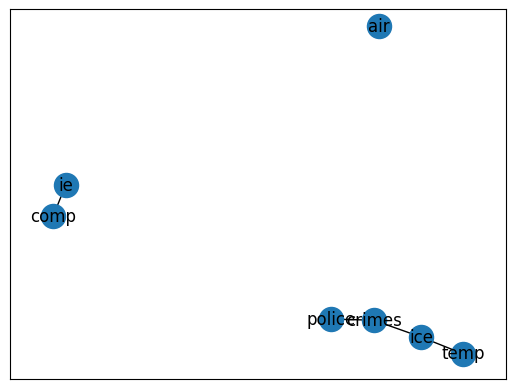
\includegraphics[width=\FigWidth]{figures/practice/chapter-7/sem11-cell43-out0.png}
\caption{Семинар~11: вилка, $Y$ vs $X$. Обратите внимание на сильную связь без учёта $Z$.}
\label{fig:p7-fork1}
\end{figure}
\begin{figure}[htbp]
\centering
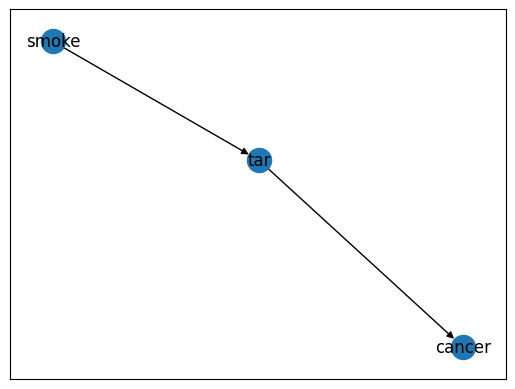
\includegraphics[width=\FigWidth]{figures/practice/chapter-7/sem11-cell51-out0.png}
\caption{Семинар~11: вилка, $Y$ vs $X+Z$. На графике видно ослабление коэффициента при $X$.}
\label{fig:p7-fork2}
\end{figure}
\medskip\noindent\textbf{Три вопроса.} \textit{Постановка:} симуляция DAG-вилки. 
\textit{Применимость:} регрессия не заменяет $do(X)$; блокировать $Z$. 
\textit{Вывод:} маргинальный коэффициент вводит в заблуждение.\medskip

\paragraph{Коллайдер (sem11).}
$X$ и $Y$ независимы, но при отборе $|Z|>c$ появляется ложная корреляция.
\begin{figure}[htbp]
\centering
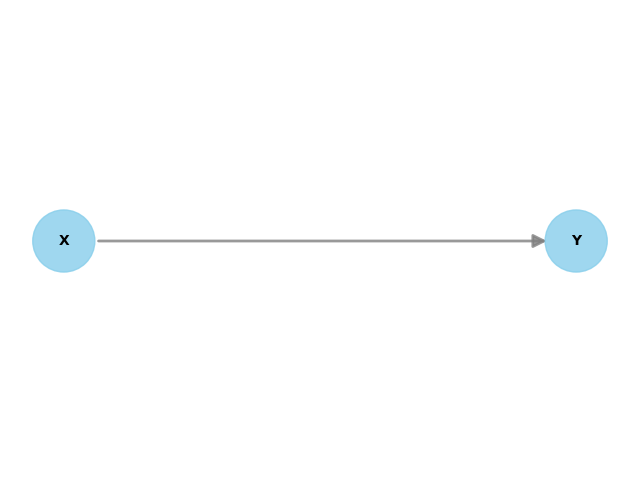
\includegraphics[width=\FigWidth]{figures/practice/chapter-7/sem11-cell61-out2.png}
\caption{Семинар~11: коллайдер. Обратите внимание на корреляцию в подвыборке при $|Z|>c$.}
\label{fig:p7-coll}
\end{figure}
\medskip\noindent\textbf{Три вопроса.} \textit{Постановка:} $X\perp Y$, отбор по коллайдеру $Z$. 
\textit{Применимость:} не включать $Z$ в критерий задней двери (KЗД); объяснять selection bias. 
\textit{Вывод:} условная зависимость --- артефакт отбора.\medskip

\paragraph{Brown, HMM без учителя (sem12).}
Баум--Уэлх на подкорпусе Brown: лог-правдоподобие растёт до плато. Матрица $A$ (рис.~\ref{fig:p7-hmm-trans}).
\begin{figure}[htbp]
\centering
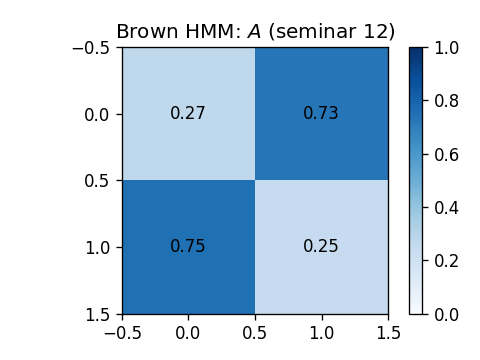
\includegraphics[width=\FigWidth]{figures/practice/chapter-7/sem12-brown-trans-unsupervised.png}
\caption{Семинар~12: матрица $A$ (unsupervised). На графике видно различие диагоналей.}
\label{fig:p7-hmm-trans}
\end{figure}
\medskip\noindent\textbf{Три вопроса.} \textit{Постановка:} символы Brown, скрытые состояния. 
\textit{Применимость:} EM до плато; смотреть $A$, не только LL. 
\textit{Вывод:} метки состояний произвольны, сравнивать с supervised.\medskip

\paragraph{Brown, HMM с разметкой.}
$A$, $B$ по частотам на размеченном корпусе; сравнение с unsupervised --- иная интерпретация состояний, тот же Витерби.
\medskip\noindent\textbf{Три вопроса.} \textit{Постановка:} размеченный vs скрытый HMM. 
\textit{Применимость:} supervised --- частоты; unsupervised --- EM. 
\textit{Вывод:} декодирование одно, интерпретация состояний разная.\medskip

\paragraph{Языковая модель (корпус Jack).}
$n$-граммы, $\chi^2$, перплексия, сглаживание Лапласа; частоты (рис.~\ref{fig:p7-jack-freq}).
\begin{figure}[htbp]
\centering
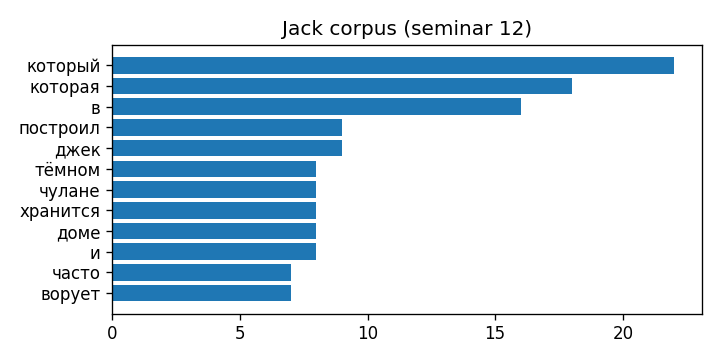
\includegraphics[width=\FigWidth]{figures/practice/chapter-7/sem12-jack-wordfreq.png}
\caption{Семинар~12: частоты слов Jack. Обратите внимание на служебный каркас текста.}
\label{fig:p7-jack-freq}
\end{figure}
\medskip\noindent\textbf{Три вопроса.} \textit{Постановка:} корпус Jack, $n$-граммы. 
\textit{Применимость:} $\chi^2$ на биграммы, перплексия, сглаживание Лапласа. 
\textit{Вывод:} низкая перплексия на повторяющемся тексте не заменяет отложенную выборку (holdout).\medskip

\paragraph{Домашнее sem12.}
Бинарная последовательность по почте: оценить $A$ и сравнить с семинаром.
\medskip\noindent\textbf{Три вопроса.} \textit{Постановка:} своя бинарная цепь. 
\textit{Применимость:} оценка $A$ для двух состояний. 
\textit{Вывод:} сверка с семинарской $A$, не только LL.\medskip

По итогам: DAG и регрессия; HMM --- EM, $A$, $B$; LM --- перплексия и сглаживание.

\section{Контрольные вопросы по теме}

\begin{enumerate}
    \item Объясните парадокс Симпсона на примере лекарства и пола.
    \item Почему в примере~2 (давление) KЗД по $Z$ неверен?
    \item Приведите пример вилки и объясните, почему $Y\perp Z\mid X$.
    \item Запишите формулу задней двери и роль балла включения.
    \item Как PC-алгоритм ориентирует v-структуру $A\to C\leftarrow B$?
    \item Сформулируйте $H_0$ в тесте Грейнджера и статистику $F$.
    \item Вычислите $\mathbb{E}T_i$ для $P_{ii}=0{,}8$.
    \item Для «Дом, который построил Джек» почему перплексия низкая
          без отложенной выборки?
    \item Запишите рекурсию прямого хода и отличие Витерби от $\gamma_t(i)$.
    \item Как устроен M-шаг Баума--Уэлча для $a_{ij}$?
    \item Опишите HMM для разметки частей речи. Что в $A$, что в $B$?
    \item Почему коллайдер нельзя включать в KЗД-множество?
    \item Почему $\sum_j a_{ij}=1$ для каждой строки $i$?
    \item Как изменится $A$ при увеличении \texttt{max\_iterations}?
    \item Сравните лог-правдоподобие на обучении и на отложенной выборке отрезка. Нужна ли большая $n$?
\end{enumerate}

\chapter{Байесовский вывод, априорные распределения и выбор моделей}
\label{ch:bayes}

Частотный подход трактует параметр $\theta$ как фиксированную константу, а случайность~--- в данных.
Байесовский подход объявляет $\theta$ случайной величиной с априорным распределением $p(\theta)$, обновляемым по наблюдениям до апостериорного $p(\theta\mid X)$ \citep{gelman2013,wasserman2004}.
Это даёт полное распределение неопределённости, достоверные интервалы, апостериорное прогнозное распределение для новых наблюдений и естественный механизм выбора моделей через маргинальное правдоподобие.

В гл.~\ref{ch:hypothesis} мы трактовали p-value и доверительные интервалы как свойства процедуры при фиксированном $\theta$. В гл.~\ref{ch:regression} гребневая и lasso-регуляризация уже выступали как штрафы к правдоподобию.
Байесовский вывод делает эту связь явной. Априор $p(\theta)$ и правдоподобие $p(X\mid\theta)$ объединяются в одну плотность, а неопределённость после данных выражается распределением, а не единственной точкой (МП или МНК).
Для последовательных моделей (гл.~\ref{ch:causality}, HMM) EM и Баума--Уэлча~--- частотные аналоги итеративного уточнения. MCMC и VI дают байесовскую альтернативу, когда апостериор не вычисляется аналитически.

\section{Формула Байеса и вывод}

Для параметра $\theta$ и данных $X=(X_1,\ldots,X_n)$: \[ p(\theta\mid X)=\frac{p(X\mid\theta)\,p(\theta)}{p(X)}, \qquad p(X)=\int p(X\mid\theta)\,p(\theta)\,\mathrm{d}\theta.
\] Формула Байеса~--- тот же закон условной вероятности, что лежит в основе цепи Маркова и HMM (гл.~\ref{ch:causality}). Апостериор пропорционален произведению правдоподобия на априор при фиксированных данных.
Логарифм апостериорной плотности: \[ \log p(\theta\mid X)=\log p(X\mid\theta)+\log p(\theta)+\mathrm{const}.
\] Нормировочная константа $p(X)$~--- маргинальное правдоподобие. Она не нужна для MAP и MCMC, но критична при сравнении моделей.

\begin{definition}
MAP-оценка $\hat\theta_{\mathrm{MAP}}=\arg\max_\theta p(\theta\mid X)$ совпадает с регуляризованным МП. Априорное $\log p(\theta)$ играет роль штрафа (аналогично ridge/lasso в гл.~\ref{ch:regression}).
\end{definition}

\begin{definition}
Семейство априоров сопряжено правдоподобию, если апостериор принадлежит тому же семейству, что и априор.
\end{definition}

\section{Пример: монетка и бета-априор}

В примере с монетой зафиксированы десять подбрасываний. Семь орлов и три решки. Модель: $X_i\mid p\sim \mathrm{Bern}(p)$ i.i.d.
Это та же схема успех/неуспех, что в биномиальных тестах (гл.~\ref{ch:hypothesis}), но параметр $p$ трактуется как случайная величина, а не как фиксированная частота генерации.

Априор $p\sim \mathrm{Beta}(\alpha,\beta)$.
Правдоподобие $p(X\mid p)=p^{\sum X_i}(1-p)^{n-\sum X_i}$.
Апостериор.\[ p\mid X \sim \mathrm{Beta}\!\left(\alpha+\sum X_i,\;\beta+n-\sum X_i\right).
\] MAP (при $\alpha,\beta>1$): $\hat p=\frac{\alpha+\sum X_i-1}{\alpha+\beta+n-2}$.
Апостериорное среднее $\mathbb{E}(p\mid X)=\frac{\alpha+\sum X_i}{\alpha+\beta+n}$.
При $\mathrm{Beta}(1,1)$ и $k=7$ орлов: $p\mid X\sim\mathrm{Beta}(8,4)$, $\mathbb{E}(p\mid X)=0{,}667$.
На рис.~\ref{fig:beta-posterior}~--- апостериорная плотность при симметричном априоре $\mathrm{Beta}(1,1)$ и данных 7H/3T.

\begin{figure}[htbp]
    \centering
    
\includegraphics[width=\FigWidth]{\FigDir/chapter-8/beta.png}
    \caption{Апостериорное распределение $p$ (Beta).}
    \label{fig:beta-posterior}
\end{figure}

При пяти орлах подряд МП даёт $\hat p=0$ для вероятности решки. Байесовский вывод с умеренным априором (например, $\mathrm{Beta}(2,2)$) сохраняет ненулевую вероятность хвоста~--- это иллюстрация роли априора при малых $n$.
Достоверный интервал для $p$ при $\mathrm{Beta}(8,4)$ интерпретируется как вероятность параметра в интервале равна 95\% после наблюдения данных~--- в отличие от частотного ДИ (гл.~\ref{ch:basics},~\ref{ch:hypothesis}).
При 7H/3T и $\mathrm{Beta}(1,1)$ апостериор $\mathrm{Beta}(8,4)$. Апостериорное среднее $2/3$, HPD смещён относительно интервала с равными хвостами. Прогнозное $P(\text{next H})=8/12$.
Та же цепочка априор $\to$ данные $\to$ апостериор $\to$ прогноз повторяется в NIG и Gamma--Poisson.

\section{Сопряжённые семейства}

Нормальная модель: Normal--Inverse-Gamma. Данные $X_i\mid\mu,\sigma^2\sim\mathcal{N}(\mu,\sigma^2)$ i.i.d.
Сопряжённый априор на $(\mu,\sigma^2)$: \[ \mu\mid\sigma^2 \sim \mathcal{N}(\mu_0,\,\sigma^2/\kappa_0), \qquad \sigma^2 \sim \mathrm{Inv\text{-}Gamma}(\alpha_0,\,\beta_0).
\] Апостериор после $n$ наблюдений с $\bar x$, $s^2$: \[ \mu\mid\sigma^2,X \sim \mathcal{N}\!\left(\mu_n,\,\frac{\sigma^2}{\kappa_n}\right), \quad \sigma^2\mid X \sim \mathrm{Inv\text{-}Gamma}(\alpha_n,\beta_n), \] где $\kappa_n=\kappa_0+n$, $\mu_n=\frac{\kappa_0\mu_0+n\bar x}{\kappa_n}$, $\alpha_n=\alpha_0+n/2$, $\beta_n=\beta_0+\frac12\sum(x_i-\bar x)^2+\frac{\kappa_0 n(\bar x-\mu_0)^2}{2\kappa_n}$.
Маргинальный апостериор $\mu\mid X$~--- распределение Стьюдента. Достоверный интервал для $\mu$ не совпадает с частотным $t$-интервалом при том же $\alpha$, хотя при больших $n$ близок.
NIG-модель~--- байесовский аналог линейной регрессии с неизвестной дисперсией. Априор на $(\mu,\sigma^2)$ заменяет фиксированное $\sigma^2$ в классическом МНК и даёт $t$-подобные хвосты для $\mu\mid X$.

Пуассон и гамма. Счётчики $N_i\mid\lambda\sim\mathrm{Poisson}(\lambda)$: \[ p(N\mid\lambda)\propto \lambda^{\sum N_i} e^{-\lambda n}.
\] Сопряжённый априор: $\lambda\sim\mathrm{Gamma}(\alpha,\beta)$ (параметризация $\mathrm{rate}=\beta$): \[ \lambda\mid N \sim \mathrm{Gamma}\!\left(\alpha+\sum N_i,\;\beta+n\right).
\] Апостериорное среднее: $\mathbb{E}(\lambda\mid N)=\frac{\alpha+\sum N_i}{\beta+n}$.

Апостериорное прогнозное распределение (прогноз нового наблюдения) интегрирует правдоподобие по апостериору \[ p(X_{\mathrm{new}}\mid X)=\int p(X_{\mathrm{new}}\mid\theta)\,p(\theta\mid X)\,\mathrm{d}\theta.
\] Прогнозное распределение шире, чем подстановка $\hat\theta$. Оно учитывает неопределённость параметра~--- аналог доверительного прогнозного интервала в регрессии, но в чисто байесовской форме.
Beta--Binomial: при $p\mid X\sim\mathrm{Beta}(a,b)$ \[ P(X_{\mathrm{new}}=1\mid X)=\frac{a}{a+b}.
\] Нормальное--Стьюдента: при NIG-апостериоре предсказание для одного $X_{\mathrm{new}}$~--- $t$-распределение с тяжёлыми хвостами (учёт неопределённости $\sigma^2$).
Gamma--Poisson: предсказание~--- отрицательное биномиальное распределение для счётчиков.
Сопряжённость удобна аналитически, но не обязательна. Для произвольного априора используют MCMC, вариационный вывод (VI) или сеточные аппроксимации.
При большом $n$ апостериор определяется правдоподобием. Слабый априор подавляется данными. VI минимизирует $KL(q(\theta)\|p(\theta\mid X))$ внутри семейства $q$ (например, факторизованное гауссово). Быстрее MCMC, но смещение при узком $q$.
Для Beta--Binomial новый орёл учитывает неопределённость $p$, а не только $\bar x$.
В гл.~\ref{ch:basics} частотный интервал для $p$ описывает процедуру при фиксированном $p$. Прогнозное $P(X_{\mathrm{new}}=1\mid X)$~--- распределение будущего наблюдения при текущих данных.

\begin{center}
\footnotesize
\begin{tabular}{lllll}
\toprule
Правдоподобие & Параметр & Априор & Апостериор (параметры) \\
\midrule
Бернулли / биномиальное & $p$ & $\mathrm{Beta}(\alpha,\beta)$ &
$\mathrm{Beta}(\alpha{+}k,\,\beta{+}n{-}k)$, $k=\sum x_i$ \\
Нормальное, $\sigma^2$ известна & $\mu$ & $\mathcal{N}(\mu_0,\sigma_0^2)$ &
$\mathcal{N}(\mu_n,\sigma_n^2)$, $\mu_n=\frac{\sigma_0^{-2}\mu_0+n\sigma^{-2}\bar x}{\sigma_0^{-2}+n\sigma^{-2}}$ \\
Нормальное, $\mu$ известно & $\sigma^2$ & $\mathrm{Inv\text{-}}\Gamma(\alpha_0,\beta_0)$ &
$\mathrm{Inv\text{-}}\Gamma(\alpha_n,\beta_n)$ \\
Нормальное i.i.d. & $(\mu,\sigma^2)$ & NIG &
$\mu\mid\sigma^2,X\sim\mathcal{N}(\mu_n,\sigma^2/\kappa_n)$,
$\sigma^2\mid X\sim\mathrm{Inv\text{-}}\Gamma(\alpha_n,\beta_n)$ \\
Пуассон & $\lambda$ & $\mathrm{Gamma}(\alpha,\beta)$ (rate) &
$\mathrm{Gamma}(\alpha{+}{\sum N_i},\,\beta{+}n)$ \\
Мультиномиальное & $\mathbf{p}$ & $\mathrm{Dir}(\boldsymbol{\alpha})$ &
$\mathrm{Dir}(\boldsymbol{\alpha}+\mathbf{n})$ \\
\bottomrule
\end{tabular}
\end{center}

\section{Назначение априорных распределений}

Информативный априор отражает экспертные знания или прошлые эксперименты (например, $\mathrm{Beta}(2,2)$~--- умеренное смещение к $p=0{,}5$).
Неинформативный / слабоинформативный.~--- широкая поддержка ($\mathrm{Beta}(1,1)$, нормальный с большой дисперсией, равномерный на $[-50,50]$ для температуры).
Выбор между ними~--- вопрос контекста. В промышленном контроле качества разумен информативный априор от прошлых партий. В разведочном анализе~--- слабый, чтобы данные доминировали.
Распределение Джеффриса: $p(\theta)\propto\sqrt{\det I(\theta)}$, инвариантно к репараметризации. Для Бернулли $p(p)\propto p^{-1/2}(1-p)^{-1/2}$ (Beta$(\tfrac12,\tfrac12)$). Для среднего нормального~--- $p(\mu)\propto 1$. Для $\sigma$~--- $p(\sigma)\propto 1/\sigma$.
\begin{itemize}
    \item Априор, противоречащий механизму генерации данных, смещает вывод
          даже при больших $n$ (несобственные априоры требуют проверки нормируемости апостериора).
    \item Достоверный и доверительный интервалы по формулировке
          часто путают. 95\% ДИ~--- свойство процедуры. 95\% достоверный~--- вероятность параметра после наблюдения данных.
    \item Несобственный равномерный на $\mathbb{R}$ для дисперсии не даёт нормируемого
          апостериора в малых выборках.
\end{itemize}

Выбор априора~--- часть постановки. $\mathrm{Beta}(2,2)$ кодирует умеренное предположение о справедливости монетки до данных. $\mathrm{Beta}(1,1)$~--- максимальную неопределённость. Анализ чувствительности повторяет вывод при трёх априорах. Если MAP и HPD радикально различаются при $n=20$, данные ещё не доминируют~--- это нормально сообщать в отчёте, а не подбирать априор.

\section{Связь с регуляризацией}

Для нормального правдоподобия с гауссовым априором на коэффициенты: \[ \log p(\beta\mid X,y)\propto -\frac1{2\sigma^2}\|y-X\beta\|_2^2-\frac1{2\tau^2}\|\beta\|_2^2 \] ~--- ridge ($l_2$). Априор Лапласа $\Rightarrow$ lasso ($l_1$).
Регуляризация Фирта в логистической регрессии~--- байесовский штраф Джеффриса-подобного вида при разделимости классов (линейно разделимые классы).
Интерпретация. $\tau^2$ в ridge~--- дисперсия априора на $\beta$. Чем меньше $\tau$, тем сильнее сжатие коэффициентов к нулю.
Lasso соответствует априору Лапласа с экспоненциальными хвостами, что объясняет разреженность MAP-оценок.
В гл.~\ref{ch:regression} ridge MAP $\Leftrightarrow$ $l_2$-штраф, lasso MAP $\Leftrightarrow$ $l_1$. Байесовский вывод делает штраф
интерпретируемым как $\log p(\beta)$. При мультиколлинеарности гауссов априор стабилизирует $\hat\beta_{\mathrm{MAP}}$ так же, как ridge стабилизирует МНК~--- различие в интерпретации (распределение и частотная процедура), сходство в формуле.

\section{Достоверные интервалы}

\begin{definition}
$(1-\alpha)$-достоверный интервал $[a,b]$ удовлетворяет $P(\theta\in[a,b]\mid X)=1-\alpha$.
\end{definition}

С равными хвостами: квантили $\alpha/2$ и $1-\alpha/2$ апостериора.
HPD (наибольшая апостериорная плотность) даёт кратчайший интервал с массой $1-\alpha$.
Для $\mathrm{Beta}(8,4)$ HPD смещён относительно интервала с равными хвостами при асимметрии. При $\alpha+\beta+n$ большом различие мало.
В отчёте по практической задаче (гл.~\ref{ch:labs}) для вероятностных моделей предпочтительно указывать и точечную оценку (среднее/MAP), и HPD~--- особенно при асимметричном апостериоре и малых $n$.
Чувствительность к априору. При $n=10$, $\bar X=0{,}17$, $X_i\sim\mathcal{N}(0,1)$ частотный 95\% ДИ для $\mu$~--- $[-0{,}45,\,0{,}78]$, а при сильном априоре $\mu\sim\mathcal{N}(0,0{,}01)$ достоверный~--- $[-0{,}002,\,0{,}03]$. При $n=10^5$ оба сужаются к $[0{,}164,\,0{,}176]$, но априор всё ещё слегка смещает центр.
Анализ чувствительности повторяет вывод при нескольких разумных априорах (информативный, слабый, Джеффриса) и сравнивает MAP, достоверный интервал и апостериорное прогнозное распределение. Существенный разброс при фиксированном $n$~--- сигнал, что данные не доминируют над априором.
Практически достоверный интервал строят из сэмплов MCMC или аналитически для сопряжённых семейств. С равными хвостами проще, HPD короче при асимметрии. В отчёте указывают тип интервала. 95\% достоверный с равными хвостами и 95\% HPD могут слегка отличаться при $\mathrm{Beta}(8,4)$.

\section{Аппроксимативный вывод: MCMC}

Когда $p(\theta\mid X)$ не вычисляется в замкнутой форме, сэмплируют из апостериора.

Metropolis--Hastings:.\begin{enumerate}
    \item Предложение $z'\sim q(z'\mid z^{(t)})$.
    \item Принять с вероятностью
          $A=\min\!\left(1,\dfrac{p(z')\,q(z^{(t)}\mid z')}{p(z^{(t)})\,q(z'\mid z^{(t)})}\right)$.
    \item Если принято, $z^{(t+1)}=z'$; иначе $z^{(t+1)}=z^{(t)}$.
\end{enumerate}
Достаточно знать $p$ с точностью до нормировки. Цепь имеет стационарное распределение $p(z\mid X)$ при симметричном $q$ (случайного блуждания Метрополиса).
MCMC~--- частотный способ получить байесовские интегралы. Среднее по сэмплам аппроксимирует $\mathbb{E}(\theta\mid X)$, квантили~--- достоверные интервалы.
Сэмплы коррелированы. Для оценок берут выход на стационарность и прореживание (каждый $k$-й сэмпл). Диагностика включает графики траекторий. $\hat R>1$ указывает на плохую сходимость цепей.
Доля принятия и длина выхода на стационарность зависят от формы апостериора. Типичная последовательность шагов. Задать априор и правдоподобие $\to$ запустить цепь $\to$ проверить траекторию и $\hat R$ $\to$ построить достоверный интервал и прогнозное распределение $\to$ при необходимости сравнить модели через BF или BIC.
Без диагностики сходимости байесовский интервал~--- иллюзия точности.

\section{Выбор моделей}

Пусть $\mathcal{M}_k$~--- модель с параметром $\theta_k$.
Фактор Байеса:.\[ BF_{10}=\frac{p(X\mid\mathcal{M}_1)}{p(X\mid\mathcal{M}_0)}= \frac{\int p(X\mid\theta_1,\mathcal{M}_1)p(\theta_1\mid\mathcal{M}_1)\,\mathrm{d}\theta_1} {\int p(X\mid\theta_0,\mathcal{M}_0)p(\theta_0\mid\mathcal{M}_0)\,\mathrm{d}\theta_0}.
          \]

\begin{center}
\small
\begin{tabular}{cl}
\toprule
$BF_{10}$ & Сила доказательств (Джеффриса) \\
\midrule
$<1$ & доказательства в пользу $\mathcal{M}_0$ \\
$1$--$3$ & слабые \\
$3$--$10$ & умеренные \\
$10$--$30$ & сильные \\
$30$--$100$ & очень сильные \\
$>100$ & решительные \\
\bottomrule
\end{tabular}
\end{center}

Evidence $p(X\mid\mathcal{M})=\int p(X\mid\theta)p(\theta\mid\mathcal{M})\,\mathrm{d}\theta$ штрафует сложные модели (Occam factor).
Интуиция. Модель с большим числом параметров может подогнать данные лучше, но размазанный по $\theta$ априор снижает среднее правдоподобие после интегрирования~--- тот же дух, что штраф $k$ или $k\ln n$ в AIC/BIC (гл.~\ref{ch:regression}).
AIC $=-2\log L+2k$~--- асимптотическая аппроксимация для слабых априоров. BIC $=-2\log L+k\ln n$~--- ближе к фактор Байеса при априор с единичной информацией.
MDL: $\mathrm{MDL}(\mathbf{f},\mathfrak{D})=L(\mathbf{f})+L(\mathfrak{D}\mid\mathbf{f})$. При больших $n$ связан с BIC.
Savage--Dickey (вложенные модели). Если $\mathcal{M}_0$ получается из $\mathcal{M}_1$ при $\theta=\theta_0$, то \[ BF_{10}=\frac{p(\theta_0\mid\mathcal{M}_1,X)}{p(\theta_0\mid\mathcal{M}_1)}.
\] Нужна только апостериорная плотность под $\mathcal{M}_1$ в точке $\theta_0$ и априор~--- удобно для сравнения эффекта / отсутствия эффекта в регрессии (гл.~\ref{ch:regression}). $\mathcal{M}_0$~--- модель без предиктора, $\mathcal{M}_1$~--- с ним. $\theta_0=0$ для коэффициента.
Аппроксимация Лапласа: $\log p(X\mid\mathcal{M})\approx \log p(X\mid\hat\theta)\,p(\hat\theta\mid\mathcal{M}) -\frac{k}{2}\log(2\pi)+\frac12\log\det H^{-1}$, где $H$~--- гессиан $-\log p(\theta\mid X)$ в моде.
Для $g$-априор на $\beta$ в линейной регрессии маргинальное правдоподобие выписывается аналитически.
Вычисление маргинального правдоподобия многомерно. Оценка гармонического среднего MCMC может иметь бесконечную дисперсию. Для вложенных моделей предпочтительны Savage--Dickey или мостовая выборка. BF чувствителен к априору на общих параметрах вложенных моделей (парадокс Линдли при неинформативном априоре на $\theta$).
Линейная регрессия с $g$-априор даёт $p(X\mid\mathcal{M})$ аналитически. Нелинейные модели~--- аппроксимация Лапласа в моде $\hat\theta$ с гессианом $H$. Для не вложенных моделей~--- мостовая выборка или BIC при описании в отчёте. Гармоническое среднее из MCMC для маргинального правдоподобия ненадёжно.
Пример выбора модели в регрессии. $\mathcal{M}_0$ без $x_j$, $\mathcal{M}_1$ с $x_j$. Savage--Dickey даёт $BF_{10}$ через апостериор $\hat\beta_j$ при $\mathcal{M}_1$ в точке 0. Согласование с частичным $F$ из гл.~\ref{ch:regression} при слабом априоре и большом $n$. Расхождение при информативном априоре~--- повод для анализа чувствительности.

\section{Evidence и принцип MDL}

\begin{center}
\small
\begin{tabular}{p{0.42\linewidth}|p{0.42\linewidth}}
\toprule
Evidence $p(X\mid\mathcal{M})=\int p(X\mid\theta)\,p(\theta\mid\mathcal{M})\,\mathrm{d}\theta$
& MDL $\mathrm{MDL}(\mathbf{f},\mathfrak{D})=L(\mathbf{f})+L(\mathfrak{D}\mid\mathbf{f})$ \\
\midrule
Использует априорные знания через $p(\theta\mid\mathcal{M})$
& Минимизирует длину описания данных в битах. Априор не обязателен \\
\midrule
Опирается на вероятностную модель порождения выборки
& Сравнивает модели по коду без явной генеративной модели \\
\midrule
фактор Байеса, Savage--Dickey, Laplace
& Связь с BIC при больших $n$: $\mathrm{BIC}\approx -2L+\log n\,(k{+}1)$ \\
\bottomrule
\end{tabular}
\end{center}

При большом $n$ MDL разлагается на три слагаемых (длины в битах): \[ \mathrm{MDL}(\mathbf{f},\mathfrak{D}) \approx \underbrace{L(\mathbf{f})}_{\text{сложность модели}} + \underbrace{L(\mathbf{w}^*\mid\mathbf{f})}_{\text{код параметров}} + \underbrace{L(\mathfrak{D}\mid\mathbf{w}^*,\mathbf{f})}_{\text{остаток / шум}}, \] где $\mathbf{w}^*$~--- МП- или MAP-параметры при фиксированной структуре $\mathbf{f}$.
Первое слагаемое штрафует богатые модели (Occam). Третье~--- fit данных.
Evidence $p(X\mid\mathcal{M})$ интегрирует по $\theta$ и даёт тот же дух штрафа за сложность (Occam factor), но явно через априор.

Колмогоровская сложность (длина минимального программы для $\mathfrak{D}$) невычислима. MDL~--- вычислимый практический принцип. Теорема инвариантности даёт близость кодов на разных языках только асимптотически при больших $n$.

\section{Схема байесовского анализа}

\begin{enumerate}
    \item Задать правдоподобие $p(X\mid\theta)$ и осмысленный априор $p(\theta)$.
    \item Аналитический апостериор, сетку, вариационный вывод или MCMC (MH, HMC).
    \item Проверить сходимость ($\hat R$, графики траекторий).
    \item Сообщить среднее/медиана, 95\% достоверный, HPD. Апостериорное прогнозное распределение
          для прогноза.
    \item При нескольких $\mathcal{M}_k$~--- фактор Байеса (Savage--Dickey,
          Laplace, BIC) и анализ чувствительности по априору.
\end{enumerate}
Схема повторяет логику практических задач (гл.~\ref{ch:labs}). Сначала явная модель и предпосылки, затем оценивание, диагностика и интерпретация с учётом альтернативных априоров.
Для HMM (гл.~\ref{ch:causality}) EM даёт MAP-подобную точку. Полный байесовский HMM потребовал бы MCMC по $(A,B,\pi)$~--- тема за рамками курса, но концептуально та же.
В отчёте указывают априор (семейство и параметры), правдоподобие, апостериорное распределение (аналитическое/MCMC), точечную оценку (среднее/MAP), 95\% HPD, апостериорное прогнозное распределение при необходимости. Чувствительность~--- 2--3 априора. BF или BIC между моделями. Не используют байесовское p-value~--- вместо этого хвост апостериорного распределения или BF. При MCMC указывают число сэмплов, выход на стационарность и $\hat R$.

\begin{codefragment}
# Beta-Binomial posterior (7 heads, 3 tails)
import numpy as np
from scipy import stats
flips = ["H"] * 7 + ["T"] * 3
n_heads = sum(1 for x in flips if x == "H")
a0, b0 = 1, 1  # uniform prior
a_post = a0 + n_heads
b_post = b0 + len(flips) - n_heads
ci = stats.beta.ppf([0.025, 0.975], a_post, b_post)
pred = a_post / (a_post + b_post)  # P(next H | data)
\end{codefragment}

Пример: монетка, регрессия, выбор модели (1)~7H/3T, $\mathrm{Beta}(1,1)$ априор. Апостериорное распределение $\mathrm{Beta}(8,4)$. 95\% HPD для $p$ не совпадает с частотным интервалом Уилсона~--- разная интерпретация (гл.~\ref{ch:basics}).
(2)~Линейная регрессия с $g$-априор на $\beta$. MAP$=$ridge. При $H_0\colon\beta_j=0$ Savage--Dickey даёт $BF_{10}$ без интеграла по всему пространству.
(3)~Сравнение моделей с 5 и 12 предикторами. BIC и Laplace-аппроксимация маргинального правдоподобия штрафуют сложность. Лучший $R^2$ на обучении может проигрывать по маргинальному правдоподобию на тесте.

Анализ чувствительности по априору. $\mathrm{Beta}(1,1)$ и $\mathrm{Beta}(2,2)$ при $n=10$ заметно сдвигает HPD. При $n=200$ апостериоры почти совпадают~--- данные подавляют слабый априор. MCMC для логистической регрессии со слабо информативным априором на $\beta$ даёт достоверные интервалы для OR, сопоставимые с Уолда, но устойчивее при разделимости классов.

На практике команды смешивают подходы. MLE/МНК для точечной оценки, бутстреп-ДИ для частотной неопределённости, слабый априор для регуляризации, BIC для выбора модели~--- всё это байесовски мотивировано, но не полный апостериорный отчёт. Полный байесовский отчёт добавляет явный априор, апостериорное распределение (аналитическое или MCMC), HPD, апостериорное прогнозное распределение и BF между моделями. Важно понимать, какой уровень байесовскости использован. Путаница между достоверным интервалом и доверительным~--- частая ошибка (см. гл.~\ref{ch:basics}).
При $n\gg 1$ априор подавляются данными, и подходы сходятся. При малых $n$ различие принципиально.
Слабые априоры и большие $n$ дают апостериор, близкий к правдоподобию, и достоверный интервал $\approx$ доверительный. Малые $n$, иерархические модели, явный учёт неопределённости параметра, сравнение моделей через маргинальное правдоподобие, регуляризация с интерпретацией априора~--- сильные мотивации. Несобственные априоры и MCMC без диагностики~--- зона повышенного риска.
Байесовский вывод~--- не отдельная статистика, а явное объединение правдоподобия, априора и прогнозного распределения. Связь с ridge, AIC/BIC и EM (гл.~\ref{ch:causality}) замыкает курс. В отчёте всегда указывают тип интервала (достоверный или доверительный) и проверку чувствительности к априору при малых $n$.

\section{Практика и семинар}
\label{sec:practice-ch8}

Семинар~13 проходит полный байесовский цикл на синтетических монетках с конвейера с визуализацией сопряжённого обновления.

Синтетические монетки. Постановка. Монетки с конвейера. Доля честных с $p=0{,}5$ и смещённых.
Для одной монетки: $X_i\mid p\sim\mathrm{Bern}(p)$ i.i.d., априор $p\sim\mathrm{Beta}(\alpha,\beta)$.

Шаги вычисления:.\begin{enumerate}
    \item Априор. Задайте $(\alpha,\beta)$. $\mathrm{Beta}(1,1)$ --- неинформативный.
          $\mathrm{Beta}(2,2)$ --- умеренное смещение к $0{,}5$.
    \item Данные. $n$ подбрасываний, $k$ орлов. Правдоподобие
          $p(X\mid p)\propto p^k(1-p)^{n-k}$.
    \item Апостериор.
          $p\mid X\sim\mathrm{Beta}(\alpha+k,\,\beta+n-k)$.
    \item Сводки: $\mathbb{E}(p\mid X)=\dfrac{\alpha+k}{\alpha+\beta+n}$.
          MAP при $\alpha,\beta>1$: $\hat p_{\mathrm{MAP}}=\dfrac{\alpha+k-1}{\alpha+\beta+n-2}$.
    \item Интервалы: 95\% достоверный интервал с равными хвостами из квантилей Beta.
          HPD короче при асимметрии (особенно при малых $n$).
    \item Апостериорное прогнозное распределение:
          $P(X_{\mathrm{new}}=1\mid X)=\dfrac{\alpha+k}{\alpha+\beta+n}$.
    \item Анализ чувствительности: повторите шаги 3--6 для трёх априоров. Сравните HPD и MAP.
\end{enumerate}

Анимация обновления (sem13). При последовательном поступлении орлов плотность $\mathrm{Beta}(\alpha+k,\beta+n-k)$ сдвигается вправо. При $P=0{,}5$ генератора и $\mathrm{Beta}(2,2)$ апостериор сходится к $0{,}5$ при $n\to\infty$.

\begin{codefragment}
# Posterior Beta-Binomial (sem13)
import numpy as np
from scipy import stats
k, n = 7, 10          # observed heads and n
a0, b0 = 1, 1         # Beta(1,1) prior
a_post, b_post = a0 + k, b0 + n - k
mean_p = a_post / (a_post + b_post)
hpd = stats.beta.interval(0.95, a_post, b_post)
pred_next = mean_p      # P(next head | data)
\end{codefragment}

Нормальная модель (дополнение sem13). При известной $\sigma^2$ сопряжённый априор $\mu\sim\mathcal{N}(\mu_0,\sigma_0^2)$ даёт $\mu\mid X\sim\mathcal{N}(\mu_n,\sigma_n^2)$ с $\mu_n=\bigl(\frac{\mu_0}{\sigma_0^2}+\frac{n\bar x}{\sigma^2}\bigr) \bigl(\frac{1}{\sigma_0^2}+\frac{n}{\sigma^2}\bigr)^{-1}$.
Сравните 95\% достоверный для $\mu$ с частотным $t$-интервалом при том же $\alpha$.

Отчёт: укажите априор, правдоподобие, апостериорное распределение (график), среднее/MAP, 95\% HPD, прогнозное распределение для одного нового наблюдения. Не путайте достоверный интервал с ДИ (гл.~\ref{ch:basics},~\ref{ch:hypothesis}).

\section{Контрольные вопросы по теме}

\begin{enumerate}
    \item Сформулируйте различие между достоверным интервалом и доверительным
          интервалом (см. также гл.~\ref{ch:basics}).
    \item Покажите, что $\mathrm{Beta}(1,1)$ априор для монетки даёт апостериор
          $\mathrm{Beta}(1+k,\,1+n-k)$ при $k$ орлах.
    \item Запишите апостериор NIG для $(\mu,\sigma^2)$ в одной строке
          для $\mu_n$.
    \item Выведите апостериорное прогнозное распределение для Beta--Binomial.
    \item Почему $\log p(\theta\mid X)$ можно трактовать как правдоподобие плюс штраф?
    \item Запишите долю принятия Metropolis--Hastings.
    \item Что такое фактор Байеса и как он связан с маргинальным правдоподобием?
    \item Как применить Savage--Dickey для $H_0\colon\beta=0$ в регрессии?
    \item Интерпретируйте строку $BF_{10}\in(3,10)$ по шкале Джеффриса.
    \item Когда BIC и фактор Байеса дают согласованный выбор модели?
    \item Зачем нужно распределение Джеффриса, если есть равномерный априор?
    \item Как интерпретировать апостериорное среднее $p=0{,}7$ против MAP $p=0{,}68$
          при одном и том же априоре?
    \item Приведите пример, когда сильный априор и малый $n$ радикально
          меняют достоверный интервал.
    \item Чем VI отличается от MCMC по ошибке аппроксимации?
\end{enumerate}

\chapter{Практические задачи}
\label{ch:labs}

Практический блок курса охватывает проверку гипотез, множественные сравнения, регрессию, временные ряды, причинность и марковские модели.
Формулировки задач приведены в настоящей главе.
Численные таблицы и описание переменных --- в приложении~\ref{app:lab-data}.
Тексты, изображения и аудиозаписи, не помещающиеся в приложение, указаны сносками к соответствующим задачам.
Подмножество задач для сдачи назначает преподаватель (вариант выдаётся скриптом в репозитории курса, \PSADRepo{}).

Каждое задание оформляется в электронном рабочем тетради курса: в начале --- номер и формулировка, далее --- графики, расчёты и выводы. Язык вычислений не фиксируется.
Разобранные шаги семинаров (загрузка данных, тесты, модели) --- в \S\S\ref{sec:practice-ch2}--\ref{sec:practice-ch8}; здесь --- только постановки лабораторных работ.

\begin{table}[htbp]
\centering
\caption{Соответствие лабораторных работ, глав и раздела «Практика и семинар»}
\label{tab:lab-theory-practice}
\footnotesize
\begin{tabularx}{\linewidth}{|l|X|X|}
\hline
\textbf{Блок} & \textbf{Главы теории} & \textbf{Разбор в книге} \\
\hline
Лаб.\ 1, зад.\ 1 (GOF, мощность) & \ref{ch:hypothesis}, \S\ref{sec:gof-ch2} & \ref{sec:practice-ch2} \\
Лаб.\ 1, зад.\ 1.2--1.4 & \ref{ch:hypothesis}, \ref{ch:multiple} & \ref{sec:practice-ch2}, \ref{sec:practice-ch3} \\
Лаб.\ 1, зад.\ 2 (регрессия) & \ref{ch:regression} & \ref{sec:practice-ch5} \\
Лаб.\ 2, ряды и SPRT & \ref{ch:timeseries} & \ref{sec:practice-ch6} \\
Лаб.\ 2, DAG и HMM & \ref{ch:causality} & \ref{sec:practice-ch7} \\
Лаб.\ 2, байес (при необходимости) & \ref{ch:bayes} & \ref{sec:practice-ch8} \\
\hline
\end{tabularx}
\end{table}

\section{Лабораторная работа~1}
\label{sec:lab1-tasks}

Первый блок опирается на главы~\ref{ch:hypothesis}--\ref{ch:regression}.
Теоретические задачи требуют полного аналитического вывода: все переходы описаны, выкладки и преобразования явно посчитаны (см.~\S\ref{sec:report-requirements}).

\subsection{Задание 1}


\subsubsection{Задача 1.1}

Проверить мощность и консервативность критериев Лиллиефорса, Харке--Бера, Шапиро--Уилка для выборок из следующих распределений:
\begin{itemize}
    \item Нормальное
    \item Лапласа
    \item Стьюдента
    \item Усеченное нормальное распределение (модуль каждого элемента выборки не превосходит 2)
\end{itemize}

\subsubsection{Задача 1.2}

Задана выборка описаний 150 экземпляров ириса разных видов \citep{fisher1936}. Описание каждого ириса состоит из четырёх признаков:
\begin{itemize}
    \item длина наружной доли околоцветника (sepal length)
    \item ширина наружной доли околоцветника (sepal width)
    \item длина внутренней доли околоцветника (petal length)
    \item ширина внутренней доли околоцветника (petal width)
\end{itemize}
Требуется определить, насколько в среднем различается каждая из этих характеристик между разными видами.
Для каждой характеристики выбрать подходящий размер эффекта \citep{ellis2010} и посчитать соответствующее значение.

\subsubsection{Задача 1.3}

Проверить мощность и консервативность критерия Уилкоксона о равенстве медиан для выборок вида:
X1: ~ $\alpha$ * N(0,1) + (1-$\alpha$) * N(2, 4);

X2: ~ $\alpha$ * N(0,1) + (1-$\alpha$) * N(2, 4) + $\delta$.

Здесь $\delta$ --- сдвиг, дающий возможность разделить выборки X1 и X2.
Изучить зависимость от $\alpha$ и $\delta$.
Распределение является гауссовой смесью, а не суммой независимых гауссовых величин. Для генерации выборки достаточно на каждом шаге выбирать компоненту смеси с вероятностями $(\alpha, 1-\alpha)$ и сэмплировать из соответствующего нормального закона.

\subsubsection{Задача 1.4}

Частота слов в тексте часто описывается законом Ципфа \citep{zipf1949}. В выборке из $N$ различных слов вероятность слова ранга $k$ аппроксимируется $P(k) \propto k^{-a}$, где $a>0$ --- параметр распределения.
Проверить формальным критерием, насколько закон Ципфа описывает частоты слов в двух корпусах: романе «Анна Каренина» и новостном корпусе OPUS-WMT-News.\footnote{Тексты корпусов: \url{http://az.lib.ru/t/tolstoj_lew_nikolaewich/text_0080.shtml} и \url{https://object.pouta.csc.fi/OPUS-WMT-News/v2019/mono/ru.txt.gz}.}
Можно ли утверждать, что параметры $a$ для этих двух корпусов совпадают?

\subsection{Задание 2}


\subsubsection{Задача 2.1}

Пусть задано два вектора ответов: $y$ --- истинный вектор ответов для некоторой выборки, а также есть вектор ответов $\hat{y}$ --- некоторой предсказательной модели. Наблюдатель хочет проверить гипотезу о том, что ровно в 25\% случаев модель даёт заниженные оценки.
Предложите метод проверки данной гипотезы: запишите задачу формально,
предложите статистику для решения данной задачи на уровне значимости $\alpha=0{,}05$.
Также найдите зависимость мощности данного критерия в зависимости от истинного процента заниженных ответов.
Все выкладки должны быть сделаны аналитически, без использования компьютера (допускается использование компьютера для подстановки численных значений в финальную формулу).

\subsubsection{Задача 2.2}

Рассмотрим фирму, которая занимается продажей лотерейных билетов. Правила лотереи следующие: все билеты являются выигрышными с вероятностью $p$. Билеты продаются до тех пор, пока хоть один человек не выиграет (гарантируется, что как только билет купили и он выигрышный, больше билетов не продают).
Из-за вспышки коронавируса все заводы закрылись, а с ними и знание заветного $p$ также пропало. Фирма хочет восстановить $p$, имея отчёт о продажах билетов за последние 5~месяцев: 8, 12, 7, 6 и 12~билетов.
Требуется:
\begin{enumerate}
    \item Оцените методом максимального правдоподобия параметр $p_0$.
    \item Записать задачу формально для проверки гипотезы $p=p_0$ по эксперименту с $n=100$ вскрытыми билетами, повторённому 10~раз (результаты: 13, 8, 11, 10, 11, 12, 7, 9, 10, 9).
    \item Предложить статистику для решения данной задачи.
    \item Получить приближённо нулевое распределение данной статистики.
    \item Записать явно правило принятия решения для обеспечения уровня значимости $\alpha=0{,}05$.
    \item Проверить гипотезу по записанному критерию для данных из условия. Противоречат ли они гипотезе?
\end{enumerate}
Все выкладки должны быть сделаны аналитически, без использования компьютера (допускается использование компьютера для подстановки численных значений в финальную формулу).

\subsubsection{Задача 2.3}

Известно, что электричка "Вашингтон-Петушки" аварийно останавливается раз в несколько дней.
Аналитики РЖД проанализировали, сколько дней электричка едет без поломок, и составили выборку:
x = (30, 52, 43, 36, 48, 35, 36, 40, 37, 45).
РЖД хочет проверить гипотезу, что дисперсия распределения равна 9 против правосторонней альтернативы.
Требуется:
\begin{enumerate}
    \item Ввести предположение, каким распределением описывается данная выборка.
    \item Записать задачу формально.
    \item Предложить критерий для оценки дисперсии распределения.
    \item Проверить гипотезу о значении дисперсии распределения для уровня значимости $\alpha=0{,}05$ аналитически.
    \item Вывести и получить доверительный интервал для значения дисперсии при $\alpha=0{,}05$.
\end{enumerate}
Все выкладки должны быть сделаны аналитически, без использования компьютера. (допускается использование компьютера для подстановки численных значений в финальную формулу)

\subsubsection{Задача 2.4}

Одеяла с электрообогревом применяются в хирургии для восстановления температуры тела пациента после операции. 
Имеются два вида одеял: стандартный (b0) и экспериментальный (b1). 
Для 14 пациентов известно время, за которое нормальная температура тела восстанавливается при использовании одеяла каждого из видов.
Как понять, отличаются ли экспериментальные одеяла от стандартного?
Требуется:
\begin{enumerate}
    \item Записать задачу формально в виде проверяемой гипотезы и альтернативы.
    \item Предложить не менее двух критериев и соответствующих статистик для проверки этой гипотезы и описать, при каких дополнительных условиях стоит применять тот или иной критерий, а также преимущества и недостатки каждого критерия.
    \item Аналитически выразить достигаемый уровень значимости каждого критерия на выборке или описать, как его получить с помощью табличных данных.
\end{enumerate}
Все выкладки должны быть сделаны аналитически, без использования компьютера (допускается использование компьютера для подстановки численных значений в финальную формулу).

\subsection{Задание 3}


\subsubsection{Задача 3.1}

Изучить поведение FDR для модельного эксперимента из гл.~\ref{ch:multiple} (табл.~\ref{tab:model-mht}, $m=200$, $m_0=150$). Рассмотреть случаи, когда число гипотез $m$ варьируется от 200 до 100000, для следующих поправок:
\begin{itemize}
    \item Без поправок
    \item Метод Холма
    \item Метод Бенджамини--Хохберга
\end{itemize}

\subsubsection{Задача 3.2}

Для каждого игрока NBA известны (данные --- приложение~\ref{app:data-nba}):
\begin{itemize}
    \item количество успешных бросков в домашних играх (\texttt{score\_home})
    \item количество бросков в домашних играх (\texttt{atm\_home})
    \item количество успешных бросков в гостевых играх (\texttt{score\_away})
    \item количество бросков в гостевых играх (\texttt{atm\_away})
\end{itemize}
Требуется определить, есть ли разница в успехе бросков у игроков в домашних и гостевых играх.
У какого процента игроков разница в успехе существенна?

\subsubsection{Задача 3.3}

На наборе Wine \citep{forina1986} предложить метод выбора наиболее важных признаков для логистической регрессии на основе изученных методов прикладной статистики.
Осуществить выбор.

\subsubsection{Задача 3.4}

Даны результаты работы двух машинных переводчиков на небольших выборках переводов для разных языковых пар.\footnote{Исходные тексты: \PSADPath{labs/lab1/data/mt}.}
Стандартная оценка качества перевода --- метрика BLEU \citep{papineni2002} (реализация в стандартных пакетах NLP).
Требуется определить:
\begin{itemize}
    \item превосходит ли один переводчик в среднем по парам второй переводчик по переводу
    \item связано ли качество перевода для разных языковых пар у двух переводчиков?
\end{itemize}
При подсчете BLEU учитывать только слова, регистр не учитывать.

Название файлов имеет формат \texttt{lang1\_lang2\_<translator\_id>.txt}.
\texttt{lang\_1}, \texttt{lang\_2} --- языки (перевод с \texttt{lang\_1} на \texttt{lang\_2}).
\texttt{gold} --- эталонный вариант, с которым сравнивается перевод от систем машинного перевода.

\subsection{Задание 4}


\subsubsection{Задача 4.1}

Рассмотрим данные по числу заболевших и выздоровевших от коронавируса в разных странах (приложение~\ref{app:data-corona}). Требуется проверить гипотезу о тому, что число выздоровевших
людей в странах не зависит от числа заболевших в стране. 
Требуется:
\begin{enumerate}
    \item записать задачу формально;
    \item предложить статистику для решения данной задачи;
    \item записать приближенно нулевое распределение данной статистики;
    \item записать явно правило принятия решения на основе статистики и нулевого распределения для обеспечения уровня значимости $\alpha=0{,}05$;
    \item проверить гипотезу по записанному критерию, для данных из условия. Противоречат ли они гипотезу?
    \item на уровне значимости $\alpha=0{,}05$ найти зависимость мощности критерия в зависимости от истинного значения статистики.
\end{enumerate}
Все выкладки должны быть сделаны аналитически, без использования компьютера. (допускается использование компьютера для подстановки численных значений в финальную формулу)

\subsubsection{Задача 4.2}

Рассмотрим некоторую задачу классификации. Пусть задано качество 4 моделей a1, a2, a3, a4.
Качество полученных моделей показано в приложении~\ref{app:data-classifiers}. 
Исследователю требуется выбрать наилучшую модель. Для выбора лучшей модели исследовать
требуется попарно сравнить среднее значение качества всех моделей. Может ли исследователь утверждать что какая-то из моделей лучше другой?
Требуется:
\begin{enumerate}
    \item записать задачу формально;
    \item предложить статистику для решения данной задачи;
    \item записать нулевое распределение данной статистики;
    \item записать явно правило принятия решения на основе статистики и нулевого распределения для обеспечения уровня значимости $\alpha=0{,}05$;
    \item проверить гипотезу по записанному критерию, для данных из условия. Противоречат ли они гипотезе?
\end{enumerate}
Все выкладки должны быть сделаны аналитически, без использования компьютера. (допускается использование компьютера для подстановки численных значений в финальную формулу)

\subsubsection{Задача 4.3}

Правительство города М. испытывает систему обнаружения нежелаемых лиц по камерам в метро. В качестве демонстрации работоспособности системы была поставлена цель: найти и задержать опасного рецидивиста по имени Николай Вальный, а также его соучастников. Была собрана выборка из 5000 снимков лица, для которых была проверена гипотеза о несовпадении этого снимка с лицами участников команды Н. Вального. Для 100 фотографий нулевая гипотеза была отвергнута на уровне значимости $\alpha=0{,}05$.
Требуется:
\begin{enumerate}
    \item Определить, в чём недостаток данного подхода и как можно его улучшить.
    \item Предложить наилучший, на ваш взгляд, способ для повышения качества данного решения.
    \item Какую меру качества контролирует данный способ? Какие гарантии он предоставляет?
    \item В чём недостатки данного способа?
    \item Как изменилась мощность при использовании предложенного способа относительно изначальной процедуры проверки?
    \item Известно, что все 5000~фотографий были сделаны для разных людей, и правительство хочет, чтобы система ни в коем случае не упустила преступников. Ответьте на те же вопросы из пунктов 2--4.
    \item Как изменилась мощность при использовании предложенного способа относительно предыдущего способа?
\end{enumerate}
Все выкладки должны быть сделаны аналитически, без использования компьютера (допускается использование компьютера для подстановки численных значений в финальную формулу).

\subsection{Задание 5}


\subsubsection{Задача 5.1}

Даны три объекта \texttt{X\_train}, \texttt{Y\_train}, \texttt{X\_test}\footnote{Архив набора: \PSADPath{labs/lab1/data/regression.zip}.}
\texttt{Y\_train} --- изображение (пиксель кодируется черно-белой компонентой), \texttt{X\_train} --- признаки, соответствующие этому изображению (элемент \texttt{X[i,j]} соответствует набору признаков для пикселя \texttt{Y[i,j]}).
Требуется:
\begin{enumerate}
    \item Провести отбор наиболее значимых признаков и построить регрессию \texttt{X}$\to$\texttt{Y}
    \item Проинтерпетировать признаки (каждый признак является функцией, возможно нелинейной, от значения пикселя)
    \item Получить изображение по \texttt{X\_test} (оцениваться будет качество полученного изображения; ожидается $R^2>0{,}85$ на \texttt{X\_train}, \texttt{Y\_train}).
\end{enumerate}

\subsubsection{Задача 5.2}

Дан архив записей голоса с разметкой акцента.\footnote{\url{https://www.kaggle.com/rtatman/speech-accent-archive}}
Требуется: 
\begin{enumerate}
    \item Отобрать записи, соответствующие странам с минимум 30 респонеднтами в выборке
    \item Получить число пересечений нулевого уровня (zero-crossing) по каждой из записей
    \item Провести ANOVA-анализ по аттрибутам родного языка, пола и возраста для уровня значимости 0.15. Дискретность признака zero-crossing игнорировать.
\end{enumerate}


\subsection{Задание 6}


\subsubsection{Задача 6.1}

Рассмотрим задачу предсказания числа заболевших от экологических анализов (данные --- приложение~\ref{app:data-sick}). Гарантируется, что предсказание описывается линейной моделью.
Так как проведение анализов не является бесплатным, то стоит вопрос о том какие из анализов являются лишними (на уровне значимости $\alpha=0{,}05$) для предсказания линейной модели.
Требуется:
\begin{enumerate}
    \item Записать задачу формально;
    \item Провести отбор признаков линейной модели.
\end{enumerate}
Все выкладки должны быть сделаны аналитически, без использования компьютера. (допускается использование компьютера для подстановки численных значений в финальную формулу)

\subsubsection{Задача 6.2}

В городе Н. правительство решило начать борьбу с превышениями скорости автомобилей. Для выбора стратегии борьбы оно сначала решило провести исследования касательно того, влияет ли используемый водителем автомобиль на среднюю скорость передвижения.
Для этого было сформировано 3 выборки по 20 человек, в каждой из которой людям выдали одинаковые автомобили марок Mitsubishi, Audi и BMW, соответственно. В течение месяца замерялась средняя скорость каждого из автомобилей (данные --- приложение~\ref{app:data-gov}). 
Каждая из пар групп была проверена двувыборочным критерием на равенство распределений, также была проведена поправка на множественность гипотез.
Требуется:
\begin{enumerate}
    \item Описать, в чём недостаток подхода правительства.
    \item Предложить метод для более корректного решения задачи.
    \item Записать формальное условие задачи.
\end{enumerate}
Все выкладки должны быть сделаны аналитически, без использования компьютера. (допускается использование компьютера для подстановки численных значений в финальную формулу)
\section{Лабораторная работа~2}
\label{sec:lab2-tasks}

Второй блок охватывает причинные графы и скрытые марковские модели (гл.~\ref{ch:causality}), временные ряды (гл.~\ref{ch:timeseries}).
Теоретические задачи с полным аналитическим выводом --- по правилам \S\ref{sec:report-requirements}.

\subsection{Задание 1}


\subsubsection{Задача 1.1}

Заданы пары изображений\footnote{\url{https://drive.google.com/file/d/156K2MIDP3UqRc5qkH0VpI9IXhWTA-o6G/view?usp=sharing}}: каждая пара состоит из оригинального (\texttt{original\_id.bmp}) изображения и искажённого (\texttt{modified\_id\_phrase.bmp}).
Также задана пара контрольных изображений \texttt{original\_test}, \texttt{modified\_test}.
В 99% случаев искажение заключается в добавлении белого шума. В 1% случаев искажение заключается в добавлении к изображению скрытого сообщения. 
Алгоритм заключается в следующем:
\begin{enumerate}
    \item У исходной фразы берутся порядковые номера всех символов в порядке английского алфавита (abcz -> 0,1,2,25).
    \item Полученный вектор домножается на неизвестный коэффициент $\alpha$ и складывается с вектором картинки (image = image.flatten() + $\alpha$*v + шум).
    \item Если фраза слишком короткая, искажение продолжается периодически.
\end{enumerate}
Требуется раскодировать фразу из контрольной пары.
\begin{remark}
Предполагается, что искажённые изображения без шума будут найдены с помощью статистических моделей, а не полным перебором. Файлы BMP читаются в среде курса стандартными средствами работы с изображениями.
\end{remark}

\subsubsection{Задача 1.2}

Дана статистика по продаже и отмене бронирований (приложение~\ref{app:data-flights}).\footnote{Полный набор ($n=119386$): \PSADPath{labs/lab2/data/flight_tickets.csv}.}
\begin{enumerate}
    \item Построить граф методом inductive search (допускается использование любого инструмента, в том числе DirectLiNGAM)
    \item Посчитать ACE/ATE между \texttt{previous\_cancellations} (отменой предыдущих заказов) и \texttt{known\_client} (клиент известен системе)
    \item Посчитать ACE/ATE между \texttt{previous\_cancellations} (отменой предыдущих заказов) и \texttt{known\_client} (клиент известен системе) напрямую, без использования графа
    \item Сравнить и проинтерпретировать результат
    \item Предложить свой граф зависимостей, исходя из здравого смысла
    \item Посчитать ACE/ATE между всеми наборами признаков без использования графа и с использованием своего графа. Объяснить разницу.
    \item Допускается использование подвыборок для построения графа.
\end{enumerate}

\subsubsection{Задача 1.3}

Проанализировать консервативность z-критерия для корреляции Пирсона в зависимости от:
\begin{itemize}
    \item Мощности выборки
    \item Проверяемого значения коэффициента корреляции
\end{itemize}
Z-тест для корреляции Пирсона (гл.~\ref{ch:hypothesis}) позволяет проверять не только нулевую корреляцию, но и сопоставление с произвольным значением коэффициента.

\subsection{Задание 2}


\subsubsection{Задача 2.1}

Рассматривается задача тестирования вакцины (данные --- приложение~\ref{app:data-vaccine}) от некоторого вируса. Производство вакцины очень дорогое и затратное по времени, поэтому в день может быть произведена только одна ампула.
Требуется проверить, что вакцина помогает (вероятность заразиться меньше у человека с вакциной чем у человека без вакцины).
Эксперимент ставится следующим образом: каждый день есть два идентичных по здоровью человека. Один из людей принимает вакцину, а второй нет, после чего обоих ставят в одну среду с вирусом. В конце проверяют, кто заразился (в таблице $s$ --- sick, $h$ --- healthy).
Весь мир ждет вакцину от данного вируса, поэтому к руководству института постоянно приходят запросы о сроках завершения тестирования образца. Руководство поручило Вам оценить среднее время, которое понадобится на тестирования данной вакцины. А также провести анализ полученных данных на уровне значимости $\alpha=0{,}05$ и при ошибке второго рода $\beta=0{,}2$.
Требуется:
\begin{enumerate}
    \item Записать задачу формально;
    \item Выполнить оценку среднего количества дней для принятия решения (учесть, что истинные вероятности заразиться с вакциной и без равны $p_1=0{,}2$, $p_2=0{,}5$ соответственно)
    \item Выполнить анализ данных и выяснить работает ли вакцина или нет.
\end{enumerate}
Все выкладки должны быть сделаны аналитически, без использования компьютера.

\subsubsection{Задача 2.2}

Требуется построить ARMA-модель (данные --- приложение~\ref{app:data-arma}).
\begin{enumerate}
    \item Записать задачу формально;
    \item Выписать все формулы аналитически;
    \item Провести вычисления всех параметров модели аналитически.
\end{enumerate}
\begin{remark}
Порядки $p$ и $q$ модели ARMA допускается оценить при помощи компьютера. Остальные выкладки --- аналитически, с опорой на гл.~\ref{ch:timeseries}.
\end{remark}
Все выкладки должны быть сделаны аналитически, без использования компьютера.

\subsection{Задание 3}


\subsubsection{Задача 3.1}

Дан корпус Nerus --- предложения на русском языке с разметкой частей речи.\footnote{\url{https://github.com/natasha/nerus}}
Требуется:
\begin{enumerate}
    \item Рассмотреть последовательность частей речи как марковскую модель. Определить оптимальный порядок марковской модели.
    \item Обучить скрытую марковскую модель по выборке. Оценить точность предсказания частей речи, посчитать энтропию на выборке.
\end{enumerate}
\begin{remark}
В целях ускорения эксперимента рекомендуется взять первые 10~МБ текста из корпуса.
\end{remark}

\subsubsection{Задача 3.2}

Дан корпус Nerus --- предложения с разметкой именованных сущностей.\footnote{\url{https://github.com/natasha/nerus}} 
Требуется:
\begin{enumerate}
    \item Рассмотреть последовательность именованных и неименованных сущностей как марковскую модель. Определить оптимальный порядок марковской модели.
    \item Обучить скрытую марковскую модель по выборке. Оценить точность предсказания, является ли слово именованной сущностью или нет, посчитать энтропию на выборке.
\end{enumerate}
\begin{remark}
В целях ускорения эксперимента рекомендуется взять первые 10~МБ текста из корпуса.
\end{remark}

\subsection{Задание 4}


\subsubsection{Задача 4.1}

На основе следующей языковой модели требуется:
\begin{enumerate}
    \item Выбрать наиболее вероятную последовательность слов, которая начинается со слова \texttt{<start>} и заканчивается словом \texttt{<end>}.
    \item Выбрать последовательность токенов, которая начинается со слова \texttt{<start>} и заканчивается словом \texttt{<end>} и имеет максимальный score $\frac{1}{l}\sum_{i=1}^{l}\log p(w_i\mid w_{i-1})$, где $l$ --- длина полученной последовательности.
\end{enumerate}
\begin{verbatim}
p(обучение|<start>)=0.14
p(<end>|машинный)=0.5
p(<end>|обучение)=0.5
p(не|обучение)=0.5
p(без|возможно)=0.5
p(без|<start>)=0.14
p(не|<start>)=0.14
p(<end>|без)=0.5
p(<end>|не)=0.5
p(обучение|машинный)=0.5
p(<end>|статистика)=1.0
p(возможно|не)=0.5
p(возможно|<start>)=0.14
p(машинный|<start>)=0.29
p(статистика|<start>)=0.14
p(статистика|без)=0.5
p(<end>|возможно)=0.5
\end{verbatim}
Все выкладки должны быть сделаны аналитически, без использования компьютера.
\begin{remark}
Решение полным перебором не оценивается в полный балл.
\end{remark}

\subsubsection{Задача 4.2}

Получить аналитическую формулу для оценки правдоподобия последовательности слов из словаря мощности $d$ на основе языковой модели, в случаях:
\begin{enumerate}
    \item Если все слова независимы и распределены равномерно.
    \item Если известно распределение $p(w_i\mid w_{i-1})=\mathrm{Dir}(\mu(w_{i-1}))$, где $\mathrm{Dir}$ --- распределение Дирихле с вектором параметров $\mu(w_{i-1})$ размерности $d$. Компоненты $\mu_k=\exp(-|k-j|)$, где $j$ --- номер слова $w_{i-1}$ в словаре, $k$ --- индекс слова в словаре.
\end{enumerate}
Все выкладки должны быть сделаны аналитически, без использования компьютера.
Подсказка по п.~2: удобно работать с логарифмом правдоподобия. Зависимостями между словами на расстоянии больше двух пренебречь. В one-hot векторах в распределении Дирихле предположить, что вероятность слова $i$ равна $1-\varepsilon$, а всех остальных --- $\varepsilon/|d|$.
\section{Архив контрольных работ}
\label{sec:exam-tasks}

Типовые формулировки из печатных бланков 2023--2026 годов. На экзамене вариант определяется по формуле из бланка. Численные значения и p-value теста Шапиро--Уилка могут отличаться между частями I и II.

\subsection{Сравнение средств для мытья окон}

\subsubsection{Парные измерения в разных квартирах}

При тестировании нового средства для мытья окон были собраны показания коэффициента проникновения света в помещениях после мытья стекол одного из небоскребов Москвы. Для исследования было выбрано 10~квартир в небоскребе. Тестирования проводились в одних и тех же квартирах в разные месяцы. После мытья для каждого окна был измерен коэффициент интенсивности проходящего света (чем больше, тем лучше). Верно ли, что новое средство более эффективно?

При проверке гипотезы можно воспользоваться p-value теста Шапиро--Уилка из бланка. Пример пар измерений (старое, новое) для 10~квартир --- $(10.3, 10.8)$, $(10.1, 9.2)$, $(10.1, 9.1)$, $(9.7, 10.0)$, $(10.1, 9.3)$, $(9.8, 9.1)$, $(10.9, 7.6)$, $(9.9, 9.5)$, $(9.3, 9.1)$, $(9.1, 10.1)$.

\subsubsection{Парные измерения на половинах стекла}

При тестировании нового средства для мытья окон была собрана выборка из стекол одного из небоскребов Москвы. Каждое стекло было условно разделено на две половины. Первая половина была помыта при помощи нового средства, вторая --- старым. После мытья для каждой половины был измерен коэффициент интенсивности (или прозрачности) проходящего света. Верно ли, что новое средство более эффективно? Данные --- те же 10~пар, что в предыдущей задаче.

\subsubsection{Разности коэффициента проникновения}

При тестировании нового средства для мытья окон были собраны показания разности коэффициента проникновения света в помещениях до и после мытья стекол одного из небоскребов Москвы. Для исследования было выбрано 10~квартир. Пример разностей для старого средства --- 10.3, 10.1, 10.1, 9.7, 10.1, 9.8, 10.9, 9.9, 9.3, 9.1. Для нового --- 10.8, 9.2, 9.1, 10.0, 9.3, 9.1, 7.6, 9.5, 9.1, 10.1.

\subsection{Контроль массы грузиков}

На производстве грузиков для весов максимально допустимое отклонение составляет 1\% от номинала 10~г. При ревизии из партии отобрано $n=10$ (или $n=100$) грузиков. Можно ли сказать, что партия удовлетворяет требованиям? Пример весов при $n=10$ --- 9.2, 8.9, 9.8, 9.1, 9.1, 10.1, 9.9, 9.9, 9.5, 9.4.

\subsection{Сравнение моделей детекции}

Проводится тестирование новой модели детекции машинной генерации. Для оценки качества проводится сравнение моделей на 10~выборках (чем выше значение качества, тем лучше). Верно ли, что новая модель качественнее старой? Пример пар (старая, новая) --- $(90.3, 90.8)$, $(89.1, 88.2)$, $(90.1, 89.1)$, $(88.7, 90.0)$, $(90.1, 89.3)$, $(90.8, 90.1)$, $(90.9, 7.6)$, $(87.9, 89.5)$, $(86.3, 90.1)$, $(86.1, 90.1)$.

\subsection{Препараты и артериальное давление}

При тестировании трёх новых средств от болезни~X было сформировано три группы людей по 5~человек, которые принимали препараты $B$, $C$, $D$. Отдельная группа проходила классическое лечение~$A$. Показатель --- артериальное давление (чем ниже, тем лучше). Верно ли, что новые средства эффективнее классического лечения? Предложите два наиболее мощных критерия с контролем ошибок.

\subsection{Согласованность моделей}

\subsubsection{Асессорские ранги}

Задана ранжирующая модель ML~--- $m_1$. Проведено дообучение $m_1$ в модель $m_2$. Оценка качества --- асессорские ранги от 0 до 100. Требуется проверить согласованность ответов асессоров. Поставить задачу формально, указать статистику, критерий и нулевое распределение.

\subsubsection{ROC AUC}

Задана модель ML для бинарной классификации~--- $m_1$, дообучена в $m_2$. Оценка качества --- метрика ROC AUC от 0 до 1. Требуется проверить согласованность моделей $m_1$ и $m_2$. Поставить задачу формально, указать статистику, критерий и нулевое распределение.

\subsection{Помощник покупателя}

Рассматривается задача оценки недополученной прибыли компании. Каждый объект --- сделка (успешная или неуспешная). В компании внедряют помощника покупателя. Требуется проверить, что при внедрении помощника доля успешных сделок станет выше. Поставьте задачу формально и оцените необходимый объём сделок для оценки значимости помощника при $\alpha=0{,}05$, $\beta=0{,}2$. Любые гипотезы о распределении данных должны быть выписаны в решении.

\subsection{Логистические модели}

\subsubsection{Поломка электропоезда}

Пусть задана модель предсказания поломки электропоезда $g(x)=\sum_i x_i w_i$, где третий признак описывает давность техосмотра ($0$ --- менее месяца назад, $1$ --- более месяца). Известно $w_3=2$. Определите увеличение шансов поломки для поездов с просроченным техосмотром.

\subsubsection{Важность признака техосмотра}

При той же модели поломки поезда, при $\widehat{D}_{w_3}=4$, определите важность признака давности техосмотра.

\subsubsection{Заболевание и лейкоциты}

Пусть задана модель предсказания заболевания $g(x)=\sum_i x_i w_i$, где третий признак --- уровень лейкоцитов от 0 до 20. Известно $w_3=2$. Определите увеличение шансов заболевания при увеличении уровня лейкоцитов на~1.

\subsubsection{Доверительный интервал для коэффициента}

При модели заболевания, при $w_3=2$ и $\widehat{D}_{w_3}=4$, определите 95\%-й доверительный интервал для $w_3$.

\subsection{Временные ряды}

\subsubsection{STL-разложение}

Выполнить STL-разложение для ряда. Проверить ряд на стационарность и все причины стационарности или нестационарности.

\subsubsection{Подбор ARMA}

Выполнить настройку параметров ARMA-модели для ряда. Проверить ряд на стационарность и все причины стационарности или нестационарности.

\subsection{Причинные графы}

В заданном графе причинности найти d-разделимое множество (или все d-разделимые множества) для пары $(B, G)$.

\subsection{Скрытые марковские модели}

\subsubsection{Самочувствие и диагноз}

Доктор опрашивает людей о самочувствии (normal, dizzy, cold). Скрытые состояния --- healthy или fever. Требуется восстановить вероятности переходов по таблице наблюдений.

\begin{center}
\small
\begin{tabular}{lcccccccccc}
Самочувствие & N & D & D & C & C & D & N & C & N & N \\
Диагноз & F & F & H & F & H & F & F & H & F & H \\
\end{tabular}
\end{center}

Обозначения --- H healthy, F fever, N normal, D dizzy, C cold.

\subsubsection{Гласные и согласные}

Задана модель генерации английского текста с скрытыми состояниями vowel и conson. Требуется восстановить вероятности переходов по тексту (фрагмент из бланка контрольной работы).

\section{Требования к отчёту}
\label{sec:report-requirements}

Ожидается отдельный ноутбук на задачу, формулировка $H_0$ или модели, диагностика до основного теста, p-value или интервал и размер эффекта, поправка при множественности, содержательный вывод в 3--5 предложениях.
Теоретические задачи требуют полного аналитического вывода: все переходы описаны, выкладки и преобразования явно посчитаны (допускается подстановка численных значений в финальные формулы).
Обоснованность выбора критериев, учёт поправки на множественности, предобработка реальных данных и учёт погрешности симуляций --- обязательные критерии оценки.

\section{Типичные ошибки}

Смешение доверительного и предсказательного интервала. Попарные $t$-тесты вместо дисперсионного анализа. Интерпретация скорректированного $p$ как вероятности $H_0$. Пошаговый отбор с классическими $p$ на той же выборке. $\chi^2$ при малых ожидаемых частотах без критерия Фишера.


\appendix
\chapter{Данные практических задач}
\label{app:lab-data}

Настоящее приложение содержит табличные наборы данных для практических задач (гл.~\ref{ch:labs}).
Тексты переводов, архив изображений, аудиозаписи, полный корпус Nerus и бинарные архивы (\texttt{regression.zip}) в приложение не включены и указаны сносками к соответствующим задачам.

\subsection{Качество классификаторов (задача~4.2, лаб.~1)}
\label{app:data-classifiers}
\begin{center}
\footnotesize
\begin{tabular}{@{}lllll@{}}
 \toprule
\textbf{Номер выборки} & \textbf{a1} & \textbf{a2} & \textbf{a3} & \textbf{a4} \\
 \midrule
1 & 86 & 50 & 93 & 13 \\
2 & 85 & 74 & 55 & 35 \\
3 & 53 & 92 & 58 & 51 \\
4 & 44 & 41 & 56 & 37 \\
5 & 2 & 18 & 99 & 26 \\
6 & 5 & 68 & 35 & 17 \\
 \bottomrule
\end{tabular}
\end{center}

\subsection{COVID-19: заболевшие и выздоровевшие (задача~4.1, лаб.~1)}
\label{app:data-corona}
\begin{center}
\footnotesize
\begin{tabular}{@{}lll@{}}
 \toprule
\textbf{Страна} & \textbf{заболевшие} & \textbf{выздоровевшие} \\
 \midrule
германия & 2078 & 25 \\
дания & 617 & 1 \\
малайзия & 149 & 26 \\
австрия & 302 & 4 \\
ирак & 71 & 15 \\
китай & 80932 & 62901 \\
италия & 12462 & 1045 \\
сша & 1663 & 12 \\
сингапур & 178 & 96 \\
австралия & 128 & 21 \\
великобритания & 459 & 19 \\
бахрейн & 195 & 35 \\
норвегия & 702 & 1 \\
корея & 7869 & 333 \\
франция & 2284 & 12 \\
кувейт & 80 & 5 \\
индия & 73 & 4 \\
таиланд & 70 & 34 \\
египет & 67 & 27 \\
швейцария & 652 & 4 \\
япония & 639 & 118 \\
израиль & 131 & 4 \\
канада & 117 & 8 \\
оаэ & 85 & 17 \\
иран & 10075 & 2959 \\
испания & 2277 & 183 \\
 \bottomrule
\end{tabular}
\end{center}

\subsection{Скорости автомобилей (задача~6.2, лаб.~1)}
\label{app:data-gov}
\begin{center}
\footnotesize
\begin{tabular}{@{}lll@{}}
 \toprule
\textbf{mitsubishi} & \textbf{audi} & \textbf{bmw} \\
 \midrule
51 & 40 & 106 \\
67 & 77 & 78 \\
33 & 66 & 78 \\
140 & 84 & 95 \\
96 & 59 & 87 \\
87 & 79 & 71 \\
66 & 101 & 89 \\
81 & 54 & 83 \\
80 & 76 & 51 \\
21 & 82 & 81 \\
82 & 69 & 54 \\
91 & 87 & 80 \\
82 & 73 & 102 \\
44 & 64 & 90 \\
42 & 65 & 100 \\
119 & 66 & 86 \\
26 & 84 & 75 \\
77 & 87 & 75 \\
98 & 84 & 93 \\
85 & 66 & 96 \\
 \bottomrule
\end{tabular}
\end{center}

\subsection{Экологические предикторы и заболеваемость (задача~6.1, лаб.~1)}
\label{app:data-sick}
\begin{center}
\footnotesize
\begin{tabular}{@{}lllllllllll@{}}
 \toprule
\textbf{x1} & \textbf{x2} & \textbf{x3} & \textbf{x4} & \textbf{x5} & \textbf{x6} & \textbf{x7} & \textbf{x8} & \textbf{x9} & \textbf{x10} & \textbf{Y} \\
 \midrule
-0.5 & -0.1 & -1.2 & -0.6 & -1.1 & 1.4 & -1.4 & 1.2 & -0.2 & -0.2 & 0.0 \\
1.0 & 0.4 & 0.5 & -1.1 & 0.6 & -0.1 & -0.2 & -0.7 & -0.5 & 0.4 & 1.0 \\
0.3 & -0.9 & 0.8 & -0.3 & -0.2 & -1.4 & 0.4 & 1.6 & 1.0 & -0.3 & 3.0 \\
-1.1 & -0.5 & 0.5 & 1.8 & 0.3 & -0.3 & -0.1 & 0.4 & 1.0 & 0.3 & 3.0 \\
1.9 & 0.6 & 0.4 & 0.7 & -2.9 & 0.5 & -0.9 & -1.5 & 0.9 & -3.1 & 1.0 \\
1.8 & -0.9 & 0.9 & 1.0 & 0.2 & 0.3 & -0.2 & 1.7 & -1.5 & 0.2 & 2.0 \\
-0.7 & -0.5 & 1.5 & 0.2 & 1.0 & -1.2 & -0.1 & 0.1 & 0.3 & -0.7 & 10.0 \\
0.0 & -0.8 & 1.1 & 0.1 & 1.0 & 1.3 & 0.7 & 1.0 & 0.2 & 1.5 & 4.0 \\
-1.0 & -0.4 & -0.1 & 0.6 & 1.0 & 1.6 & -0.4 & -0.3 & -0.3 & 0.8 & 1.0 \\
2.4 & 2.0 & 2.0 & 0.6 & 1.3 & 0.3 & 2.2 & 2.3 & 0.7 & 2.0 & 5.0 \\
1.9 & 0.3 & -1.2 & 0.5 & 0.6 & 0.6 & -0.3 & 2.0 & 1.4 & 1.2 & 0.0 \\
-0.7 & -0.2 & 1.8 & 1.8 & -0.6 & -0.5 & 0.1 & 1.0 & -1.8 & 0.1 & 14.0 \\
-1.3 & 0.4 & -0.2 & -1.4 & 0.8 & 0.4 & -0.6 & -0.8 & 0.3 & -0.2 & 1.0 \\
-1.7 & 1.2 & -0.7 & 1.0 & -0.3 & 0.6 & 1.8 & 0.9 & 1.3 & 1.1 & 1.0 \\
-1.3 & -0.8 & 0.5 & -0.7 & -0.6 & -0.5 & 0.8 & -0.9 & -0.9 & -1.0 & 3.0 \\
1.8 & -1.4 & -0.6 & 0.5 & 1.4 & 0.9 & 0.7 & -0.6 & 0.3 & 0.2 & 0.0 \\
-0.9 & 1.2 & 1.5 & 0.8 & 0.1 & 0.3 & -1.1 & -0.9 & 0.9 & 0.0 & 10.0 \\
0.3 & -1.2 & 0.2 & 1.5 & -0.5 & -0.2 & -0.5 & 1.6 & -0.4 & -0.1 & 1.0 \\
-1.3 & 0.3 & 0.7 & 1.4 & -1.1 & 2.0 & 1.1 & -0.9 & -0.2 & -1.1 & 3.0 \\
0.9 & -1.3 & 0.3 & -1.7 & 2.1 & 0.1 & 0.4 & 1.1 & 0.0 & -0.3 & 1.0 \\
0.3 & -1.9 & 0.1 & 1.7 & 0.8 & 1.1 & -1.8 & 0.2 & -1.3 & -0.9 & 1.0 \\
-0.2 & 1.9 & -0.3 & -1.3 & 0.1 & 1.2 & 0.3 & -0.9 & 2.3 & 0.2 & 1.0 \\
-0.7 & 1.3 & -0.1 & 0.8 & 0.4 & 1.8 & -0.4 & -0.9 & -1.7 & -0.2 & 1.0 \\
-2.2 & -1.2 & 0.5 & -1.7 & -0.4 & 1.3 & 0.9 & 0.5 & -0.5 & 1.4 & 4.0 \\
0.1 & 1.5 & -0.4 & -0.4 & -0.7 & 0.7 & 0.3 & 0.3 & -0.2 & 0.5 & 1.0 \\
-0.6 & -0.4 & -0.6 & 0.6 & 0.1 & 0.7 & 1.3 & -1.6 & -0.0 & -0.5 & 1.0 \\
0.5 & -1.7 & 0.1 & -1.6 & -0.2 & 2.2 & -0.5 & -0.3 & 0.4 & -1.5 & 1.0 \\
-0.7 & -0.8 & 0.1 & -1.3 & -0.1 & -1.8 & -0.4 & -0.7 & -0.0 & 1.7 & 2.0 \\
-0.3 & -0.8 & 0.9 & -1.6 & 0.2 & -0.3 & -1.2 & 1.8 & -0.4 & 1.0 & 4.0 \\
0.2 & -1.0 & -0.3 & 2.5 & -0.5 & -0.3 & 1.2 & 0.4 & -1.5 & -1.8 & 1.0 \\
 \bottomrule
\end{tabular}
\end{center}

\subsection{NBA: броски (фрагмент, задача~3.2, лаб.~1)}
\label{app:data-nba}
Показаны первые 12 из 936 строк.
\begin{center}
\footnotesize
\begin{tabular}{@{}lllllllll@{}}
 \toprule
\textbf{id} & \textbf{player} & \textbf{team} & \textbf{atm\_away} & \textbf{atm\_home} & \textbf{score\_away} & \textbf{score\_home} & \textbf{atm\_total} & \textbf{score\_total} \\
 \midrule
7 & A. Johnson & ATL & 30 & 34 & 24 & 28 & 64 & 52 \\
10 & A. Johnson & TOR & 63 & 57 & 44 & 38 & 120 & 82 \\
15 & Abdur-Rahim & SAC & 114 & 124 & 84 & 90 & 238 & 174 \\
22 & Afflalo & DEN & 236 & 284 & 189 & 227 & 520 & 416 \\
23 & Afflalo & DET & 75 & 88 & 62 & 67 & 163 & 129 \\
33 & Aldridge & POR & 899 & 940 & 678 & 748 & 1839 & 1426 \\
35 & Alexander & MIL & 36 & 47 & 24 & 34 & 83 & 58 \\
36 & Allen & BOS & 246 & 237 & 211 & 205 & 483 & 416 \\
40 & Allen & MEM & 212 & 186 & 158 & 146 & 398 & 304 \\
45 & Allen & SEA & 151 & 156 & 137 & 140 & 307 & 277 \\
49 & Alston & HOU & 204 & 233 & 155 & 169 & 437 & 324 \\
51 & Alston & NJN & 32 & 22 & 24 & 20 & 54 & 44 \\
 \bottomrule
\end{tabular}
\end{center}

\subsection{Вакцинный эксперимент (задача~2.1, лаб.~2)}
\label{app:data-vaccine}
\begin{center}
\footnotesize
\begin{tabular}{@{}ll@{}}
 \toprule
\textbf{with vaccine} & \textbf{without vaccine} \\
 \midrule
h & h \\
h & s \\
h & s \\
h & h \\
h & h \\
h & s \\
h & h \\
h & s \\
h & s \\
h & s \\
s & s \\
h & h \\
h & s \\
h & h \\
h & h \\
h & s \\
h & h \\
s & h \\
h & s \\
h & h \\
h & s \\
h & h \\
h & h \\
h & h \\
s & s \\
h & s \\
s & s \\
h & s \\
h & h \\
s & s \\
 \bottomrule
\end{tabular}
\end{center}

\subsection{Временной ряд для ARMA (задача~2.2, лаб.~2)}
\label{app:data-arma}
\begin{center}
\footnotesize
\begin{tabular}{@{}r@{}}
 \toprule
\textbf{$y_t$} \\
 \midrule
0.0 \\
0.42 \\
1.762 \\
1.964 \\
2.987 \\
2.828 \\
3.516 \\
3.108 \\
2.681 \\
3.312 \\
3.071 \\
4.001 \\
4.116 \\
5.395 \\
5.785 \\
6.215 \\
7.605 \\
7.884 \\
8.999 \\
8.929 \\
9.688 \\
9.319 \\
9.892 \\
9.484 \\
9.172 \\
10.013 \\
10.036 \\
11.238 \\
11.58 \\
13.0 \\
 \bottomrule
\end{tabular}
\end{center}

\subsection{Авиабилеты (задача~1.2, лаб.~2)}
\label{app:data-flights}

Данные о бронированиях отелей (119\,386 наблюдений). Ниже --- первые строки полной таблицы; для вычислений допускается использование полного набора из сноски к задаче~1.2 (лаб.~2).

Переменные (сокращения в таблице): \texttt{lead\_time} (LT) --- число дней до заезда, \texttt{meal} (Meal) --- включён ли завтрак, \texttt{previous\_cancellations} (PC) --- число предыдущих отмен, \texttt{previous\_bookings\_not\_canceled} (PBNC), \texttt{booking\_changes} (BC), \texttt{deposit\_type} (Dep), \texttt{days\_in\_waiting\_list} (DWL), \texttt{customer\_type} (CT), \texttt{total\_of\_special\_requests} (TSR), \texttt{clients} (Cl), \texttt{resort\_travel} (RT), \texttt{known\_client} (KC), \texttt{required\_taxi} (Taxi), \texttt{short\_trip} (ST), \texttt{canceled} (Can) --- отмена бронирования.

\begin{center}
\scriptsize
\setlength{\tabcolsep}{2pt}
\begin{tabular}{@{}rrrrrlrrrrrrrrr@{}}
 \toprule
 LT & Meal & PC & PBNC & BC & Dep & DWL & CT & TSR & Cl & RT & KC & Taxi & ST & Can \\
 \midrule
342 & 1 & 0 & 0 & 3 & ND & 0 & Tr & 0 & 2 & 1 & 0 & 0 & 1 & 0 \\
737 & 1 & 0 & 0 & 4 & ND & 0 & Tr & 0 & 2 & 1 & 0 & 0 & 1 & 0 \\
7 & 1 & 0 & 0 & 0 & ND & 0 & Tr & 0 & 1 & 1 & 0 & 0 & 0 & 0 \\
13 & 1 & 0 & 0 & 0 & ND & 0 & Tr & 0 & 1 & 1 & 0 & 0 & 0 & 0 \\
14 & 1 & 0 & 0 & 0 & ND & 0 & Tr & 1 & 2 & 1 & 0 & 0 & 0 & 0 \\
14 & 1 & 0 & 0 & 0 & ND & 0 & Tr & 1 & 2 & 1 & 0 & 0 & 0 & 0 \\
0 & 1 & 0 & 0 & 0 & ND & 0 & Tr & 0 & 2 & 1 & 0 & 0 & 0 & 0 \\
9 & 1 & 0 & 0 & 0 & ND & 0 & Tr & 1 & 2 & 1 & 0 & 0 & 0 & 0 \\
 \bottomrule
\end{tabular}
\end{center}

Обозначения: ND --- No Deposit, Tr --- Transient; логические поля закодированы 0/1.

\subsection{Примеры именованных сущностей (задача~3.2, лаб.~2)}
\label{app:data-entities}
\begin{center}
\footnotesize
\begin{tabular}{@{}l@{}}
 \toprule
\textbf{Токен} \\
 \midrule
украина \\
сша \\
россия \\
москва \\
киев \\
тасс \\
трамп \\
риа \\
донбасс \\
европа \\
порошенко \\
зеленский \\
путин \\
крым \\
мвд \\
сирия \\
турция \\
германия \\
петербург \\
интерфакс \\
великобритания \\
 \bottomrule
\end{tabular}
\end{center}


\backmatter

\nocite{*}

\bibliographystyle{plainnat}
\bibliography{bibliography}

\end{document}